\documentclass[10pt,twoside]{tesisIER}
\usepackage{times}\renewcommand{\familydefault}{cmss}   % cambia el tipo de letra
\usepackage{cite}                                      % se usa para la bibliograf'ia este no lo usa ulises
\usepackage[spanish,activeacute]{babel}				% este es el delos acentos as'i
\usepackage[utf8]{inputenc}				% este es el delos acentos normales así
\usepackage{amsmath}					% fonts m'as bonitas en las ecuaciones
%\usepackage{natbib}					% es el mero mero para la bibliografia
\usepackage{appendix}					% te permite usar ap'endices
\usepackage{amsfonts}					% m'as fonts
\usepackage{graphicx}				% include figures 
\usepackage{color}					% para definir colores
\usepackage{colortbl}					% m'as colores
\usepackage{hhline}					% para dibujar lineas
\usepackage{fancyheadings}				% este lo necesita el estilo tesisIER.cls
\usepackage{blindtext}            % Dummy text

%%	CAMBIO A MEXICANO

\addto\captionsspanish{\renewcommand{\contentsname}{Contenido}}
\addto\captionsspanish{\renewcommand{\listfigurename}{Lista de Figuras}}
\addto\captionsspanish{\renewcommand{\listtablename}{Lista de Tablas}}
\addto\captionsspanish{\renewcommand{\tablename}{Tabla}}


%%	HEADERS
\pagestyle{fancyplain}
\renewcommand{\chaptermark}[1]{\markboth{#1}{}}
\renewcommand{\sectionmark}[1]{\markright{\thesection\, #1}}
\lhead[\fancyplain{}{\bfseries\thepage}]%
      {\fancyplain{}{\bfseries\rightmark}}
\rhead[\fancyplain{\leftmark}{\bfseries\leftmark}]%
      {\fancyplain{}{\bfseries\thepage}}
\cfoot[]{}





%%	VECTORES
\newcommand{\vc}{\textbf c}
\newcommand{\BPSP}{\begin{pspicture}}
\newcommand{\EPSP}{\end{pspicture}}
\newcommand{\vF}{\textbf F}
\newcommand{\vg}{\textbf g}
\newcommand{\vG}{\textbf G}
\newcommand{\vn}{\textbf n}
\newcommand{\vN}{\textbf N}
\newcommand{\vPi}{\textbf \Pi}
\newcommand{\vq}{\textbf q}
\newcommand{\vr}{\textbf r}
\newcommand{\vu}{\textbf u}
\newcommand{\vv}{\textbf v}
\newcommand{\vU}{\textbf U}
\newcommand{\BE}{\begin{equation}}
\newcommand{\EE}{\end{equation}}

%%	VARIOS
\newcommand{\PROM}[1]{\left\langle #1\right\rangle}
\newcommand{\lsim}{\mathrel{\hbox{\rlap{\lower.55ex\hbox{$\sim$}} \kern-.3em 
 \raise.4ex \hbox{$<$}}}}




%%	PATH FIGURAS
\graphicspath{{figuras/}}  %define el subdirectorio donde latex busca las figuras, se pueden definir varios



%%	VARIOS

\title{Mi tesis en \LaTeX sin sufrir$^{\text{mucho}}$ en el proceso}
\author{Guillermo Barrios del Valle}

%\includeonly{resumen}
%\includeonly{introduccion}
%\includeonly{ebrv2}
%\includeonly{experimentosv2}
%\includeonly{conclusiones}
%\includeonly{validacion}



\begin{document} 
%
\spanishdecimal{.}
%
%\thispagestyle{empty}

\begin{pspicture}(13,19)
%\psgrid
\rput[C](1.1,17.3){\includegraphics[width=2.cm]{logo-unam.eps}}
\rput[C](1.1,.8){\includegraphics[width=2.cm]{logo-cie.eps}}
\psline[linewidth=0.2mm](2.2,17.2)(13,17.2)
\psline[linewidth=0.8mm](2.2,17.1)(13,17.1)
\rput[C](7.55,18.){ {\large\textbf{UNIVERSIDAD NACIONAL AUT\'ONOMA DE M\'EXICO}}}
\psline[linewidth=0.2mm](1,16)(1,1.4)
\psline[linewidth=0.8mm](0.8,16)(0.8,2)
\psline[linewidth=0.8mm](1.2,16)(1.2,2)

\rput[C](7.1,16.8){{\textbf{PROGRAMA DE MAESTR\'IA Y DOCTORADO EN}}}
\rput[C](7.1,16.3){{\textbf{INGENIER\'IA}}}


\rput[C](7.1,14.8){{{FACULTAD DE INGENIER\'IA}}}

\rput[C](7.1,12){{\textbf{LEVITACI\'ON DE PART\'ICULAS}}}
\rput[C](7.1,11.6){{\textbf{EN ONDAS DE SONIDO}}}
\rput[C](7.1,11.2){{\textbf{USANDO EL M\'ETODO DE LA}}}
\rput[C](7.1,10.8){{\textbf{ECUACI\'ON DE BOLTZMANN EN REDES }}}



\rput[C](7.1,9){{\textbf{T E S I S}}}

\rput[C](7.1,8){{QUE PARA OPTAR POR EL GRADO DE:}}

\rput[C](7.1,7){{\textbf{DOCTOR EN INGENIER\'IA}}}
\rput[C](7.1,6.5){{\textbf{\'AREA  MEC\'ANICA}}}
\rput[C](7.1,6){{\textbf{OPCI\'ON TERMOFLUIDOS}}}

\rput[C](7.1,5){ {P R E S E N T A : }}
\rput[C](7.1,4.5){{\textbf{M. I. GUILLERMO BARRIOS DEL VALLE}}}

\rput[C](7.1,3.5){ {T U T O R : }}
\rput[C](7.1,3){{\textbf{DR. RA\'UL RECHTMAN SCHRENZEL}}}

\rput[C](7.1,2){ {AGOSTO 2007 }}

\end{pspicture}

\newpage
\thispagestyle{empty}


{\textbf JURADO ASIGNADO:}
\vspace{1cm}

Presidente: Dr. Jaime Cervantes de Gortari
\vspace{0.5cm}

Secretario: Dr. Jorge Antonio Rojas Men'endez
\vspace{0.5cm}

1er Vocal:  Dr. Ra'ul Mauricio Rechtman Schrenzel
\vspace{0.5cm}

2do Vocal:  Dr. H'ector Lorenzo Ju'arez Valencia
\vspace{0.5cm}

3er Vocal:  Dr. Francisco Javier Solorio Ordaz
\vspace{1cm}

Centro de Investigaci'on en Energ'ia, Temixco, Morelos, M'exico.
\vspace{1cm}

{\textbf TUTOR DE TESIS:}
\vspace{1cm}

Dr. Ra'ul Rechtman Schrenzel










% 
%
\frontmatter
%
\chapter*{}
\thispagestyle{empty}


\begin{center}
A la comunidad  de software libre
\end{center}

\newpage
\thispagestyle{empty}
\chapter*{Agradecimientos}

Definitivamente este documento no hubiera sido posible sin  Raúl Rechtman (mi asesor durante mi maestría y doctorado, y ahora un gran amigo) quién me puso tres reglas al iniciar a trabajar con él: Programar en C, escribir en \LaTeX y graficar en Gnuplot.
%
\tableofcontents
%
\listoffigures
%


\chapter{Resumen}

En este documento encontraras los mejores consejos para que escribas
tu tesis en \LaTeX sin morir en el intento, sufrir es inevitable, pero la gloria
de una tesis linda te espera del otro lado del camino. Este documento es el resultado
 de m’as de 20 a~nos de uso y revisi’on de documentos.

\newpage
\thispagestyle{empty}

\chapter{Abstract}
 
In this document i will try to give you my best advices for writting
your thesis in \LaTeX.

\newpage
\thispagestyle{empty}

%
\mainmatter
\chapter{Introducción}
\label{chap:introduccion}

 
 
 \section{Introducción}


Este documento reune mi experiencia en \LaTeX desde el 2001 conocí Linux y el software libre. Además, espero se enriquezca con las peticiones que se hagan al autor por medio de GitHub, correo electrónico.

En el Capítulo~\ref{chap:escritura} veremos como escribir secciones, subsecciones,  referencias a capítulos o secciones, citas con bibtex, ecuaciones, listas y tablas.

En el Capítulo~\ref{chap:figuras} será sobre las diferentes formas de incluir esquemas y figuras.

Dado que ahora muchos se han mudado a Overleaf, en el Apéndice~\ref{chap:overleaf} encontrarán las recomendaciones para trabajar en esa plataforma.


Recuerda revisar el código fuente para ver  como se hacen las cosas, descarga, comparte, comenta y te invito a hacer una contribución a este proyecto.

\chapter{Escritura}
\label{chap:escritura}


\section{Introducción}





En este capítulo explicaremos cada parte del estilo usado para esta plantilla en la sección~\ref{sec:cls},  como escribir secciones, subsecciones,  referencias a capítulos o secciones, citas con bibtex, ecuaciones, listas y tablas.


\section{tesisIER.cls}
\label{sec:cls}

En latex se define el tipo de documento al iniciar en 
\begin{verbatim} \documentclass[]{article} 
\end{verbatim}
y si te fijas, estamos usando un archivo tesisIER.cls que está basado en la book.cls.



\section{Estructura de archivos}


\section{Secciones y subsecciones}
\label{sec:secciones}

Esta es una sección.
\subsection{Esta es una subsección}
 A manera personal no recomiendo usar más allá de subsections.

\subsubsection{Sub sub sección}
A partir de este nivel, Latex automáticamente deja de numerar y tampoco aparecerán en el índice.



\section{Ecuaciones}

Un estilo para escribir ecuaciones, es considerarlas como texto, entonces, la ecuación de aceleración es
\begin{equation}
a  = \frac{dv}{dt},
\label{eq:aceleracion}
\end{equation}
donde $a$ es la aceleración [$m/s^2$], $v$ es la velocidad [$m/s$] y $t$ el tiempo [$s$]. Nota que no hay un renglón vacio entre la ecuación y la continuación del texto, de esa manera no aparecerá una sangría donde no la quieres.

En la Ec.~\ref{eq:aceleracion} estamos presentando la definición de la aceleración, y te recominedo usar etiquetas agregando algo que te de referencia a lo que es, una tabla (table:palabra), ecuación (eq:palabra), figura (fig:palabra) donde la palabra describe la ecuación, de esa manera, cuando el programa que usas autocomplete y tengas una lista interminable, te será más fácil identificar la etiqueta adecuada.

\section{Tablas}
\label{sec:tablas}

Las tablas pueden causar dolores de cabeza, especialmente cuando son muy largas, y un editor de LaTeX se agradece para crearlas. Una tabla sencilla es la mostrada en~\ref{tabla:sencilla}.

\begin{table}
\centering
\begin{tabular}{lcr}
Item                    &    Cantidad    & Precio \\
                          &    [-]              & [mxn]  \\
\hline
\hline
bolsa croquetas  &    1               & 999.99 \\
jabon platos       &    1               & 9.99 \\
\hline
\hline
\end{tabular}
\caption{ Esta es mi lista de super de hoy.
\label{tabla:sencilla}
}
\end{table}

La clave para escribir tablas como la mostrada en~\ref{tabla:sencilla} es que desde tu editor de texto la puedas ver estructurada, as\'i ser\'a m\'as f\'acil ver los errores. Como puedes ver, LaTeX tambi\'ien decide donde poner las tablas, te recomiendo no forzar nada. No olvides agregar un rengl\'on para las unidades.



Si tienes una tabla muy larga como la Tabla~\ref{tabla:larga} , donde se decidió rotar una página para insertarla y que se pueda usar esta página en modo apaisado. No te recomiendo achicar la tabla, habemos quienes sufrimos mucho con la letra chiquita. Para rotar la página se utiliza el paquete landscape y se pone en un ambiente lo que se desea poner en la página o páginas rotadas.


\begin{landscape}
\begin{table}
\centering
\begin{tabular}{lcrl}
Item                    &    Cantidad    & Precio  & Descripci\'on  \\
                          &    [-]              & [mxn]   &                       \\
\hline
\hline
bolsa croquetas  &    1               & 999.99  & Esta es una descripci\'on muy larga para hacer una prueba de una tabla larga\\
jabon platos       &    1               & 9.99      &  Esta es una descripci\'on muy larga para hacer una prueba de una tabla larga\\
\hline
\hline
\end{tabular}
\caption{ Esta es una  lista muy larga de ejemplo en una página rotada.
\label{tabla:larga}
}
\end{table}
\end{landscape}


Puede ser que tengan una tabla tan larga que requieras más de una página, para esos casos usa el ambiente longtable que lo proporciona el paquete con el mismo nombre.

\begin{longtable}{lcr}
Item                   &    Cantidad    & Precio \\
                          &    [-]              & [mxn]  \\
\hline
\hline
bolsa croquetas  &    1               & 999.99 \\
jabon platos       &    1               & 9.99 \\
bolsa croquetas  &    1               & 999.99 \\
jabon platos       &    1               & 9.99 \\
bolsa croquetas  &    1               & 999.99 \\
jabon platos       &    1               & 9.99 \\
bolsa croquetas  &    1               & 999.99 \\
jabon platos       &    1               & 9.99 \\
bolsa croquetas  &    1               & 999.99 \\
jabon platos       &    1               & 9.99 \\
bolsa croquetas  &    1               & 999.99 \\
jabon platos       &    1               & 9.99 \\
bolsa croquetas  &    1               & 999.99 \\
jabon platos       &    1               & 9.99 \\
bolsa croquetas  &    1               & 999.99 \\
jabon platos       &    1               & 9.99 \\
bolsa croquetas  &    1               & 999.99 \\
jabon platos       &    1               & 9.99 \\
bolsa croquetas  &    1               & 999.99 \\
jabon platos       &    1               & 9.99 \\
bolsa croquetas  &    1               & 999.99 \\
jabon platos       &    1               & 9.99 \\
bolsa croquetas  &    1               & 999.99 \\
jabon platos       &    1               & 9.99 \\
bolsa croquetas  &    1               & 999.99 \\
jabon platos       &    1               & 9.99 \\
bolsa croquetas  &    1               & 999.99 \\
jabon platos       &    1               & 9.99 \\
bolsa croquetas  &    1               & 999.99 \\
jabon platos       &    1               & 9.99 \\
bolsa croquetas  &    1               & 999.99 \\
jabon platos       &    1               & 9.99 \\
bolsa croquetas  &    1               & 999.99 \\
jabon platos       &    1               & 9.99 \\
bolsa croquetas  &    1               & 999.99 \\
jabon platos       &    1               & 9.99 \\
bolsa croquetas  &    1               & 999.99 \\
jabon platos       &    1               & 9.99 \\
bolsa croquetas  &    1               & 999.99 \\
jabon platos       &    1               & 9.99 \\
bolsa croquetas  &    1               & 999.99 \\
jabon platos       &    1               & 9.99 \\
bolsa croquetas  &    1               & 999.99 \\
jabon platos       &    1               & 9.99 \\
bolsa croquetas  &    1               & 999.99 \\
jabon platos       &    1               & 9.99 \\
bolsa croquetas  &    1               & 999.99 \\
jabon platos       &    1               & 9.99 \\
bolsa croquetas  &    1               & 999.99 \\
jabon platos       &    1               & 9.99 \\
bolsa croquetas  &    1               & 999.99 \\
jabon platos       &    1               & 9.99 \\
bolsa croquetas  &    1               & 999.99 \\
jabon platos       &    1               & 9.99 \\
bolsa croquetas  &    1               & 999.99 \\
jabon platos       &    1               & 9.99 \\
bolsa croquetas  &    1               & 999.99 \\
jabon platos       &    1               & 9.99 \\
\hline
\hline
%\end{tabular}
\caption{ Esta es mi lista de super de hoy.
\label{tabla:dospaginas}
}
\end{longtable}



\section{Bibtex y yo}


Lo ideal es que uses bibtex para administrar tus citas, te recomiendo que revises el archivo bibliografia.bib y uses un editor de \LaTeX para poder agregar campos bibliográficos con un simple botonazo. Para citar correctamente hay que usar la tilde pegada a la última palabra~\cite{he97}. De esa manera, la cita y la última palabra forman un bloque y el paquete hyphenation no las separa de ser necesario, además da una separación muy linda visualmente.  Recuerda que puedes citar muchos autores al mismo tiempo y bibtex los va acomodar~\cite{ansumali00,buick98,buick98a,guo00}. Todos los anteriores hicieron trabajos sobre levitación acústica, por si te da curiosidad saber quienes son.



\subsection{Compilando con bibtex y más}

Recuerda correr pdflatex y luego bibtex y luego otra vez dos veces pdflatex para que los cambios en tu bibliografía se vean reflejados.  Esto es necesario porque en la primer compilación de pdflatex se crea el archivo bbl y luego se actualiza en la segunda compilación.

Si quieres comenzar un nuevo párrafo,  solo debes dejar una línea y el párrafo nuevo se distingue por la sangría, no uses doble diagonal para poner un espacio extra, esa es una mala práctica.



Por cierto, si notas que los margenes están desiguales, es por qué esta tesis está configurada para imprimirse por los dos lados, cuando las tesis tenían que ser impresas a fuerza, eso lo puedes desactivar en el preambulo de main.tex, actualmente está
\begin{verbatim}
\documentclass[10pt,twoside]{tesisIER}
\end{verbatim}
y lo puedes arreglar usando:
\begin{verbatim}
\documentclass[10pt,oneside]{tesisIER}
\end{verbatim}
para que no se vea con los margenes desiguales. Es importante seleccionar el twoside si imprimes por los dos lados de la hoja. 

\section{Editores de \LaTeX}
\subsection{TexMaker}
\subsection{Emacs}
\subsection{Vim}


\subsection{\LaTeX y Python, la vida es bella}


\section{Conclusiones}


\chapter{Figuras}
\label{chap:figuras}


 
 
 \section{Tipos de figuras y sus editores}
\subsection{Configuración de ambiente y posicionamiento}
 En la Figura~\ref{fig:IER} se muestra una captura de la página web del IER-UNAM.
 \begin{figure}
 \centering
 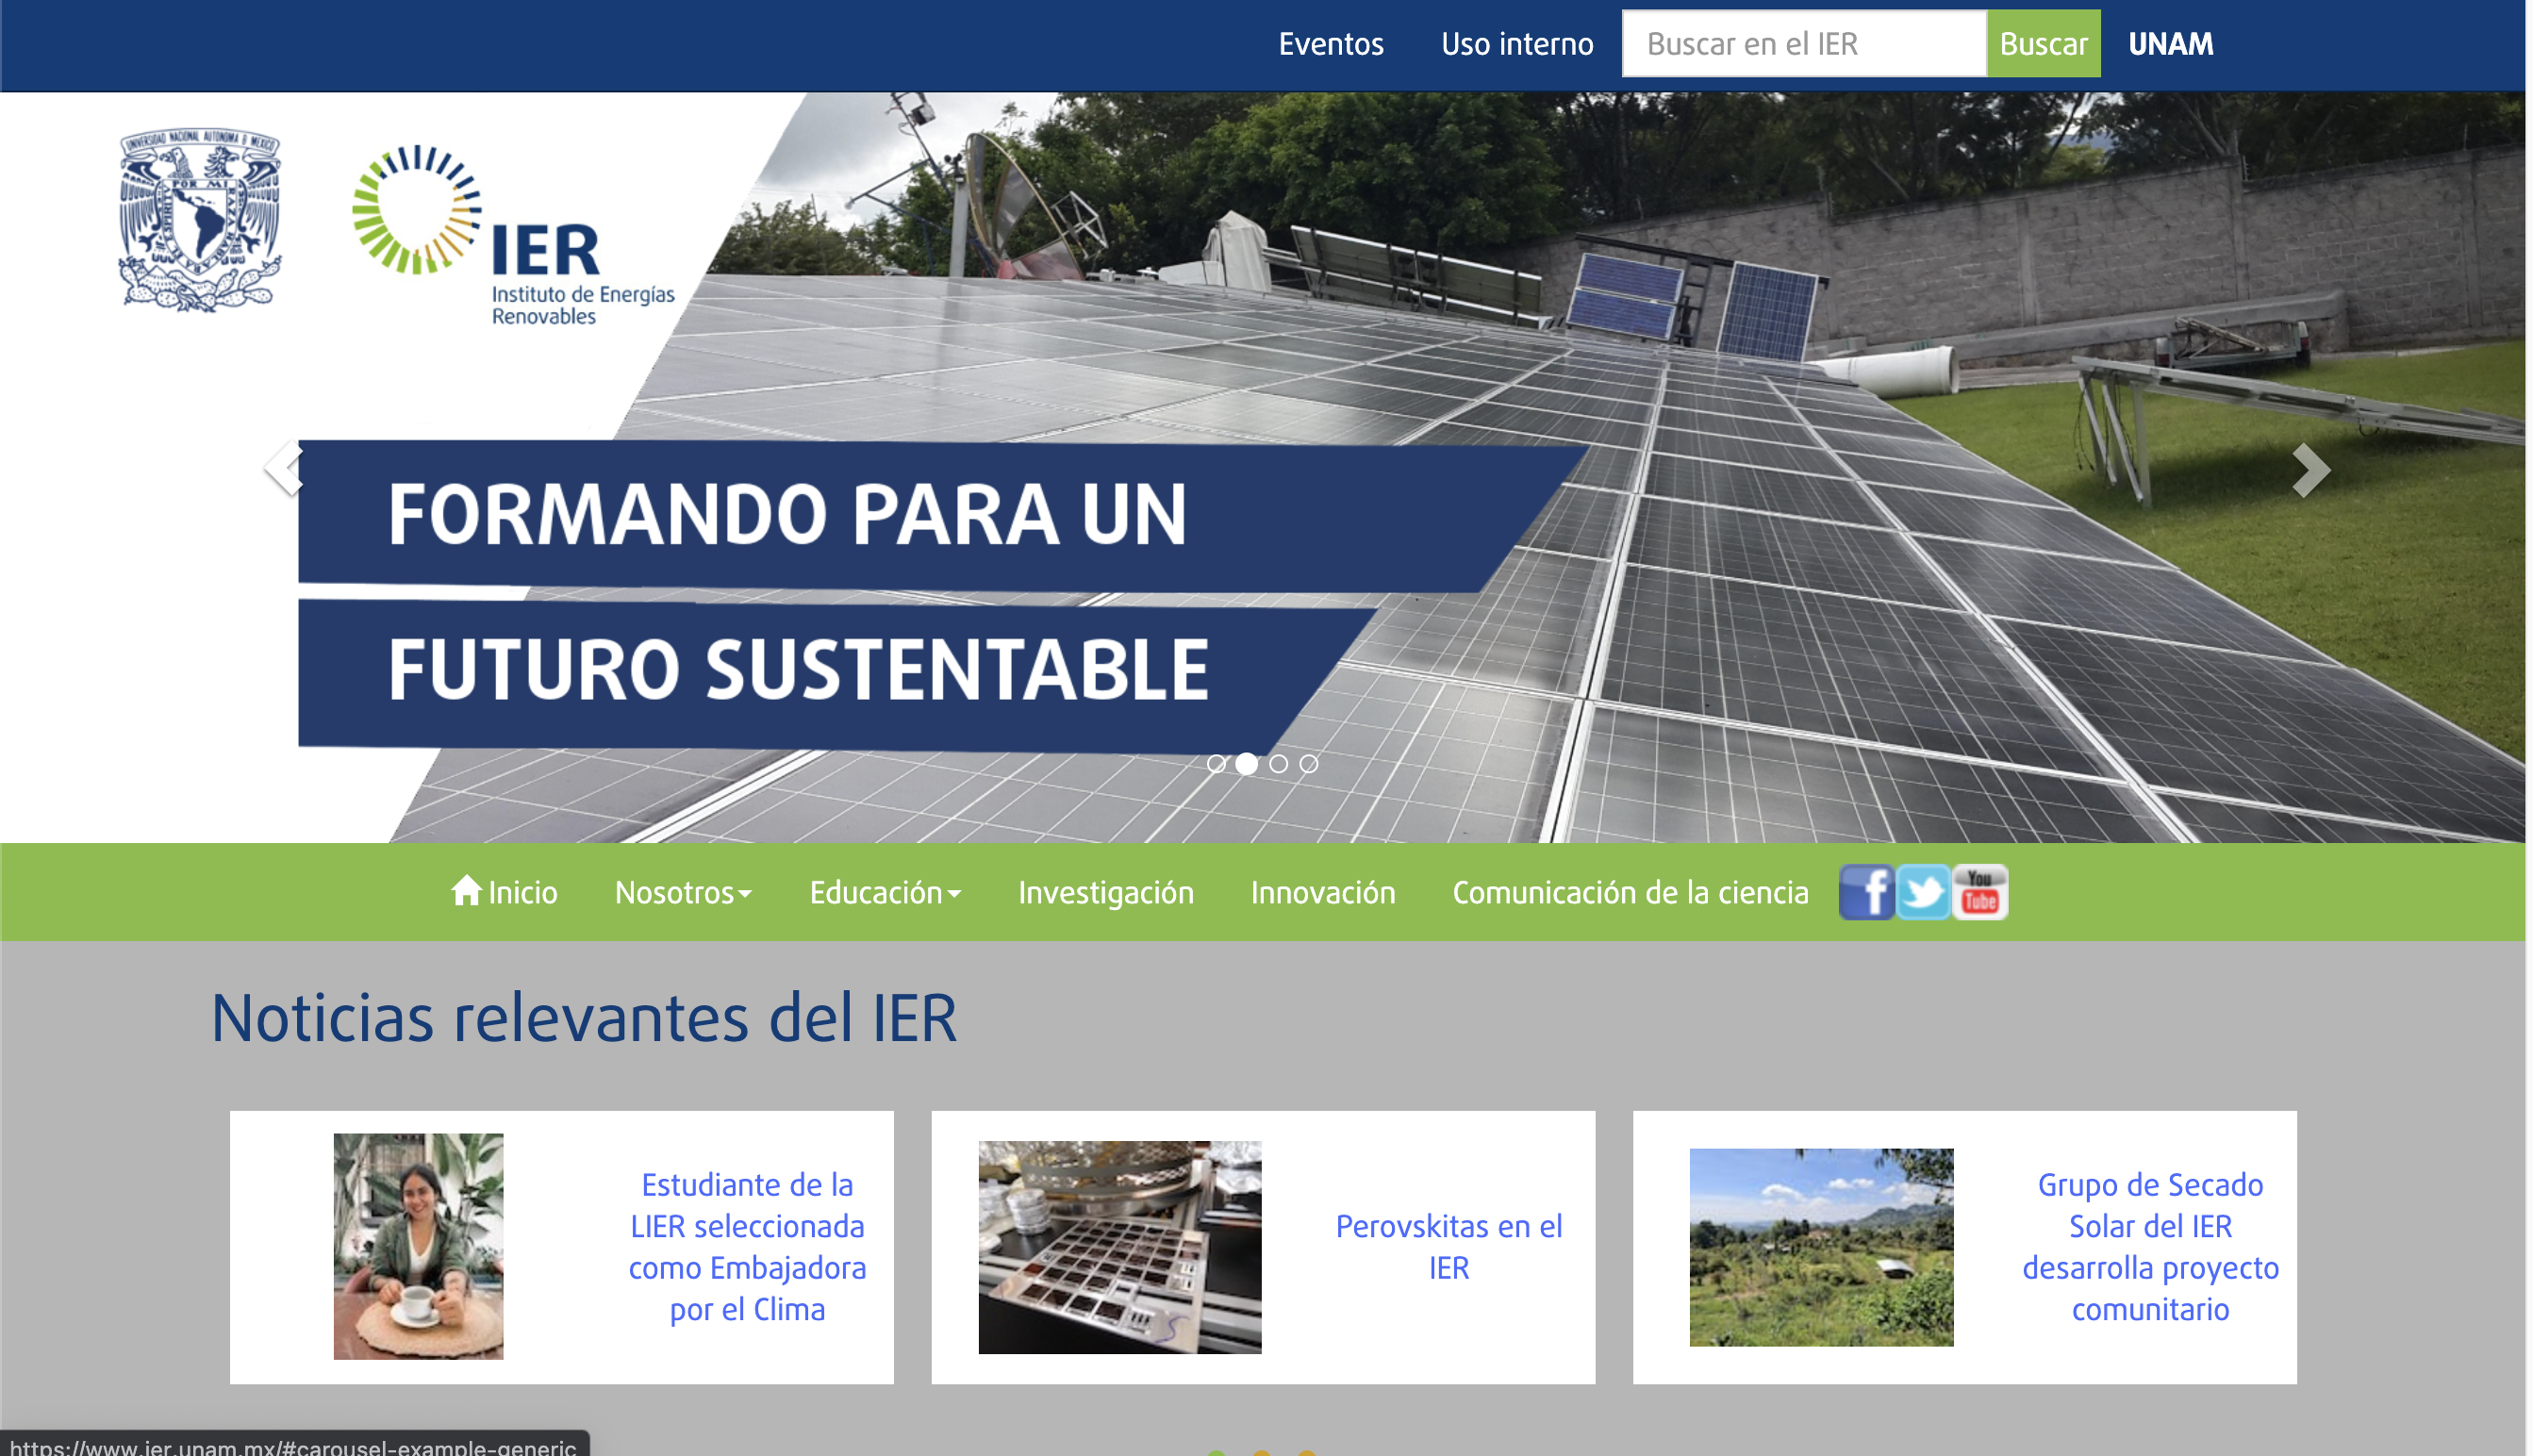
\includegraphics[scale=0.2]{ier_homepage}
 \caption{	
 Captura tomada de la página web del IER-UNAM.
 \label{fig:IER}
 }
 \end{figure}
 
 La figura se incluyó con el siguiente código
 \begin{verbatim}
 \begin{figure}
 \centering
 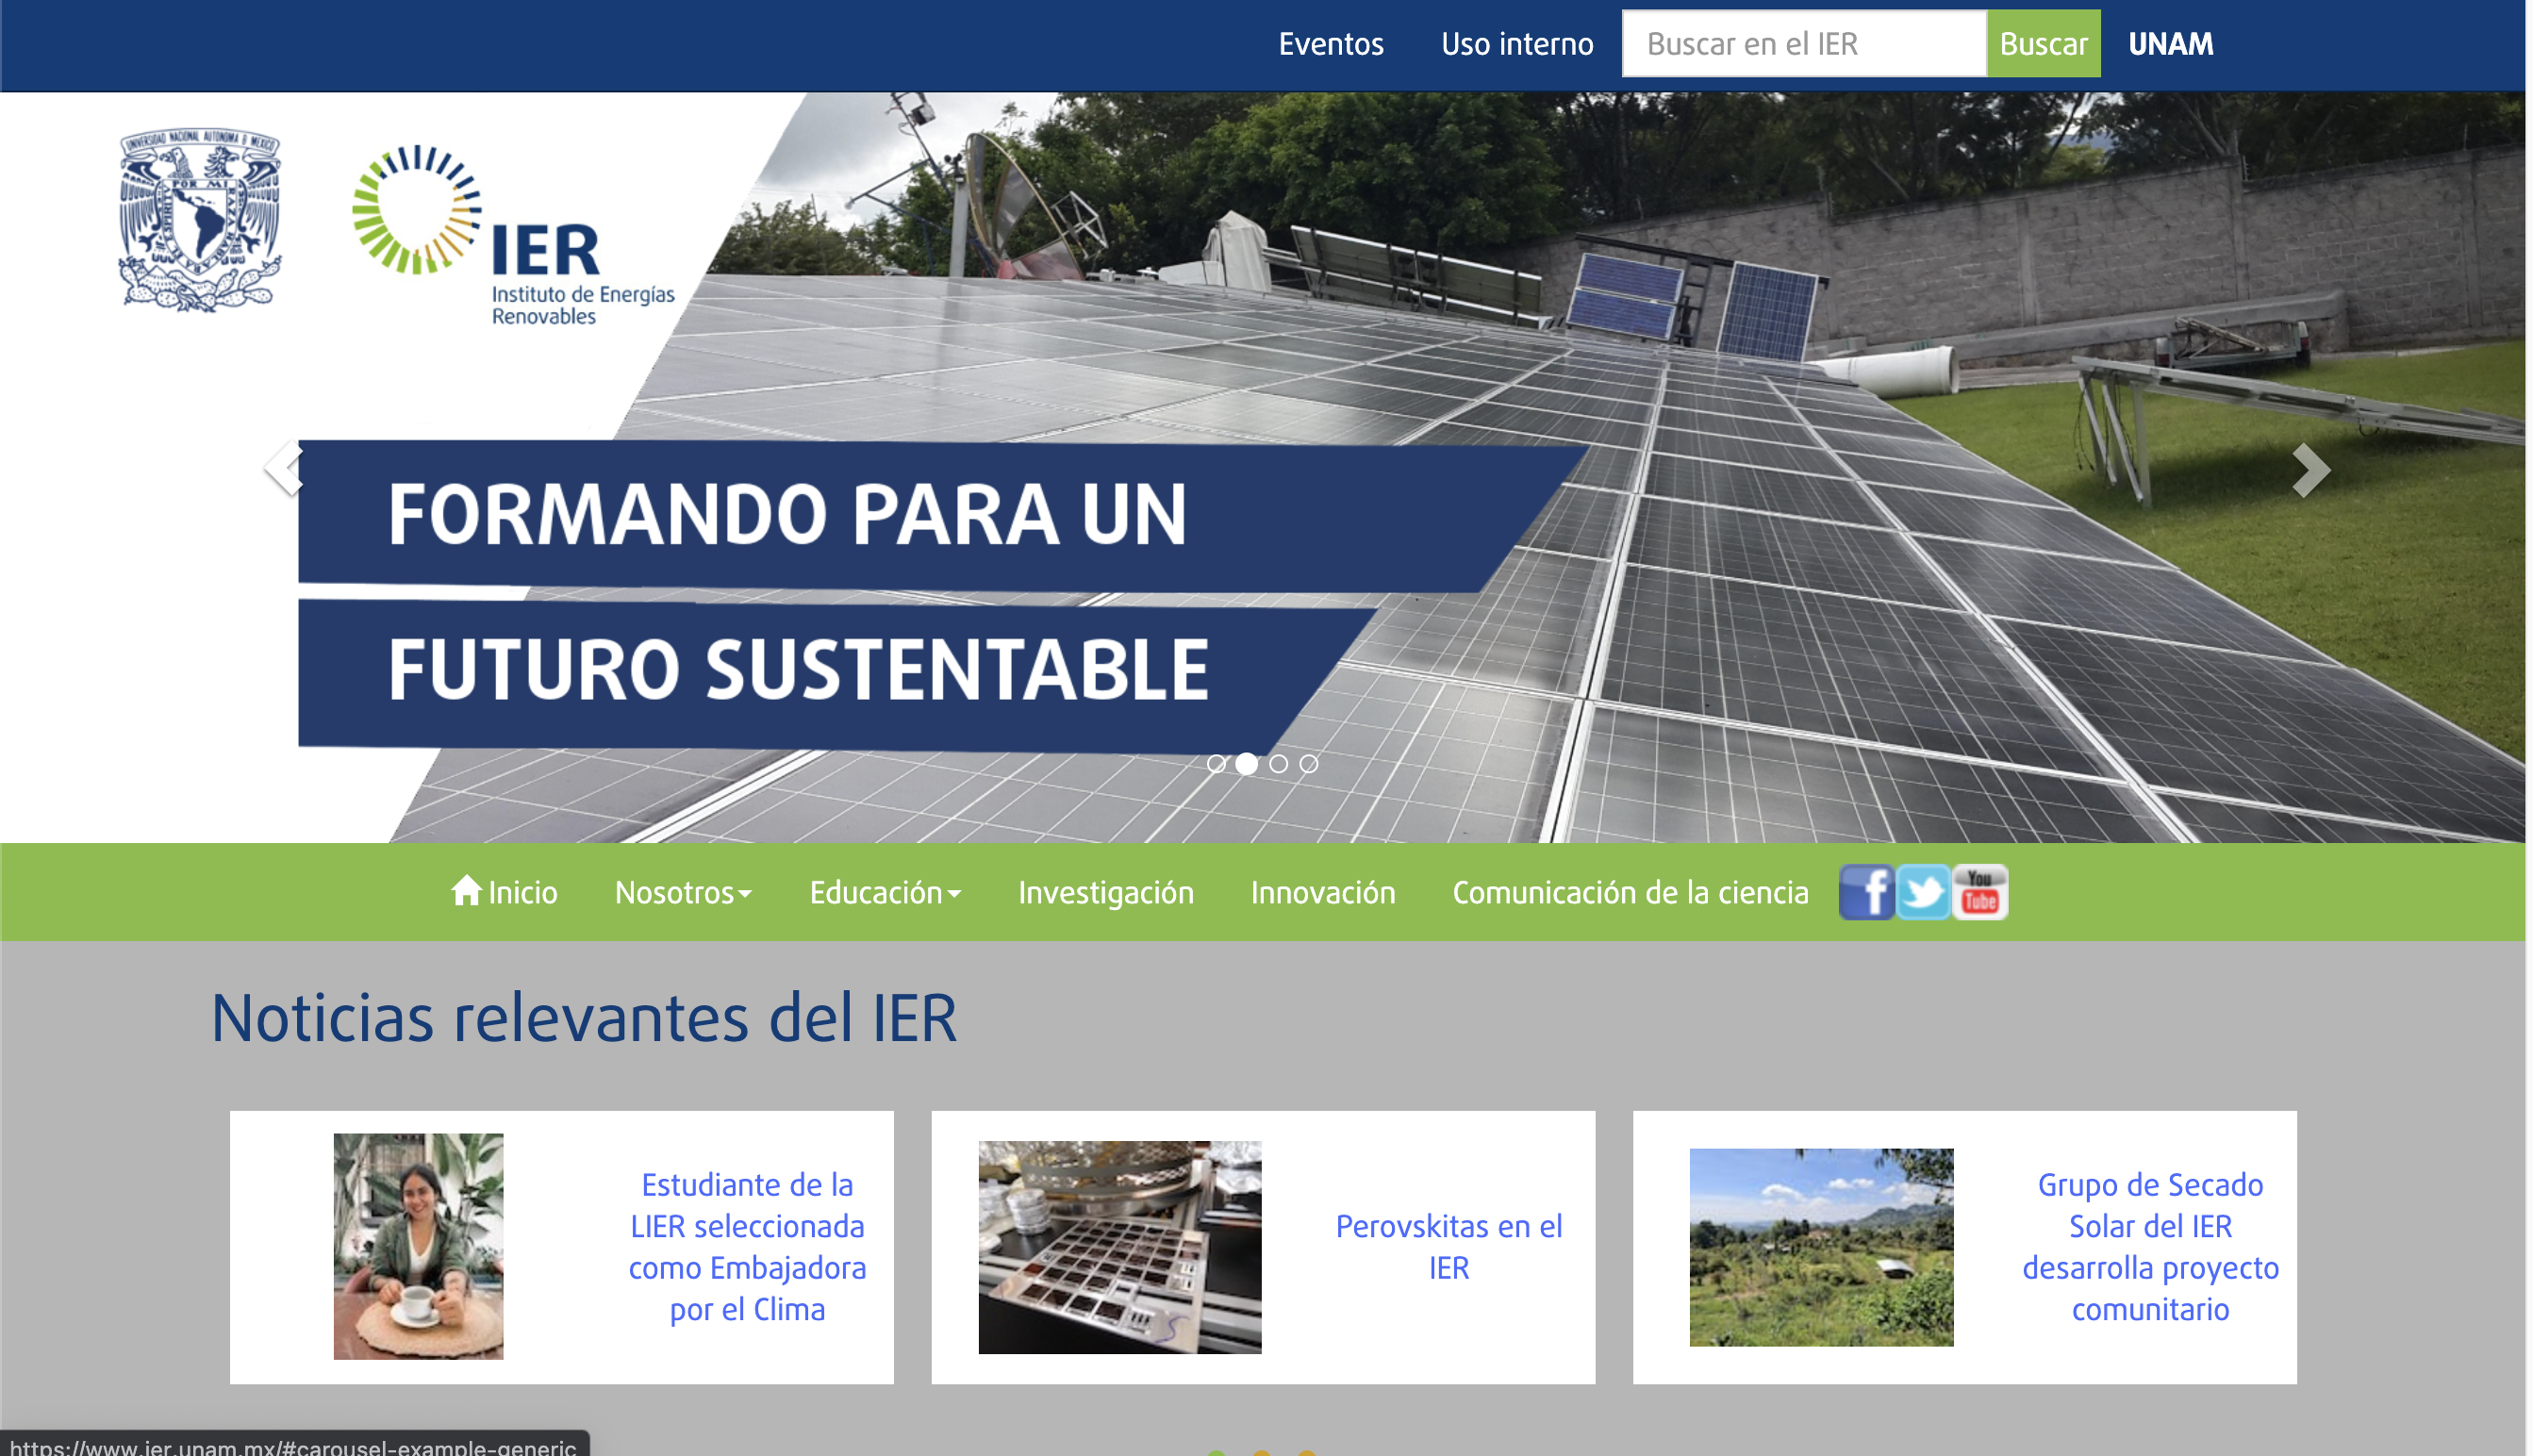
\includegraphics[scale=0.2]{ier_homepage}
 \caption{	
 Captura tomada de la página web del IER-UNAM.
 \label{fig:IER}}
 \end{figure}
 \end{verbatim}
 
Una práctica muy común que veo es que usan 
 \begin{verbatim}
 \begin{figure}[!ht]
 \end{verbatim}
 que le está diciendo a latex forzar a poner la figura en la misma página que el texto y en la parte superior de la página. Te recomiendo no usar esto y darle oportunidad a latex de acomodar las figuras de acuerdo a su criterio, además conforme tengas más texto, las figuras irán cambiando su lugar y se verá mejor.
\subsection{Figuras en pdf}
\subsection{Figuras en png/jpg}
\subsection{Figuras en epslatex}
\subsection{Figuras con gnuplot}
\subsection{Figuras en tex}
\subsection{Recomendaciones generales}
%\chapter{Levitaci'on ac'ustica}

\section{Introducci'on}

La posibilidad de mantener a una part'icula suspendendida por una onda ac'ustica en un
campo gravitacional, se conoce como levitaci'on ac'ustica. Uno de los aspectos m'as importantes,
es la posibilidad de recrear un ambiente de microgravedad para cualquier material existente en
la tierra. Un vez levitado, se pueden estudiar las propiedades del material. Por
ejemplo Trinh y Hsu~\cite{trinh86} usaron la levitaci'on ac'ustica para el c'alculo de la
densidad de diversos materiales. King~\cite{king34} estudi'o la fuerza ac'ustica ejercida sobre
una esfera en una onda estacionaria plana. M'as tarde, Gor'kov~\cite{gorkov62} desarroll'o una
expresi'on para calcular la fuerza ac'ustica de una esfera que se encuentra en una onda estacionaria
arbitraria. Para part'iculas cil'indricas, la teor'ia no ha avanzado de la misma manera, pues todos
los trabajos desarrollados consideran una onda estacionaria plana.
En el presente cap'itulo reportamos los resultados  de la simulaci'on
num'erica de la levitaci'on ac'ustica usando el m'etodo de la ecuaci'on de Boltzmann en redes (EBR).



En la secci'on~\ref{sec:antecedentes} presentamos los antecedentes sobre el estudio de fuerzas
ac'usticas actuando sobre una esfera y un cilindro. Los n'umeros adimensionales y los dispositivos
sobre los que realizamos las simulaciones num'ericas los presentamos en la secci'on~\ref{sec:adimensionales}.
Las simulaciones num'ericas de la levitaci'on ac'ustica para dos cavidades, una con reflector plano
y la otra con un reflector redondeado, ambas en dos dimensiones, las presentamos en
la secci'on~\ref{sec:simulaciones}.  
En la cavidad redondeada, cuando la cantidad de movimiento agregada por la fuente ac'ustica
es suficientemente grande, observamos que la din'amica de la part'icula presenta
un movimiento aperi'odico que puede ser ca'otico.
Rudnick y Barmatz~\cite{rudnick90} sugirieron que la part'icula levitada pod'ia tener
un comportamiento ca'otico sin aportar justificaci'on alguna.
Finalmente, en la secci'on~\ref{sec:conclusiones}, 
terminamos el cap'itulo con las conclusiones de las simulaciones num'ericas de la levitaci'on ac'ustica.
En este cap'itulo presentamos las primeras simulaciones num'ericas de la din'amica de una part'icula
levitada ac'usticamente. Como hemos mencionado anteriormente, la din'amica de la part'icula es el
resultado de su interacci'on con un fluido compresible, el cual simulamos usando el m'etodo de la
ecuaci'on de Boltzmann en redes.

\section{Antecedentes y teor'ia}
\label{sec:antecedentes}


En 1934, Louis V. King~\cite{king34} public'o el primer trabajo relacionado con la levitaci'on ac'ustica de
esferas. King realiz'o el c'alculo de la fuerza ac'ustica sobre una esfera r'igida fija sumergida en una
onda estacionaria plana y en una onda plana viajera. Para ambos casos, consider'o un fluido ideal y que el
radio de la esfera es muy peque~no comparado con la longitud de la onda plana. Tambi'en realiz'o el c'alculo
de la fuerza para el caso de una  esfera  libre de moverse bajo la acci'on del campo ac'ustico. 
King concluy'o que hay una relaci'on de densidades 'optima para la levitaci'on ac'ustica en una onda plana
estacionaria y tambi'en demostr'o que con los dispositivos de esa 'epoca la levitaci'on ac'ustica en aire de una 
esfera de corcho era imposible debido a las limitaciones t'ecnicas de los piezoel'ectricos. Sin embargo,
el c'alculo que realiz'o, considerando agua como medio de suspensi'on demostr'o que la levitaci'on ac'ustica,
al menos en teor'ia, ya era posible. Para este c'alculo, consider'o que la densidad de la part'icula $\rho_p$ 
entre la densidad del fluido $\rho_f$ era cercana a uno.


M'as tarde Yosiaka y Kawasima~\cite{yosiaka55} compararon resultados experimentales
de la fuerza ac'ustica sobre burbujas con la teor'ia desarrollada por King  y encontraron que la fuerza ac'ustica
puede ser de $10^5$ a $10^8$ veces m'as grande que la fuerza estimada por la f'ormula deducida por 
King. Esta diferencia, como demostraron Yosiaka {\it et al}, se debe a la compresibilidad
de la burbuja, as'i que desarrollaron una teor'ia para medir la fuerza ac'ustica sobre una esfera compresible en 
una onda ac'ustica viajera y una estacionaria, suponiendo en ambos caso un fluido  ideal y ondas ac'usticas planas. 
En los experimentos realizados, midieron la fuerza ac'ustica  sobre una burbuja 
de aire sumergida en agua a 1 atm'osfera y cero grados cent'igrados. En los experimentos realizados,
Las burbujas   se dirigieron a los nodos de presi'on de la onda plana estacionaria. 

En 1962  Gor'kov~\cite{gorkov62} present'o un m'etodo simple para 
determinar la magnitud de la fuerza ac'ustica sobre una part'icula esf'erica compresible en un campo
ac'ustico  estacionario arbitrario
para un fluido inviscido. Este m'etodo se puede aplicar para cualquier tipo de ondas, mientras
que los desarrollos anteriores se limitaban a ondas planas. Gor'kov encontr'o que la fuerza ac'ustica es derivable
de un potencial ac'ustico $U$ dado por
\BE\label{eq:gorkov}
U = 2\pi r^3 \rho_f \left( \frac{{\hat p^2}}{3\rho_f^2c_s^2} f_1 - \frac{{\hat v^2}}{2}f_2\right),
\EE
donde $r$ es el radio de la esfera, $\rho_f$ la densidad del fluido, $c_s$ la velocidad del sonido en el mismo, 
${\hat p^2}$ y ${\hat v}^2$ son las fluctuaciones cuadr'aticas medias de la presi'on y la velocidad en la onda, 
respectivamente. Adem'as $f_1 = 1 - (c_s^2\rho_f)/(c_p^2\rho_p)$ y 
$f_2=2(\rho_p-\rho_f)/(2\rho_p + \rho_f)$ donde $\rho_p$ y $c_p$ son la densidad y la velocidad del sonido 
en la part'icula. Para que la formula derivada por Gor'kov sea v'alida es condici'on necesaria que el radio
de la part'icula sea mucho menor que la longitud de onda, de  manera que la presencia de la part'icula no afecta el 
campo ac'ustico.

La levitaci'on ac'ustica de esferas s'olidas y compresibles (gotas) avanz'o r'apidamente, sobre todo en 
los llamados levitadores ac'usticos de un eje, que consisten en un piezo el'ectrico que emite la se~nal
ac'ustica y una superficie reflectora  que ayuda a formar la onda estacionaria donde se
coloca una part'icula. 
Oran {\it et al}~\cite{oran80} realizaron un estudio param'etrico de la cavidad, donde el objetivo
era aumentar la capacidad de levitaci'on, ya que hasta ese entonces la muestra m'as densa levitada era de
apenas $\rho \sim 5$ $gr/cm^3$. Oran {\it et al} encontraron emp'iricamente que con un reflector o un
piezoel'ectrico esf'erico se  duplicaba la fuerza ac'ustica bajo las mismas condiciones de operaci'on. Una combinaci'on
de ambos permiti'o levitar muestras de hasta 20 $gr/cm^3$ del mismo tama~no que las anteriores de 5 $gr/cm^3$. 



Leung {\it et al}~\cite{leung82} fueron los primeros en estudiar el
desplazamiento de la resonancia debido a la presencia de la part'icula dentro de una cavidad cuadrada
en tres dimensiones. Los estudios se realizaron en el r'egimen lineal, donde un an'alisis de Fourier
mostraba que los arm'onicos eran peque~nos. Encontraron que la frecuencia de resonancia es funci'on del 
tama~no de la esfera y de su posici'on, resultado de la exclusi'on del volumen por la presencia de 
la esfera y de las ondas reflejadas en la misma.  Otro aspecto importante es que en algunas ocasiones
la presencia de la part'icula suprimi'o la aparici'on de los arm'onicos.

Una de las primeras aplicaciones de la levitaci'on ac'ustica fue introducida por
Trinh y Hsu~\cite{trinh86}, quienes presentaron dos m'etodos para medir la densidad de un material usando 
la levitaci'on ac'ustica. Ambos  m'etodos tienen cuatro caracter'isticas importantes que son: (a) no existe
contacto entre la muestra a medir con cualquier objeto; (b) los resultados obtenidos son independientes
del tama~no y forma de la muestra; (c) se utiliza un esquema de comparaci'on por lo que no es necesario
conocer con precisi'on los par'ametros del campo ac'ustico; y (d) es necesaria una cantidad muy peque~na,
del orden de un microlitro o menos. El primer m'etodo supone que la magnitud de la presi'on ac'ustica y
su derivada respecto a la posici'on vertical son proporcionales al voltaje de entrada que alimenta al
piezoel'ectrico. Primero se levita una gota de l'iquido con densidad $\rho_{p1}$, compresibilidad $\beta_{p1}$
y se levita en una posici'on $y_1$ con un voltaje $V_1$. Despu'es una gota con propiedades desconocidas
$\rho_{p2}$, $\beta_{p2}$ se hace levitar en la misma posici'on $y_1$ que la muestra anterior con un voltaje  
$V_2$. La relaci'on de voltajes est'a relacionada por
\BE
\left( \frac{V_1}{V_2}\right)^2 =  
\frac{G(\beta_{p1}/\beta_{f1},\rho_{p1}/\rho_{f1})}{G(\beta_{p2}/\beta_{f2},\rho_{p2}/\rho_{f2})},
\EE
donde $\rho_{f1}$ y $\beta_{f1}$ se refieren a las propiedades del fluido donde la muestra
es levitada y que puede ser diferente para ambos experimentos, por eso
aparecen $\rho_{f2}$ y $\beta_{f2}$. La relaci'on de compresibilidad--densidad $G$ se define como
\BE
G =
\frac{ | 1-\rho_p/\rho_f |}
{\beta_p/\beta_f-(5\rho_p - 2\rho_f)/(2\rho_p + \rho_f)}.
\EE 
De esta manera, si conocemos solamente una de las propiedades de la muestra levitada $\rho_{p1}$ o 
$\beta_{p1}$ podemos determinar la otra, seg'un sea el caso. El segundo m'etodo se basa en la din'amica
de la part'icula. En un ambiente de gravedad cero, una part'icula en un campo ac'ustico siempre se localiza
en el nodo de presi'on, independientemente de la intensidad del campo ac'ustico. Bajo estas condiciones, el primer
m'etodo basado en la relaci'on existente entre el voltaje de entrada del piezoel'ectrico ya no es 'util. El
concepto b'asico de este m'etodo se basa en la determinaci'on de la frecuencia  caracter'istica
de una masa acoplada a una fuerza restitutiva, usualmente proporcionada por un resorte. En la parte
lineal, la frecuencia  del sistema masa--resorte est'a dada por
\BE
\omega = (K/m)^{1/2},
\EE 
donde $K$ es la constante del resorte y $m$ es la masa del objeto. 
Entonces la fuerza ac'ustica para peque~nos desplazamientos de la posici'on $z$ donde la fuerza ac'ustica es cero, 
\BE
F = -K z,
\EE
donde
\BE
K =\frac{20\pi^2 p_o^2}{6\lambda\rho_p c_s^2}k r^3z.
\EE
En la expresi'on anterior $r$ es el radio de la esfera, $c_s$ la velocidad del sonido, $\rho_p$ la densidad de la part'icula
levitada, $k=2\pi/\lambda$ es el n'umero de onda y $p_o$ la amplitud m'axima  de la presi'on en la onda ac'ustica. 
Entonces, para valores peque~nos de $z$ la fuerza ac'ustica
se puede considerar lineal, y la posici'on de equilibrio coincide con el nodo de presi'on cuando los efectos
gravitacionales son despreciables. Se puede deducir que la frecuencia  $\omega_2$ de una muestra con 
densidad  $\rho_{p2}$ y volumen $V_2$ est'a relacionada de la siguiente manera con una muestra de densidad
conocida $\rho_{p1}$ de la siguiente manera
\BE
\frac{\rho_{p1}}{\rho_{p2}} = \left( \frac{\omega_2}{\omega_1} \right)^2 \left( \frac{V_1}{V_2} \right)^2
\frac{\cos (4\pi z_1/\lambda)}{\cos (4\pi z_2/\lambda)},
\EE
donde $z_1$ y $z_2$ son las posiciones de equilibrio de las part'iculas levitadas. Para el caso de un ambiente
en gravedad cero, $z_1=z_2$ para cualquier valor de $V$, adem'as, si las part'iculas son del mismo
volumen $V_1 = V_2$, entonces las densidades est'an relacionadas por el cuadrado de las frecuencias, las cuales 
se miden experimentalmente.  
Trinh y Hsu reportaron que el m'etodo basado en la relaci'on de voltaje tiene una precisi'on de 1\%, pero que no es muy bueno
tomando en cuenta los est'andares de medici'on de densidad~\cite{trinh86}.  Para el segundo m'etodo, basado en la
frecuencia de resonancia de la part'icula, reportaron errores de hasta un 6\%.  Si bien este error no es tan bueno
como se esperaba, la gran ventaja es que esta t'ecnica se puede implementar en ambientes de gravedad reducida
o nula.

Rudnick y Barmatz~\cite{rudnick90}, al igual que Leung {\it et al}~\cite{leung82}, 
realizaron un estudio sobre el desplazamiento de la resonancia debido a la presencia de la part'icula esf'erica
en el campo ac'ustico con una onda plana.   De acuerdo a Rudnick y Barmatz, el desplazamiento de la 
resonancia ocasiona inestabilidades 
en el movimiento de la part'icula. Estas inestabilidades pueden
dar paso a dos comportamientos, el primero ocasiona que la oscilaci'on de la part'icula crezca hasta alcanzar una
amplitud finita y estabilizarse. En el segundo comportamiento, la oscilaci'on de la part'icula crece hasta desestabilizarse
completamente y caer. Rudnick y Barmatz modelaron el comportamiento de la part'icula con la siguiente ecuaci'on
\BE
m \frac{d^2 z(t)}{dt^2} + \left( \sigma - \Gamma [z(t)] \right) \frac{dz(t)}{dt} 
+ f_o(z(t)) - mg =0,
\EE
donde $z(t)$ es la posici'on de la part'icula a partir de la posici'on de equilibrio, $\sigma {\dot z}(t)$ 
es una fuerza debida a la viscosidad del fluido , $f_o(z(t))$ es la fuerza ac'ustica que act'ua sobre la part'icula  
y  $\Gamma [z(t)] {\dot z}(t) $ es una fuerza que no se explica su origen en el trabajo de Rudnick y Barmatz. Si
$\Gamma [z(t)] {\dot z}(t) < \sigma {\dot z}(t)$  hay disipaci'on, pero en el caso contrario,
hay una amplificaci'on de la oscilaci'on que desestabiliza la levitaci'on.
Tambi'en sugirieron que la din'amica de la part'icula
puede ser ca'otica pero no aportaron pruebas o justificaci'on alguna.

Xie y Wei~\cite{xie01}, al igual que Oran {\it et al}~\cite{oran80}, realizaron un estudio param'etrico de un levitador
ac'ustico de un eje  con la finalidad de incrementar la fuerza ac'ustica. La diferencia principal entre estos
dos trabajos es que Xie y Wei se apoyaron en una soluci'on num'erica del problema y lo verificaron 
experimentalmente. En condiciones normales de gravedad, Oran {\it et al} levitaron una part'icula de
platino ($\rho=20 g/cm^3$) pero no reportaron las dimensiones. Xie y Wei reportaron haber 
levitado una part'icula de tungsteno ($\rho=18.92 g/cm^3$) con un radio de $r=1.5$mm con un piezoel'ectrico
plano y un reflector con superficie curva.  En trabajos posteriores, Xie {\it et al}~\cite{xie02,xie02c} reportaron
haber levitado iridio ($\rho=22.6 gr/cm^3$) y mercurio ($\rho=13.6 gr/cm^3$) que son el s'olido  y el l'iquido m'as
densos   que hay en la tierra. En un art'iculo publicado recientemente, 
Xie {\it et al}~\cite{xie06}  presentaron la levitaci'on de peque~nos organismos vivientes como una
hormiga, un escarabajo y hasta un pez peque~no que van de los 5 a los 10 $mm$. 
 

Los primeros trabajos sobre cilindros en un campo ac'ustico, fueron los de
Awatani~\cite{awatani55} y Hasegawa {\it et al}~\cite{hasegawa88}, quienes  reportaron  resultados
num'ericos de la fuerza ac'ustica en una onda viajera para un cilindro r'igido y uno el'astico, respectivamente. Pero
hasta ese entonces, no se hab'ian reportado resultados para el caso de un cilindro en una onda ac'ustica estacionaria.
Wu {\it et al}~\cite{wu90} fueron los primeros que reportaron una expresi'on anal'itica para un cilindro r'igido dentro de una
onda estacionaria. El desarrollo se bas'o en el trabajo de King~\cite{king34} usando coordenadas cil'indricas. 
Wu {\it et al} reportaron que la fuerza ejercida en un campo ac'ustico por unidad de longitud  para un cilindro es
\BE\label{eq:force-wu}
F = \left( \frac{1-\beta} {2(1+\beta)} + 1 \right) v \omega \left( \frac{p_o^2} {\rho_f c_s^2} \right)^2 \sin (2kh)
\EE
donde $\beta=\rho_f/\rho_p$ es la relaci'on de densidades entre el fluido $\rho_f$ y la part'icula $\rho_p$, $p_0$ es la
presi'on est'atica, $\omega$ es la frecuencia de la onda estacionaria, $v$ es la amplitud de la velocidad, $c_s$ es la
velocidad del sonido en el fluido, $k$ el n'umero de onda y $h$ es la distancia a la cual se encuentra el centro del 
cilindro de la fuente ac'ustica. En la ecuaci'on anterior no se tom'o en cuenta el
radio $r$ del cilindro porque se considera que es muy peque~no comparado con la longitud de onda ($kr \ll 1$).

Wei {\it et al}~\cite{wei04} calcularon la fuerza ac'ustica actuando sobre un cilindro infinito de radio $r$ sobre
una onda estacionaria plana.
El centro del cilindro se encuentra en $z=0$ y el antinodo de presi'on m'as cercano 
se encuentra en $z=-h$, por lo que la fuerza ac'ustica por unidad de longitud en el cilindro es
\BE\label{eq:force-wei} 
F = \frac{r}{4}p^2_f \beta_f \sin (2k h ) Y_{st},
\EE
donde $p_f$ es la amplitud m'axima de la presi'on , $\beta_f=1/(\rho_f c_s^2)$ es la compresibilidad del fluido y $k$
el n'umero de onda. 
El t'ermino $Y_{st}$ lo desarrollaron para el caso de un cilindro con compresibilidad 
$\beta_p=1/(\rho_p c_p^2)$, donde $\rho_p$ son la densidad  y  $c_p$ la velocidad del s'onido en la part'icula. 
La aproximaci'on para el t'ermino $Y_{st}$ es
\BE
Y_{st} = \pi k r (f_1 + f_2),
\EE
donde 
\BE
f_1=1-(\beta_p/\beta_f)
\EE 
y
\BE
f_2 = 2 \left( \frac{\rho_p/\rho_f -1}{\rho_p/\rho_f +1} \right).
\EE
Para el caso de un cilindro incompresible, simplemente $f_1 = 1$. 

Casi a la par del art'iculo publicado por Wei {\it et al}, Haydock~\cite{haydock05,haydock05b} public'o dos
art'iculos sobre el c'alculo  de la fuerza ac'ustica  sobre un cilindro inmovil en una onda estacionaria plana. 
En el primer trabajo, encontr'o que la fuerza ac'ustica por unidad de longitud $F$ est'a dada por
\BE
F =  \PROM{F_\phi} + \PROM{F_k} + \PROM{F_c}.
\EE
donde la fuerza  es suma de las contribuciones promediadas sobre el tiempo de las fuerzas debidas a la energ'ia potencial ac'ustica 
$\PROM{F_\phi}$, a la energ'ia cin'etica $\PROM{F_k}$ y al movimiento del cilindro $\PROM{F_c}$. Estas contribuciones se
definen como
\BE
\PROM{F_\phi} = -\frac{r\rho_f}{2 c_s^2} \int_0^{2\pi} \PROM{\dot{\psi^2}} \cos \theta d\theta,
\EE
\BE
\PROM{F_k} = -\frac{r\rho_f}{2} \int_0^{2\pi} \PROM{u^2} \cos \theta d\theta,
\EE
y
\BE
\PROM{F_c} = -r \rho_f \int_0^{2\pi} \PROM{\vu \cdot \vv_p} \cos \theta d\theta,
\EE
donde las integrales son alrededor del cilindro y  
$\psi$ es el potencial de la velocidad, $\vu$ la velocidad del fluido alrededor del cilindro
y $\vv_p$ la velocidad del cilindro. 

En el segundo trabajo  report'o la medici'on de la fuerza ac'ustica debida a una onda estacionaria en simulaciones num'ericas
usando el m'etodo de la ecuaci'on de Boltzmann en redes (EBR). Haydock utiliz'o el m'etodo propuesto por Ladd~\cite{ladd94} para
implementar la simulaci'on de una part'icula s'olida dentro del m'etodo de la EBR. Sus resultados mostraron una diferencia
que va de un 4\% a un 146\%  entre la teor'ia y los resultados de las simulaciones num'ericas para la fuerza actuando sobre 
un cilindro.  La raz'on de la discrepancia entre teor'ia y
simulaciones radica en que la teor'ia es v'alida siempre y cuando el grosor de la capa l'imite ac'ustica sea mucho menor
al tama~no de la part'icula y cuando el error fue grande, este criterio no se cumpli'o. Haydock tambi'en realiz'o
simulaciones num'ericas de una part'icula cil'indrica libre dentro de una onda estacionaria plana en ausencia de un campo
gravitacional externo. Como era de esperarse, al colocar la part'icula dentro de una onda estacionaria 
'esta se dirigi'o al nodo de presi'on donde la sumatoria de fuerzas ac'usticas es cero.

El desarrollo en la teor'ia para cilindros en un campo ac'ustico no ha avanzado de la misma manera
que lo ha hecho la teor'ia para esferas. Uno de los logros m'as importantes en la teor'ia ac'ustica
ha sido la formulada por Gor'kov, que permite calcular el potencial ac'ustico para una onda cualquiera, logro
que no se ha igualado en la teor'ia para cilindros. La  teor'ia ha sido desarrollada partiendo de
flujos potenciales y ondas planas con cilindros inmoviles. Por otro lado, 
los experimentos num'ericos para cilindros se han realizado
en ondas planas estacionarias y en ausencia de fuerza de cuerpo externa, por lo que la part'icula liberada
se dirige a los nodos de presi'on o antinodos de velocidad. Adem'as, las simulaciones num'ericas con la EBR
realizadas por Haydock, se us'o el esquema para la simulaci'on de part'iculas s'olidas propuesto por 
Ladd~\cite{ladd94,ladd94b}, cuando se sabe que hay esquemas m'as adecuados~\cite{aidun98}.
 



\section{N'umeros adimensionales y dispositivo experimental}
\label{sec:adimensionales}

Los  resultados de las simulaciones num'ericas los reportamos en las cantidades adimensionales
que definimos a continuaci'on.
Para el problema de una part'icula circular
s'olida en un campo ac'ustico las distancias o posiciones adimensionales, indicadas con un
asterisco en el super'indice, son
\BE
\textbf x^\ast = \textbf x k,\qquad r^\ast = rk \qquad L^\ast = Lk,
\EE
donde el $\textbf x$ es la posici'on de la part'icula de radio $r$ y $L$ es una
distancia cualquiera. Las distancias se adimensionalizan con el n'umero de onda $k= 2\pi/\lambda$,
donde $\lambda$ es la longitud de la onda ac'ustica. El tiempo adimensional es
\BE
t^\ast = \frac{t}{T},
\EE  
donde $T=2\pi/\omega$ es el peri'odo, $\omega=2\pi c_s/\lambda$ la frecuencia angular de la
onda ac'ustica y $c_s$ la velocidad del sonido en el fluido. Como explicamos en la secci'on anterior,
el levitador de un eje consiste en una fuente que genera la onda ac'ustica y un reflector que
ayuda a formar la onda estacionaria.
En las simulaciones num'ericas, se agrega una cantidad de movimiento $P=P_o \cos \omega t$ en cada
nodo. La cantidad de movimiento adimensional agregada por la fuente ac'ustica es
\BE
P^\ast = \frac{PkT}{\pi r^2 \rho_f},
\EE
donde $\rho_f$ es la densidad del fluido. 
La velocidad adimensional es
\BE
\vu^\ast = \frac{\vu}{v_{max}},
\EE
donde $v_{max}$ es la velocidad m'axima del fluido dentro de la cavidad.




\begin{figure} 


\centering
%\begin{pspicture}(9,6)
%%\psgrid
%%
%\psline(1,1)(3,1)
%\psline(1,4)(3,4)
%\psline{<->}(1,3.75)(1,4.25)
%\psline{<->}(1.5,3.75)(1.5,4.25)
%\psline{<->}(2,3.75)(2,4.25)
%\psline{<->}(2.5,3.75)(2.5,4.25)
%\psline{<->}(3,3.75)(3,4.25)
%\rput[C](2,0){(a)}	
%%
%\psline[linewidth=0.1mm,linestyle=dashed]{|-|}(1,4.5)(3,4.5)
%\rput[C](2,4.7){$B^\ast$}
%\psline[linewidth=0.1mm,linestyle=dashed]{|-|}(.5,1)(.5,4)
%\rput[C](.3,2.5){$H^\ast$}
%%
%\psline(6,4)(6.5,4)(6.5,3.5)(7.5,3.5)(7.5,4)(8,4)
%\psline (6,2)(6,1)(8,1)(8,2)
%\psarc(7,3.5){1.8}{236}{304}
%\psline{<->}(6.75,3.25)(6.75,3.75)
%\psline{<->}(7.,3.25)(7.,3.75)
%\psline{<->}(7.25,3.25)(7.25,3.75)
%\rput[C](7,0){(b)}
%%
%\psline[linewidth=0.1mm,linestyle=dashed]{|-|}(6.5,4.5)(7.5,4.5)
%\rput[C](7,4.7){$B^\ast$}
%\psline[linewidth=0.1mm,linestyle=dashed]{|-|}(5.5,3.5)(5.5,1.7)
%\rput[C](5.3,2.5){$H^\ast$}
%\psline[linewidth=0.1mm,linestyle=dashed]{|-|}(6,.8)(8,.8)
%\rput[C](7,.5){$W^\ast$}
%\psline[linewidth=0.1mm,linestyle=dashed]{|->}(7,4)(8,2)
%\rput[C](8.1,2.4){$R^\ast$}
%\psline[linewidth=0.1mm,linestyle=dashed]{|-|}(8.3,4)(8.3,3.5)
%\rput[C](8.6,3.5){$h_b^\ast$}
%\psline[linewidth=0.1mm,linestyle=dashed]{|-|}(8.3,1)(8.3,2)
%\rput[C](8.6,1.25){$h_a^\ast$}
%\psline[linewidth=0.1mm]{->}(4.5,3)(4.5,2)
%%\rput[C](4.5,1.75){$g$}
%%
%\end{pspicture}

\caption{\label{fig:cavidades}
(a) Levitador ac'ustico de un eje con un reflector plano. La fuente del levitador se encuentra
localizada en la parte superior de la cavidad; $B^\ast= 5.092$  y $H^\ast$ puede variar. 
(b) Levitador ac'ustico de un eje con un reflector redondeado con 
$W^\ast=10.184$, $B^\ast=5.092$, $R^\ast=12.244$, $h_b^\ast =0.1377$, 
y $h_a^\ast=0.01028$. Para ambas cavidades, se fijaron los siguientes par'ametros de EBR para 
todas las simulaciones num'ericas $\tau=0.6$, $\rho_f=0.6$ y en un espacio bidimensional usando la malla $D2Q9$.}
\end{figure}
Las simulaciones num'ericas de levitaci'on ac'ustica de un cilindro, al que 
llamamos  part'icula   en lo que sigue, las llevamos  a cabo en dos
cavidades bidimensionales diferentes, que mostramos en las figuras~\ref{fig:cavidades} (a) y (b). 
La cavidad de la figura~\ref{fig:cavidades} (a)
corresponde a un levitador ac'ustico de un eje  con una fuente ac'ustica plana y con un reflector tambi'en  
plano en la parte inferior.
La cavidad redondeada de la figura~\ref{fig:cavidades} (b) tiene la forma y dimensiones reportadas
por Xie y Wei~\cite{xie01}, quienes realizaron experimentos en una cavidad tridimensional, 
mientras que las simulaciones num'ericas son bidimensionales.


\section{Levitaci'on ac'ustica}
\label{sec:simulaciones}

Como mencionamos en la secci'on anterior, las simulaciones num'ericas las realizamos en dos
cavidades. La cavidad plana se simul'o en una malla de  $163 \times 201$ nodos y 
la cavidad redondeada en una malla de $901 \times 253$ nodos. El tama~no de malla se
escogi'o en funci'on del radio de la part'icula, dado que es el elemento simulado  m'as peque~no
en el problema. El radio de la part'icula fue establecido en $r=9.5$ nodos y en forma adimensional
en $r^\ast=0.25$ al igual que los experimentos realizados 
por Xie {\it et al} y el resto de los tama~nos de la cavidad se escalaron en funci'on del radio. 
En el ap'endice A  mostramos los experimentos realizados para determinar el tama~no de la part'icula,
en la secci'on A.3. 
Los reflectores  y dem'as paredes para ambas cavidades los simulamos con la
condici'on a la frontera del rebote hacia atr'as, mientras que 
la fuente ac'ustica se genera agregando cantidad de movimiento en la direcci'on vertical, ambas
presentadas en la secci'on~\ref{sec:noslip}. Para la cavidad
plana, las simulaciones num'ericas las realizamos con condiciones peri'odicas a la frontera en la direcci'on
horizontal. En la cavidad redondeada, colocamos paredes con condici'on de no deslizamiento usando el rebote
hacia atr'as. Los par'ametros de densidad y viscosidad del fluido los mantuvimos constantes para 
todas las simulaciones y sus valores son $\rho_f=0.6$ y $\nu=0.0333$, respectivamente. 

Para el caso de una onda plana las frecuencias de resonancia son
\BE
\omega = \frac{2\pi c_s (2n-1)}{4H},
\EE
donde $H$ es la altura de la cavidad, $c_s$ es la velocidad del sonido en el fluido  
y $n=1,2,\ldots$ es el modo resonante. Para encontrar los modos resonantes 
en la cavidad redondeada, realizamos simulaciones num'ericas variando la altura de la cavidad 
y encontramos el valor m'aximo de la velocidad una vez que se ha formado una onda estacionaria, 
como vemos  de la figura~\ref{fig:resonancia}, donde mostramos los primeros dos  modos resonantes
localizados en $H^\ast/\pi =1.09$ y $2.14$ para la cavidad redondeada.
Como hab'iamos dicho anteriormente, los par'ametros geom'etricos de la cavidad redondeada son los correspondientes 
a los presentados por Xie y Wei~\cite{xie01}, quienes reportaron que los primeros modos resonantes para 
una cavidad tridimensional son  $H^\ast/\pi=1.20$  y $2.30$. 
Para ambas cavidades, el n'umero del modo resonante, corresponde al n'umero de nodos de presi'on dentro de la 
cavidad. En un nodo de presi'on, la amplitud de la oscilaci'on  en la presi'on es cero y la sumatoria de fuerzas ac'usticas
en esa posici'on tambi'en es cero. En esa mismo posici'on se localiza un antinodo de velocidad, donde la amplitud
de la oscilaci'on en la velocidad es m'axima.

\begin{figure} 
%GNUPLOT: LaTeX picture with Postscript
\begin{picture}(0,0)%
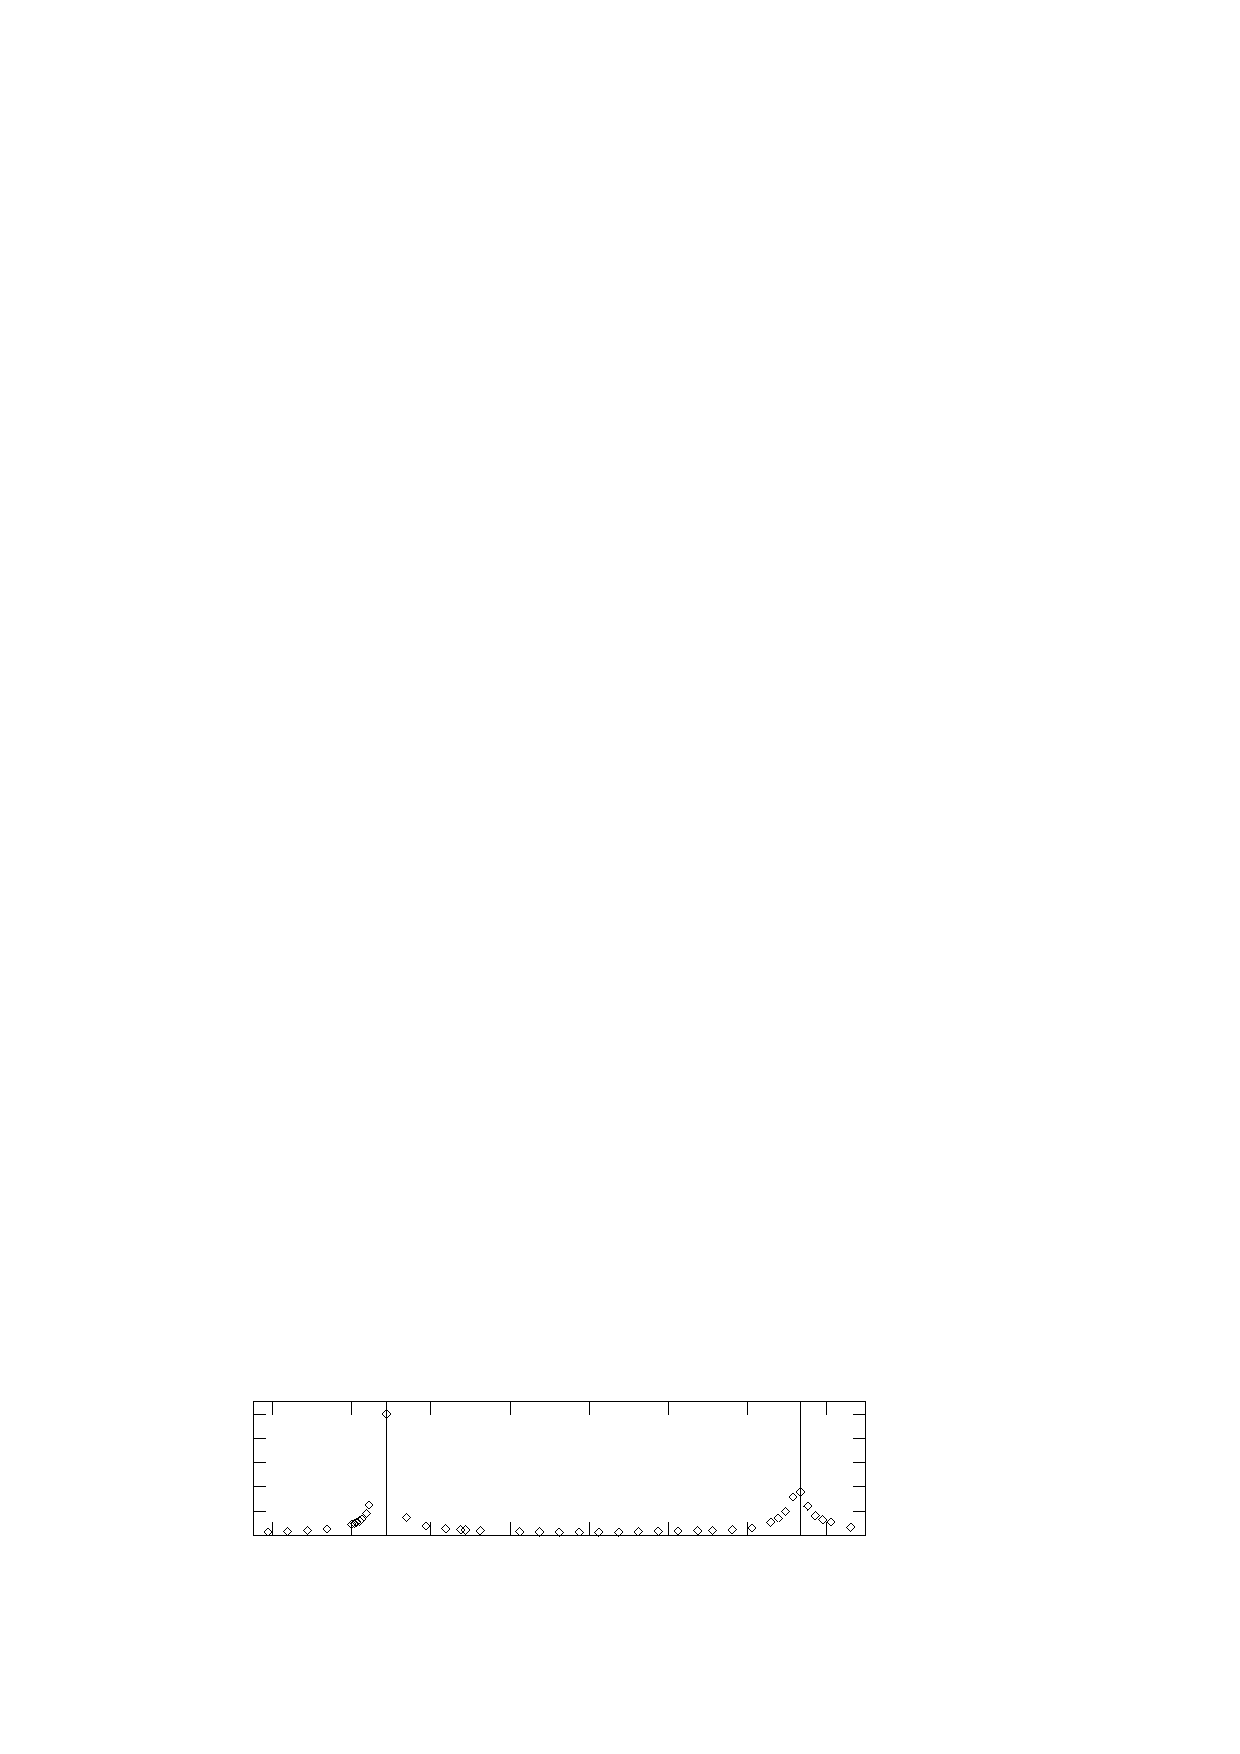
\includegraphics{eps/resonancia}%
\end{picture}%
\begingroup
\setlength{\unitlength}{0.0200bp}%
\begin{picture}(18000,5400)(0,0)%
\put(2200,1650){\makebox(0,0)[r]{\strut{} 0.0}}%
\put(2200,2232){\makebox(0,0)[r]{\strut{} 0.2}}%
\put(2200,2814){\makebox(0,0)[r]{\strut{} 0.4}}%
\put(2200,3395){\makebox(0,0)[r]{\strut{} 0.6}}%
\put(2200,3977){\makebox(0,0)[r]{\strut{} 0.8}}%
\put(2200,4559){\makebox(0,0)[r]{\strut{} 1.0}}%
\put(2949,1100){\makebox(0,0){\strut{} 0.8}}%
\put(4846,1100){\makebox(0,0){\strut{} 1.0}}%
\put(6743,1100){\makebox(0,0){\strut{} 1.2}}%
\put(8640,1100){\makebox(0,0){\strut{} 1.4}}%
\put(10536,1100){\makebox(0,0){\strut{} 1.6}}%
\put(12433,1100){\makebox(0,0){\strut{} 1.8}}%
\put(14330,1100){\makebox(0,0){\strut{} 2.0}}%
\put(16227,1100){\makebox(0,0){\strut{} 2.2}}%
\put(550,3250){\rotatebox{90}{\makebox(0,0){\strut{}$v_{max}/v_1$}}}%
\put(9825,275){\makebox(0,0){\strut{}$H^{\ast}/\pi$}}%
\end{picture}%
\endgroup
\endinput

\caption{\label{fig:resonancia}
Velocidad m'axima adimensional como funci'on de la altura adimensional de la cavidad redondeada.  Las 
velocidades se escalan con la velocidad m'axima del primer modo resonante $v_1$. Los m'aximos se encuentran
en  $H^\ast/\pi =1.09$ y $2.14$.}
\end{figure}
\begin{figure} 
\hskip -3cm
%GNUPLOT: LaTeX picture with Postscript
%\begin{picture}(0,0)%
%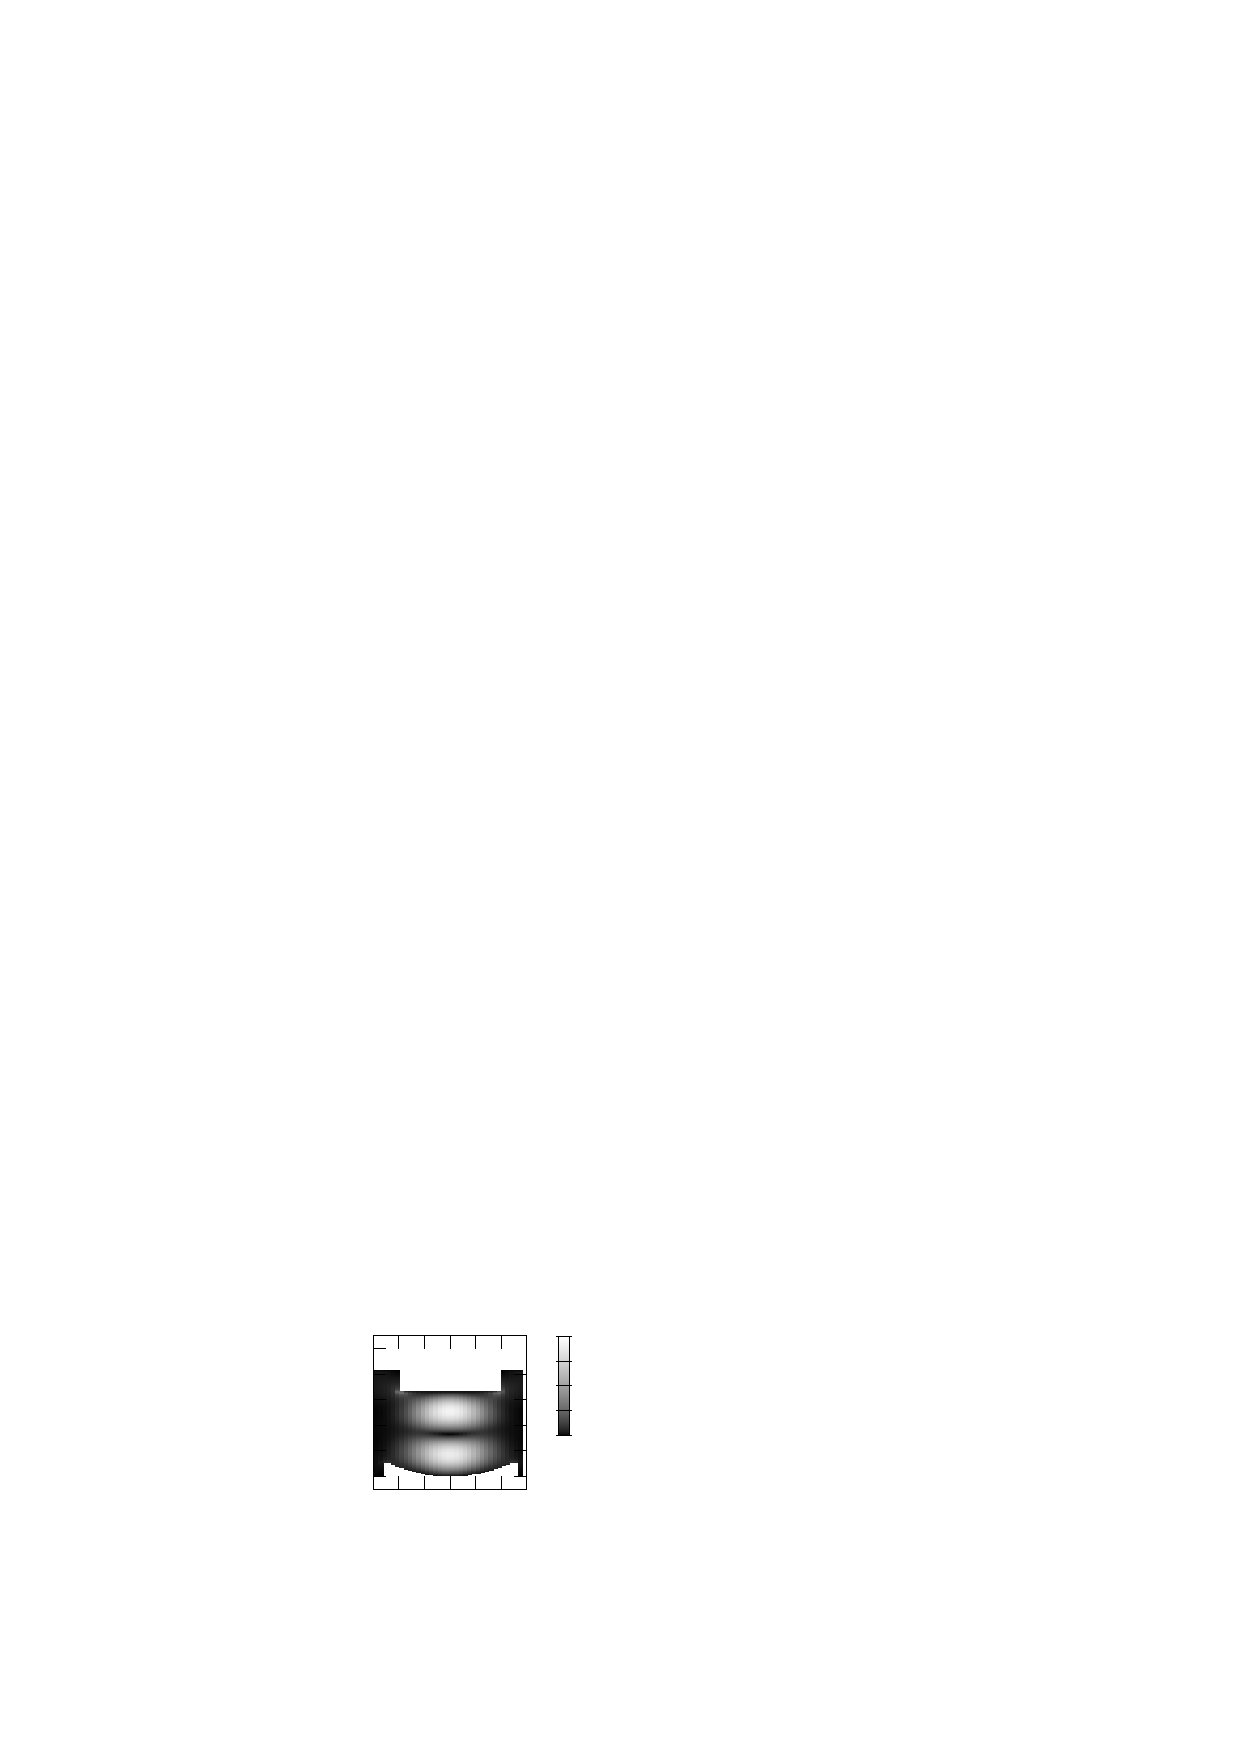
\includegraphics{variaciones-U}%
%\end{picture}%
%\begingroup
%\setlength{\unitlength}{0.0200bp}%
%\begin{picture}(14400,8640)(0,0)%
%\put(10336,4054){\makebox(0,0)[l]{\strut{}0.00}}%
%\put(10336,4646){\makebox(0,0)[l]{\strut{}0.25}}%
%\put(10336,5238){\makebox(0,0)[l]{\strut{}0.50}}%
%\put(10336,5830){\makebox(0,0)[l]{\strut{}0.75}}%
%\put(10336,6422){\makebox(0,0)[l]{\strut{}1.00}}%
%\put(9038,2206){\makebox(0,0){\strut{}-6}}%
%\put(8426,2206){\makebox(0,0){\strut{}-4}}%
%\put(7812,2206){\makebox(0,0){\strut{}-2}}%
%\put(7200,2206){\makebox(0,0){\strut{} 0}}%
%\put(6587,2206){\makebox(0,0){\strut{} 2}}%
%\put(5974,2206){\makebox(0,0){\strut{} 4}}%
%\put(5361,2206){\makebox(0,0){\strut{} 6}}%
%\put(5086,3063){\makebox(0,0)[r]{\strut{} 0}}%
%\put(5086,3676){\makebox(0,0)[r]{\strut{} 2}}%
%\put(5087,4289){\makebox(0,0)[r]{\strut{} 4}}%
%\put(5087,4901){\makebox(0,0)[r]{\strut{} 6}}%
%\put(5087,5514){\makebox(0,0)[r]{\strut{} 8}}%
%\put(5087,6127){\makebox(0,0)[r]{\strut{} 10}}%
%\put(7200,1206){\makebox(0,0){\strut{} $x^\ast$}}%
%\put(4087,4289){\makebox(0,0)[r]{\strut{} $y^\ast$}}%
%\put(7200,206){\makebox(0,0){\strut{} (a)}}%
%\end{picture}%
%\endgroup
%\endinput

\hskip -3.1cm
%GNUPLOT: LaTeX picture with Postscript
%\begin{picture}(0,0)%
%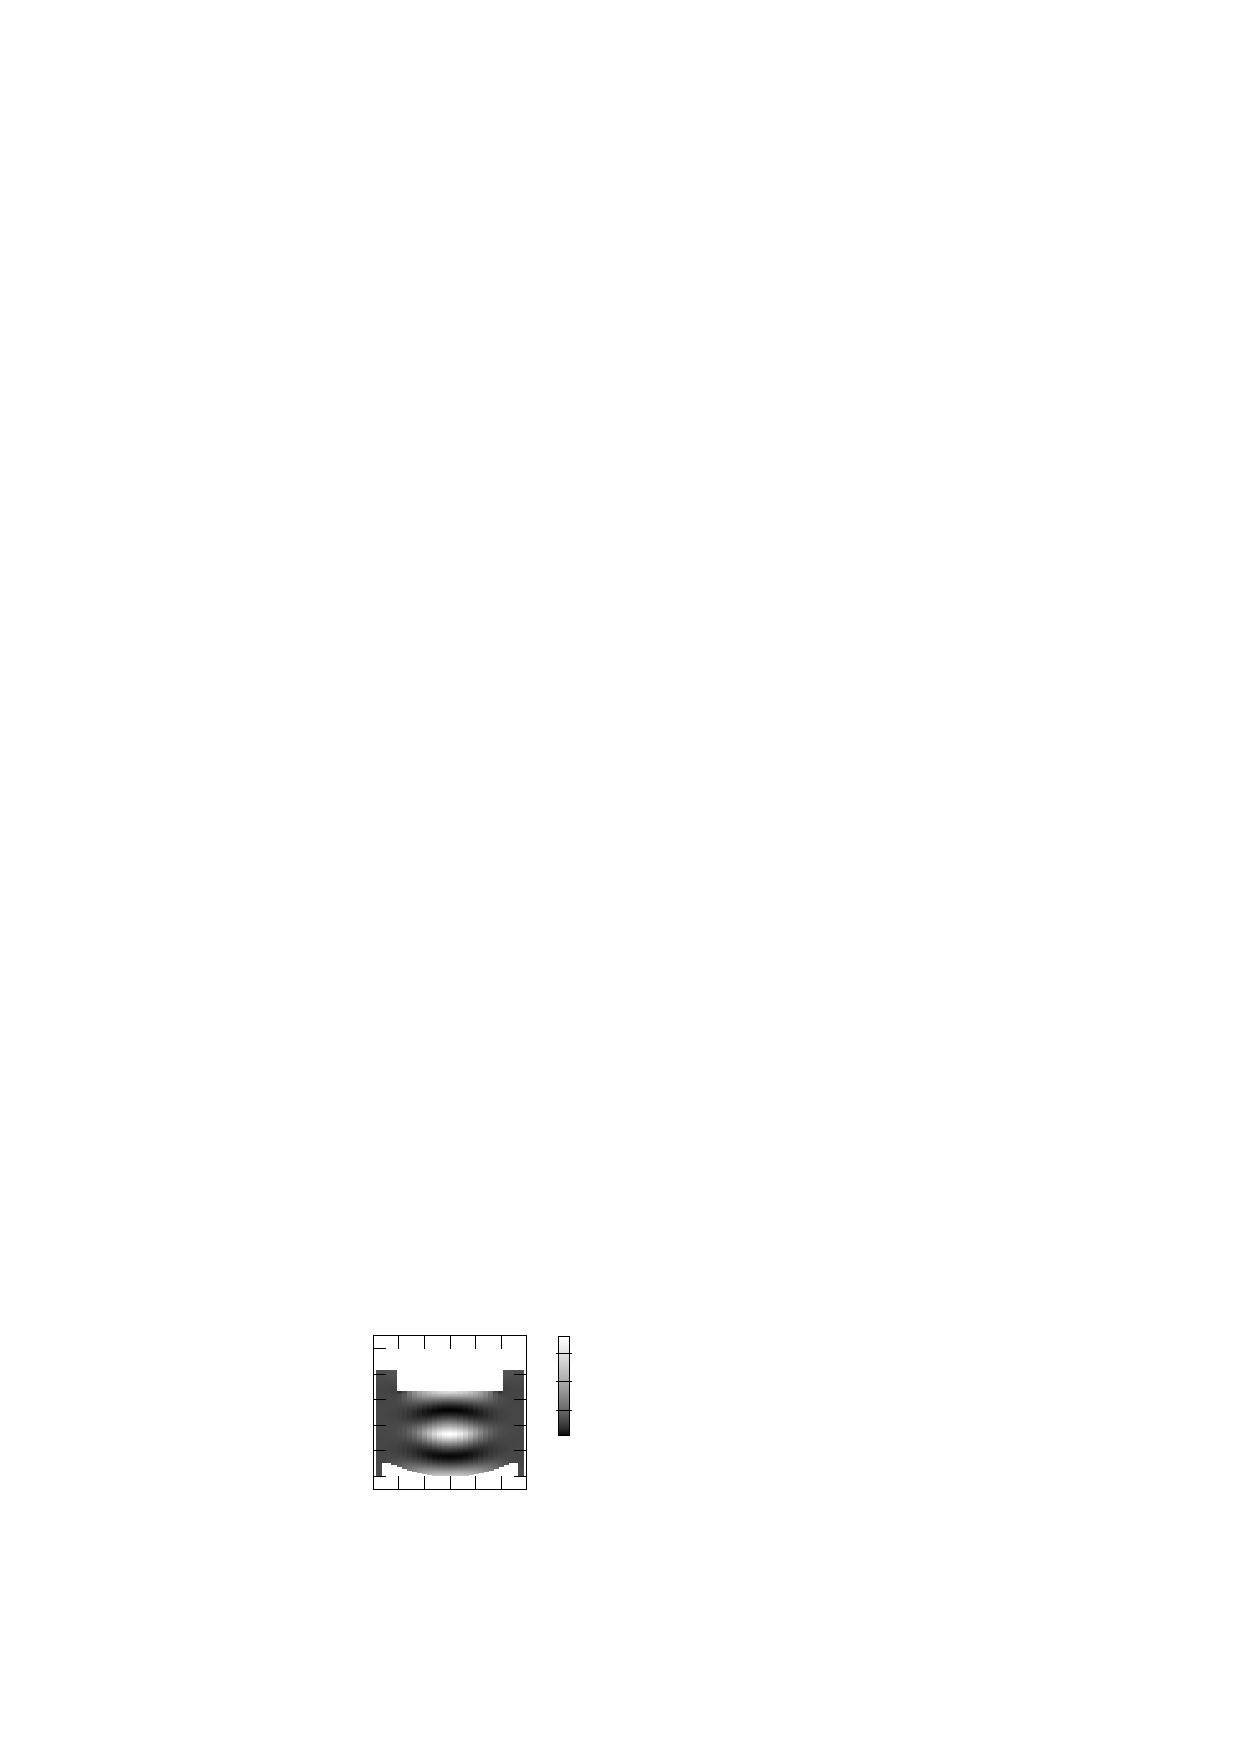
\includegraphics{variaciones-P}%
%\end{picture}%
%\begingroup
%\setlength{\unitlength}{0.0200bp}%
%\begin{picture}(14400,8640)(0,0)%
%\put(10336,4643){\makebox(0,0)[l]{\strut{}1.001}}%
%\put(10336,5329){\makebox(0,0)[l]{\strut{}1.003}}%
%\put(10336,6015){\makebox(0,0)[l]{\strut{}1.005}}%
%\put(9038,2206){\makebox(0,0){\strut{}-6}}%
%\put(8426,2206){\makebox(0,0){\strut{}-4}}%
%\put(7812,2206){\makebox(0,0){\strut{}-2}}%
%\put(7200,2206){\makebox(0,0){\strut{} 0}}%
%\put(6587,2206){\makebox(0,0){\strut{} 2}}%
%\put(5974,2206){\makebox(0,0){\strut{} 4}}%
%\put(5361,2206){\makebox(0,0){\strut{} 6}}%
%\put(5086,3063){\makebox(0,0)[r]{\strut{} 0}}%
%\put(5086,3676){\makebox(0,0)[r]{\strut{} 2}}%
%\put(5087,4289){\makebox(0,0)[r]{\strut{} 4}}%
%\put(5087,4901){\makebox(0,0)[r]{\strut{} 6}}%
%\put(5087,5514){\makebox(0,0)[r]{\strut{} 8}}%
%\put(5087,6127){\makebox(0,0)[r]{\strut{} 10}}%
%\put(7200,1206){\makebox(0,0){\strut{} $x^\ast$}}%
%\put(4087,4289){\makebox(0,0)[r]{\strut{} $y^\ast$}}%
%\put(7200,206){\makebox(0,0){\strut{} (b)}}%
%\end{picture}%
%\endgroup
%\endinput

\caption{\label{fig:nodos-presion-velocidad}
(a) Amplitud de la oscilaci'on de la velocidad escalada con la velocidad m'axima y (b) amplitud de oscilaci'on 
de la presi'on escalada con la presi'on inicial para la cavidad redondeada. 
La cantidad de movimiento agregado por la fuente ac'ustica es 
$P_o^\ast = 1.6 \times 10^{-3}$. La  frecuencia  de la fuente ac'ustica es $\omega_r = 0.019126$ para la cavidad
redondeada  correspondiente al segundo modo resonante.
}
\end{figure}


Todas las simulaciones num'ericas que reportamos en esta secci'on corresponden al segundo modo resonante. 
La cavidad plana se inicializa con una onda estacionaria plana con una frecuencia correspondiente al 
segundo modo resonante. En la cavidad redondeada, dada la geometr'ia del reflector redondeado, 
partimos de un sistema en reposo y dejamos evolucionar hasta 
formar una onda estacionaria en  aproximadamente 400 periodos.
En las figuras~\ref{fig:nodos-presion-velocidad} (a) y (b) mostramos los mapas de la amplitud de la oscilaci'on 
local para la velocidad y la presi'on en la cavidad redondeada, respectivamente. 
De estas figuras observamos que a un nodo de presi'on le corresponde un antinodo de velocidad, o escrito
de otra forma, en un lugar donde la amplitud de oscilaci'on de la presi'on es cero, la amplitud de oscilaci'on 
de la velocidad es m'axima y viceversa.

En el primer conjunto de simulaciones num'ericas en presencia de part'icula s'olida,
colocamos una part'icula  libre de moverse de radio $r^\ast =0.25$  a diferentes alturas en el eje vertical de
ambas cavidades y monitoreamos el movimiento vertical y horizontal de la part'icula.  
En las figuras~\ref{fig:y-g-0} (a) y (b) reportamos la posici'on vertical de una part'icula variando
su posici'on inicial en ausencia de gravedad. En la cavidad redondeada, la posici'on horizontal inicial
est'a en el eje vertical. Para los valores de los par'ametros usados en estas simulaciones, no 
hay movimiento de la part'icula en el eje horizontal.
Como trabajamos en el segundo modo resonante, existen dos nodos de presi'on,
y las part'iculas colocadas dentro de las cavidades se mueven hacia los nodo de presi'on m'as cercanos
que se encuentran en $y^\ast = 1.6$ y $y^\ast = $ para la cavida plana y $y^\ast =1.45$ y $y^\ast =5.3$ para la
cavidad redondeada , donde la sumatoria de fuerzas ac'usticas es cero. Al comparar el movimiento de las part'iculas en ambas cavidades,
podemos concluir que las que se encuentran en la cavidad redondeada alcanzan el nodo de presi'on en un tiempo
menor que las colocadas en la cavidad plana.
En ambas cavidades, la part'icula oscila alrededor del nodo de presi'on como enfatizamos en la 
figura~\ref{fig:detalle-flat-rounded} y las frecuencias de oscilaci'on coinciden con la frecuencia de la fuente ac'ustica.
Tambi'en observamos que el movimiento de la part'icula en la cavidad redondeada presenta arm'onicos
de la frecuencia de la fuente ac'ustica, los cuales no aparecen para la part'icula en la cavidad plana
\begin{figure} 
%\put(7650,9588){\makebox(0,0)[r]{\strut{} (a)}}%
%%GNUPLOT: LaTeX picture with Postscript
%\begin{picture}(0,0)%
%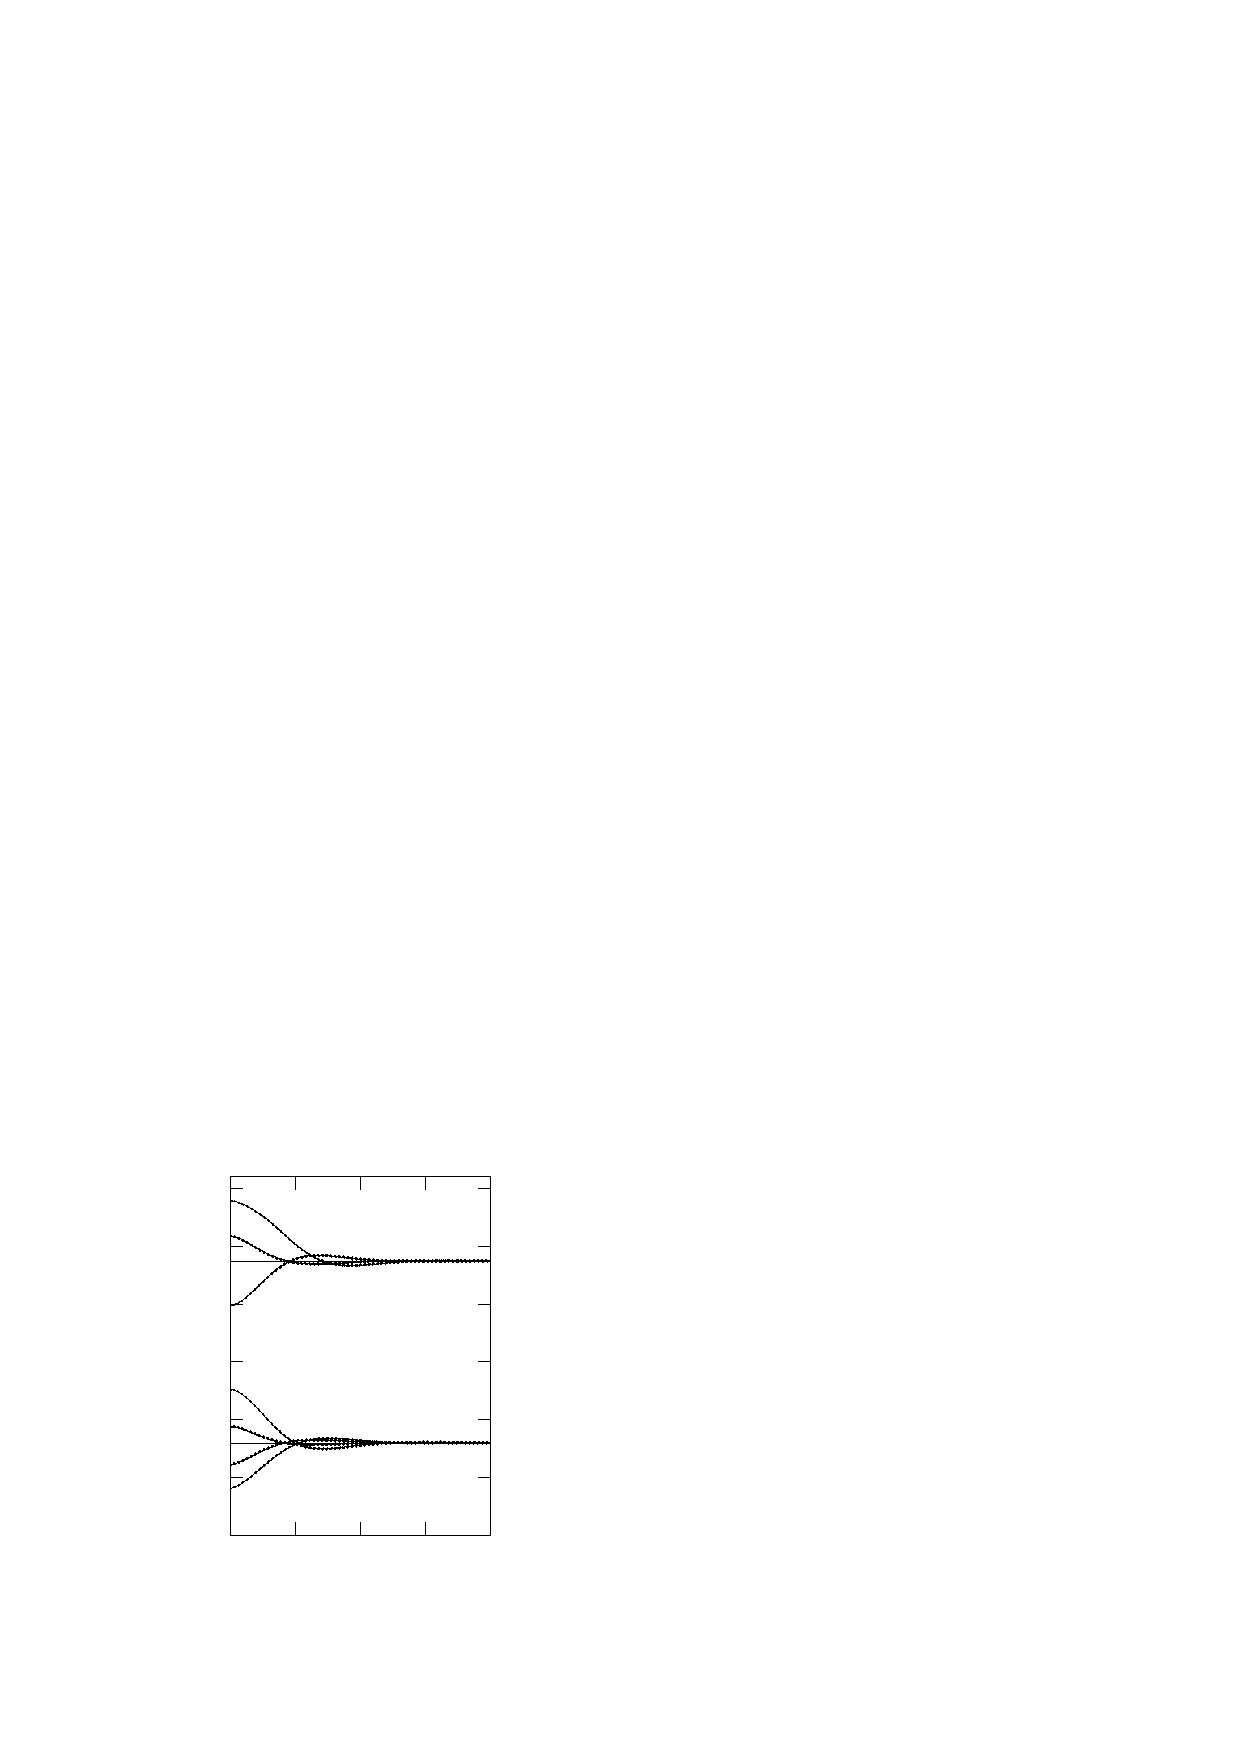
\includegraphics{position-flat-zerogravity}%
%\end{picture}%
%\begingroup
%\setlength{\unitlength}{0.0200bp}%
%\begin{picture}(9000,10800)(0,0)%
%\put(1650,1650){\makebox(0,0)[r]{\strut{} 0}}%
%\put(1650,3037){\makebox(0,0)[r]{\strut{} 1}}%
%\put(1650,4424){\makebox(0,0)[r]{\strut{} 2}}%
%\put(1650,5811){\makebox(0,0)[r]{\strut{} 3}}%
%\put(1650,7198){\makebox(0,0)[r]{\strut{} 4}}%
%\put(1650,8585){\makebox(0,0)[r]{\strut{} 5}}%
%\put(1650,9973){\makebox(0,0)[r]{\strut{} 6}}%
%\put(1925,1100){\makebox(0,0){\strut{} 0}}%
%\put(3488,1100){\makebox(0,0){\strut{} 50}}%
%\put(5050,1100){\makebox(0,0){\strut{} 100}}%
%\put(6613,1100){\makebox(0,0){\strut{} 150}}%
%\put(8175,1100){\makebox(0,0){\strut{} 200}}%
%\put(550,5950){\rotatebox{90}{\makebox(0,0){\strut{}$y^\ast$}}}%
%\put(5050,275){\makebox(0,0){\strut{}$t^\ast$}}%
%\put(7650,9588){\makebox(0,0)[r]{\strut{} (a)}}%
%\end{picture}%
%\endgroup
%\endinput

%GNUPLOT: LaTeX picture with Postscript
\begin{picture}(0,0)%
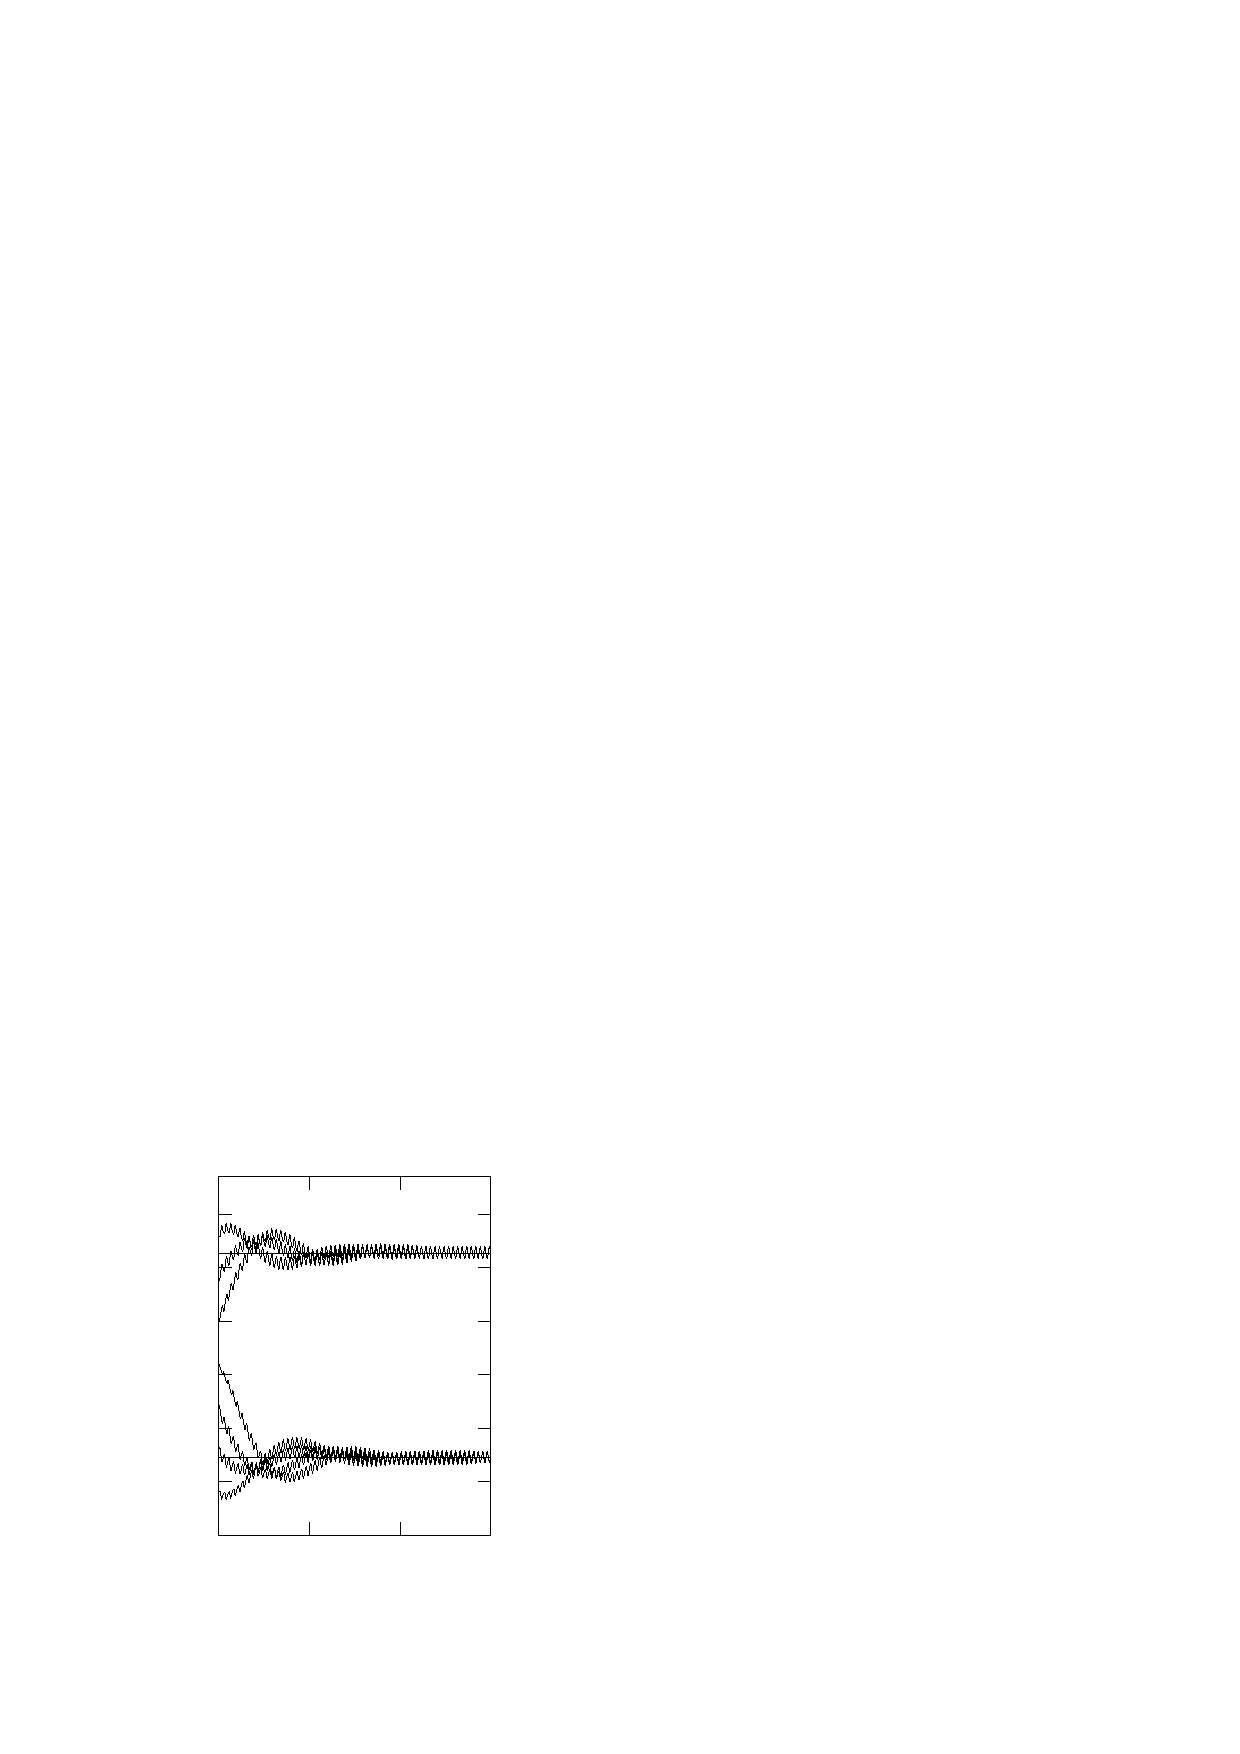
\includegraphics{eps/position-rounded-zerogravity}%
\end{picture}%
\begingroup
\setlength{\unitlength}{0.0200bp}%
\begin{picture}(9000,10800)(0,0)%
\put(1375,1650){\makebox(0,0)[r]{\strut{}0}}%
\put(1375,2934){\makebox(0,0)[r]{\strut{}1}}%
\put(1375,4217){\makebox(0,0)[r]{\strut{}2}}%
\put(1375,5501){\makebox(0,0)[r]{\strut{}3}}%
\put(1375,6784){\makebox(0,0)[r]{\strut{}4}}%
\put(1375,8068){\makebox(0,0)[r]{\strut{}5}}%
\put(1375,9351){\makebox(0,0)[r]{\strut{}6}}%
\put(1650,1100){\makebox(0,0){\strut{} 0}}%
\put(3825,1100){\makebox(0,0){\strut{} 20}}%
\put(6000,1100){\makebox(0,0){\strut{} 40}}%
\put(8175,1100){\makebox(0,0){\strut{} 60}}%
\put(550,5950){\rotatebox{90}{\makebox(0,0){\strut{}$y^\ast$}}}%
\put(4912,275){\makebox(0,0){\strut{}$t^\ast$}}%

\put(7650,9588){\makebox(0,0)[r]{\strut{} (b)}}%

\end{picture}%
\endgroup
\endinput

\vskip 5mm
\caption{\label{fig:y-g-0}
Evoluci'on de la posici'on vertical de una part'icula s'olida como funci'on del tiempo
en el segundo modo resonante en ausencia de gravedad en (a) la cavidad  plana y (b) la
cavidad  redondeada, ambas con  $P_o^\ast = 1.6\times 10^{-3}$, $\rho_p/\rho_f=2$, y $r^\ast=0.25$.
Las l'ineas horizontales representan la ubicaci'on de los nodos de presi'on. 
}
\end{figure}
\begin{figure} 
%GNUPLOT: LaTeX picture with Postscript
%\begin{picture}(0,0)%
%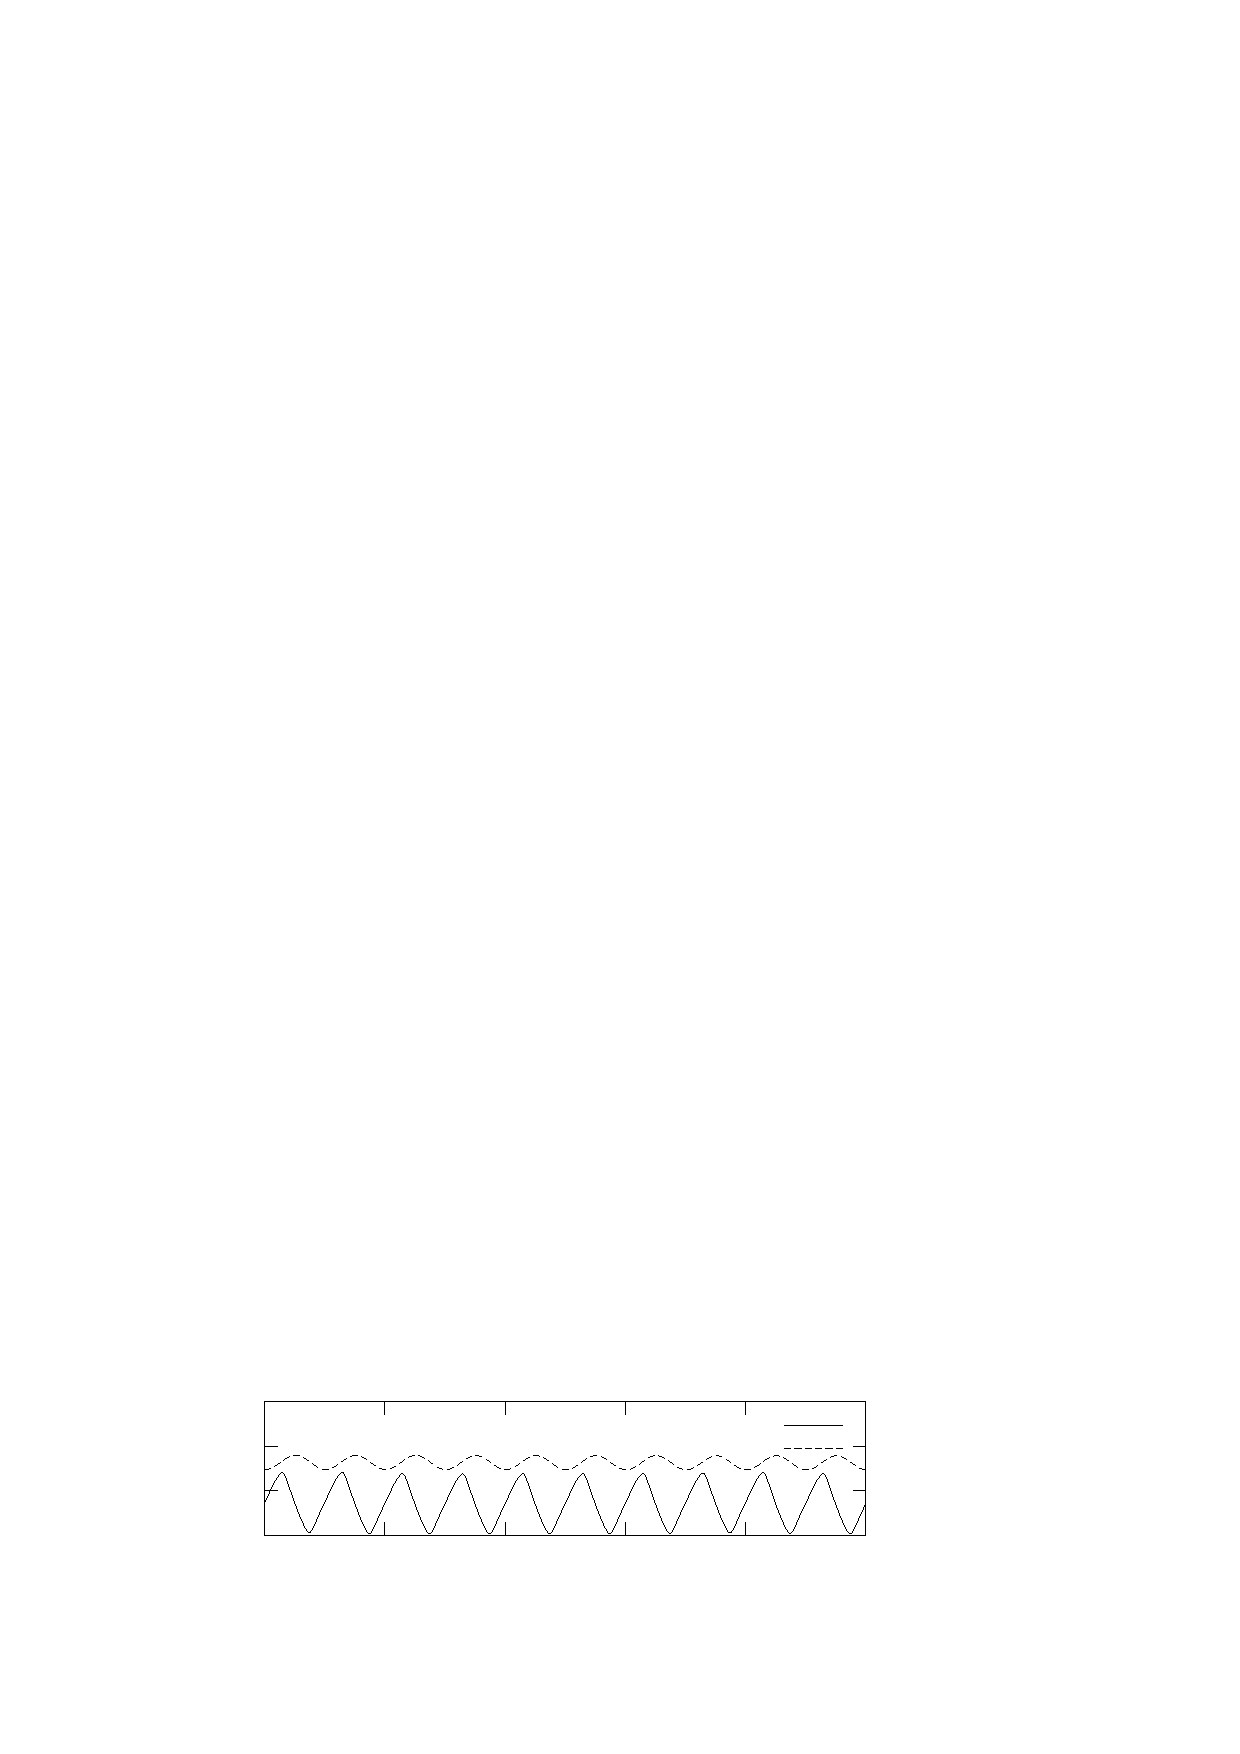
\includegraphics{detalle-rounded-flat-zerogravity}%
%\end{picture}%
%\begingroup
%\setlength{\unitlength}{0.0200bp}%
%\begin{picture}(18000,5400)(0,0)%
%\put(2475,1650){\makebox(0,0)[r]{\strut{} 1.35}}%
%\put(2475,2717){\makebox(0,0)[r]{\strut{} 1.50}}%
%\put(2475,3783){\makebox(0,0)[r]{\strut{} 1.65}}%
%\put(2475,4850){\makebox(0,0)[r]{\strut{} 1.80}}%
%\put(2750,1100){\makebox(0,0){\strut{} 120}}%
%\put(5635,1100){\makebox(0,0){\strut{} 122}}%
%\put(8520,1100){\makebox(0,0){\strut{} 124}}%
%\put(11405,1100){\makebox(0,0){\strut{} 126}}%
%\put(14290,1100){\makebox(0,0){\strut{} 128}}%
%\put(17175,1100){\makebox(0,0){\strut{} 130}}%
%\put(550,3250){\rotatebox{90}{\makebox(0,0){\strut{}$y^\ast$}}}%
%\put(9962,275){\makebox(0,0){\strut{}$t^\ast$}}%
%%\put(600,1000){\rotatebox{0}{\makebox(0,0){\strut{}(a)}}}%
%\put(14950,4275){\makebox(0,0)[r]{\strut{}redondeada}}%
%\put(14950,3725){\makebox(0,0)[r]{\strut{}plana}}%
%\end{picture}%
%\endgroup
%\endinput

%%GNUPLOT: LaTeX picture with Postscript
\begin{picture}(0,0)%
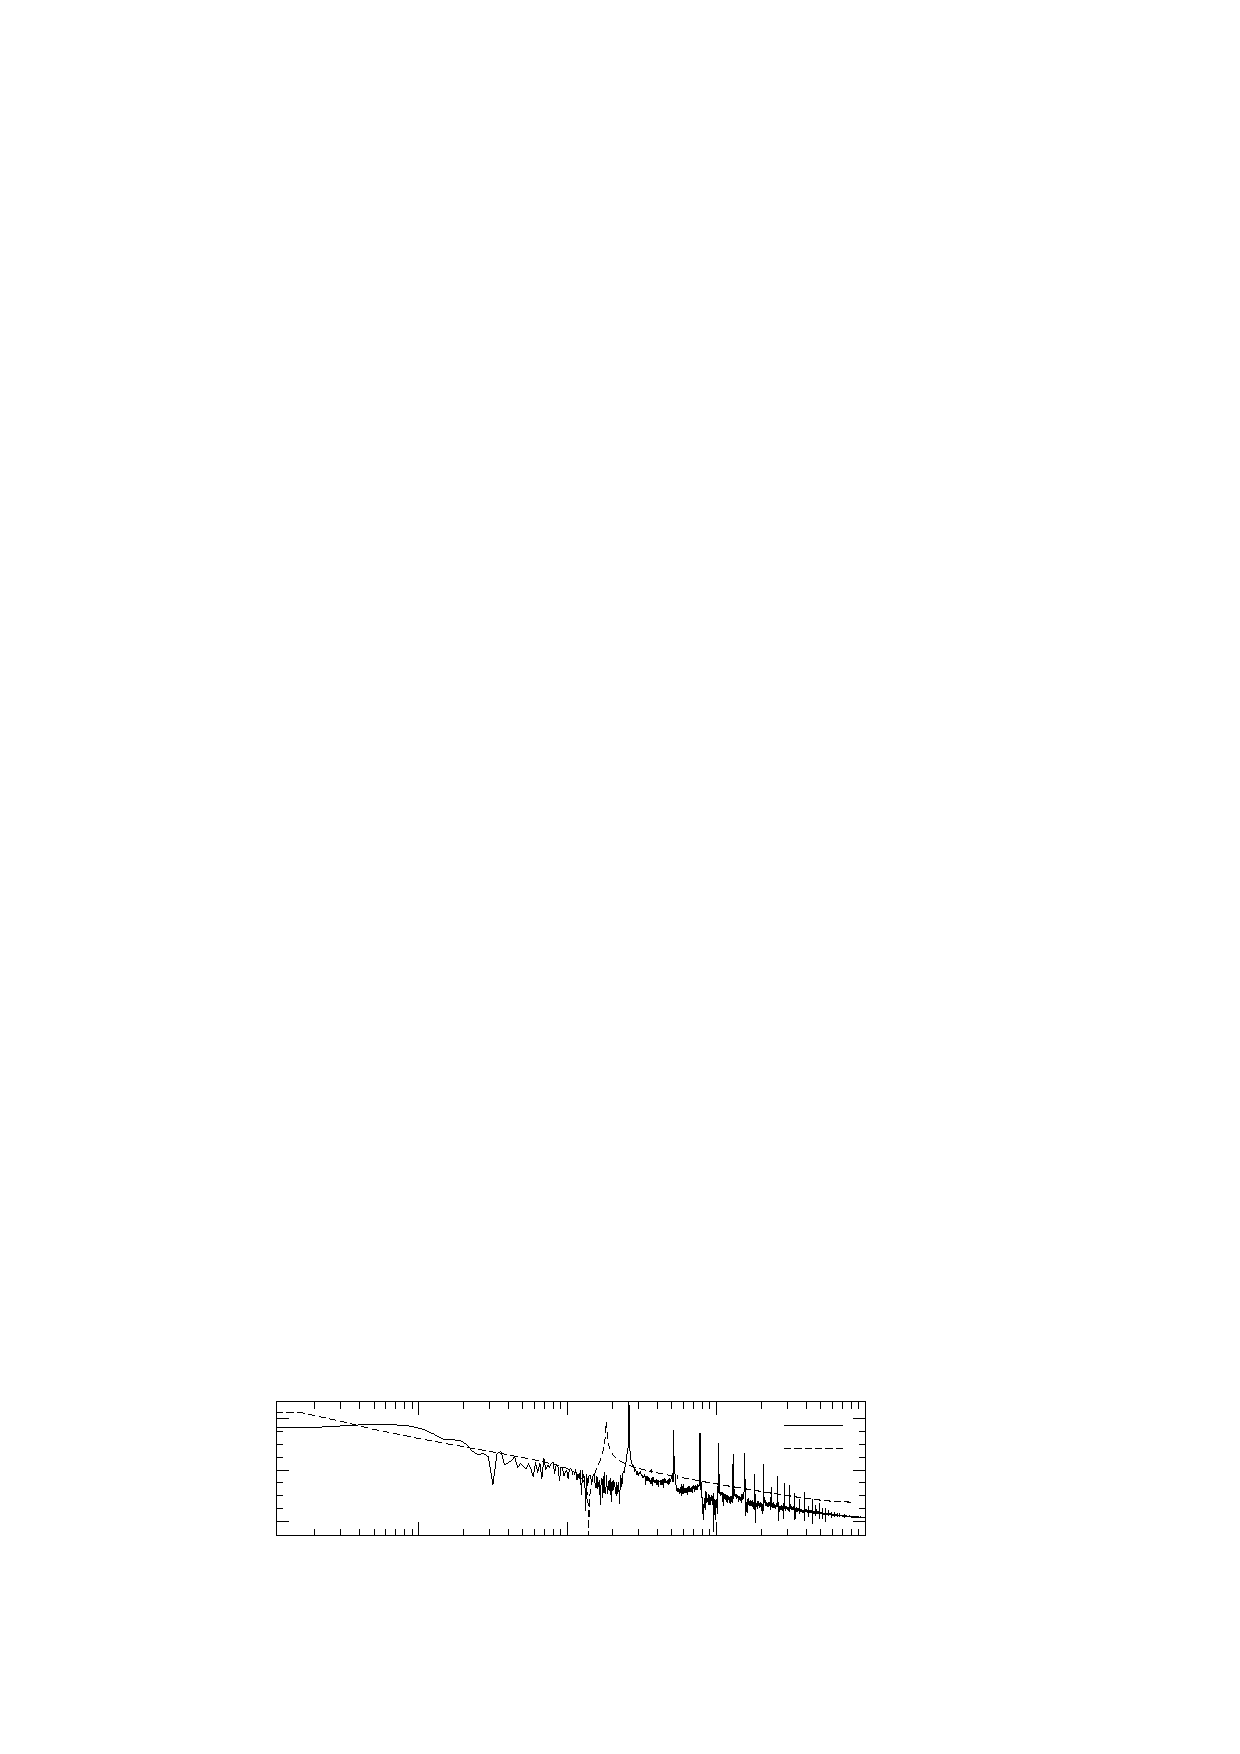
\includegraphics{detalle-frecuencias-rounded-flat}%
\end{picture}%
\begingroup
\setlength{\unitlength}{0.0200bp}%
\begin{picture}(18000,5400)(0,0)%
\put(2750,1987){\makebox(0,0)[r]{\strut{} 1e-12}}%
\put(2750,3214){\makebox(0,0)[r]{\strut{} 1e-08}}%
\put(2750,4441){\makebox(0,0)[r]{\strut{} 1e-04}}%
\put(6452,1100){\makebox(0,0){\strut{} 0.001}}%
\put(10026,1100){\makebox(0,0){\strut{} 0.01}}%
\put(13601,1100){\makebox(0,0){\strut{} 0.1}}%
\put(17175,1100){\makebox(0,0){\strut{} 1}}%
\put(550,3250){\rotatebox{90}{\makebox(0,0){\strut{}$PSD$}}}%
\put(10100,275){\makebox(0,0){\strut{}$\omega$}}%
\put(14950,4275){\makebox(0,0)[r]{\strut{}redondeada}}%
\put(14950,3725){\makebox(0,0)[r]{\strut{}plana}}%
\put(600,1000){\rotatebox{0}{\makebox(0,0){\strut{}(b)}}}%
\end{picture}%
\endgroup
\endinput

\caption{\label{fig:detalle-flat-rounded}
Posici'on vertical de la part'icula para  la cavidad
plana y la redondeada. Ambas part'iculas oscilan con una frecuencia correspondiente
a la de la fuente ac'ustica.
}
\end{figure}.

\begin{figure} 
%GNUPLOT: LaTeX picture with Postscript
\begin{picture}(0,0)%
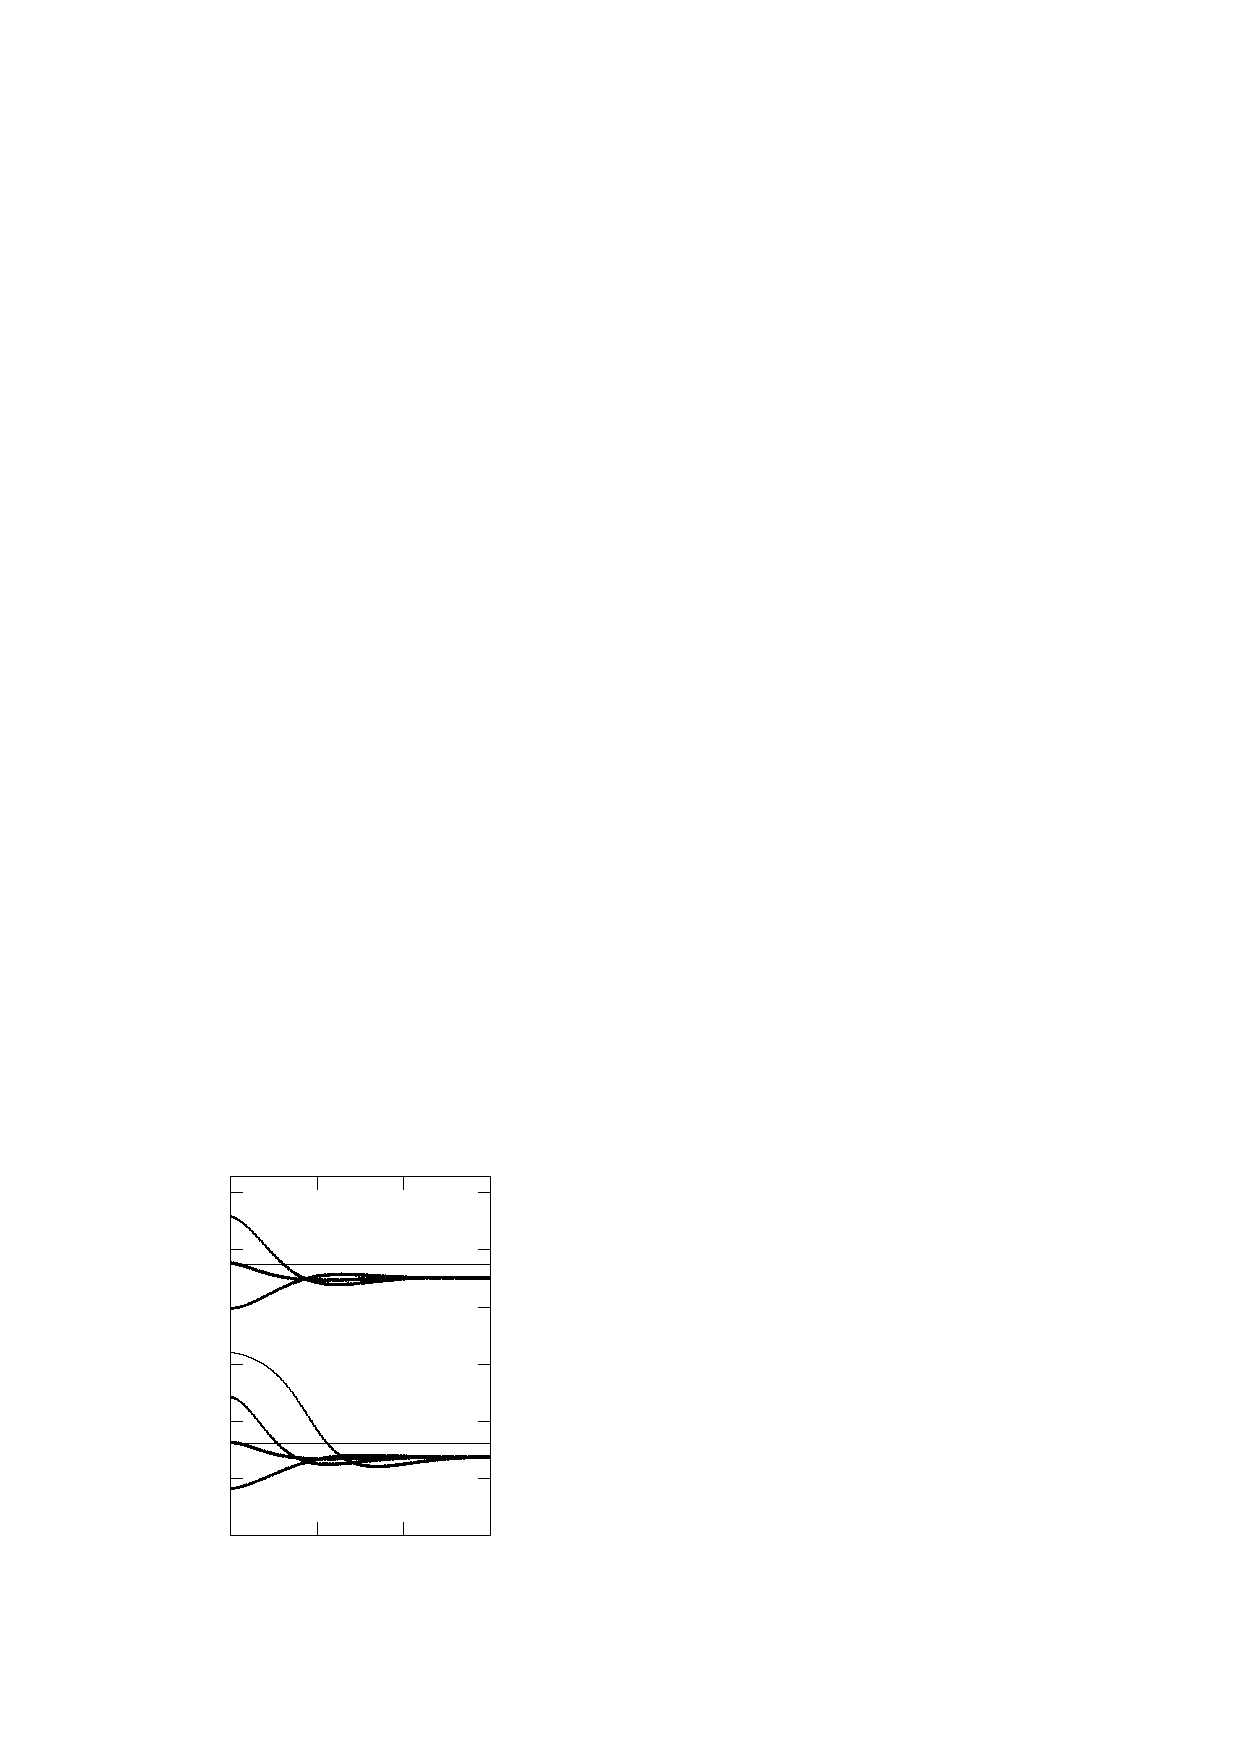
\includegraphics{eps/position-flat-nonzerogravity}%
\end{picture}%
\begingroup
\setlength{\unitlength}{0.0200bp}%
\begin{picture}(9000,10800)(0,0)%
\put(1650,1650){\makebox(0,0)[r]{\strut{} 0}}%
\put(1650,3019){\makebox(0,0)[r]{\strut{} 1}}%
\put(1650,4389){\makebox(0,0)[r]{\strut{} 2}}%
\put(1650,5758){\makebox(0,0)[r]{\strut{} 3}}%
\put(1650,7128){\makebox(0,0)[r]{\strut{} 4}}%
\put(1650,8497){\makebox(0,0)[r]{\strut{} 5}}%
\put(1650,9867){\makebox(0,0)[r]{\strut{} 6}}%
\put(1925,1100){\makebox(0,0){\strut{} 0}}%
\put(4008,1100){\makebox(0,0){\strut{} 60}}%
\put(6092,1100){\makebox(0,0){\strut{} 120}}%
\put(8175,1100){\makebox(0,0){\strut{} 180}}%
\put(550,5950){\rotatebox{90}{\makebox(0,0){\strut{}$y^\ast$}}}%
\put(5050,275){\makebox(0,0){\strut{}$t^\ast$}}%

\put(7650,9588){\makebox(0,0)[r]{\strut{} (a)}}%
\end{picture}%
\endgroup
\endinput

%GNUPLOT: LaTeX picture with Postscript
\begin{picture}(0,0)%
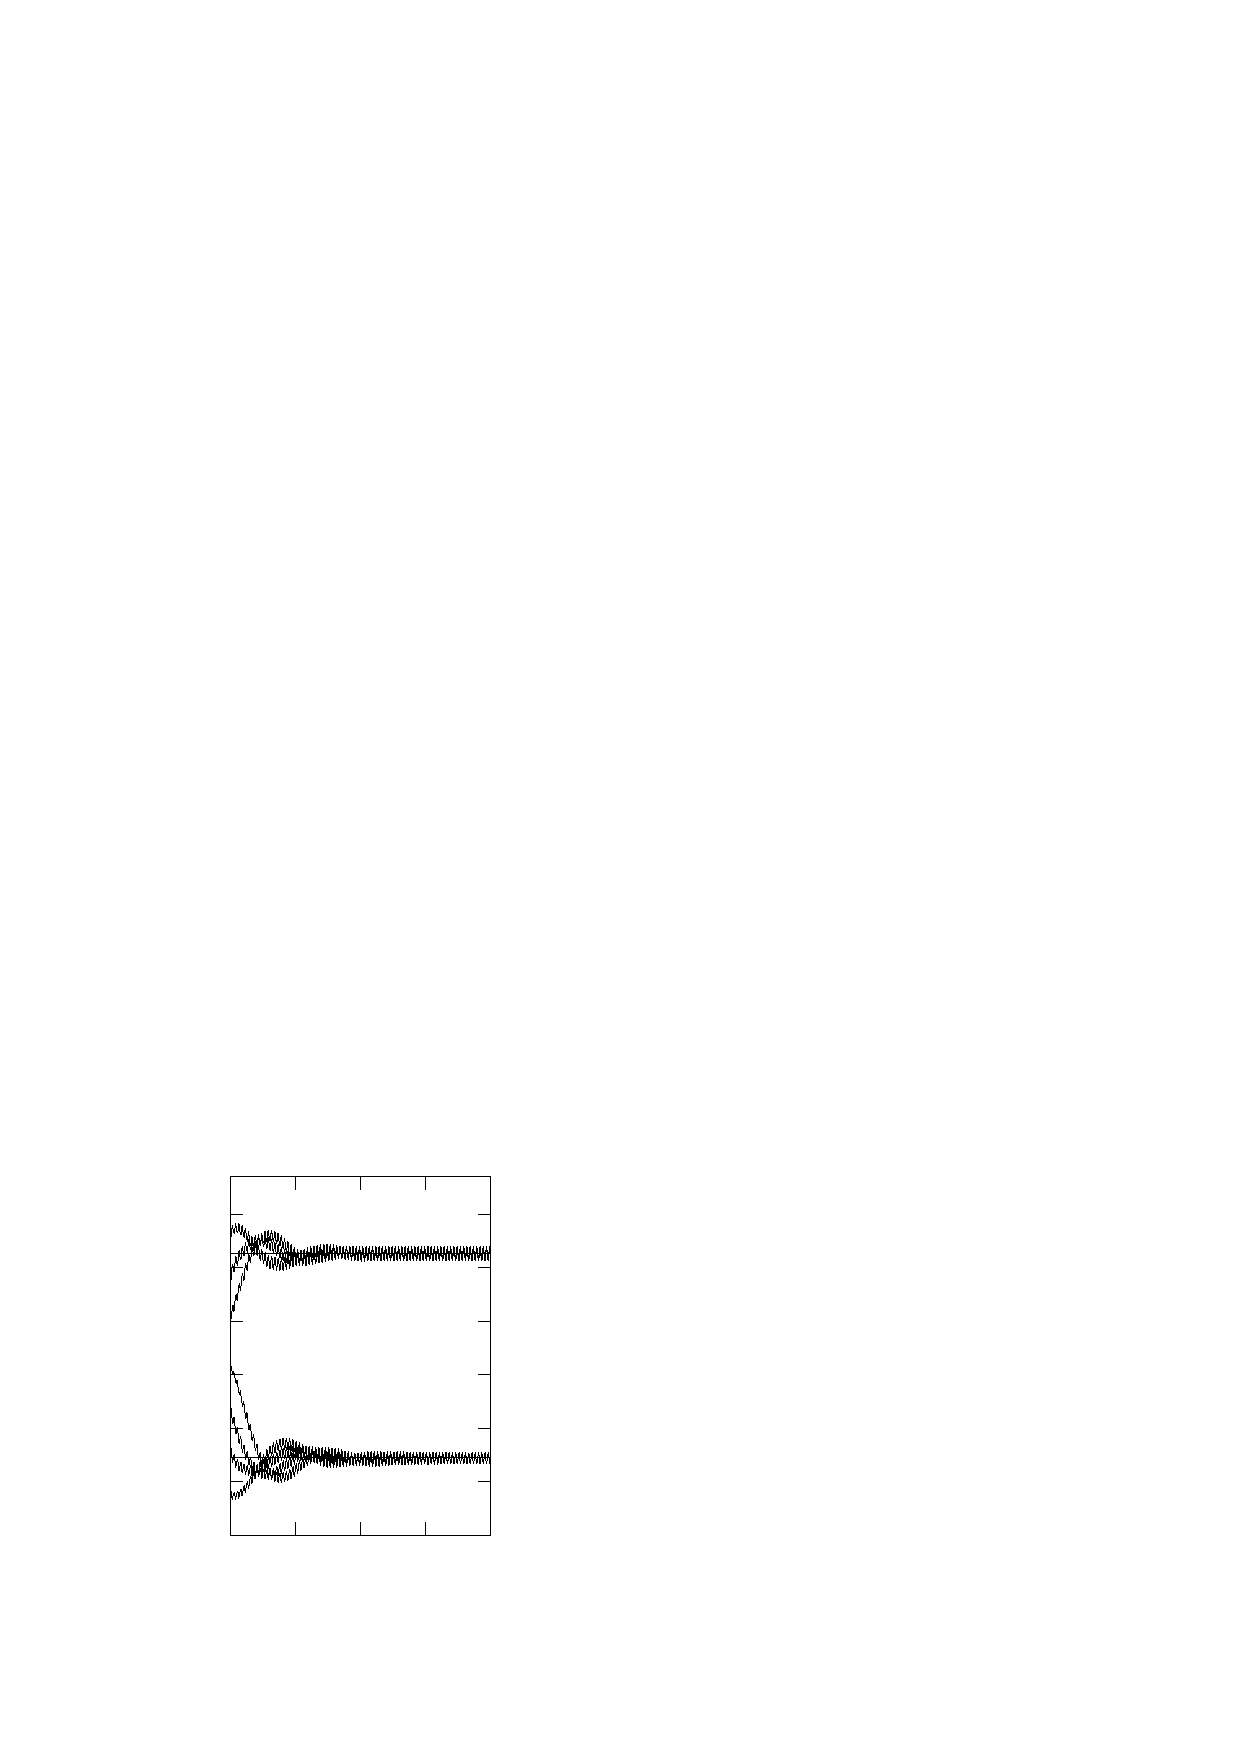
\includegraphics{eps/position-rounded-nonzerogravity}%
\end{picture}%
\begingroup
\setlength{\unitlength}{0.0200bp}%
\begin{picture}(9000,10800)(0,0)%
\put(1650,1650){\makebox(0,0)[r]{\strut{} 0}}%
\put(1650,2934){\makebox(0,0)[r]{\strut{} 1}}%
\put(1650,4217){\makebox(0,0)[r]{\strut{} 2}}%
\put(1650,5501){\makebox(0,0)[r]{\strut{} 3}}%
\put(1650,6784){\makebox(0,0)[r]{\strut{} 4}}%
\put(1650,8068){\makebox(0,0)[r]{\strut{} 5}}%
\put(1650,9351){\makebox(0,0)[r]{\strut{} 6}}%
\put(1925,1100){\makebox(0,0){\strut{} 0}}%
\put(3488,1100){\makebox(0,0){\strut{} 20}}%
\put(5050,1100){\makebox(0,0){\strut{} 40}}%
\put(6613,1100){\makebox(0,0){\strut{} 60}}%
\put(8175,1100){\makebox(0,0){\strut{} 80}}%
\put(550,5950){\rotatebox{90}{\makebox(0,0){\strut{}$y^\ast$}}}%
\put(5050,275){\makebox(0,0){\strut{}$t^\ast$}}%

\put(7650,9588){\makebox(0,0)[r]{\strut{} (b)}}%

\end{picture}%
\endgroup
\endinput

\vskip 5mm
\caption{\label{fig:path-3} 
Evoluci'on de la posici'on vertical de una part'icula s'olida como funci'on del tiempo
en el segundo modo resonante en presencia de gravedad en (a) la cavidad  plana y (b) la
cavidad  redondeada. Las simulaciones num'ericas se realizaron con los mismos par'ametros 
de las figuras~\ref{fig:y-g-0} (a), (b) y agregando la presencia de un campo gravitacional externo.
}
\end{figure}
\begin{figure} 
%GNUPLOT: LaTeX picture with Postscript
%\begin{picture}(0,0)%
%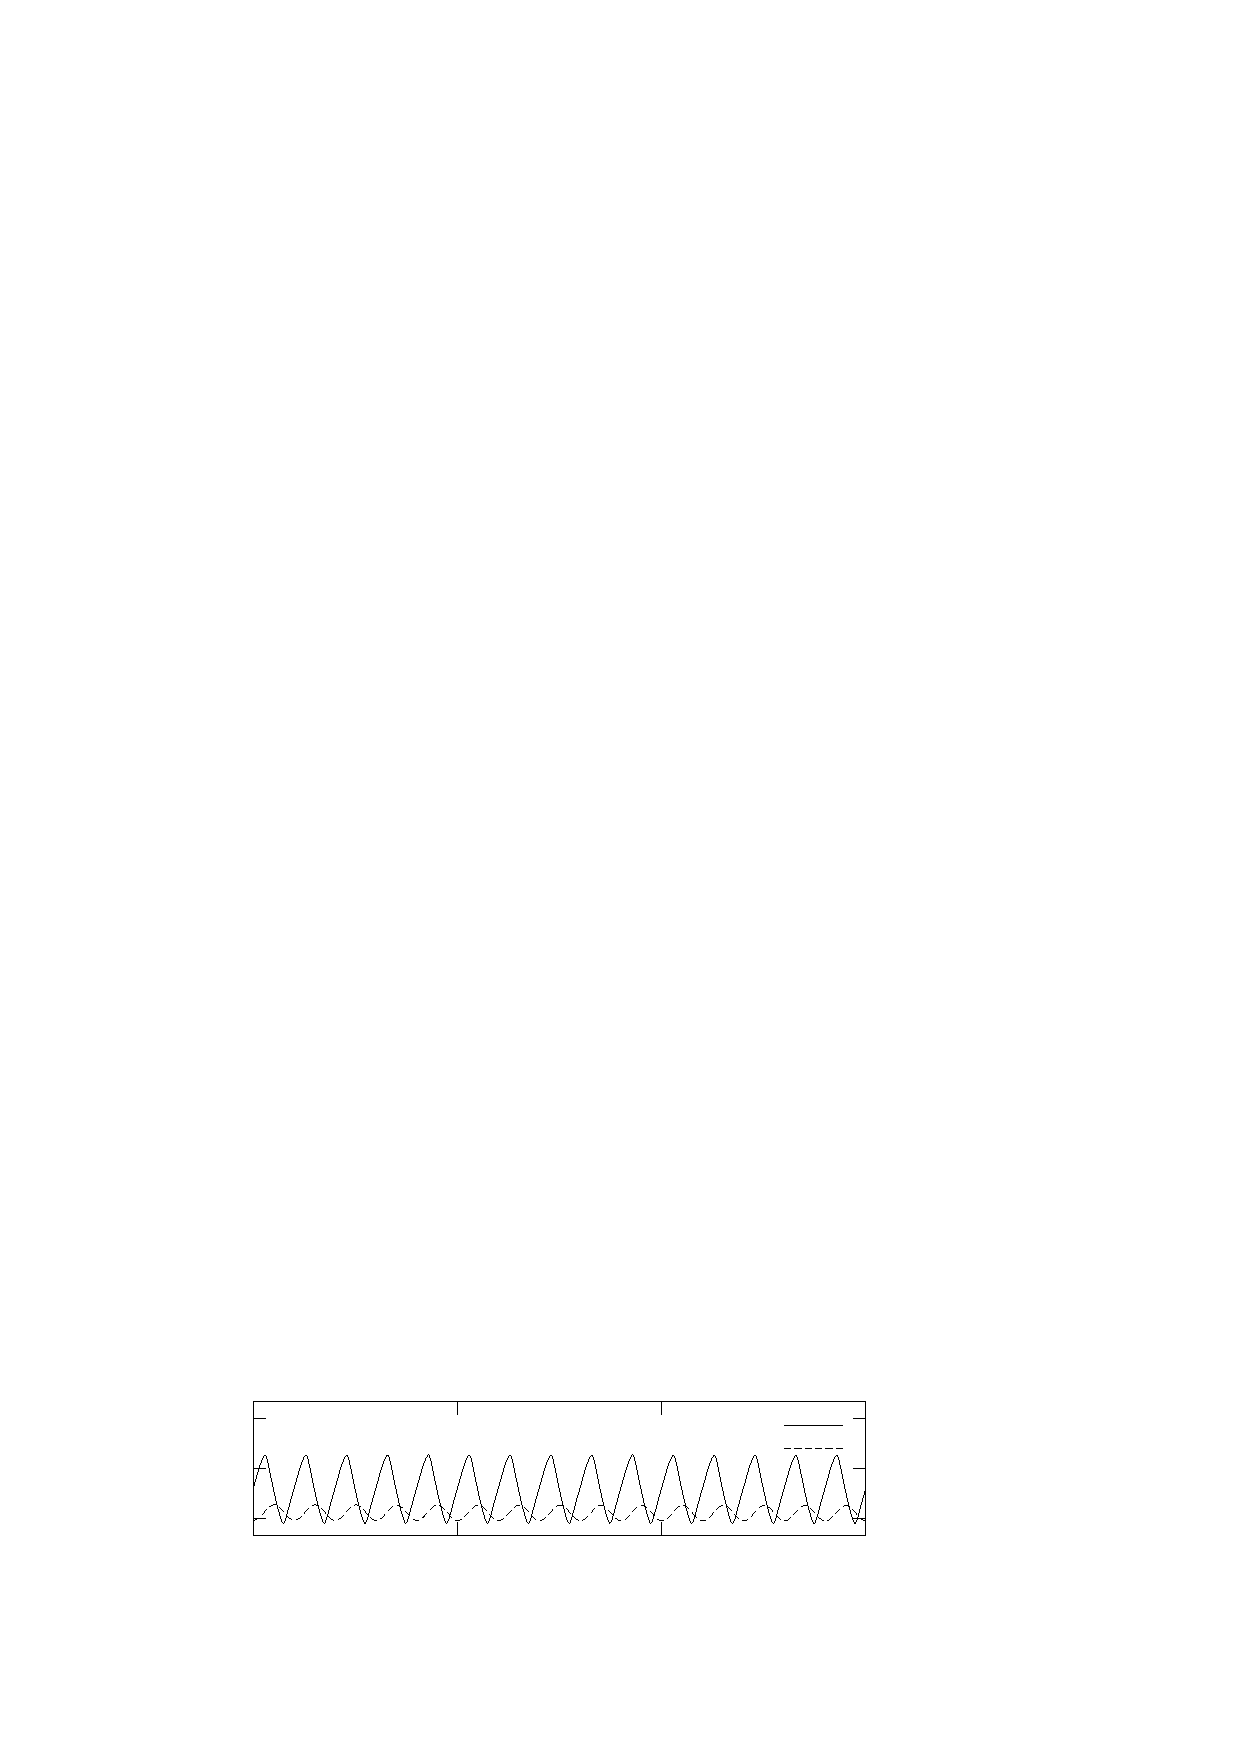
\includegraphics{detalle-rounded-flat-gravity}%
%\end{picture}%
%\begingroup
%\setlength{\unitlength}{0.0200bp}%
%\begin{picture}(18000,5400)(0,0)%
%\put(2200,2050){\makebox(0,0)[r]{\strut{}1.35}}%
%\put(2200,3250){\makebox(0,0)[r]{\strut{}1.50}}%
%\put(2200,4450){\makebox(0,0)[r]{\strut{}1.65}}%
%\put(2475,1100){\makebox(0,0){\strut{} 260}}%
%\put(7375,1100){\makebox(0,0){\strut{} 265}}%
%\put(12275,1100){\makebox(0,0){\strut{} 270}}%
%\put(17175,1100){\makebox(0,0){\strut{} 275}}%
%\put(550,3250){\rotatebox{90}{\makebox(0,0){\strut{}$y^\ast$}}}%
%\put(9825,275){\makebox(0,0){\strut{}$t^\ast$}}%
%\put(14950,4275){\makebox(0,0)[r]{\strut{}redondeada}}%
%\put(14950,3725){\makebox(0,0)[r]{\strut{}plana}}%
%%\put(600,1000){\rotatebox{0}{\makebox(0,0){\strut{}(a)}}}%
%\end{picture}%
%\endgroup
%\endinput

%%GNUPLOT: LaTeX picture with Postscript
\begin{picture}(0,0)%
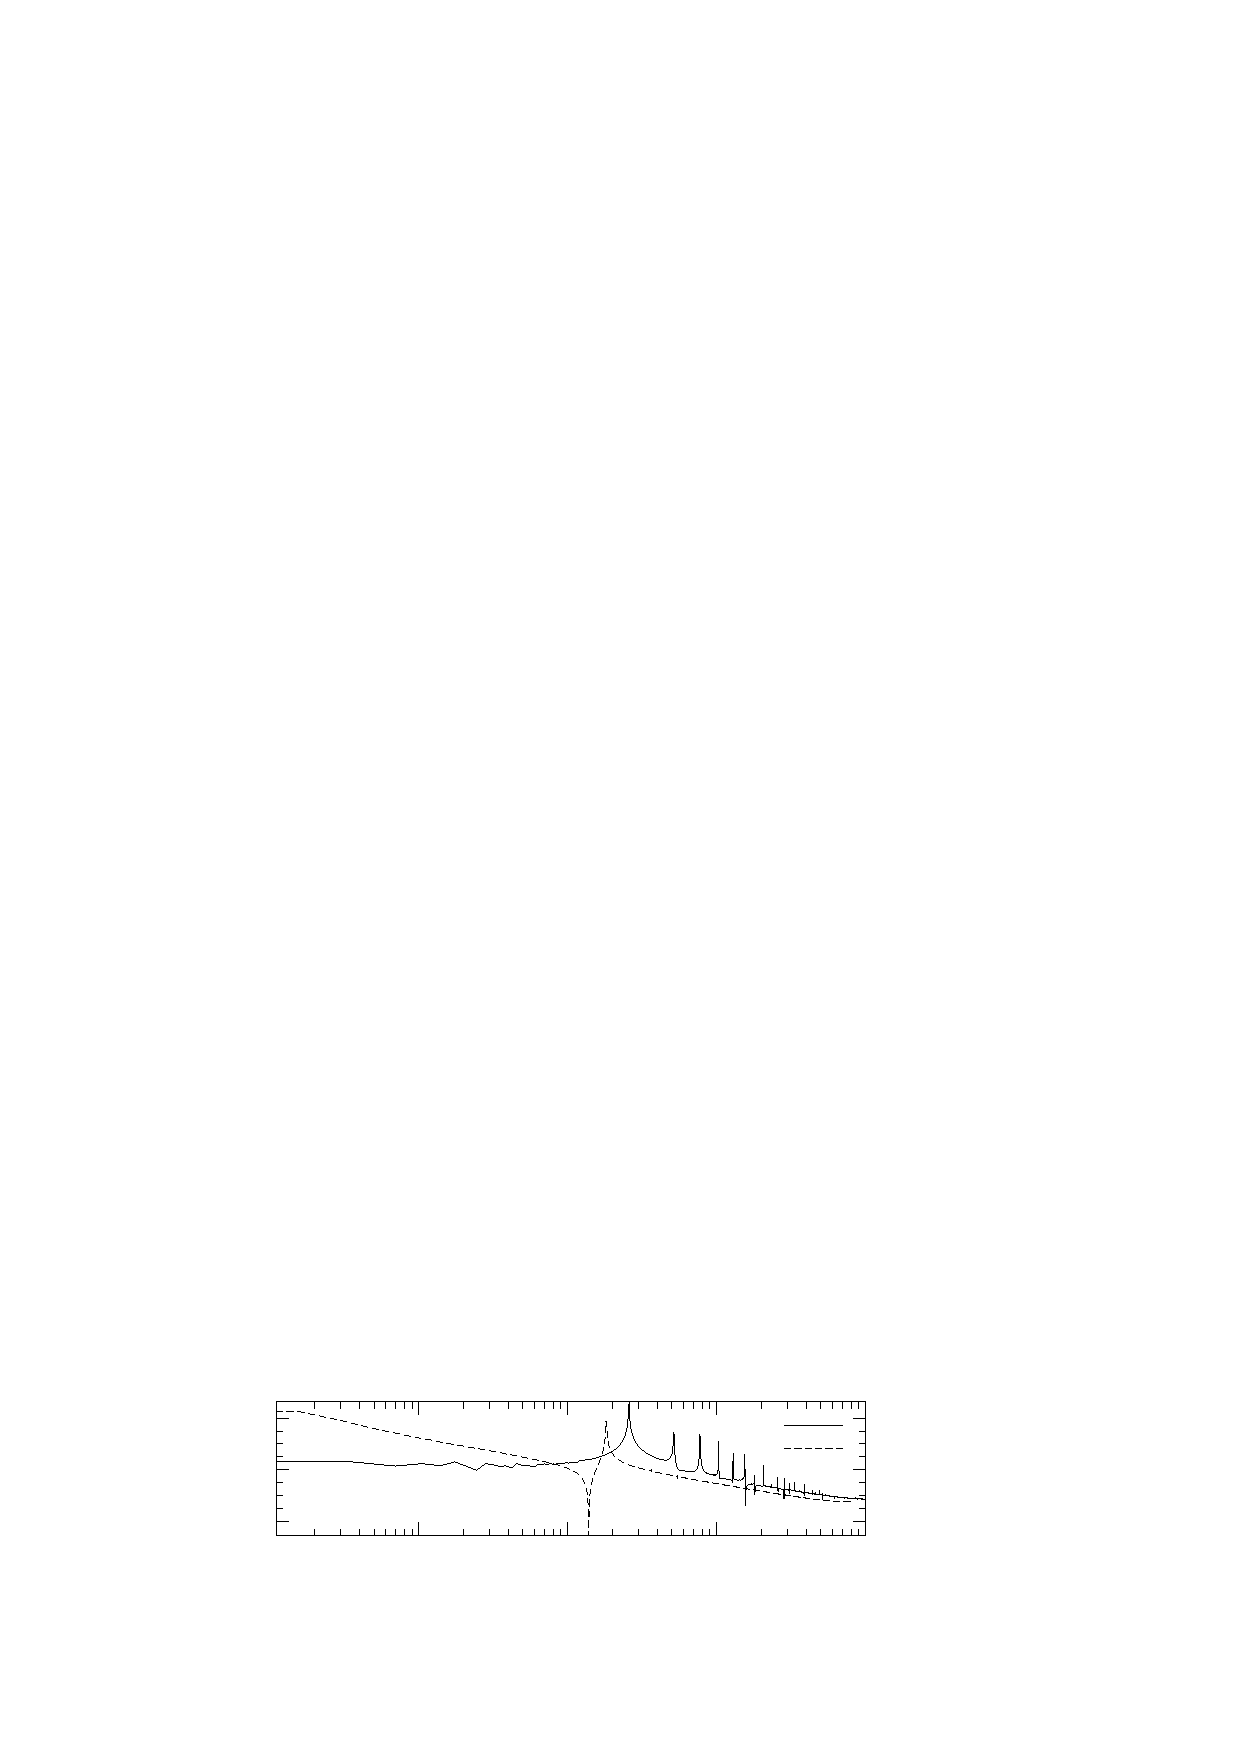
\includegraphics{detalle-frecuencias-rounded-flat-gravity}%
\end{picture}%
\begingroup
\setlength{\unitlength}{0.0200bp}%
\begin{picture}(18000,5400)(0,0)%
\put(2750,1989){\makebox(0,0)[r]{\strut{} 1e-12}}%
\put(2750,3223){\makebox(0,0)[r]{\strut{} 1e-08}}%
\put(2750,4458){\makebox(0,0)[r]{\strut{} 1e-04}}%
\put(6452,1100){\makebox(0,0){\strut{} 0.001}}%
\put(10026,1100){\makebox(0,0){\strut{} 0.01}}%
\put(13601,1100){\makebox(0,0){\strut{} 0.1}}%
\put(17175,1100){\makebox(0,0){\strut{} 1}}%
\put(550,3250){\rotatebox{90}{\makebox(0,0){\strut{}PSD}}}%
\put(10100,275){\makebox(0,0){\strut{}$\omega$}}%
\put(14950,4275){\makebox(0,0)[r]{\strut{}redondeada}}%
\put(14950,3725){\makebox(0,0)[r]{\strut{}plana}}%
\put(600,1000){\rotatebox{0}{\makebox(0,0){\strut{}(b)}}}%
\end{picture}%
\endgroup
\endinput

\caption{\label{fig:detalle-flat-rounded-gravity}
 Posici'on vertical de la part'icula para la cavidad
plana y la redondeada ambas en presencia de un campo gravitacional externo.
Ambas oscilan con la frecuencia de la fuente ac'ustica $\omega_p$
para la cavidad plana y $\omega_r $ para la cavidad redondeada.
}
\end{figure}


En las siguientes simulaciones num'ericas, conservamos todos los valores de los par'ametros y agregamos
la presencia de un campo gravitacional externo. En las figuras~\ref{fig:path-3} (a)
y (b)  mostramos la evoluci'on temporal de la posici'on vertical de una part'icula s'olida en presencia 
de un campo gravitacional externo para la cavidad plana y la redondeada, respectivamente. 
La l'inea s'olida indica la posici'on de los nodos de presi'on para ambas cavidades.
Observamos que la part'icula oscila abajo del nodo de presi'on en ambas cavidades, donde la 
suma de la fuerza ac'ustica y gravitacional es cero. Observamos tambi'en que el desplazamiento 
de la posici'on estacionaria respecto al nodo de presi'on  es mayor 
en la cavidad plana que en la redondeada. De la figura~\ref{fig:detalle-flat-rounded-gravity} observamos  el mismo  
comportamiento para el movimiento vertical de la part'icula que cuando no existe un campo gravitacional externo 
(ver figura~\ref{fig:detalle-flat-rounded} ). 





\begin{figure} 
%\put(15400,4350){\makebox(0,0)[r]{\strut{}(b)}}%
%GNUPLOT: LaTeX picture with Postscript
\begin{picture}(0,0)%
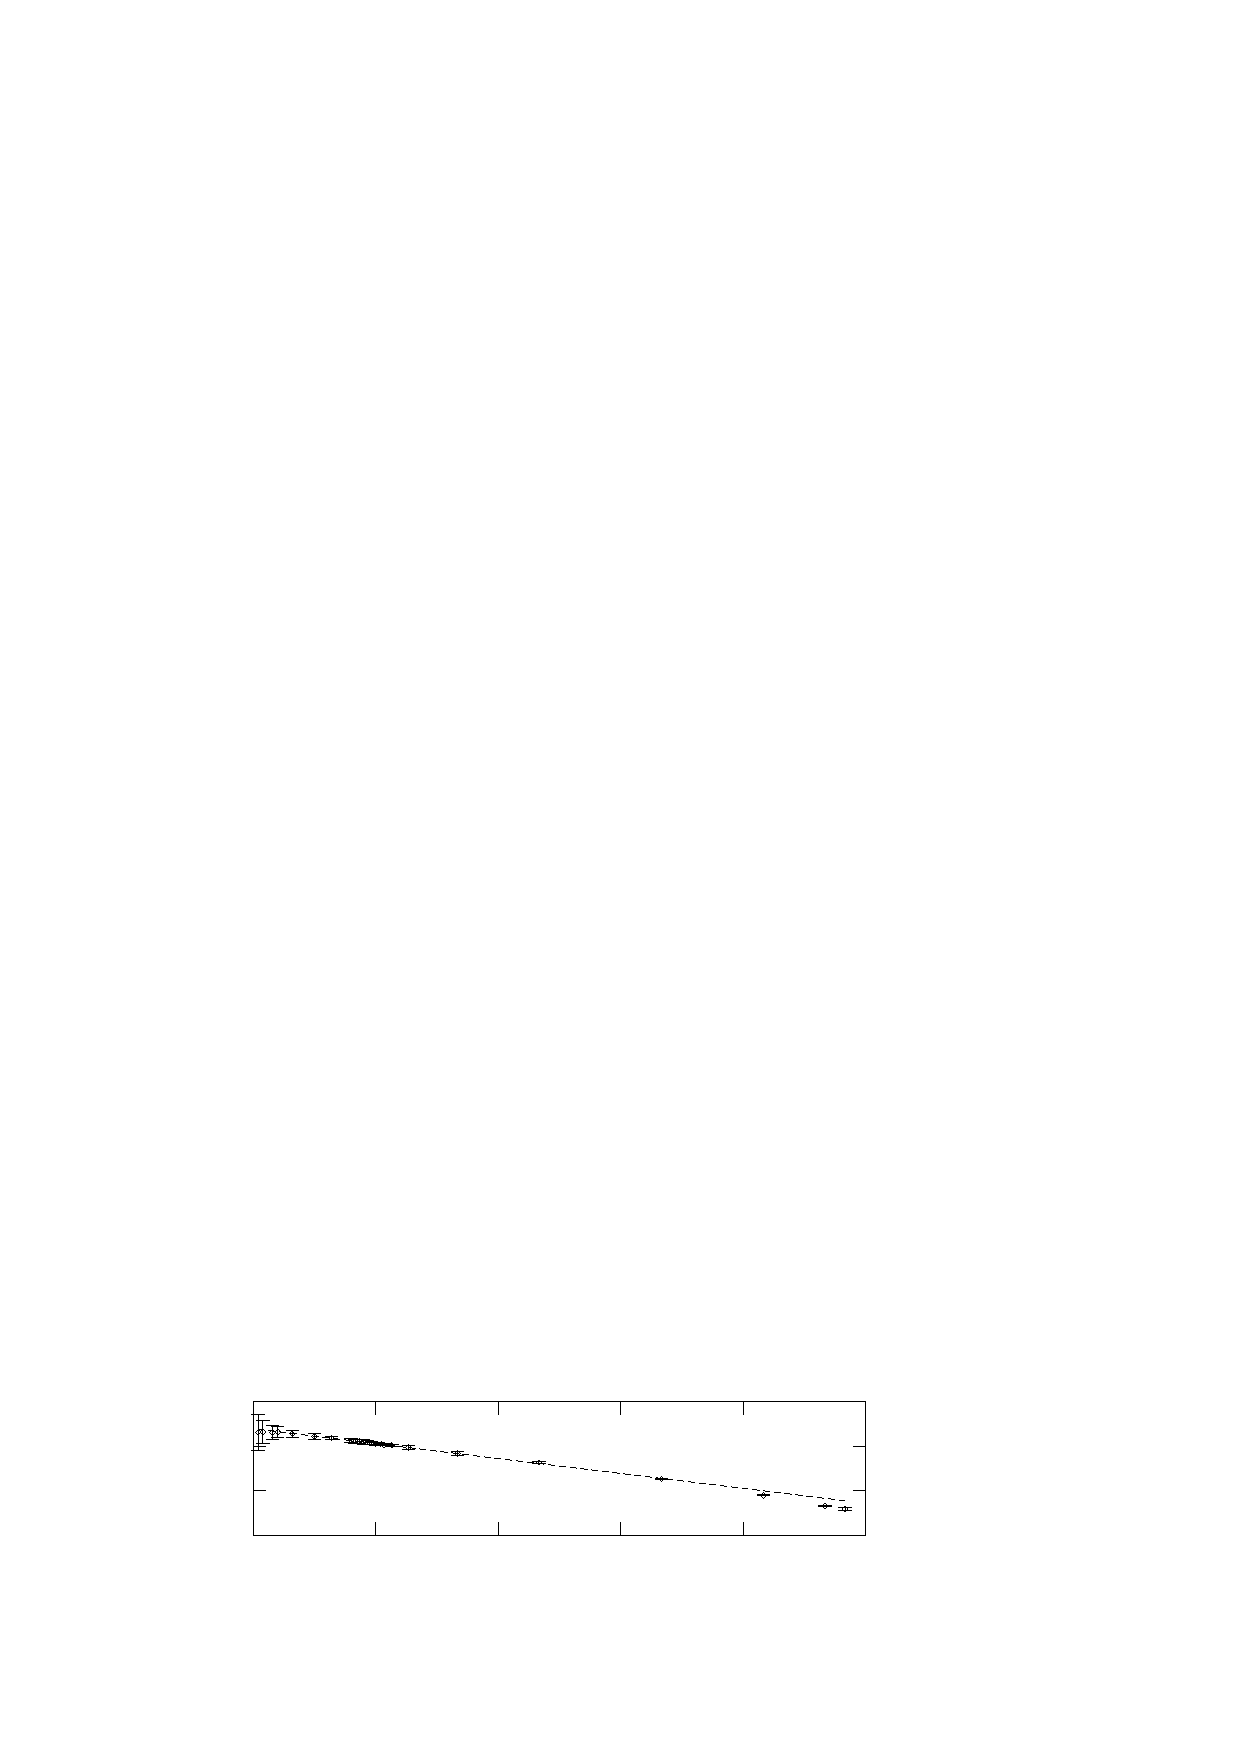
\includegraphics{barrido-rho-flat-ajuste}%
\end{picture}%
\begingroup
\setlength{\unitlength}{0.0200bp}%
\begin{picture}(18000,5400)(0,0)%
\put(2200,1650){\makebox(0,0)[r]{\strut{}1.00}}%
\put(2200,2717){\makebox(0,0)[r]{\strut{}1.25}}%
\put(2200,3783){\makebox(0,0)[r]{\strut{}1.50}}%
\put(2200,4850){\makebox(0,0)[r]{\strut{}1.75}}%
\put(2475,1100){\makebox(0,0){\strut{} 0}}%
\put(5415,1100){\makebox(0,0){\strut{} 50}}%
\put(8355,1100){\makebox(0,0){\strut{} 100}}%
\put(11295,1100){\makebox(0,0){\strut{} 150}}%
\put(14235,1100){\makebox(0,0){\strut{} 200}}%
\put(17175,1100){\makebox(0,0){\strut{} 250}}%
\put(550,3250){\rotatebox{90}{\makebox(0,0){\strut{}$y^\ast_{es}$}}}%
\put(9825,275){\makebox(0,0){\strut{}$\rho_p/\rho_f$}}%
\put(600,1000){\rotatebox{0}{\makebox(0,0){\strut{}(a)}}}%
\end{picture}%
\endgroup
\endinput

%GNUPLOT: LaTeX picture with Postscript
\begin{picture}(0,0)%
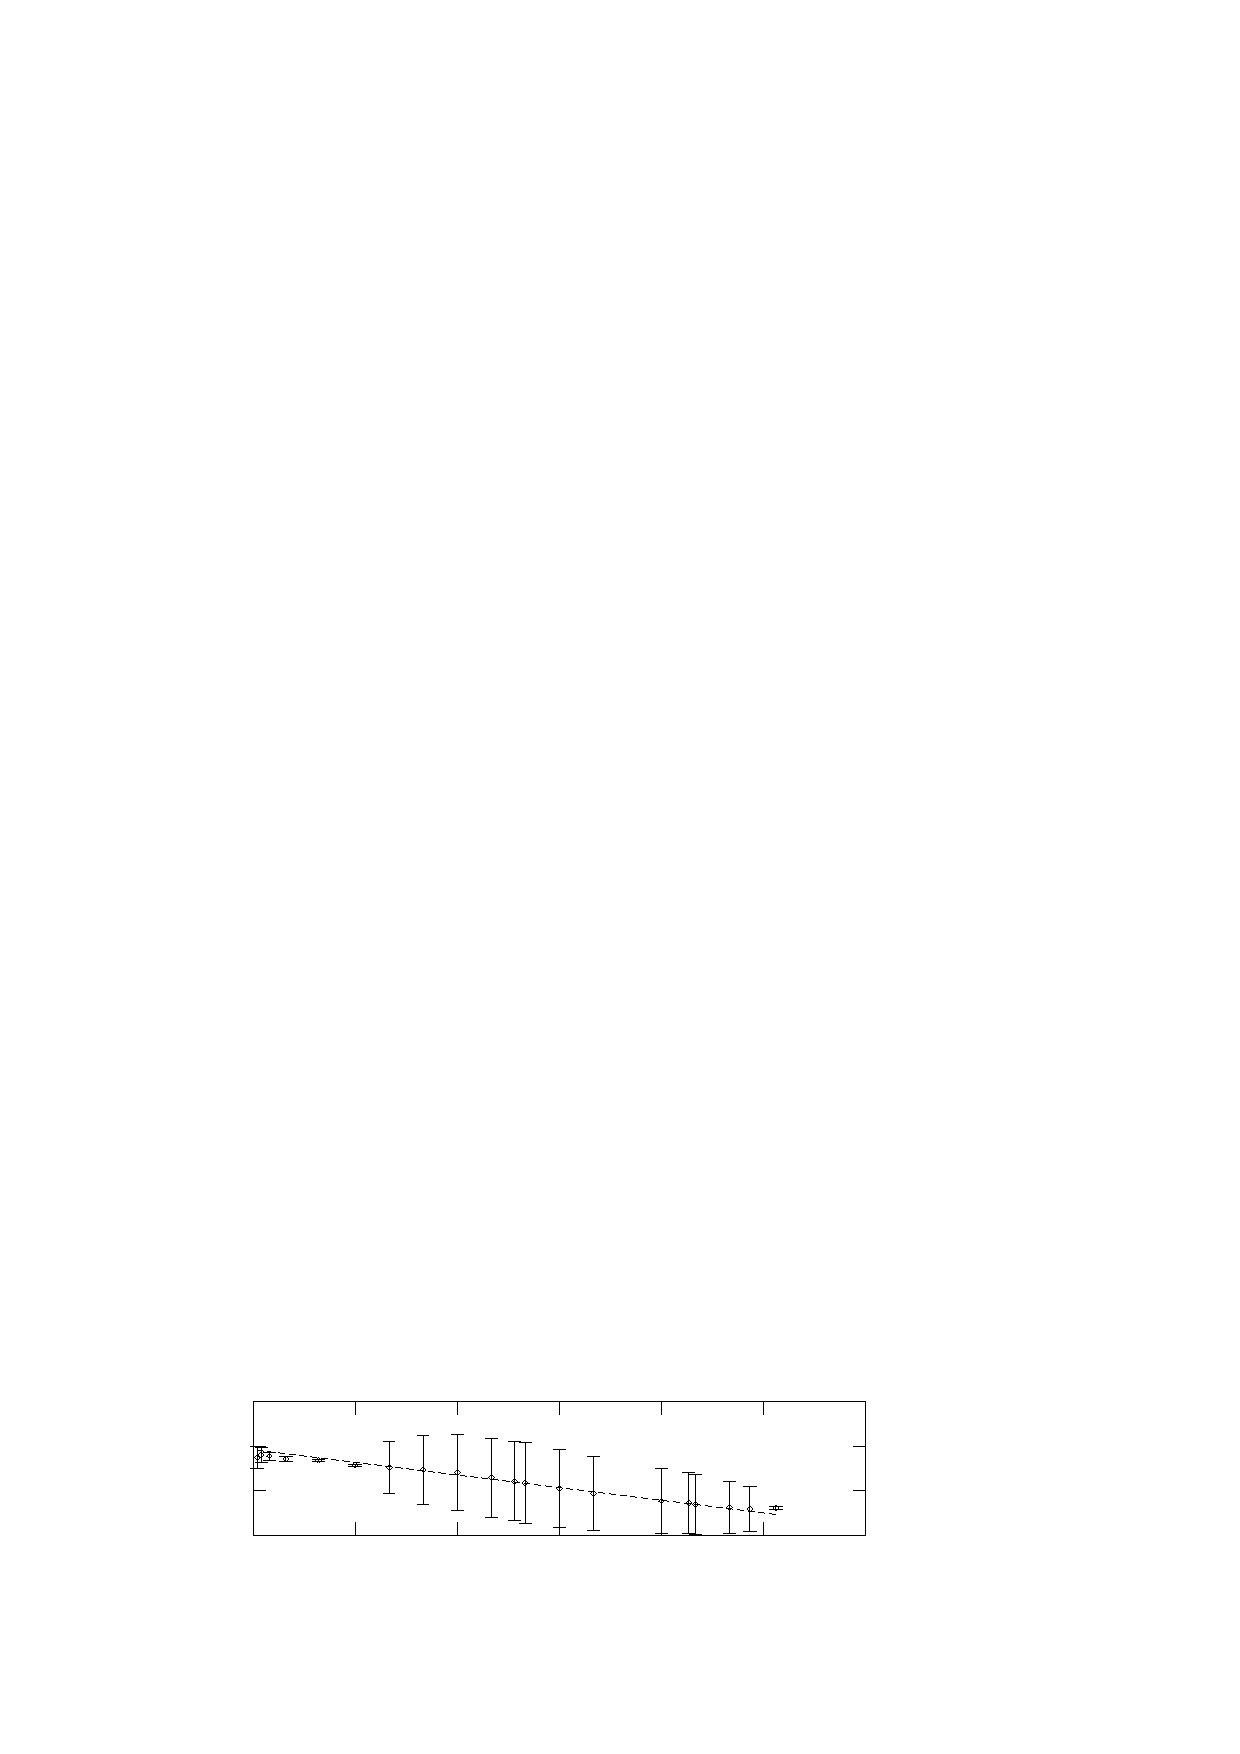
\includegraphics{barrido-rho-rounded-ajuste}%
\end{picture}%
\begingroup
\setlength{\unitlength}{0.0200bp}%
\begin{picture}(18000,5400)(0,0)%
\put(2200,1650){\makebox(0,0)[r]{\strut{}0.80}}%
\put(2200,2717){\makebox(0,0)[r]{\strut{}1.20}}%
\put(2200,3783){\makebox(0,0)[r]{\strut{}1.60}}%
\put(2200,4850){\makebox(0,0)[r]{\strut{}2.00}}%
\put(2475,1100){\makebox(0,0){\strut{} 0}}%
\put(4925,1100){\makebox(0,0){\strut{} 50}}%
\put(7375,1100){\makebox(0,0){\strut{} 100}}%
\put(9825,1100){\makebox(0,0){\strut{} 150}}%
\put(12275,1100){\makebox(0,0){\strut{} 200}}%
\put(14725,1100){\makebox(0,0){\strut{} 250}}%
\put(17175,1100){\makebox(0,0){\strut{} 300}}%
\put(550,3250){\rotatebox{90}{\makebox(0,0){\strut{}$y_{es}^\ast$}}}%
\put(9825,275){\makebox(0,0){\strut{}$\rho_p/\rho_f$}}%
\put(600,1000){\rotatebox{0}{\makebox(0,0){\strut{}(b)}}}%
\end{picture}%
\endgroup
\endinput

%GNUPLOT: LaTeX picture with Postscript
\begin{picture}(0,0)%
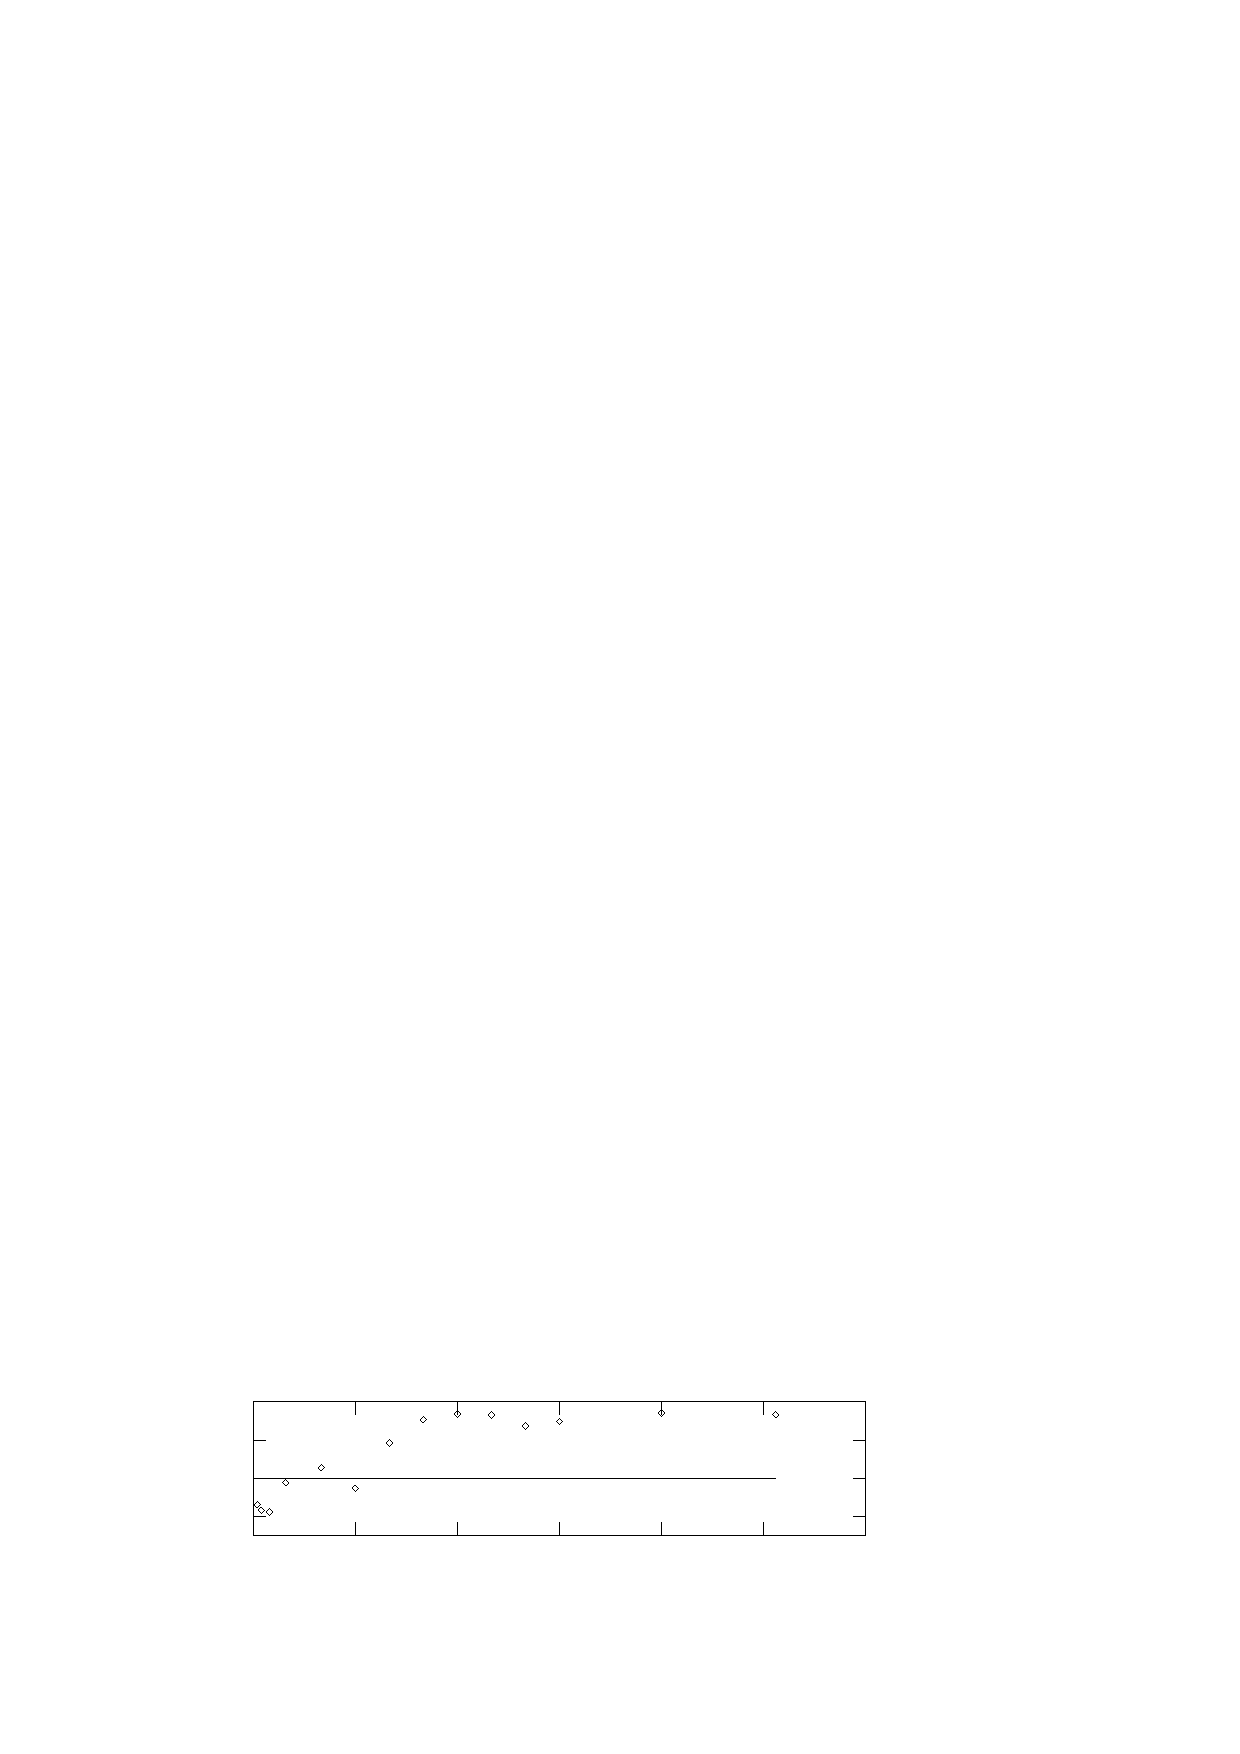
\includegraphics{resonancia-barridorho-rounded}%
\end{picture}%
\begingroup
\setlength{\unitlength}{0.0200bp}%
\begin{picture}(18000,5400)(0,0)%
\put(2200,2107){\makebox(0,0)[r]{\strut{}0.90}}%
\put(2200,3021){\makebox(0,0)[r]{\strut{}1.00}}%
\put(2200,3936){\makebox(0,0)[r]{\strut{}1.10}}%
\put(2200,4850){\makebox(0,0)[r]{\strut{}1.20}}%
\put(2475,1100){\makebox(0,0){\strut{} 0}}%
\put(4925,1100){\makebox(0,0){\strut{} 50}}%
\put(7375,1100){\makebox(0,0){\strut{} 100}}%
\put(9825,1100){\makebox(0,0){\strut{} 150}}%
\put(12275,1100){\makebox(0,0){\strut{} 200}}%
\put(14725,1100){\makebox(0,0){\strut{} 250}}%
\put(17175,1100){\makebox(0,0){\strut{} 300}}%
\put(550,3250){\rotatebox{90}{\makebox(0,0){\strut{}$v_{max}^\ast$}}}%
\put(9825,275){\makebox(0,0){\strut{}$\rho_p/\rho_f$}}%
\put(600,1000){\rotatebox{0}{\makebox(0,0){\strut{}(c)}}}%
\end{picture}%
\endgroup
\endinput

\caption{\label{fig:barrido-rho}
Posici'on y desviaci'on est'andar vertical de la part'icula variando la relaci'on de densidades
y manteniendo la cantidad de movimiento constante en (a) $P_o^\ast=0.01$ para la cavidad plana y 
(b) $P_o\ast=0.0019$ para la redondeada. 
La pendiente de la l'inea ajustada es $-0.001677$ para la cavidad plana y $-0.002274$
para la cavidad redondeada. En (c) mostramos
la velocidad m'axima dentro de la cavidad en presencia de part'icula  para la cavidad redondeada con
$P_o^\ast=0.01$. }
\end{figure}
%
\begin{figure} 
%\put(-180,3250){\rotatebox{90}{\makebox(0,0){\strut{}(a)}}}%
%GNUPLOT: LaTeX picture with Postscript
%\begin{picture}(0,0)%
%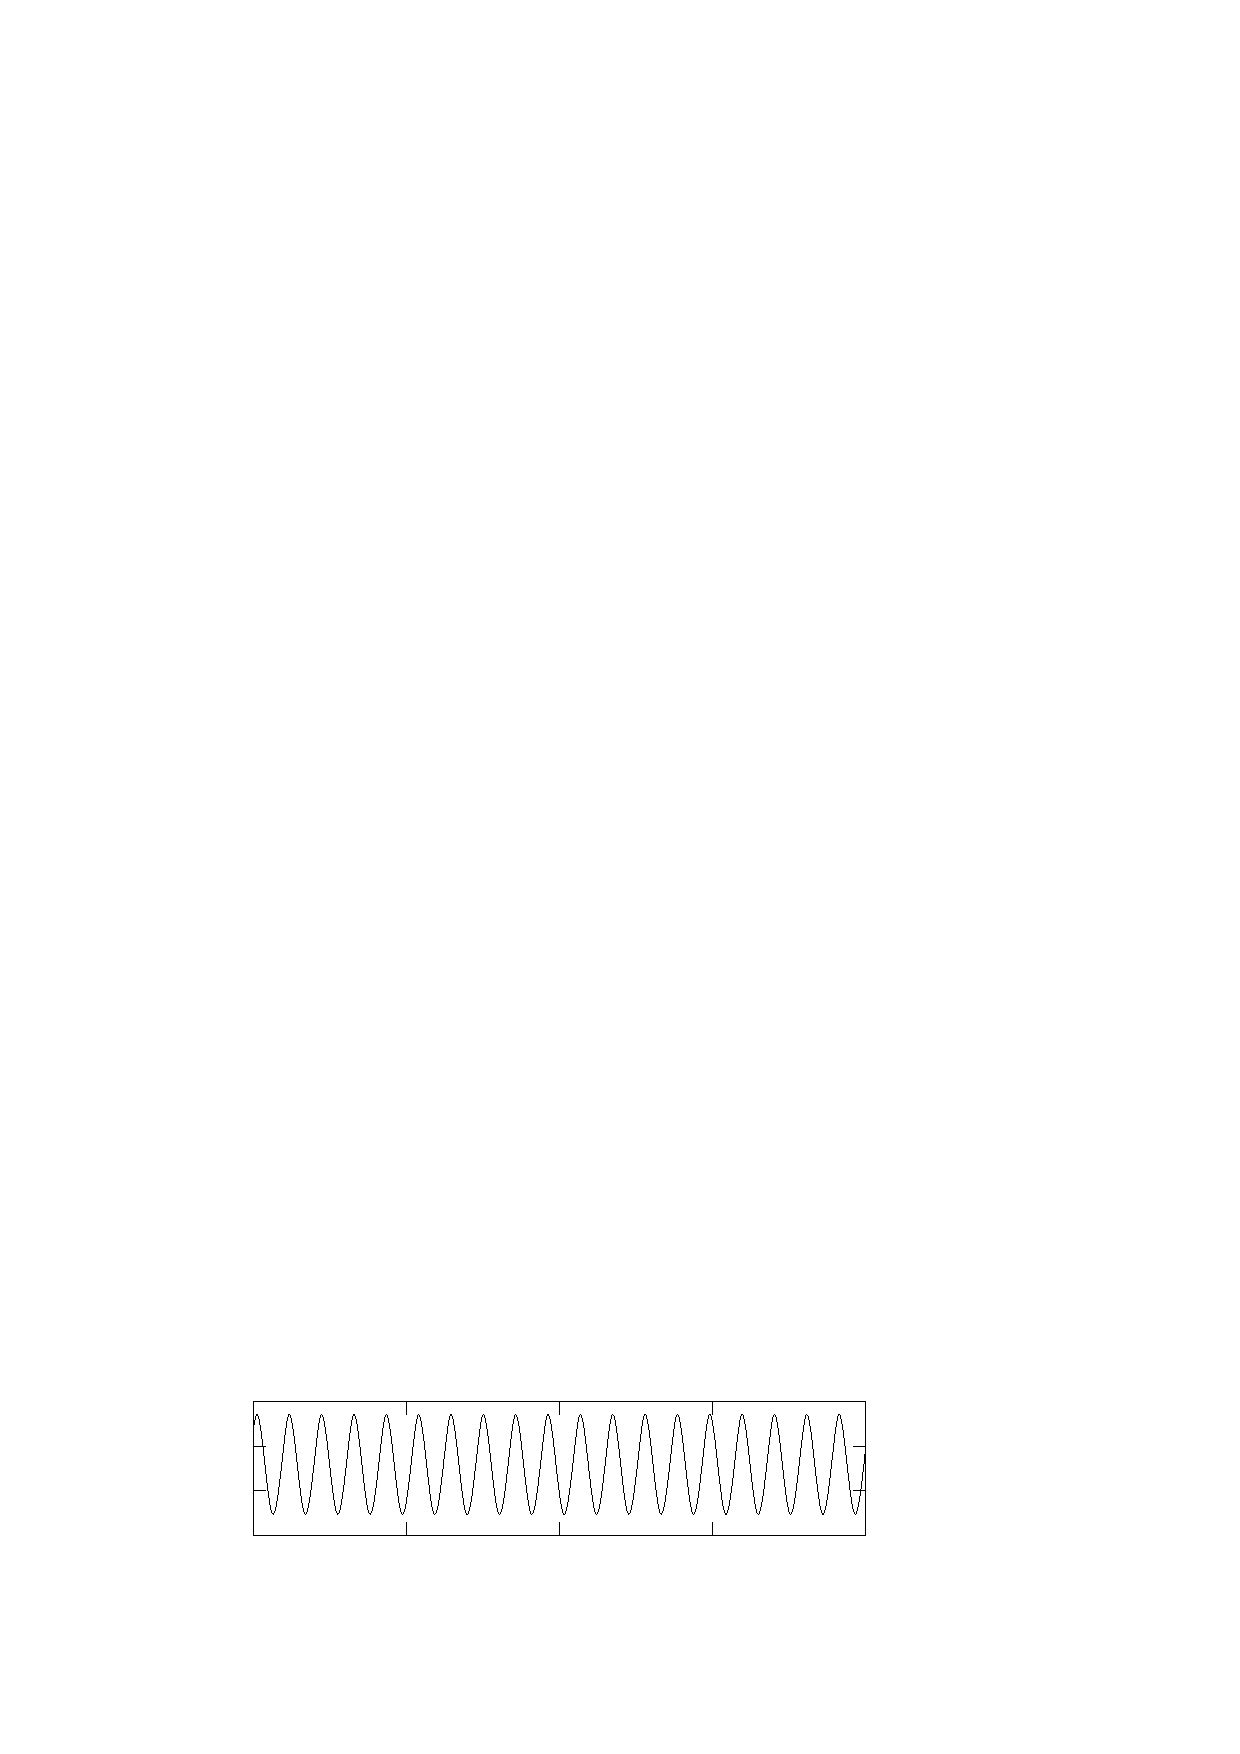
\includegraphics{flat-rhobarrido4_8}%
%\end{picture}%
%\begingroup
%\setlength{\unitlength}{0.0200bp}%
%\begin{picture}(18000,5400)(0,0)%
%\put(2200,1650){\makebox(0,0)[r]{\strut{}1.50}}%
%\put(2200,2717){\makebox(0,0)[r]{\strut{}1.55}}%
%\put(2200,3783){\makebox(0,0)[r]{\strut{}1.60}}%
%\put(2200,4850){\makebox(0,0)[r]{\strut{}1.65}}%
%\put(2475,1100){\makebox(0,0){\strut{} 500}}%
%\put(6150,1100){\makebox(0,0){\strut{} 505}}%
%\put(9825,1100){\makebox(0,0){\strut{} 510}}%
%\put(13500,1100){\makebox(0,0){\strut{} 515}}%
%\put(17175,1100){\makebox(0,0){\strut{} 520}}%
%\put(550,3250){\rotatebox{90}{\makebox(0,0){\strut{}$y^\ast$}}}%
%\put(9825,275){\makebox(0,0){\strut{}$t^\ast$}}%
%\put(600,1000){\rotatebox{0}{\makebox(0,0){\strut{}(a)}}}%
%\end{picture}%
%\endgroup
%\endinput

%GNUPLOT: LaTeX picture with Postscript
%\begin{picture}(0,0)%
%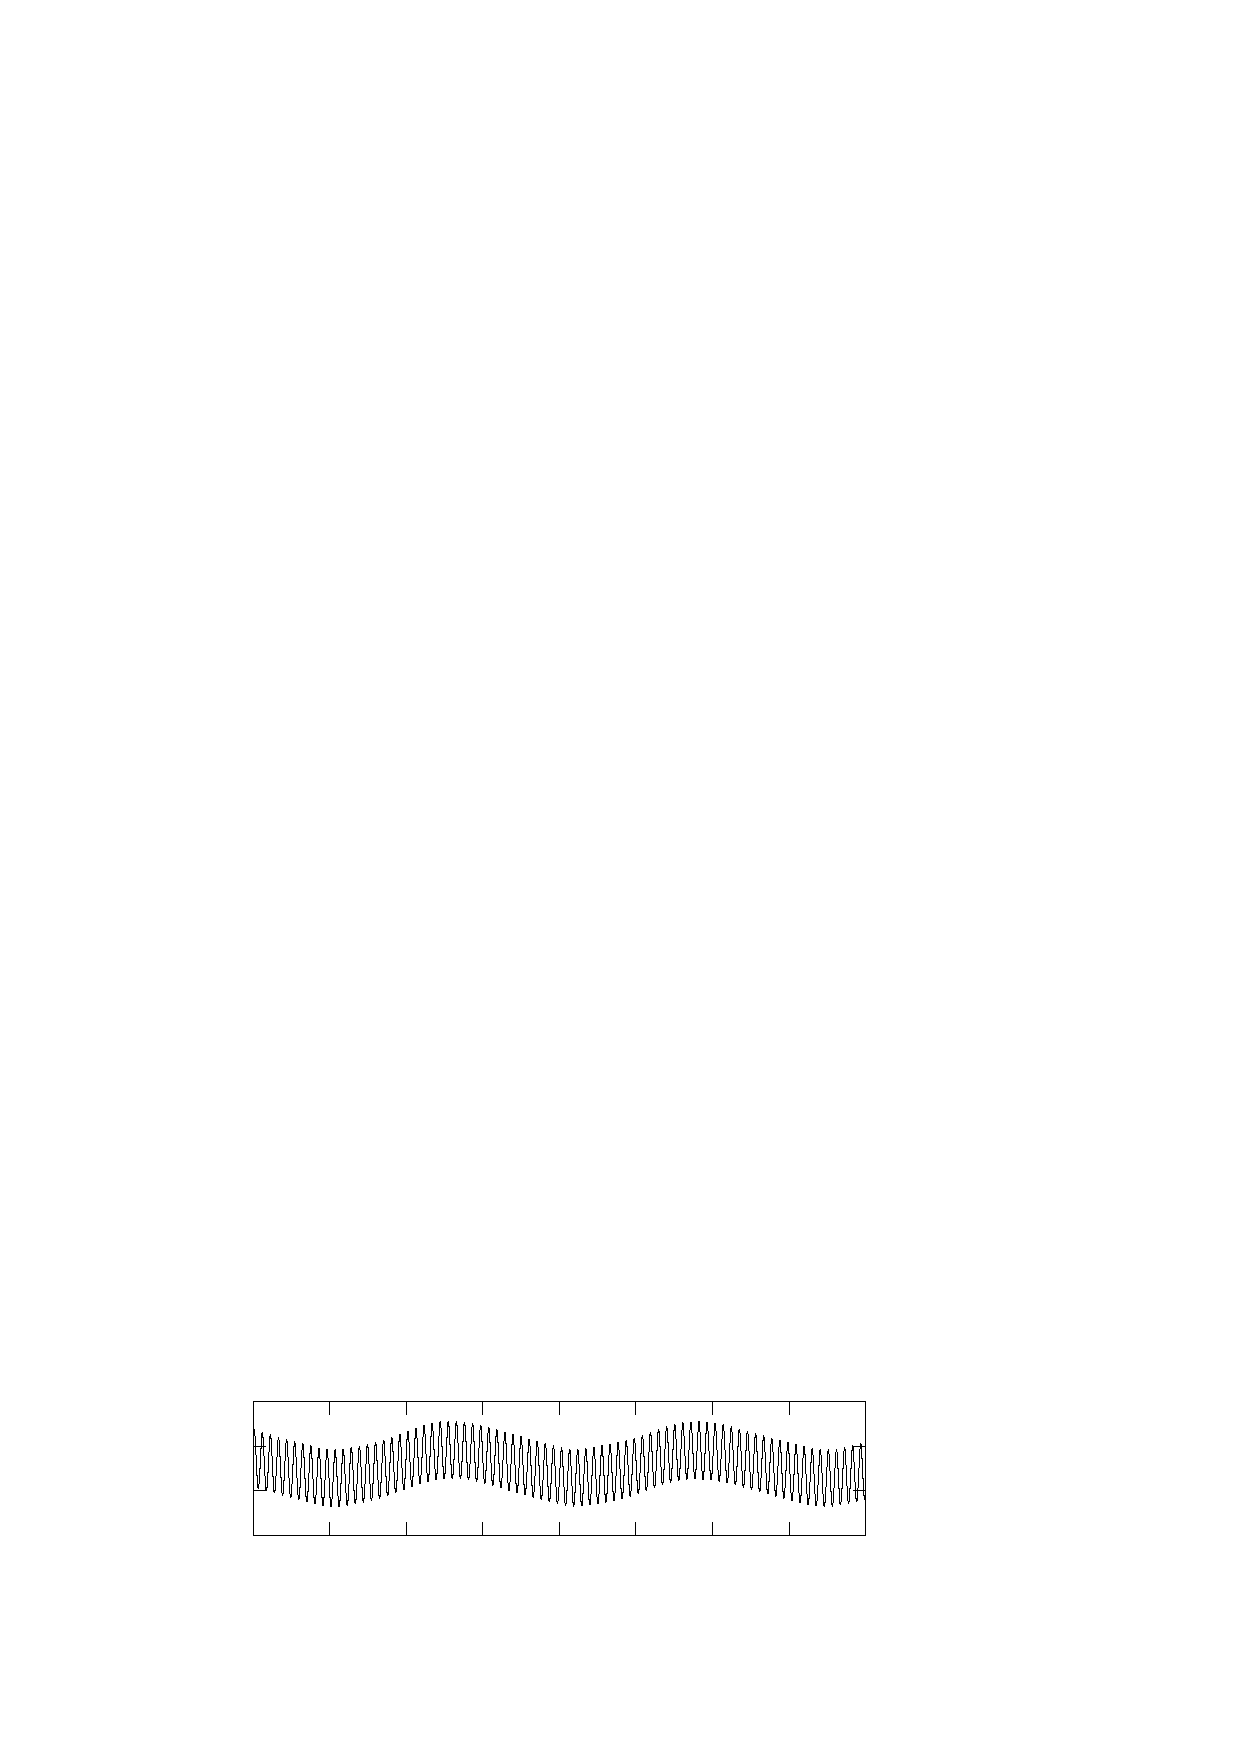
\includegraphics{flat-rhobarrido24}%
%\end{picture}%
%\begingroup
%\setlength{\unitlength}{0.0200bp}%
%\begin{picture}(18000,5400)(0,0)%
%\put(2200,1650){\makebox(0,0)[r]{\strut{}1.50}}%
%\put(2200,2717){\makebox(0,0)[r]{\strut{}1.52}}%
%\put(2200,3783){\makebox(0,0)[r]{\strut{}1.54}}%
%\put(2200,4850){\makebox(0,0)[r]{\strut{}1.56}}%
%\put(2475,1100){\makebox(0,0){\strut{} 500}}%
%\put(4313,1100){\makebox(0,0){\strut{} 510}}%
%\put(6150,1100){\makebox(0,0){\strut{} 520}}%
%\put(7988,1100){\makebox(0,0){\strut{} 530}}%
%\put(9825,1100){\makebox(0,0){\strut{} 540}}%
%\put(11663,1100){\makebox(0,0){\strut{} 550}}%
%\put(13500,1100){\makebox(0,0){\strut{} 560}}%
%\put(15338,1100){\makebox(0,0){\strut{} 570}}%
%\put(17175,1100){\makebox(0,0){\strut{} 580}}%
%\put(550,3250){\rotatebox{90}{\makebox(0,0){\strut{}$y^\ast$}}}%
%\put(9825,275){\makebox(0,0){\strut{}$t^\ast$}}%
%\put(600,1000){\rotatebox{0}{\makebox(0,0){\strut{}(b)}}}%
%\end{picture}%
%\endgroup
%\endinput

%GNUPLOT: LaTeX picture with Postscript
%\begin{picture}(0,0)%
%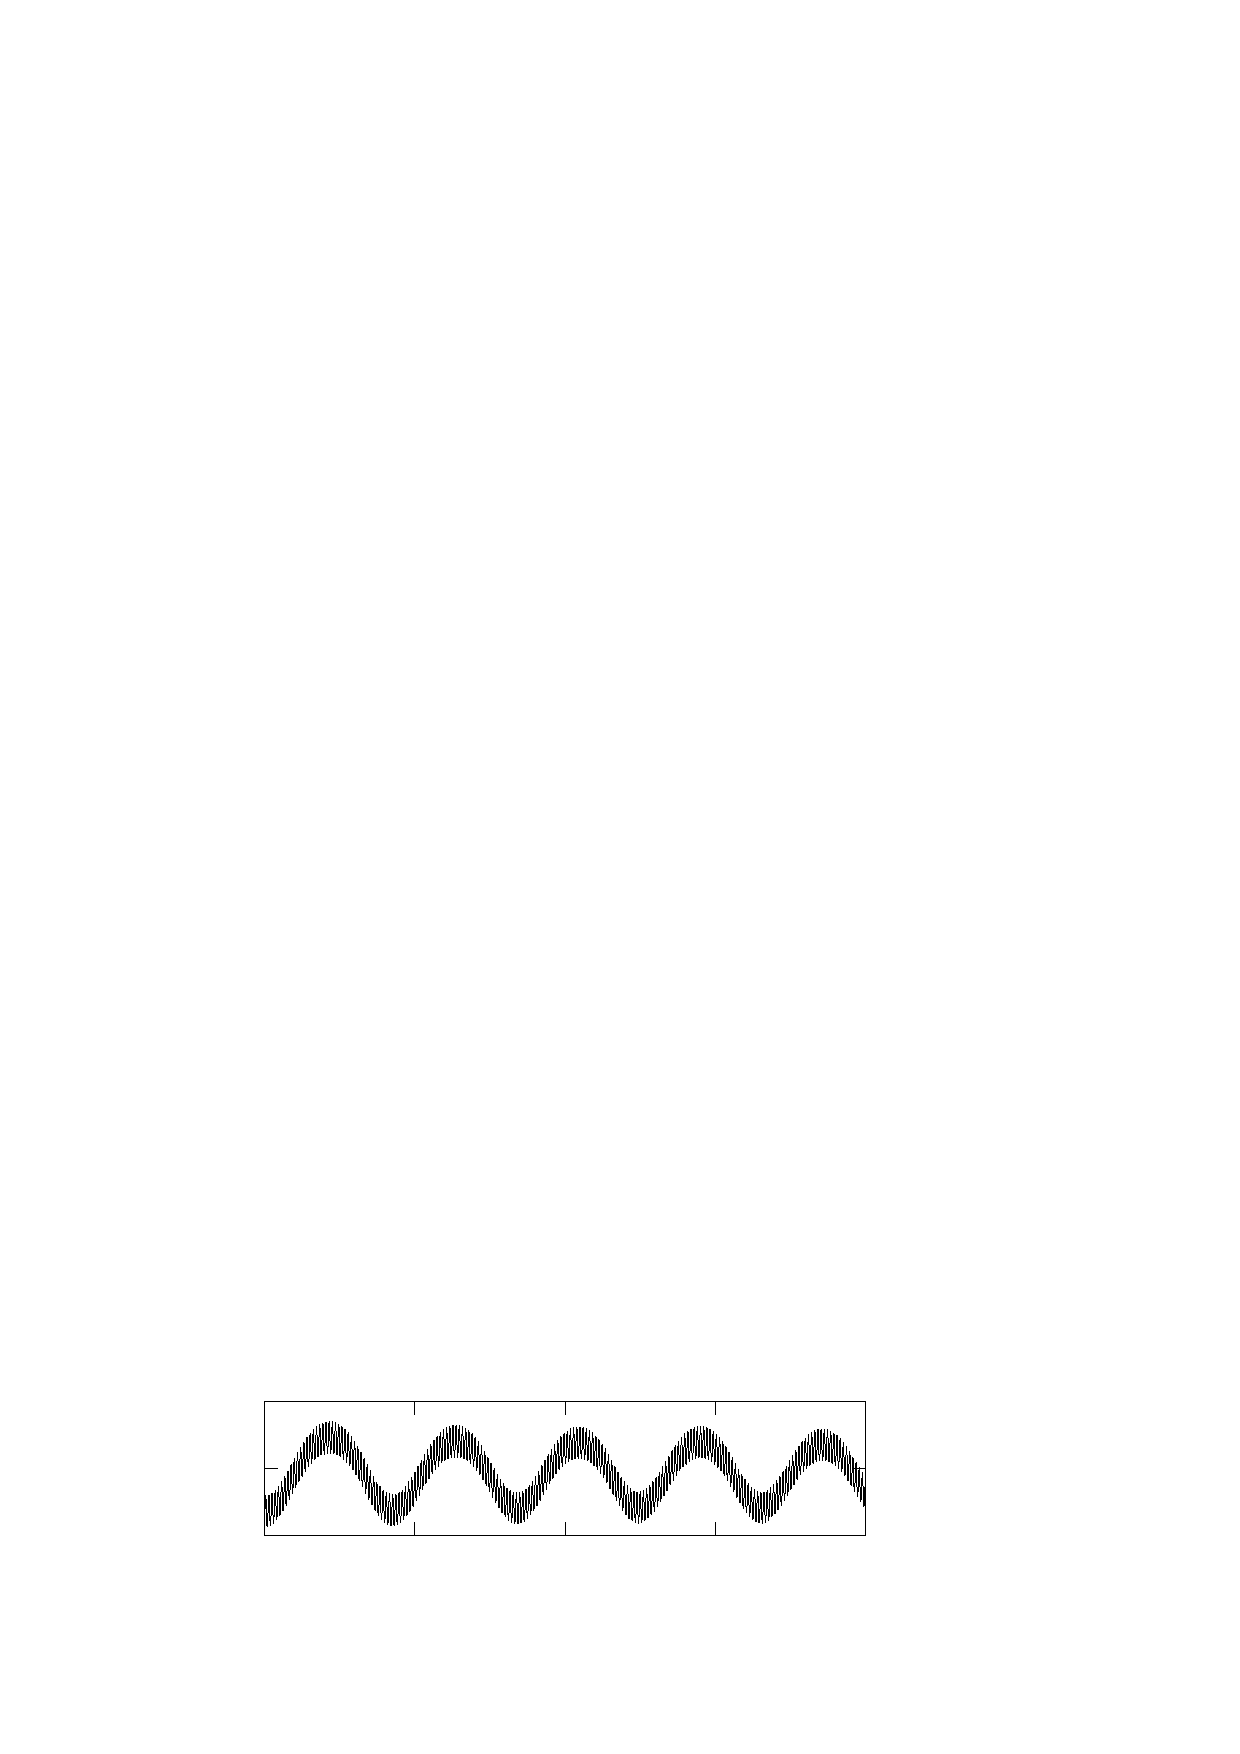
\includegraphics{flat-rhobarrido140}%
%\end{picture}%
%\begingroup
%\setlength{\unitlength}{0.0200bp}%
%\begin{picture}(18000,5400)(0,0)%
%\put(2475,1650){\makebox(0,0)[r]{\strut{}1.156}}%
%\put(2475,3250){\makebox(0,0)[r]{\strut{}1.165}}%
%\put(2475,4850){\makebox(0,0)[r]{\strut{}1.173}}%
%\put(2750,1100){\makebox(0,0){\strut{} 2950}}%
%\put(6356,1100){\makebox(0,0){\strut{} 3000}}%
%\put(9963,1100){\makebox(0,0){\strut{} 3050}}%
%\put(13569,1100){\makebox(0,0){\strut{} 3100}}%
%\put(17175,1100){\makebox(0,0){\strut{} 3150}}%
%\put(550,3250){\rotatebox{90}{\makebox(0,0){\strut{}$y^\ast$}}}%
%\put(9962,275){\makebox(0,0){\strut{}$t^\ast$}}%
%\put(600,1000){\rotatebox{0}{\makebox(0,0){\strut{}(c)}}}%
%\end{picture}%
%\endgroup
%\endinput

\caption{\label{fig:paths-flat}
Posici'on vertical de la part'icula s'olida en funci'on  del tiempo en la cavidad plana para
(a) $ \rho_p/\rho_f = 8$, (b) $\rho_p/\rho_f = 40$ y (c) $\rho_p/\rho_f = 233.3$. En (b)
y (c) observamos una segunda frecuencia de oscilaci'on.
}
\end{figure}
%
\begin{figure} 
%\put(600,2550){\rotatebox{90}{\makebox(0,0){\strut{}(a)}}}%
%GNUPLOT: LaTeX picture with Postscript
%\begin{picture}(0,0)%
%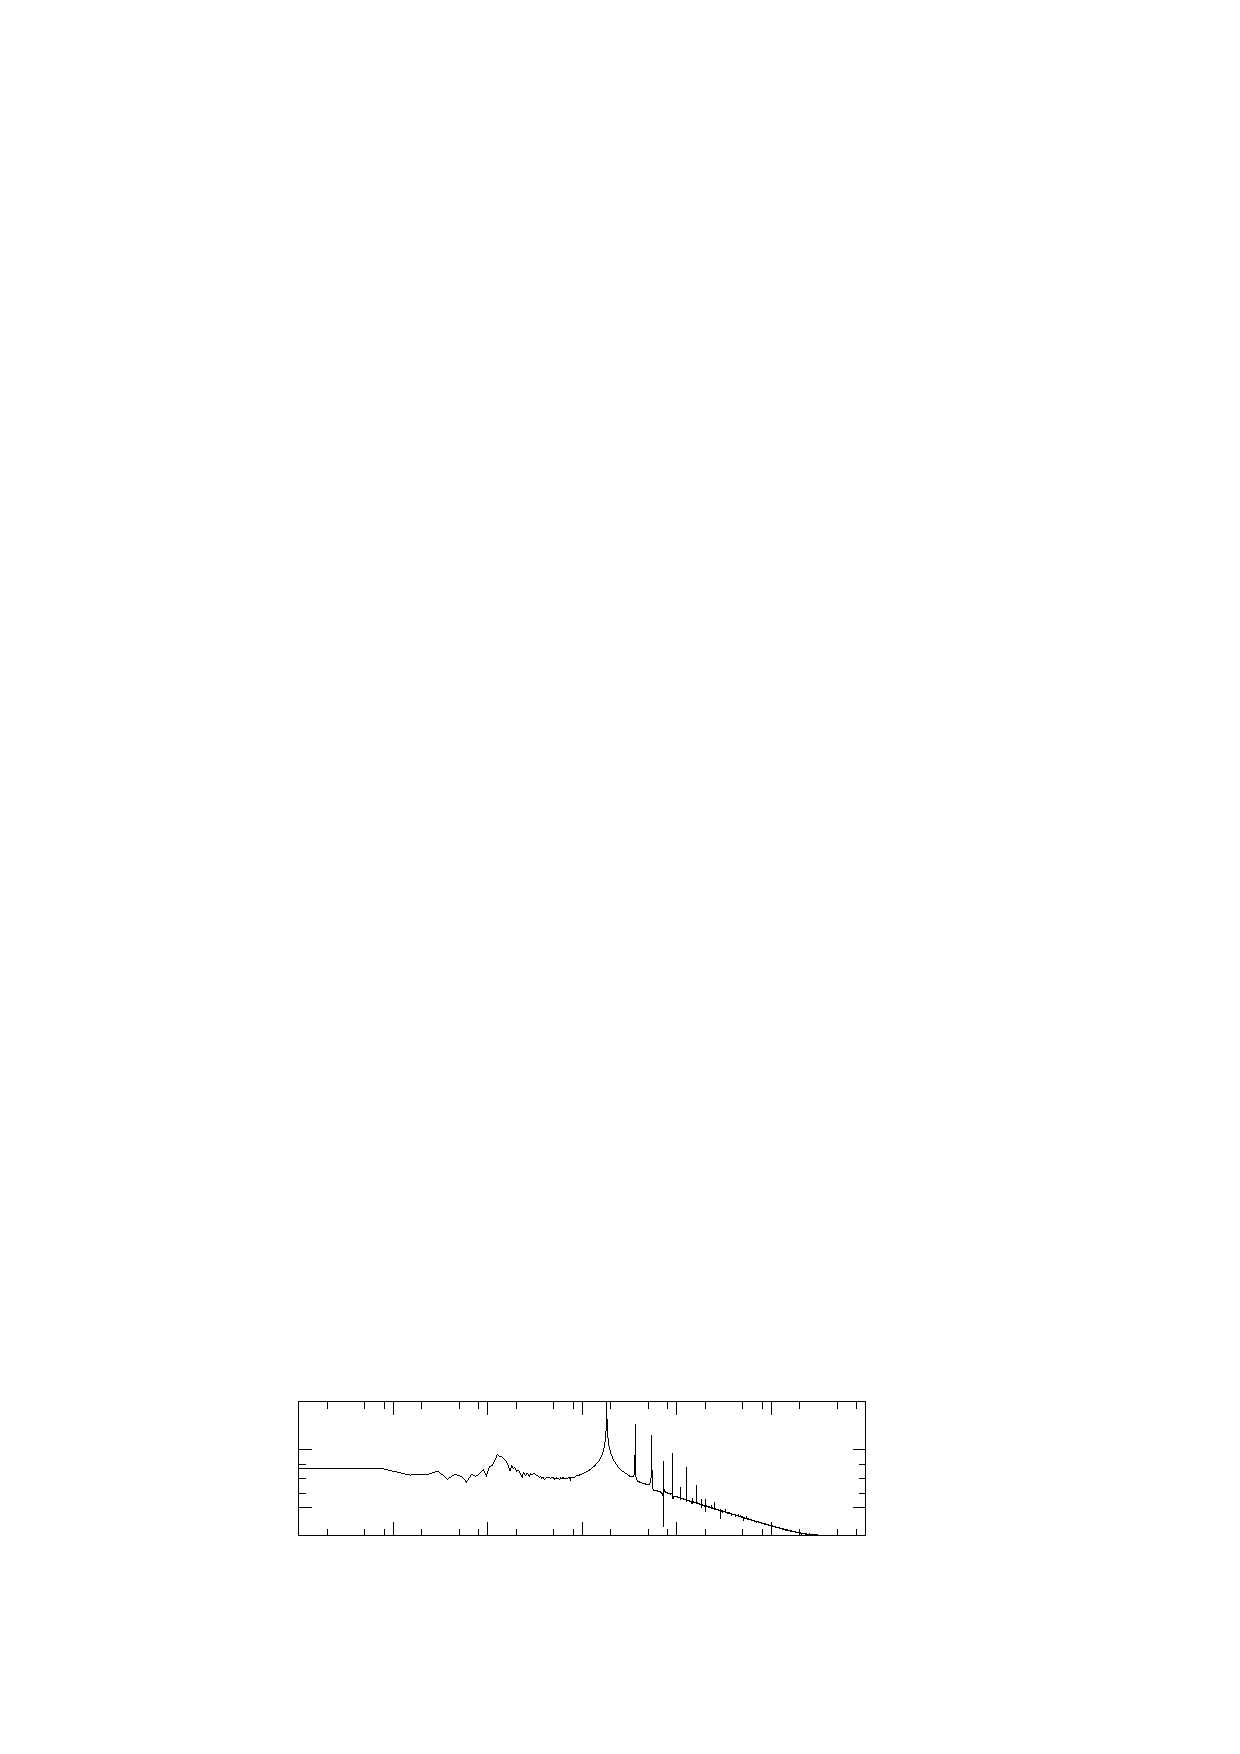
\includegraphics{flat-rhobarrido4_8-spectrum}%
%\end{picture}%
%\begingroup
%\setlength{\unitlength}{0.0200bp}%
%\begin{picture}(18000,5400)(0,0)%
%\put(3300,2307){\makebox(0,0)[r]{\strut{}1.00e-12}}%
%\put(3300,3707){\makebox(0,0)[r]{\strut{}1.00e-08}}%
%\put(3575,1100){\makebox(0,0){\strut{} 1e-05}}%
%\put(5842,1100){\makebox(0,0){\strut{} 1e-04}}%
%\put(8108,1100){\makebox(0,0){\strut{} 0.001}}%
%\put(10375,1100){\makebox(0,0){\strut{} 0.01}}%
%\put(12642,1100){\makebox(0,0){\strut{} 0.1}}%
%\put(14908,1100){\makebox(0,0){\strut{} 1}}%
%\put(17175,1100){\makebox(0,0){\strut{} 10}}%
%\put(550,3250){\rotatebox{90}{\makebox(0,0){\strut{}$PSD$}}}%
%\put(10375,275){\makebox(0,0){\strut{}$\omega$}}%
%\put(600,1000){\rotatebox{0}{\makebox(0,0){\strut{}(a)}}}%
%\end{picture}%
%\endgroup
%\endinput

%GNUPLOT: LaTeX picture with Postscript
%\begin{picture}(0,0)%
%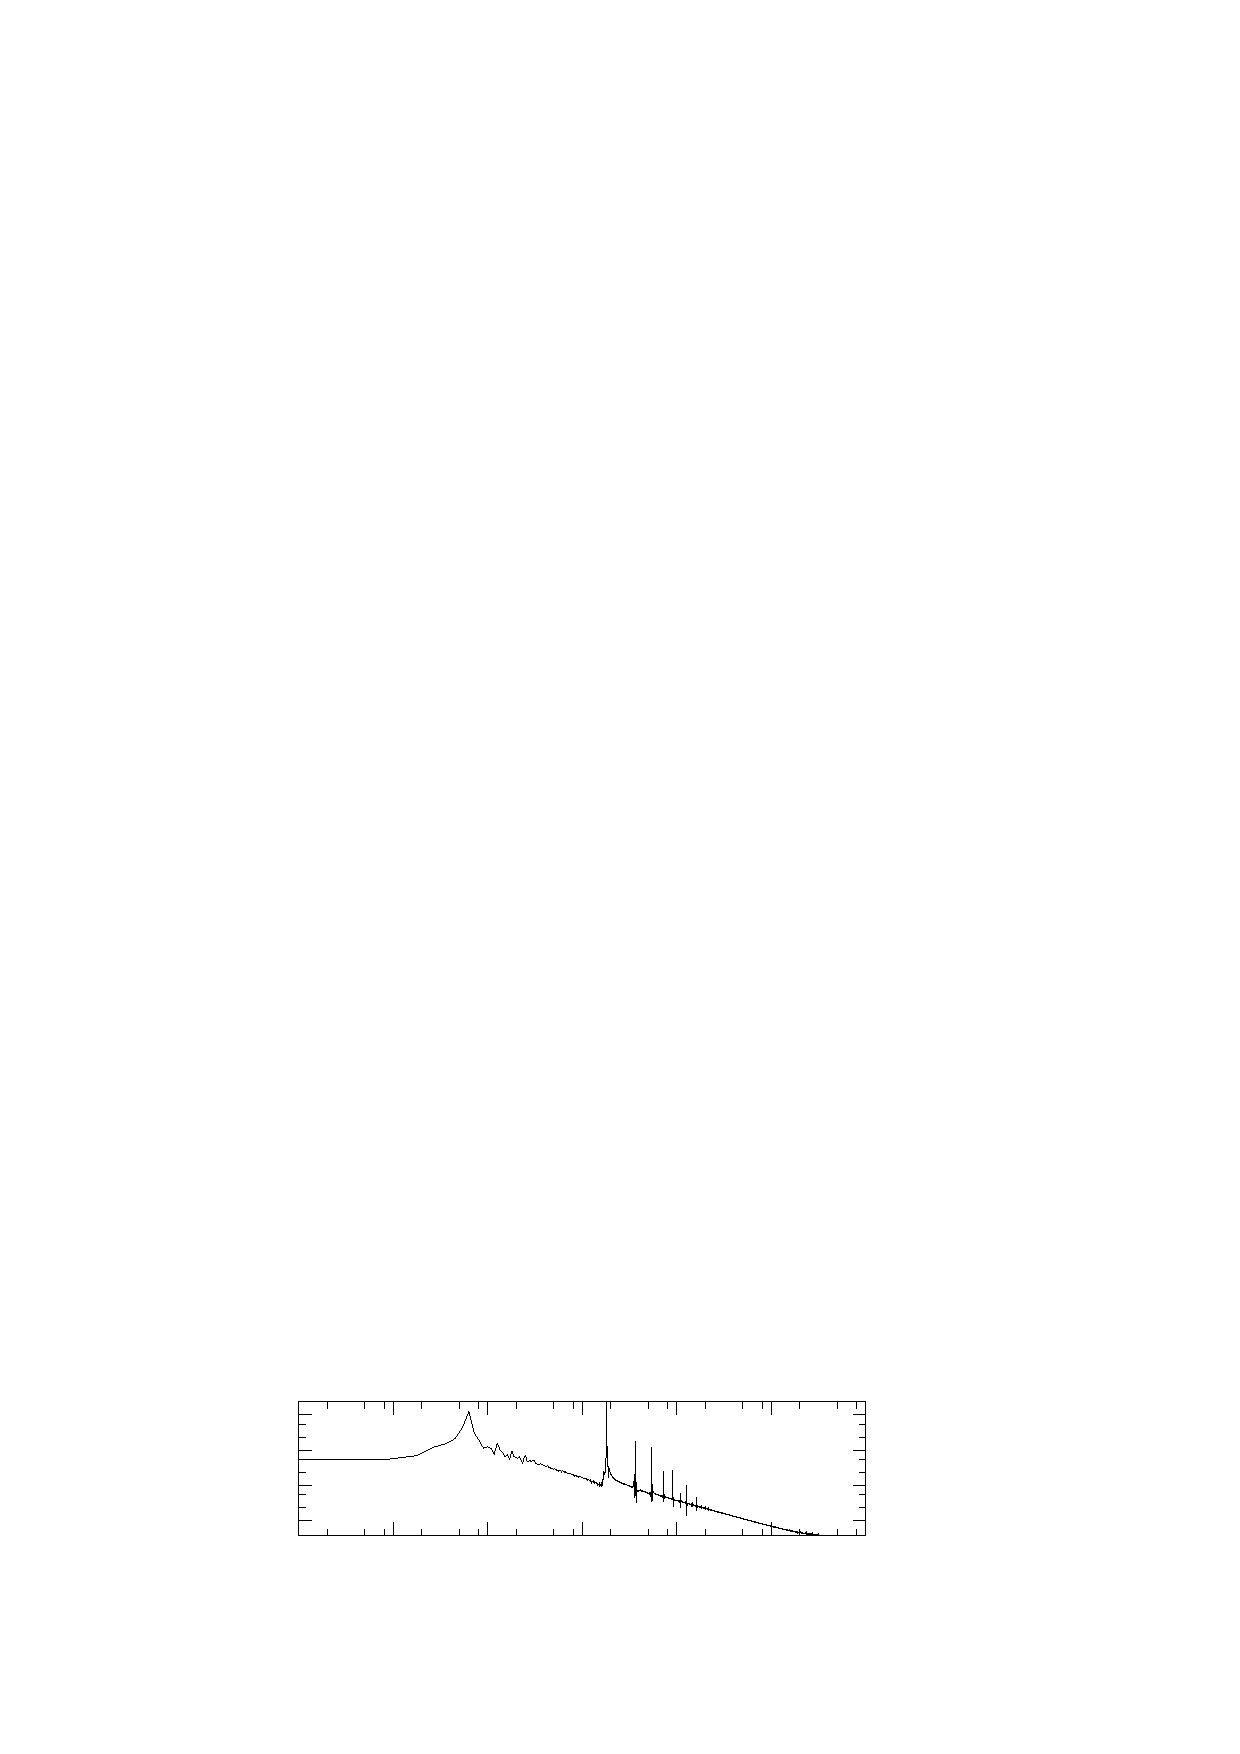
\includegraphics{flat-rhobarrido24-spectrum}%
%\end{picture}%
%\begingroup
%\setlength{\unitlength}{0.0200bp}%
%\begin{picture}(18000,5400)(0,0)%
%\put(3300,2000){\makebox(0,0)[r]{\strut{}3.20e-14}}%
%\put(3300,2846){\makebox(0,0)[r]{\strut{}1.60e-11}}%
%\put(3300,3693){\makebox(0,0)[r]{\strut{}8.00e-09}}%
%\put(3300,4539){\makebox(0,0)[r]{\strut{}4.00e-06}}%
%\put(3575,1100){\makebox(0,0){\strut{} 1e-05}}%
%\put(5842,1100){\makebox(0,0){\strut{} 1e-04}}%
%\put(8108,1100){\makebox(0,0){\strut{} 0.001}}%
%\put(10375,1100){\makebox(0,0){\strut{} 0.01}}%
%\put(12642,1100){\makebox(0,0){\strut{} 0.1}}%
%\put(14908,1100){\makebox(0,0){\strut{} 1}}%
%\put(17175,1100){\makebox(0,0){\strut{} 10}}%
%\put(550,3250){\rotatebox{90}{\makebox(0,0){\strut{}$PSD$}}}%
%\put(10375,275){\makebox(0,0){\strut{}$\omega$}}%
%\put(600,1000){\rotatebox{0}{\makebox(0,0){\strut{}(b)}}}%
%\end{picture}%
%\endgroup
%\endinput

%GNUPLOT: LaTeX picture with Postscript
%\begin{picture}(0,0)%
%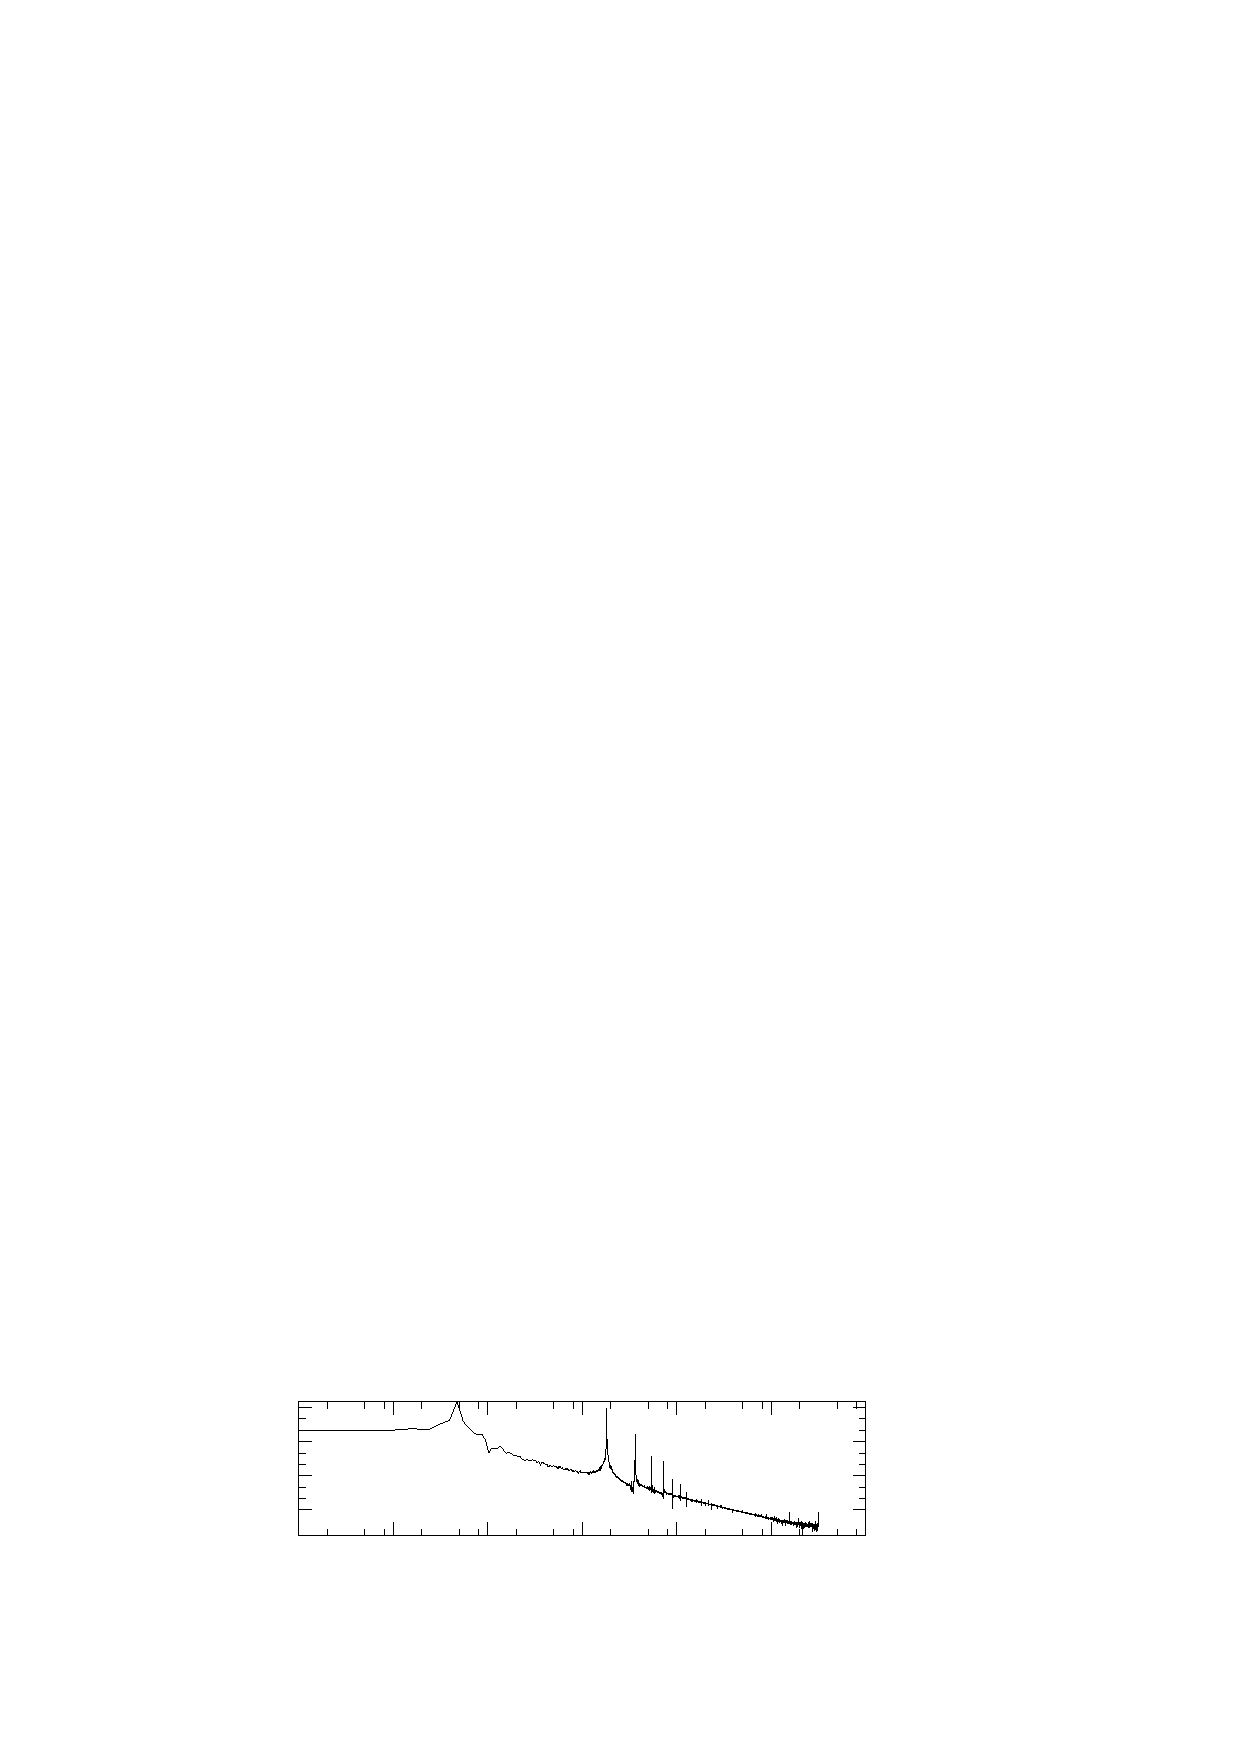
\includegraphics{flat-rhobarrido140-spectrum}%
%\end{picture}%
%\begingroup
%\setlength{\unitlength}{0.0200bp}%
%\begin{picture}(18000,5400)(0,0)%
%\put(3300,2259){\makebox(0,0)[r]{\strut{}1.00e-15}}%
%\put(3300,3077){\makebox(0,0)[r]{\strut{}1.00e-12}}%
%\put(3300,3896){\makebox(0,0)[r]{\strut{}1.00e-09}}%
%\put(3300,4714){\makebox(0,0)[r]{\strut{}1.00e-06}}%
%\put(3575,1100){\makebox(0,0){\strut{} 1e-05}}%
%\put(5842,1100){\makebox(0,0){\strut{} 1e-04}}%
%\put(8108,1100){\makebox(0,0){\strut{} 0.001}}%
%\put(10375,1100){\makebox(0,0){\strut{} 0.01}}%
%\put(12642,1100){\makebox(0,0){\strut{} 0.1}}%
%\put(14908,1100){\makebox(0,0){\strut{} 1}}%
%\put(17175,1100){\makebox(0,0){\strut{} 10}}%
%\put(550,3250){\rotatebox{90}{\makebox(0,0){\strut{}$PSD$}}}%
%\put(10375,275){\makebox(0,0){\strut{}$\omega$}}%
%\put(600,1000){\rotatebox{0}{\makebox(0,0){\strut{}(c)}}}%
%\end{picture}%
%\endgroup
%\endinput

\caption{\label{fig:spectrum-flat}
Espectros de potencia del movimiento vertical de la part'icula s'olida sobre el tiempo en la cavidad plana para
(a) $\rho_p/\rho_f = 8$, (b) $\rho_p/\rho_f = 40$ y (c) $\rho_p/\rho_f = 233.3$. 
Los espectros de potencia corresponden a las oscilaciones reportadas en las figuras~\ref{fig:paths-flat} (a), (b) y (c). 
En (b) podemos observar una segunda frecuencia $\omega=0.000632$ y en (c) $\omega=0.000472$.
}
\end{figure}

En el siguiente conjunto de simulaciones num'ericas,   colocamos inicialmente la part'icula
cerca del nodo de presi'on inferior. La cantidad de movimiento agregada por la fuente ac'ustica
la  mantenemos constante mientras variamos la relaci'on de densidades entre la part'icula y el fluido $\rho_p/\rho_f$.
Para la cavidad plana fijamos la cantidad de movimiento 
en $P_o^\ast=0.01$ y para la cavidad redondeada en $P_o^\ast=0.0019$.
El movimiento de la part'icula, como mostramos m'as adelante, puede llegar a ser 
muy complejo, por lo que adem'as de la posici'on estacionaria, medimos la desviaci'on est'andar 
del movimiento de la part'icula en ambos ejes $\sigma_x$ y $\sigma_y$  para ambas cavidades. En este
caso, la desviaci'on est'andar es una medida de la amplitud de las oscilaciones.
En estas simulaciones, colocamos la part'icula  inicialmente en el eje vertical de la cavidad, cerca 
del nodo inferior de presi'on, y descartamos el transiente en el cual 'esta alcanza un estado
estacionario. Observamos que no hay movimiento de la part'icula en la direcci'on horizontal.
En las figuras~\ref{fig:barrido-rho} (a) y (b), presentamos las posiciones estacionarias y 
$\sigma_y$ en funci'on de la relaci'on de densidades entre la part'icula y el fluido para la cavidad
plana y la redondeada, respectivamente. Conforme
la relaci'on de densidades aumenta es m'as dif'icil que el campo ac'ustico pueda mover la part'icula
y  la posici'on estacionaria se desplaza hacia abajo, como 
mostramos en las figuras~\ref{fig:barrido-rho} (a) y (b). De esto concluimos que la fuerza
ac'ustica aumenta al alejarse del nodo de presi'on, pues la part'icula levita donde la fuerza ac'ustica
es igual al peso de la part'icula. El desplazamiento de la posici'on
estacionaria es lineal entre $40< \rho_p/\rho_f < 200$, como observamos
del ajuste en la figura~\ref{fig:barrido-rho} (a), para la cavidad plana.
En la cavidad redondeada, el desplazamiento de la posici'on estacionaria tambi'en es lineal
en una zona, entre $50<\rho_p/\rho_f < 230$, como observamos 
en la figura~\ref{fig:barrido-rho} (b) por el ajuste de la l'inea discontinua.


La frecuencia de resonancia para cada cavidad la calculamos en ausencia de part'icula. Sabemos
que existe un desplazamiento en la frecuencia de resonancia y que es funci'on del tama~no 
y posici'on de la part'icula dentro de la cavidad~\cite{leung82}. 
Para verificar lo anterior, medimos la velocidad m'axima del fluido dentro de la cavidad
redondeada en presencia de la part'icula, que mostramos en la figura~\ref{fig:barrido-rho} (c). La velocidad
la escalamos con la velocidad m'axima en resonancia de la cavidad redondeada en ausencia de part'icula. Como 
observamos la cavidad se sale de la resonancia debido a la presencia de la part'icula s'olida, pero para
ciertas posiciones de la part'icula la cavidad vuelve a entrar en resonancia, alcanzando velocidades
hasta un 20\% m'as grandes que la anterior.
El desplazamiento en l'inea recta de la posici'on estacionaria al variar la relaci'on
de densidades entre la part'icula y el fluido, indica al menos en una peque~na zona,
que la fuerza ac'ustica crece linealmente y que puede ser aproximada por la fuerza
generada por un resorte. Esto se cumple para ambas cavidades.



El movimiento de la part'icula puede presentar diversos comportamientos, como veremos
a continuaci'on. En la figura~\ref{fig:paths-flat} presentamos las oscilaciones verticales
en el estado estacionario para tres valores de $\rho_p/\rho_f$ para la cavidad
plana. En la figura~\ref{fig:paths-flat} (a)
observamos una oscilaci'on con la frecuencia de la fuente ac'ustica. En las 
figuras~\ref{fig:paths-flat} (b) y (c) aparece una segunda oscilaci'on dominante con frecuencia
menor que la de la fuente ac'ustica. Esto lo confirmamos en los espectros de potencia que mostramos
en la figura~\ref{fig:spectrum-flat}, donde observamos 
que la part'icula oscila con la misma frecuencia que la fuente ac'ustica y los arm'onicos o que
adem'as aparece una segunda frecuencia m'as lenta que la de la fuente ac'ustica.



	
\begin{figure} 
%\put(600,2550){\rotatebox{90}{\makebox(0,0){\strut{}(a)}}}%
%GNUPLOT: LaTeX picture with Postscript
%\begin{picture}(0,0)%
%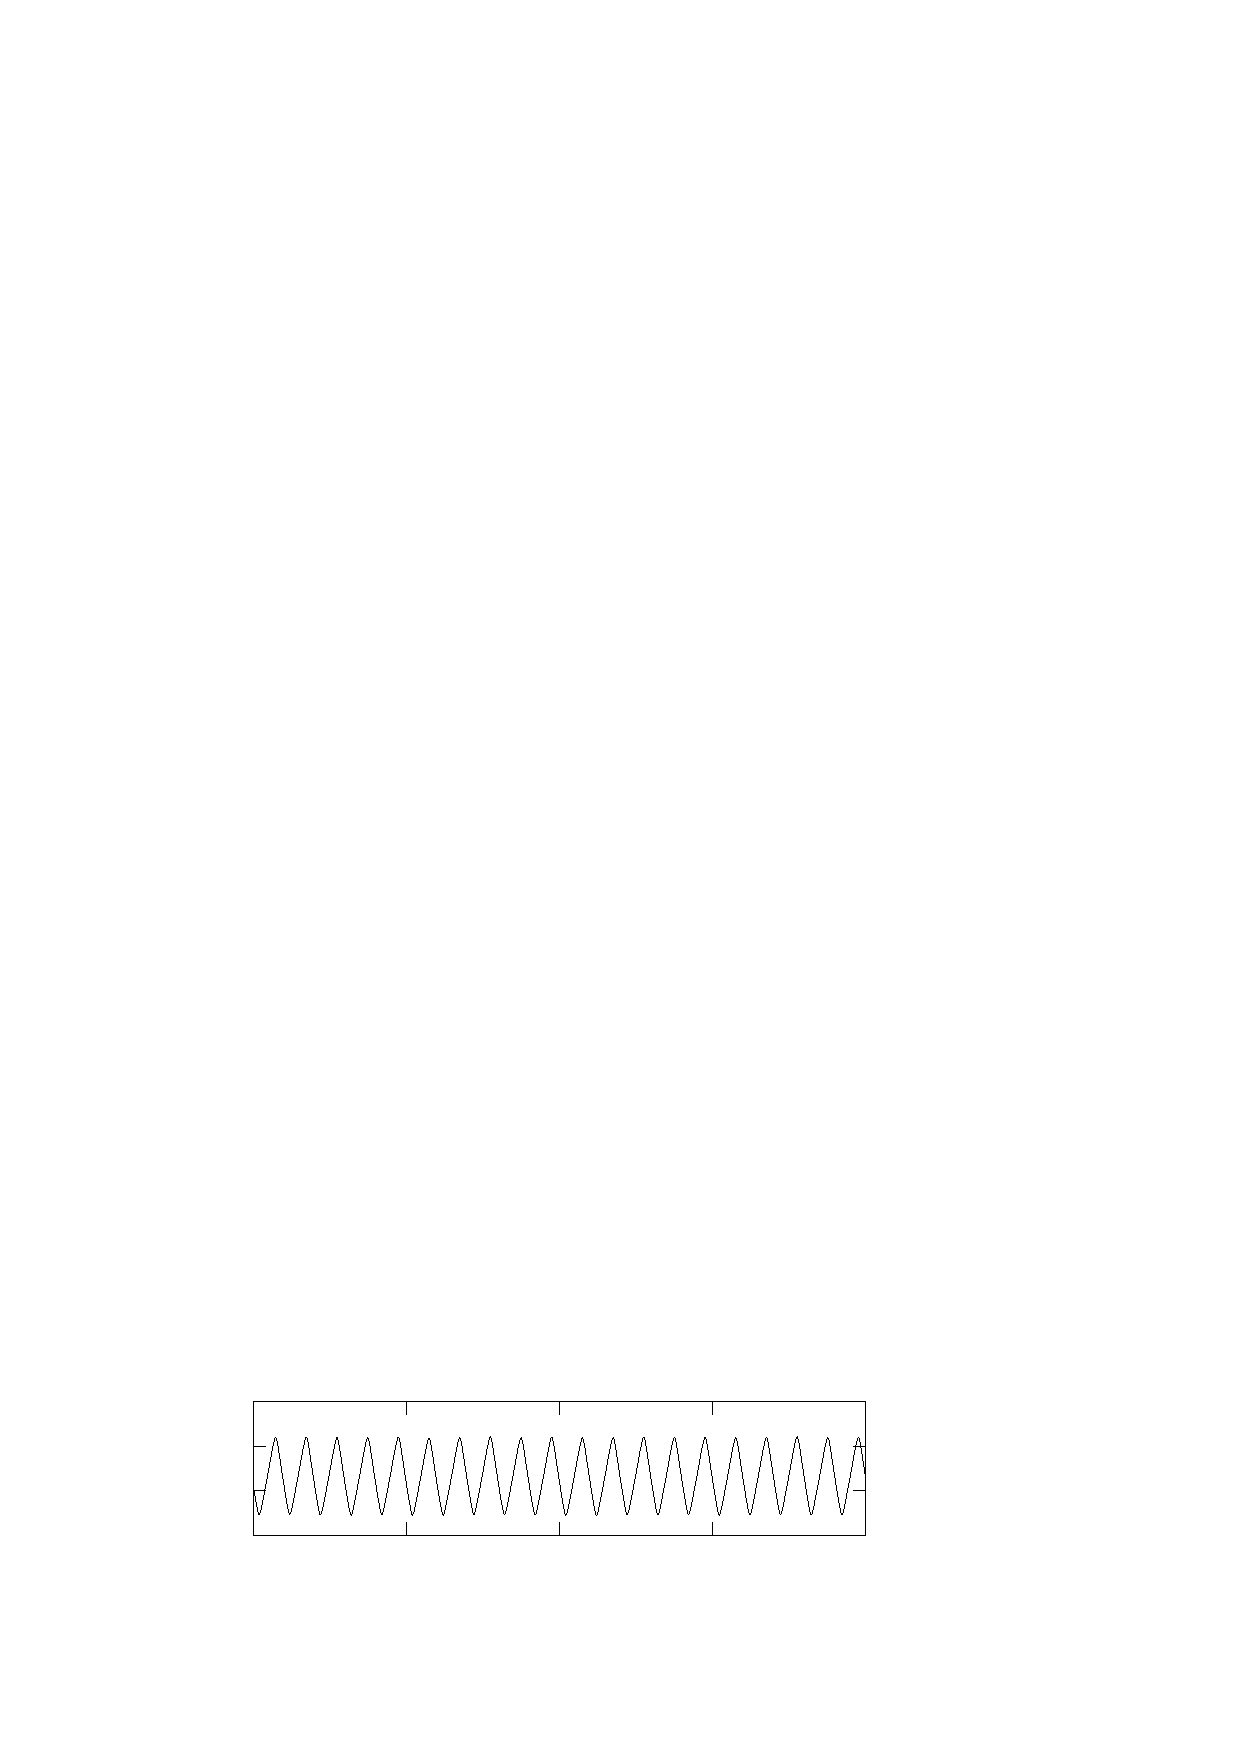
\includegraphics{rounded-barridorho1_2}%
%\end{picture}%
%\begingroup
%\setlength{\unitlength}{0.0200bp}%
%\begin{picture}(18000,5400)(0,0)%
%\put(2200,1650){\makebox(0,0)[r]{\strut{}1.26}}%
%\put(2200,2717){\makebox(0,0)[r]{\strut{}1.44}}%
%\put(2200,3783){\makebox(0,0)[r]{\strut{}1.62}}%
%\put(2200,4850){\makebox(0,0)[r]{\strut{}1.80}}%
%\put(2475,1100){\makebox(0,0){\strut{} 300}}%
%\put(6150,1100){\makebox(0,0){\strut{} 305}}%
%\put(9825,1100){\makebox(0,0){\strut{} 310}}%
%\put(13500,1100){\makebox(0,0){\strut{} 315}}%
%\put(17175,1100){\makebox(0,0){\strut{} 320}}%
%\put(550,3250){\rotatebox{90}{\makebox(0,0){\strut{}$y^\ast$}}}%
%\put(9825,275){\makebox(0,0){\strut{}$t^\ast$}}%
%\put(600,1000){\rotatebox{0}{\makebox(0,0){\strut{}(a)}}}%
%\end{picture}%
%\endgroup
%\endinput

%%GNUPLOT: LaTeX picture with Postscript
%\begin{picture}(0,0)%
%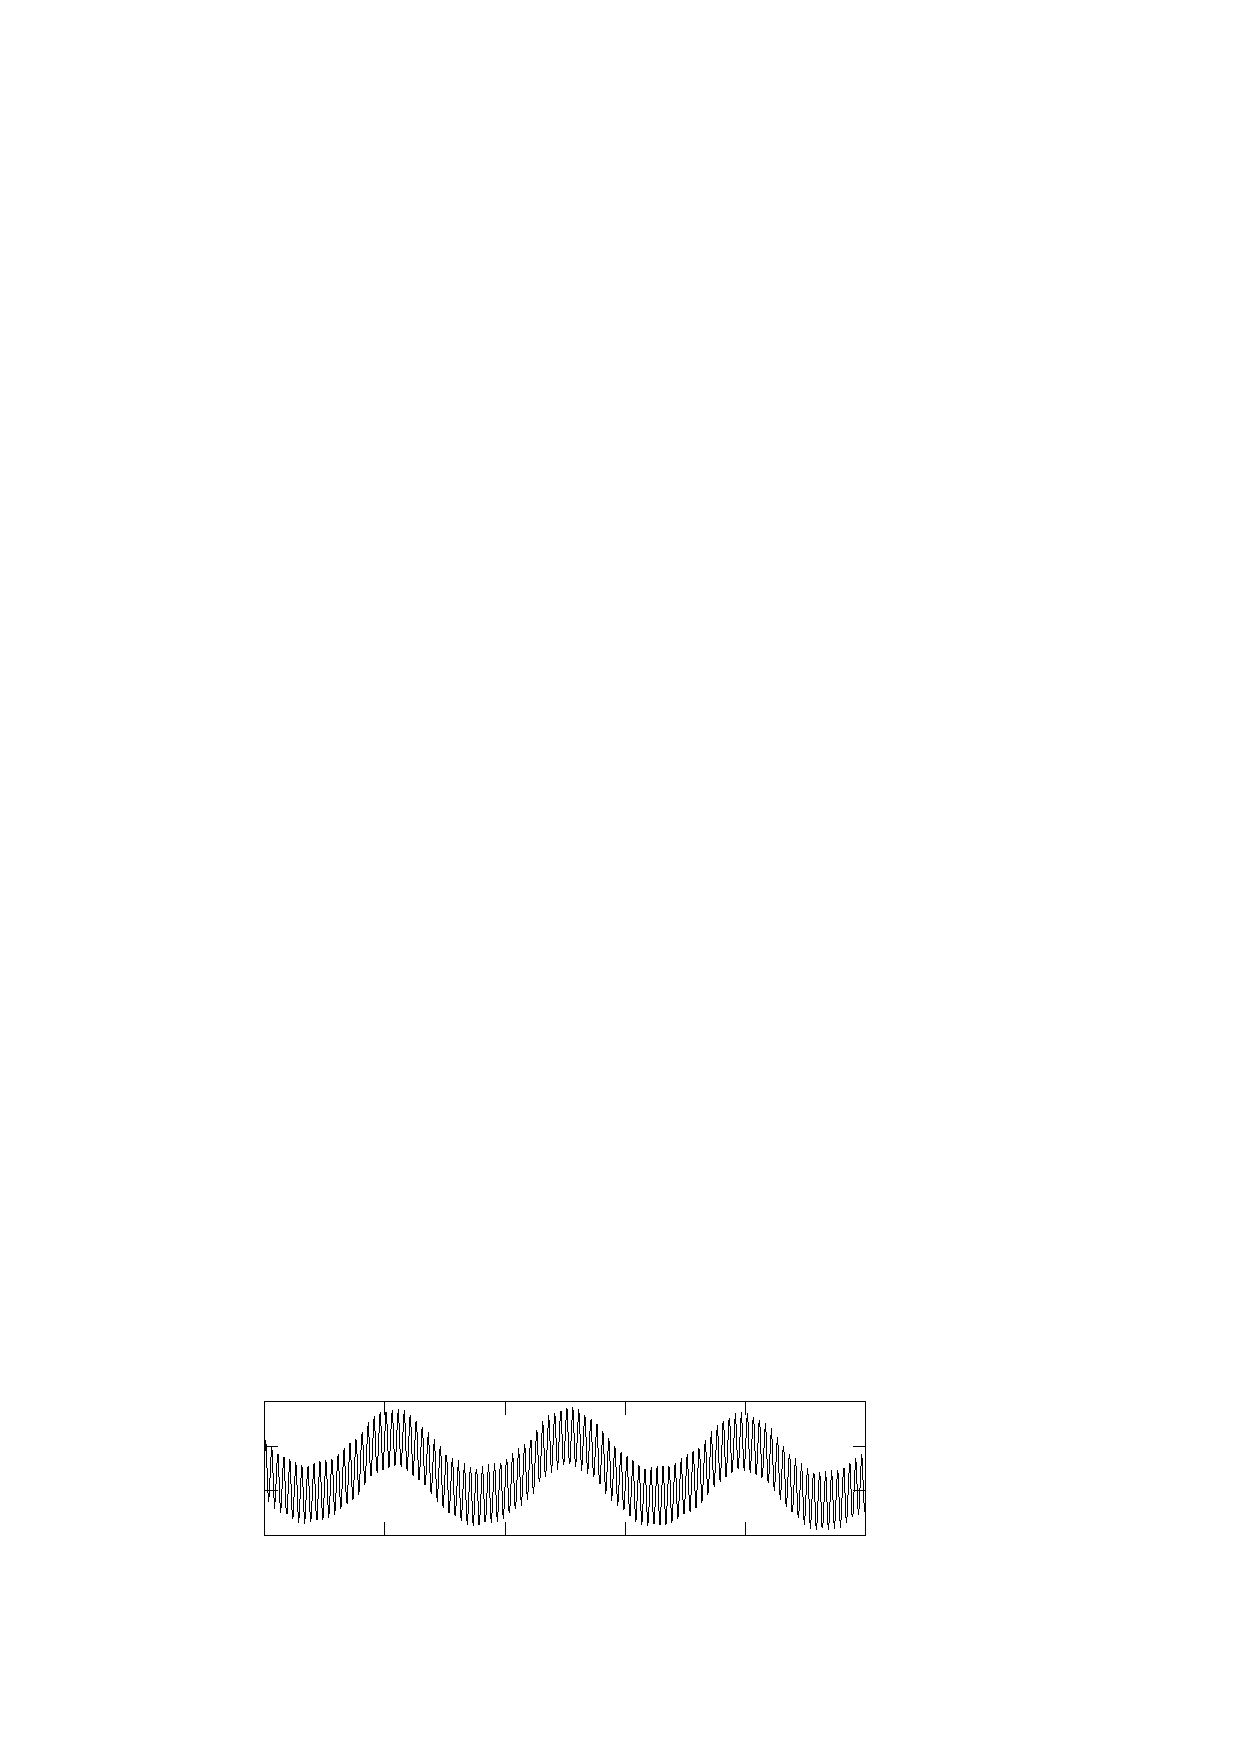
\includegraphics{rounded-barridorho30}%
%\end{picture}%
%\begingroup
%\setlength{\unitlength}{0.0200bp}%
%\begin{picture}(18000,5400)(0,0)%
%\put(2475,1650){\makebox(0,0)[r]{\strut{}1.410}}%
%\put(2475,2717){\makebox(0,0)[r]{\strut{}1.425}}%
%\put(2475,3783){\makebox(0,0)[r]{\strut{}1.440}}%
%\put(2475,4850){\makebox(0,0)[r]{\strut{}1.455}}%
%\put(2750,1100){\makebox(0,0){\strut{} 1800}}%
%\put(5635,1100){\makebox(0,0){\strut{} 1820}}%
%\put(8520,1100){\makebox(0,0){\strut{} 1840}}%
%\put(11405,1100){\makebox(0,0){\strut{} 1860}}%
%\put(14290,1100){\makebox(0,0){\strut{} 1880}}%
%\put(17175,1100){\makebox(0,0){\strut{} 1900}}%
%\put(550,3250){\rotatebox{90}{\makebox(0,0){\strut{}$y^\ast$}}}%
%\put(9962,275){\makebox(0,0){\strut{}$t^\ast$}}%
%\put(600,1000){\rotatebox{0}{\makebox(0,0){\strut{}(b)}}}%
%\end{picture}%
%\endgroup
%\endinput

%%GNUPLOT: LaTeX picture with Postscript
%\begin{picture}(0,0)%
%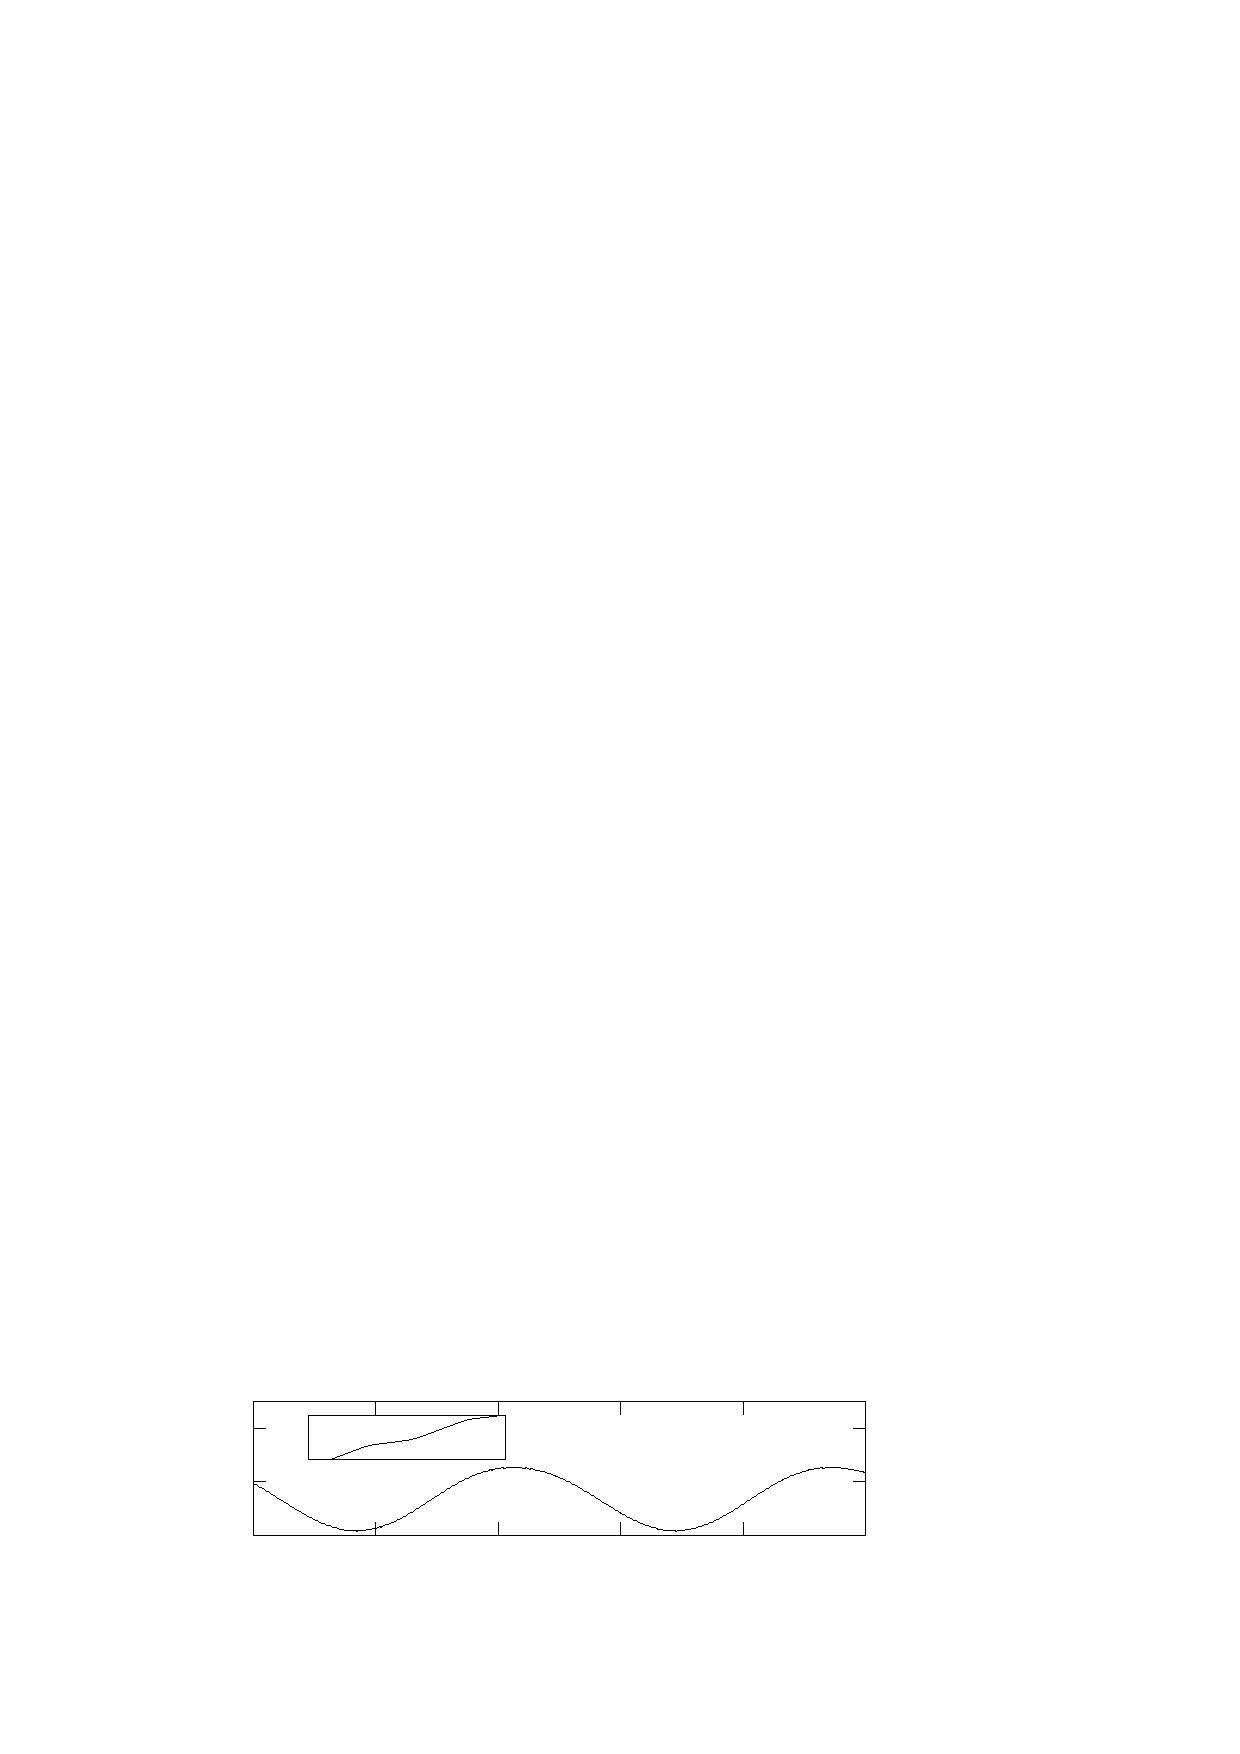
\includegraphics{rounded-barridorho60}%
%\end{picture}%
%\begingroup
%\setlength{\unitlength}{0.0200bp}%
%\begin{picture}(18000,5400)(0,0)%
%\put(2200,1650){\makebox(0,0)[r]{\strut{}0.80}}%
%\put(2200,2930){\makebox(0,0)[r]{\strut{}1.60}}%
%\put(2200,4210){\makebox(0,0)[r]{\strut{}2.40}}%
%\put(2475,1100){\makebox(0,0){\strut{} 1400}}%
%\put(5415,1100){\makebox(0,0){\strut{} 1420}}%
%\put(8355,1100){\makebox(0,0){\strut{} 1440}}%
%\put(11295,1100){\makebox(0,0){\strut{} 1460}}%
%\put(14235,1100){\makebox(0,0){\strut{} 1480}}%
%\put(17175,1100){\makebox(0,0){\strut{} 1500}}%
%\put(550,3250){\rotatebox{90}{\makebox(0,0){\strut{}$y^\ast$}}}%
%\put(9825,275){\makebox(0,0){\strut{}$t^\ast$}}%
%\put(3535,3476){\makebox(0,0)[r]{\strut{}1.4}}%
%\put(3535,4526){\makebox(0,0)[r]{\strut{}1.5}}%
%\put(3810,2926){\makebox(0,0){\strut{} 1430}}%
%\put(8535,2926){\makebox(0,0){\strut{} 1432}}%
%\put(600,1000){\rotatebox{0}{\makebox(0,0){\strut{}(c)}}}%
%\end{picture}%
%\endgroup
%\endinput

%%GNUPLOT: LaTeX picture with Postscript
%\begin{picture}(0,0)%
%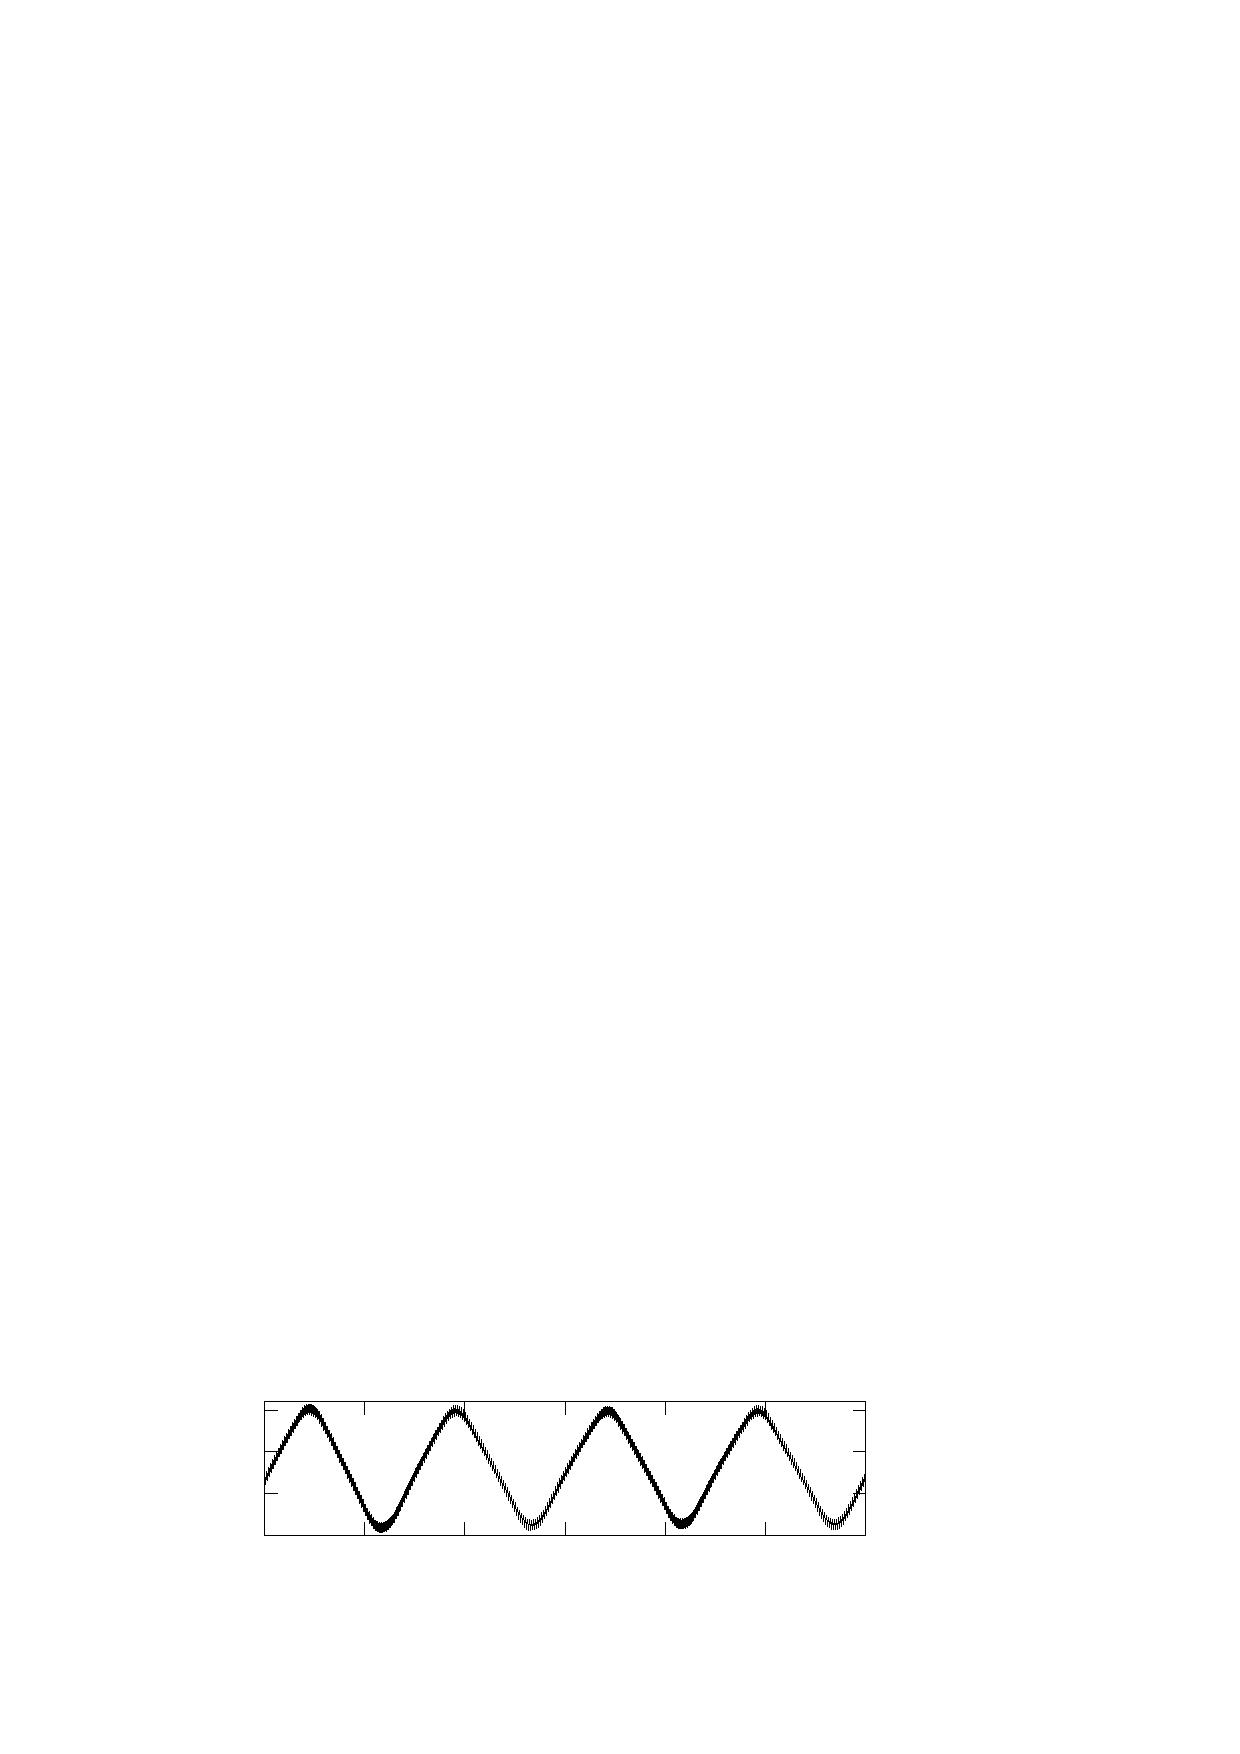
\includegraphics{rounded-barridorho153_6}%
%\end{picture}%
%\begingroup
%\setlength{\unitlength}{0.0200bp}%
%\begin{picture}(18000,5400)(0,0)%
%\put(2475,1650){\makebox(0,0)[r]{\strut{}1.020}}%
%\put(2475,2650){\makebox(0,0)[r]{\strut{}1.035}}%
%\put(2475,3650){\makebox(0,0)[r]{\strut{}1.050}}%
%\put(2475,4650){\makebox(0,0)[r]{\strut{}1.065}}%
%\put(2750,1100){\makebox(0,0){\strut{} 3000}}%
%\put(5154,1100){\makebox(0,0){\strut{} 3050}}%
%\put(7558,1100){\makebox(0,0){\strut{} 3100}}%
%\put(9963,1100){\makebox(0,0){\strut{} 3150}}%
%\put(12367,1100){\makebox(0,0){\strut{} 3200}}%
%\put(14771,1100){\makebox(0,0){\strut{} 3250}}%
%\put(17175,1100){\makebox(0,0){\strut{} 3300}}%
%\put(550,3250){\rotatebox{90}{\makebox(0,0){\strut{}$y^\ast$}}}%
%\put(9962,275){\makebox(0,0){\strut{}$t^\ast$}}%
%\put(600,1000){\makebox(0,0){\strut{}(d)}}%
%\end{picture}%
%\endgroup
%\endinput

\caption{\label{fig:paths-rounded}
Posici'on vertical de la part'icula s'olida sobre el tiempo en la cavidad redondeada para
(a) $\rho_p/\rho_f = 2$,
(b) $\rho_p/\rho_f = 50$,
(c) $\rho_p/\rho_f = 100$
y
(d) $\rho_p/\rho_f =256$.
}
\end{figure}

\begin{figure} 
%\put(600,2550){\rotatebox{90}{\makebox(0,0){\strut{}(a)}}}%
%%GNUPLOT: LaTeX picture with Postscript
%\begin{picture}(0,0)%
%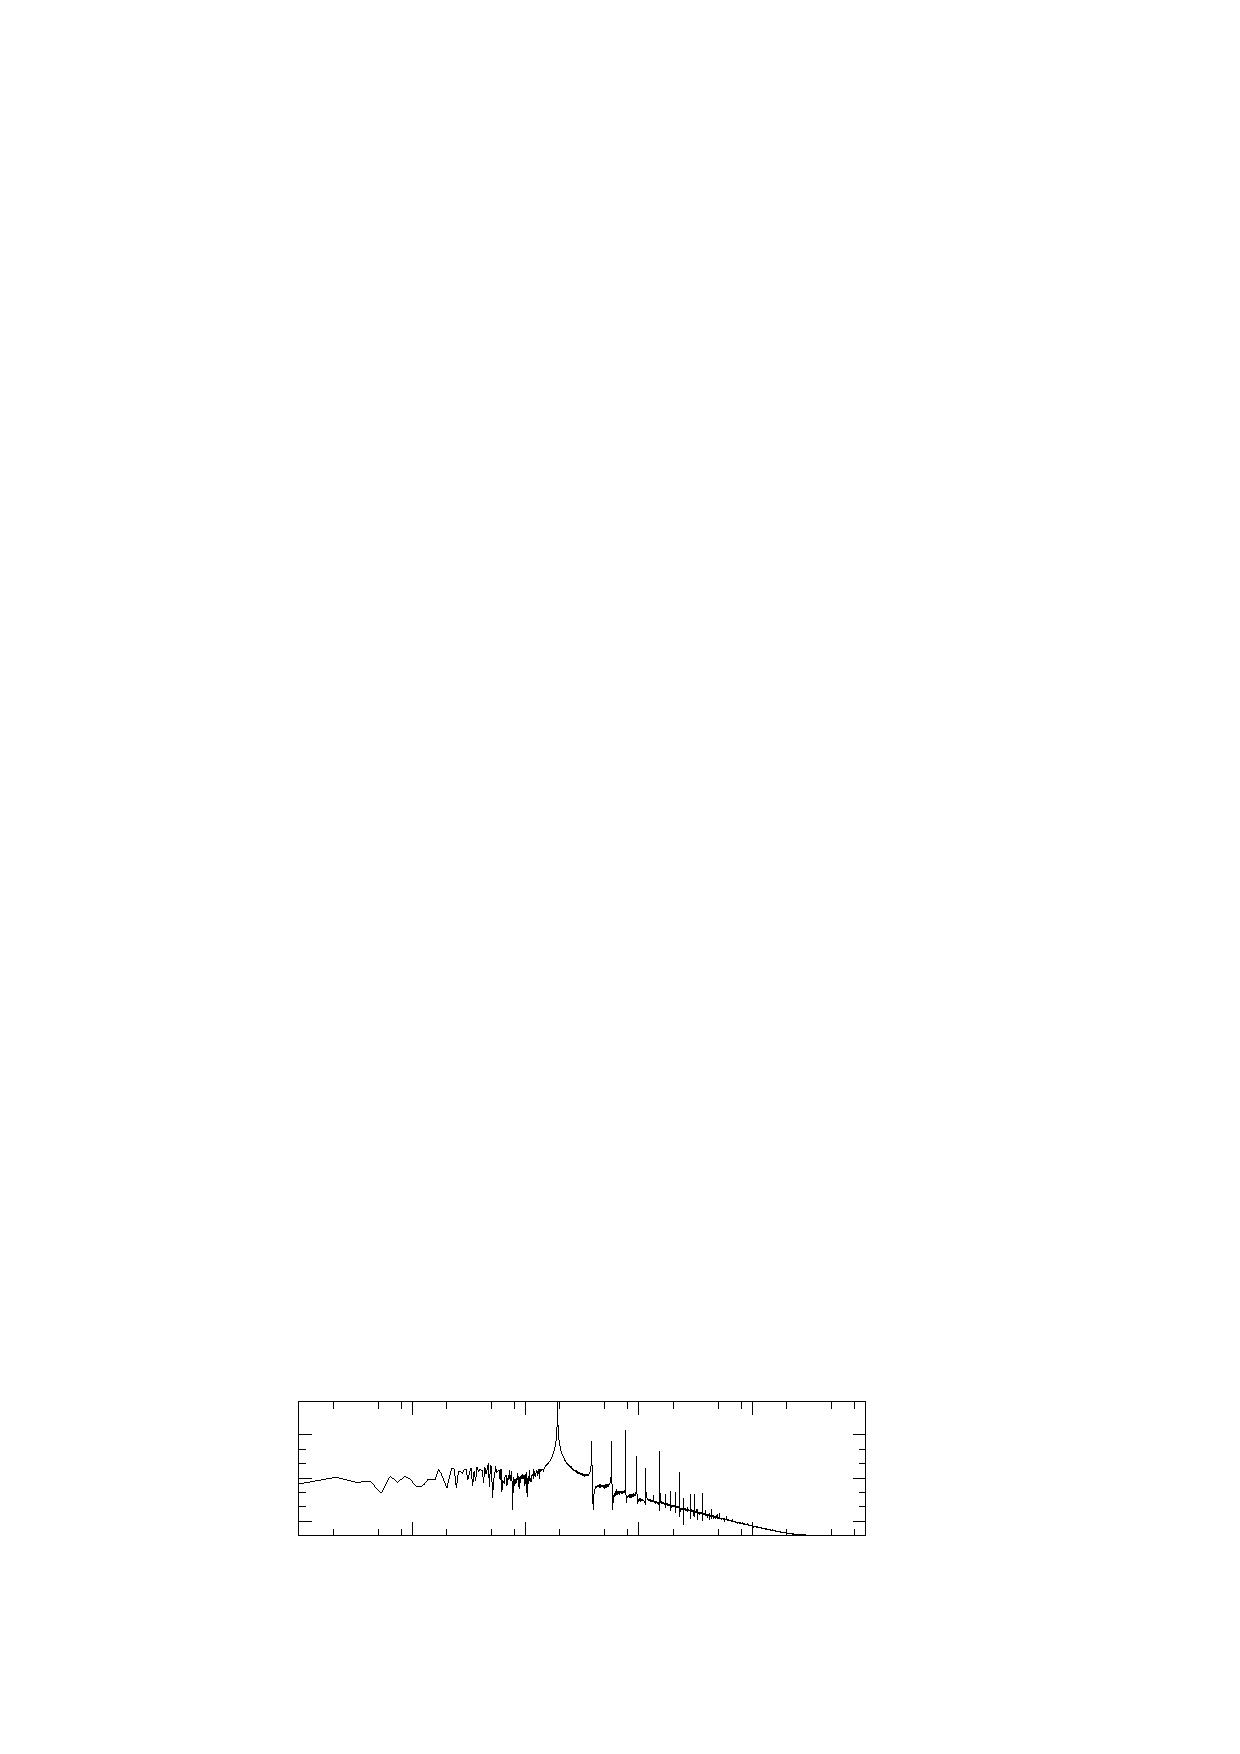
\includegraphics{rounded-barridorho1_2-spectrum}%
%\end{picture}%
%\begingroup
%\setlength{\unitlength}{0.0200bp}%
%\begin{picture}(18000,5400)(0,0)%
%\put(3300,1985){\makebox(0,0)[r]{\strut{}1.00e-12}}%
%\put(3300,3023){\makebox(0,0)[r]{\strut{}1.00e-09}}%
%\put(3300,4062){\makebox(0,0)[r]{\strut{}1.00e-06}}%
%\put(3575,1100){\makebox(0,0){\strut{} 1e-04}}%
%\put(6295,1100){\makebox(0,0){\strut{} 0.001}}%
%\put(9015,1100){\makebox(0,0){\strut{} 0.01}}%
%\put(11735,1100){\makebox(0,0){\strut{} 0.1}}%
%\put(14455,1100){\makebox(0,0){\strut{} 1}}%
%\put(17175,1100){\makebox(0,0){\strut{} 10}}%
%\put(550,3250){\rotatebox{90}{\makebox(0,0){\strut{}$PSD$}}}%
%\put(10375,275){\makebox(0,0){\strut{}$\omega$}}%
%\put(600,1000){\makebox(0,0){\strut{}(a)}}%
%\end{picture}%
%\endgroup
%\endinput

%%GNUPLOT: LaTeX picture with Postscript
%\begin{picture}(0,0)%
%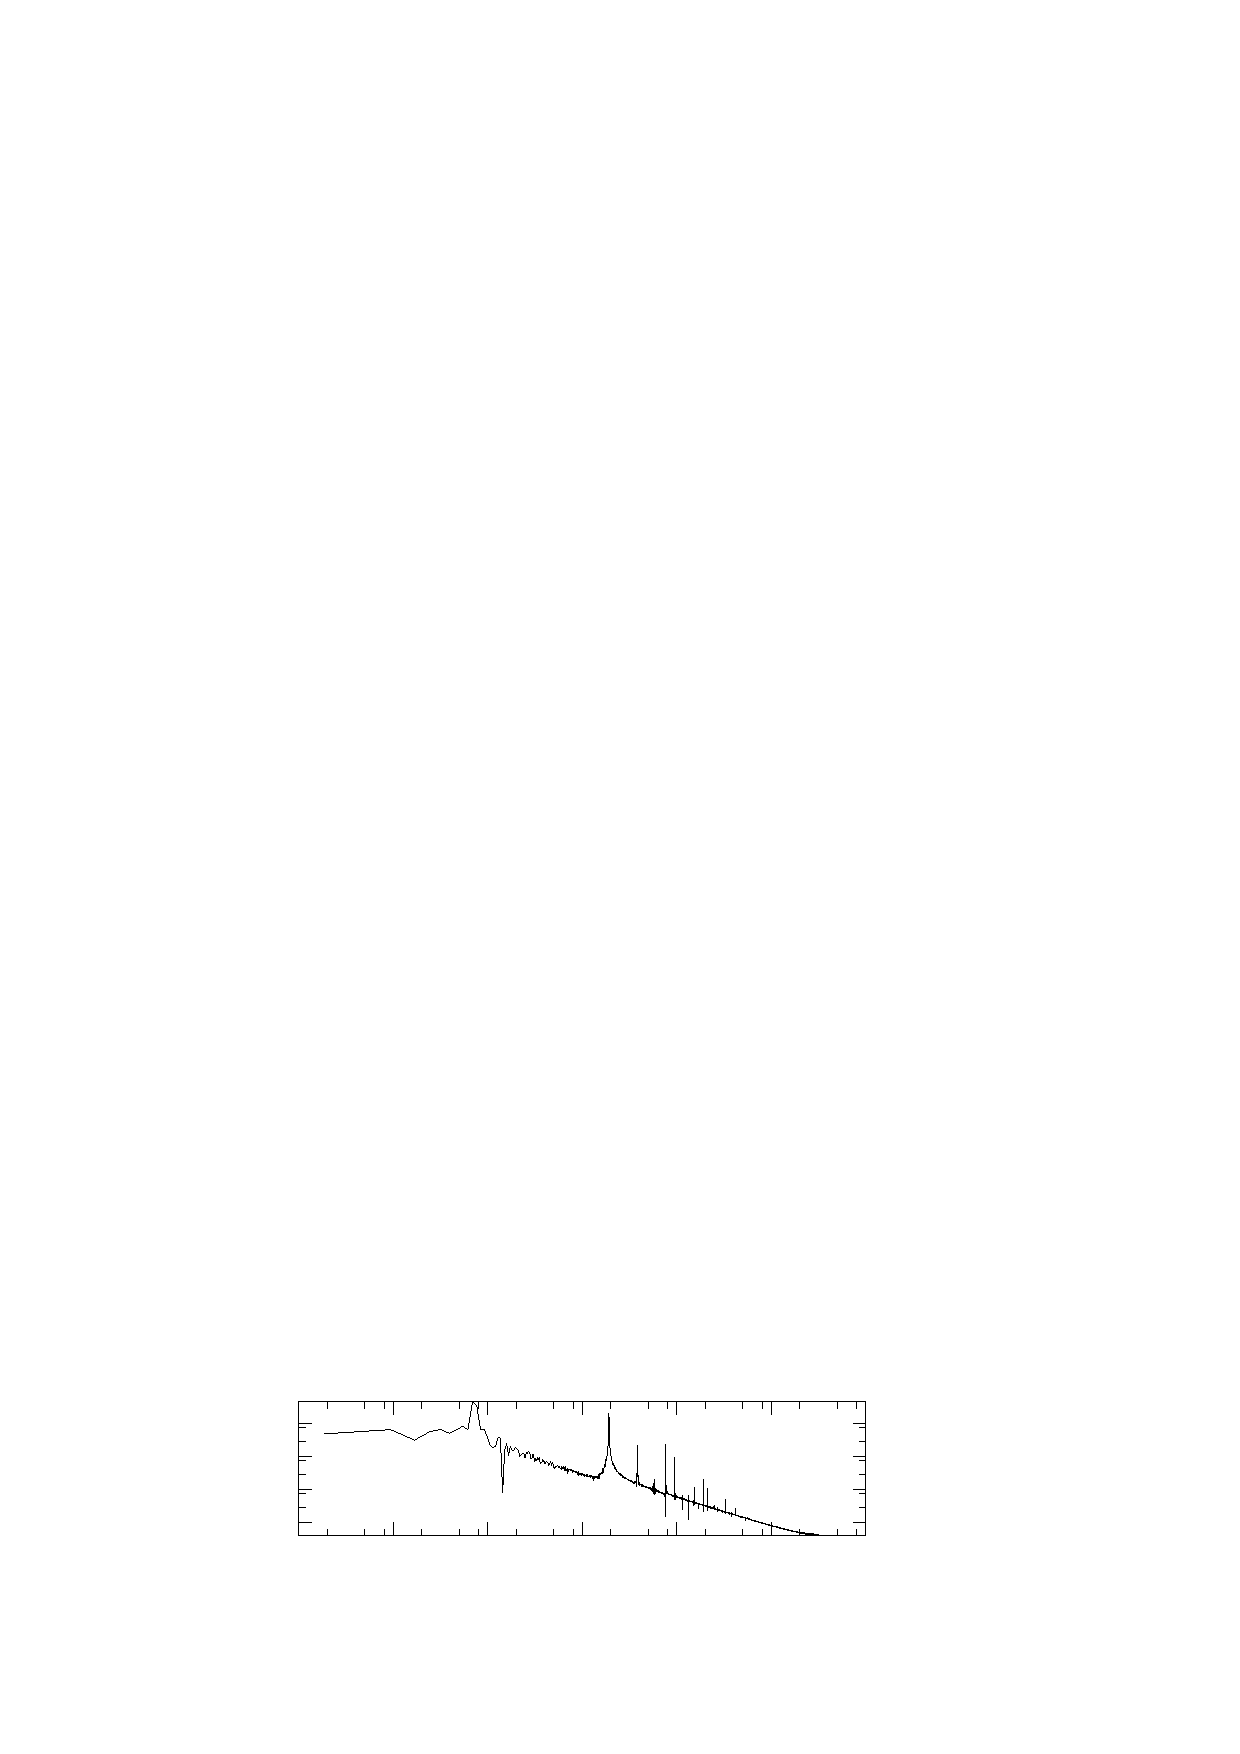
\includegraphics{rounded-barridorho30-spectrum}%
%\end{picture}%
%\begingroup
%\setlength{\unitlength}{0.0200bp}%
%\begin{picture}(18000,5400)(0,0)%
%\put(3300,1960){\makebox(0,0)[r]{\strut{}1.56e-14}}%
%\put(3300,2755){\makebox(0,0)[r]{\strut{}3.13e-12}}%
%\put(3300,3549){\makebox(0,0)[r]{\strut{}6.25e-10}}%
%\put(3300,4343){\makebox(0,0)[r]{\strut{}1.25e-07}}%
%\put(3575,1100){\makebox(0,0){\strut{} 1e-05}}%
%\put(5842,1100){\makebox(0,0){\strut{} 1e-04}}%
%\put(8108,1100){\makebox(0,0){\strut{} 0.001}}%
%\put(10375,1100){\makebox(0,0){\strut{} 0.01}}%
%\put(12642,1100){\makebox(0,0){\strut{} 0.1}}%
%\put(14908,1100){\makebox(0,0){\strut{} 1}}%
%\put(17175,1100){\makebox(0,0){\strut{} 10}}%
%\put(550,3250){\rotatebox{90}{\makebox(0,0){\strut{}$PSD$}}}%
%\put(10375,275){\makebox(0,0){\strut{}$\omega$}}%
%\put(600,1000){\makebox(0,0){\strut{}(b)}}%
%\end{picture}%
%\endgroup
%\endinput

%%GNUPLOT: LaTeX picture with Postscript
%\begin{picture}(0,0)%
%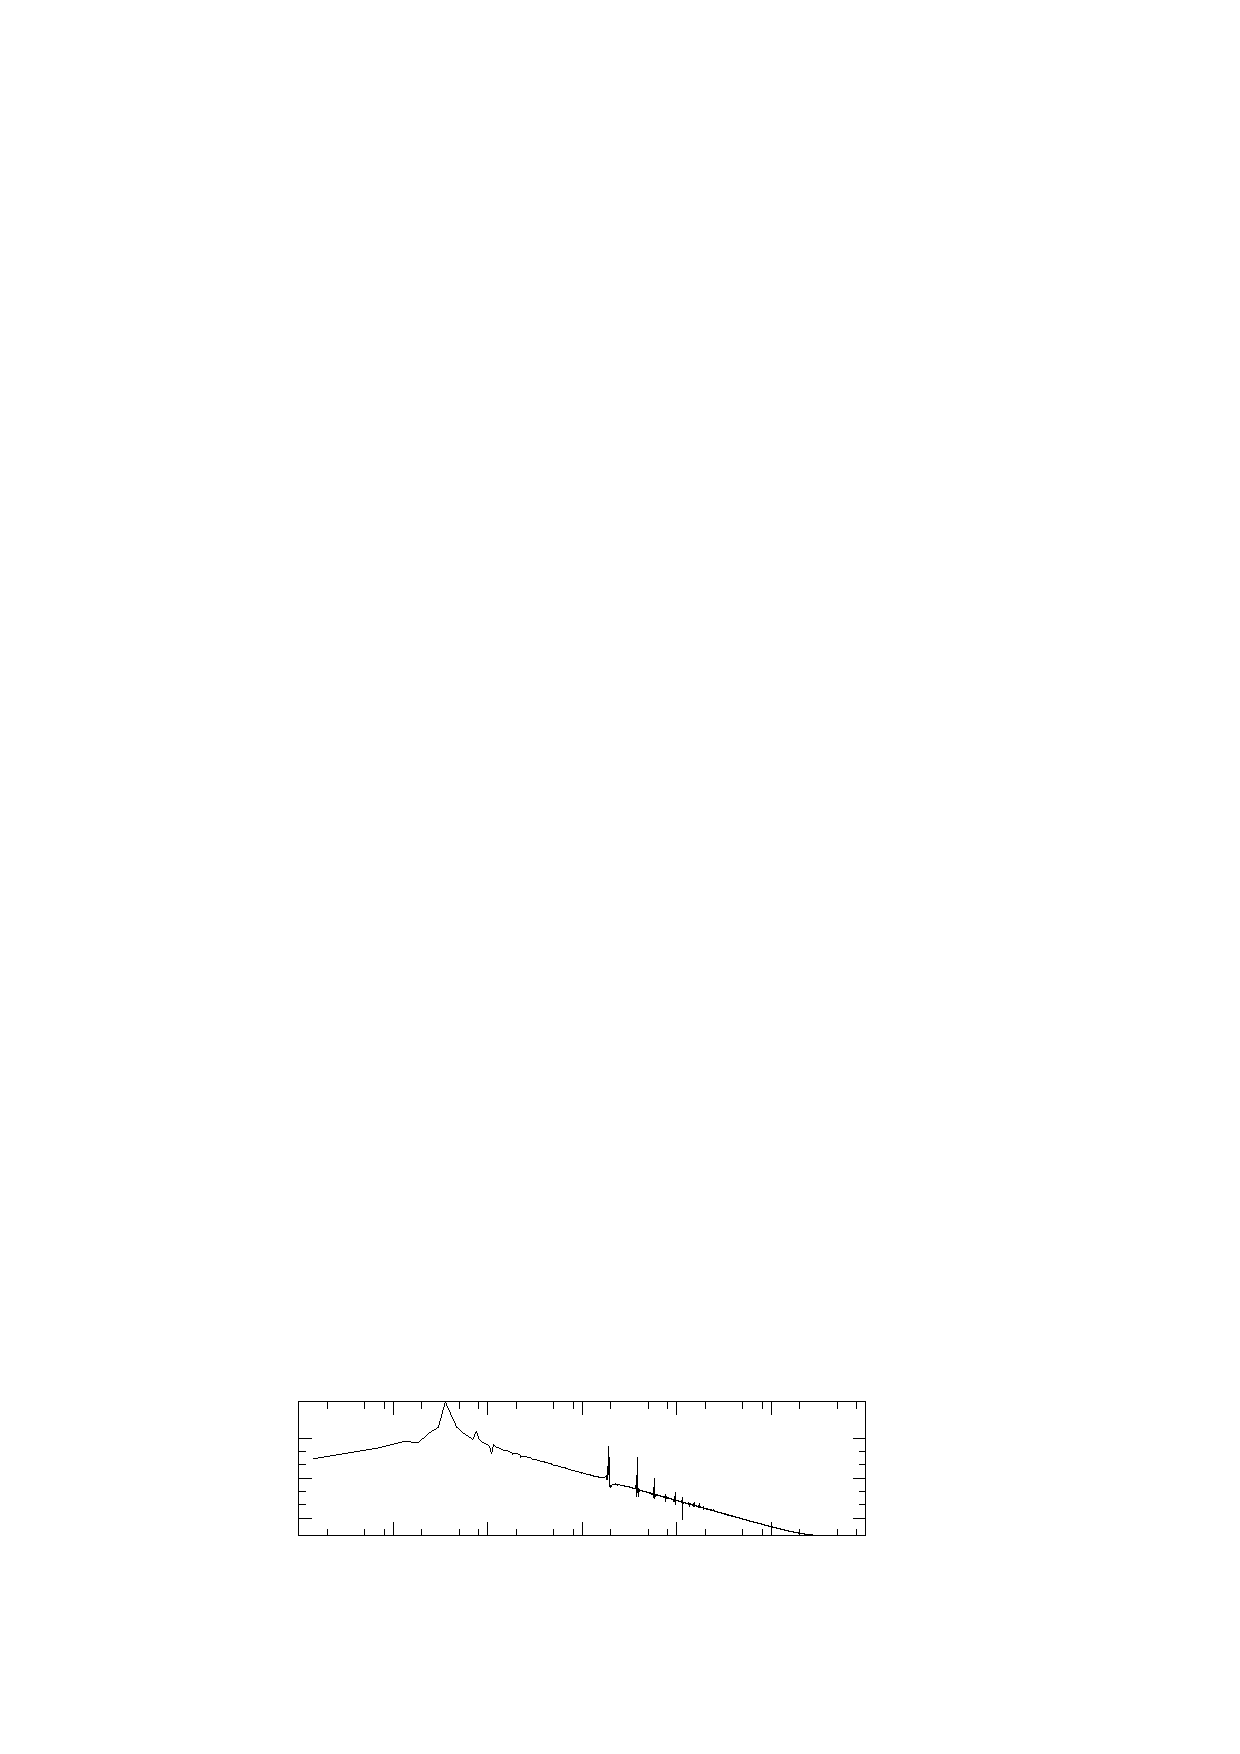
\includegraphics{rounded-barridorho60-spectrum}%
%\end{picture}%
%\begingroup
%\setlength{\unitlength}{0.0200bp}%
%\begin{picture}(18000,5400)(0,0)%
%\put(3300,2056){\makebox(0,0)[r]{\strut{}1.00e-12}}%
%\put(3300,3019){\makebox(0,0)[r]{\strut{}1.00e-09}}%
%\put(3300,3982){\makebox(0,0)[r]{\strut{}1.00e-06}}%
%\put(3575,1100){\makebox(0,0){\strut{} 1e-05}}%
%\put(5842,1100){\makebox(0,0){\strut{} 1e-04}}%
%\put(8108,1100){\makebox(0,0){\strut{} 0.001}}%
%\put(10375,1100){\makebox(0,0){\strut{} 0.01}}%
%\put(12642,1100){\makebox(0,0){\strut{} 0.1}}%
%\put(14908,1100){\makebox(0,0){\strut{} 1}}%
%\put(17175,1100){\makebox(0,0){\strut{} 10}}%
%\put(550,3250){\rotatebox{90}{\makebox(0,0){\strut{}$PSD$}}}%
%\put(10375,275){\makebox(0,0){\strut{}$\omega$}}%
%\put(600,1000){\makebox(0,0){\strut{}(c)}}%
%\end{picture}%
%\endgroup
%\endinput

%%GNUPLOT: LaTeX picture with Postscript
%\begin{picture}(0,0)%
%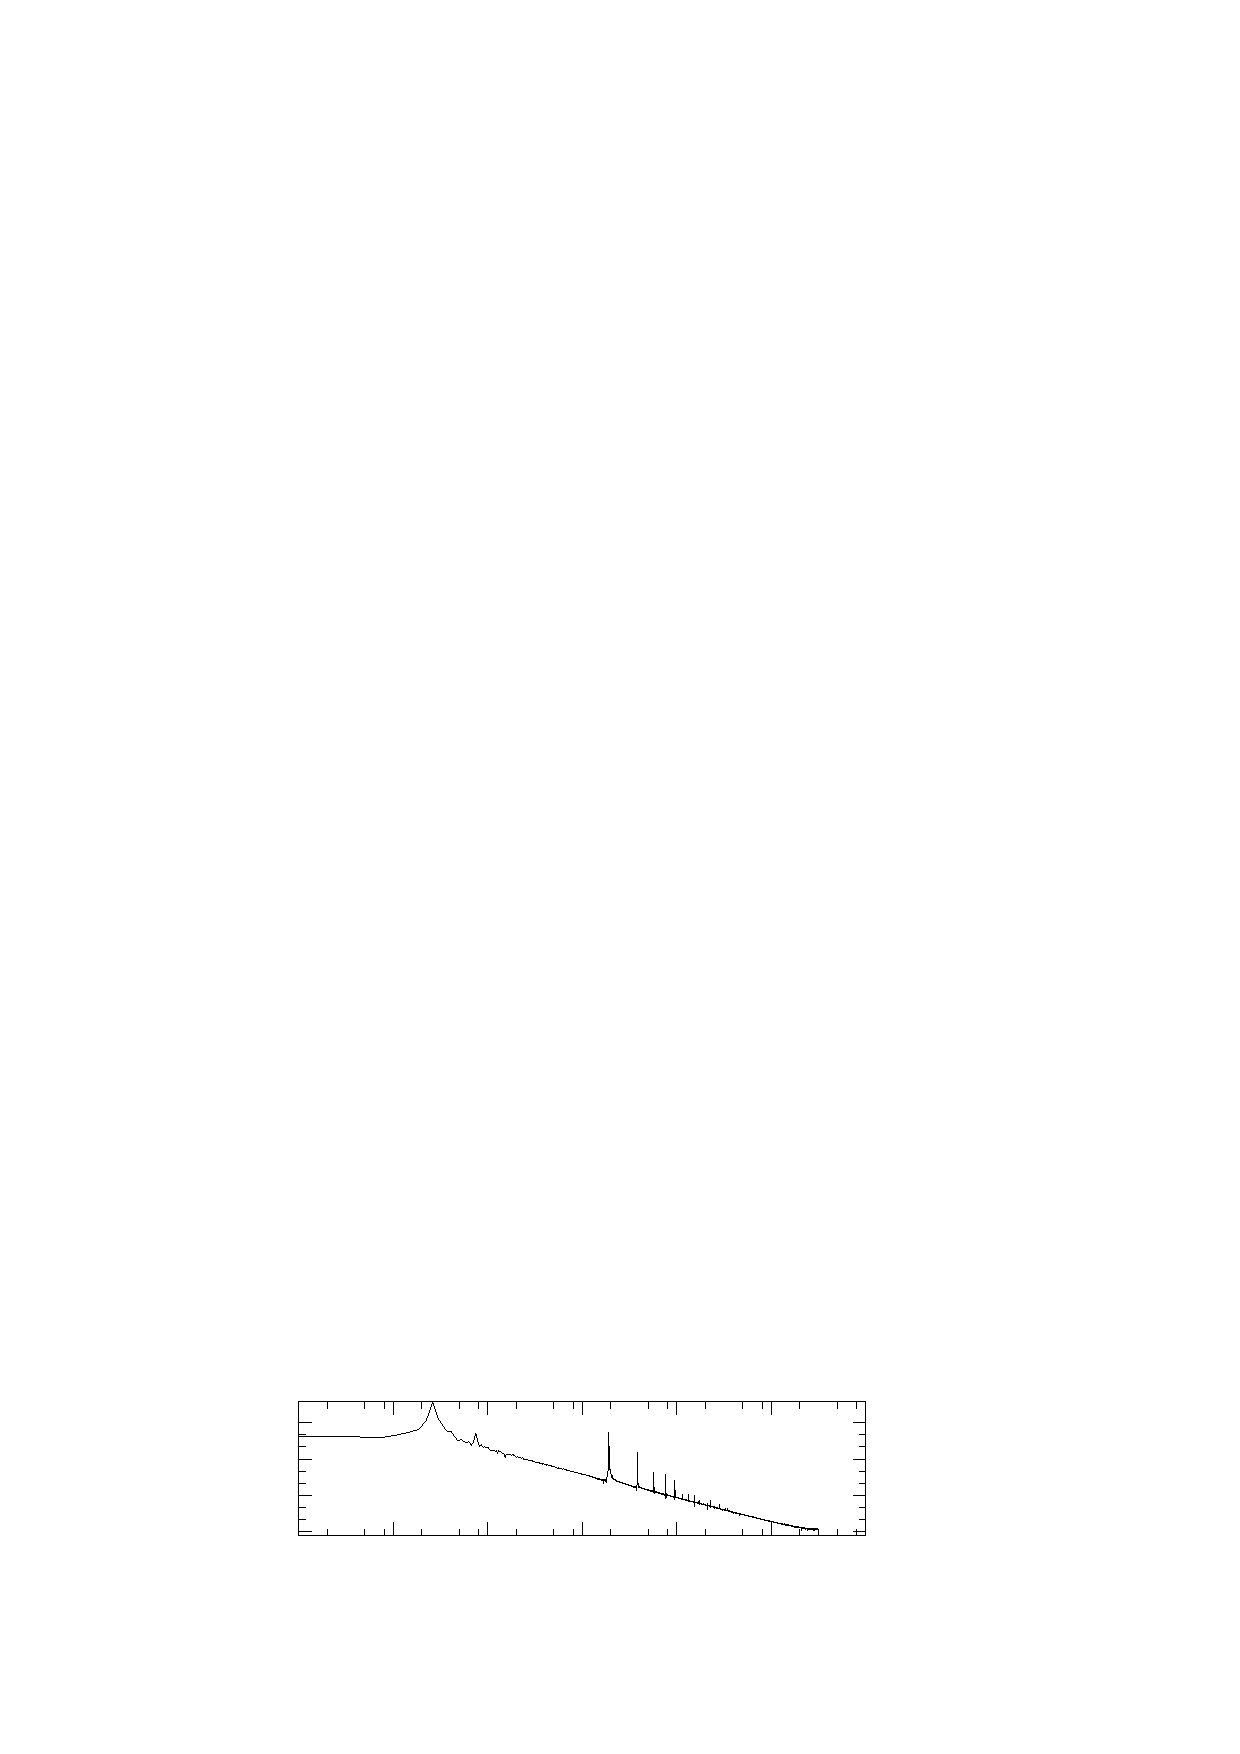
\includegraphics{rounded-barridorho153_6-spectrum}%
%\end{picture}%
%\begingroup
%\setlength{\unitlength}{0.0200bp}%
%\begin{picture}(18000,5400)(0,0)%
%\put(3300,1729){\makebox(0,0)[r]{\strut{}1.00e-15}}%
%\put(3300,2605){\makebox(0,0)[r]{\strut{}1.00e-12}}%
%\put(3300,3480){\makebox(0,0)[r]{\strut{}1.00e-09}}%
%\put(3300,4356){\makebox(0,0)[r]{\strut{}1.00e-06}}%
%\put(3575,1100){\makebox(0,0){\strut{} 1e-05}}%
%\put(5842,1100){\makebox(0,0){\strut{} 1e-04}}%
%\put(8108,1100){\makebox(0,0){\strut{} 0.001}}%
%\put(10375,1100){\makebox(0,0){\strut{} 0.01}}%
%\put(12642,1100){\makebox(0,0){\strut{} 0.1}}%
%\put(14908,1100){\makebox(0,0){\strut{} 1}}%
%\put(17175,1100){\makebox(0,0){\strut{} 10}}%
%\put(550,3250){\rotatebox{90}{\makebox(0,0){\strut{}$PSD$}}}%
%\put(600,1000){\makebox(0,0){\strut{}(d)}}%
%\end{picture}%
%\endgroup
%\endinput

\caption{\label{fig:spectrum-rounded}
Espectro de potencia del movimiento vertical de la part'icula s'olida sobre el tiempo en la cavidad redondeada para
(a) $\rho_p/\rho_f = 2$,
(b) $\rho_p/\rho_f = 50$,
(c) $\rho_p/\rho_f = 100$
y
(d) $\rho_p/\rho_f =256$.
Los espectros de potencia corresponden a los de las figuras~\ref{fig:paths-rounded} (a), (b), (c) y (d). 
}
\end{figure}

La cavidad redondeada presenta un comportamiento m'as complejo que la plana. 
En la figura~\ref{fig:paths-rounded} (a) mostramos a la part'icula oscilando verticalmente con 
frecuencia de la fuente ac'ustica, como podemos observar de la figura~\ref{fig:spectrum-rounded} (a).
En la  figura~\ref{fig:paths-rounded} (b) aparece una segunda frecuencia menor que la frecuencia
de la fuente ac'ustica, como podemos comprobar de la figura~\ref{fig:spectrum-rounded} (b).
Adem'as la amplitud de la oscilaci'on es un orden de magnitud menor que en el caso anterior.
Cuando la amplitud de la oscilaci'on es m'axima, la amplitud de la oscilaci'on debida a la
frecuencia de la fuente ac'ustica es peque~na, como mostramos en la figura~\ref{fig:paths-rounded} (c)
y su inserto. En la figura~\ref{fig:spectrum-rounded} (c) mostramos las frecuencias dominantes 
localizadas por  los picos del espectro de potencias. En la figura~\ref{fig:paths-rounded} (d) observamos 
otra vez que  el movimiento vertical de la part'icula tiene dos frecuencias, como confirmamos de la 
figura~\ref{fig:spectrum-rounded} (d), donde aparecen las dos frecuencias dominantes con sus arm'onicos.








\begin{figure} 
%GNUPLOT: LaTeX picture with Postscript
\begin{picture}(0,0)%
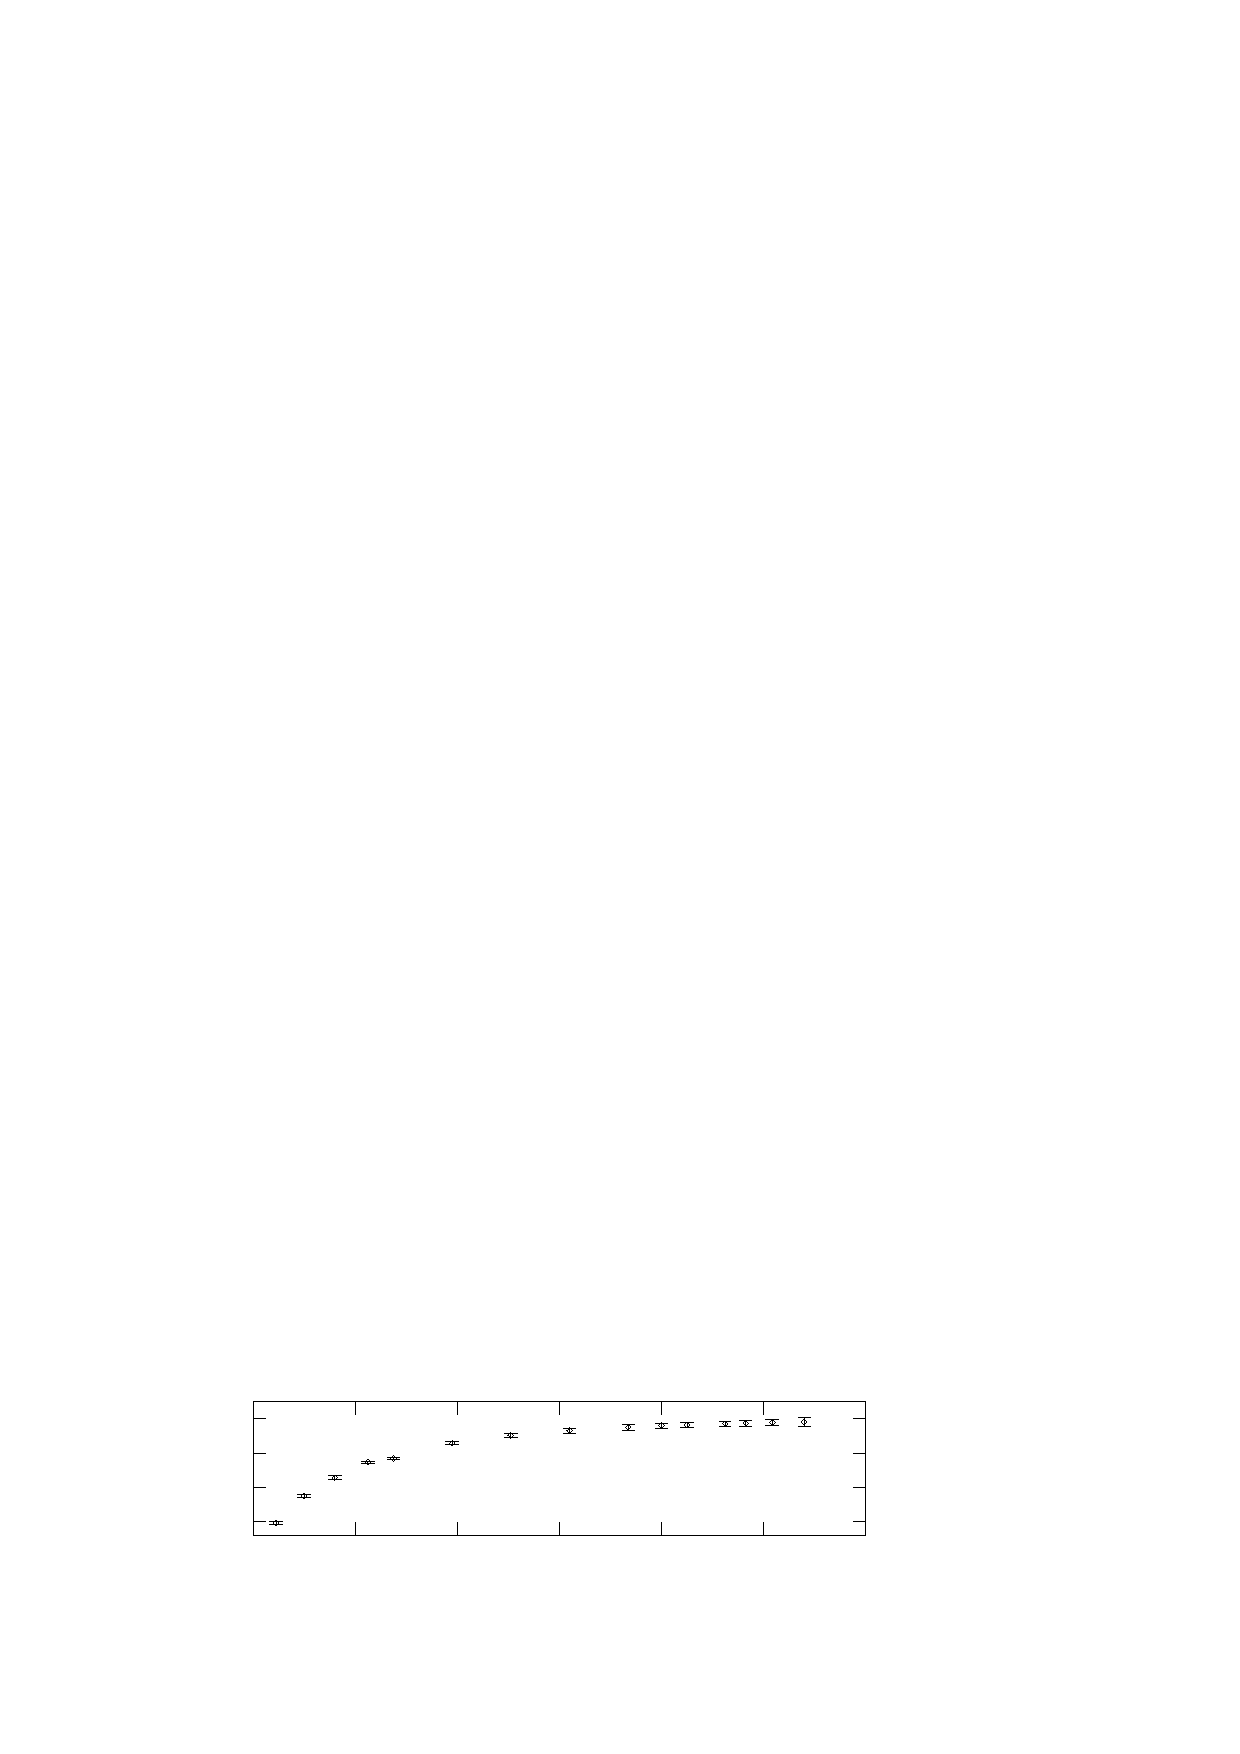
\includegraphics{eps/Fo-equilibrium-amplitud-flat}%
\end{picture}%
\begingroup
\setlength{\unitlength}{0.0200bp}%
\begin{picture}(18000,5400)(0,0)%
\put(2200,1990){\makebox(0,0)[r]{\strut{}1.20}}%
\put(2200,2807){\makebox(0,0)[r]{\strut{}1.32}}%
\put(2200,3624){\makebox(0,0)[r]{\strut{}1.44}}%
\put(2200,4441){\makebox(0,0)[r]{\strut{}1.56}}%
\put(2475,1100){\makebox(0,0){\strut{}0.004}}%
\put(4925,1100){\makebox(0,0){\strut{}0.006}}%
\put(7375,1100){\makebox(0,0){\strut{}0.008}}%
\put(9825,1100){\makebox(0,0){\strut{}0.010}}%
\put(12275,1100){\makebox(0,0){\strut{}0.012}}%
\put(14725,1100){\makebox(0,0){\strut{}0.014}}%
\put(17175,1100){\makebox(0,0){\strut{}0.016}}%
\put(550,3250){\rotatebox{90}{\makebox(0,0){\strut{}$y_{es}^\ast$}}}%
\put(9825,275){\makebox(0,0){\strut{}$P^\ast$}}%
\put(600,1000){\makebox(0,0)[r]{\strut{}(a)}}%
\end{picture}%
\endgroup
\endinput

%GNUPLOT: LaTeX picture with Postscript
\begin{picture}(0,0)%
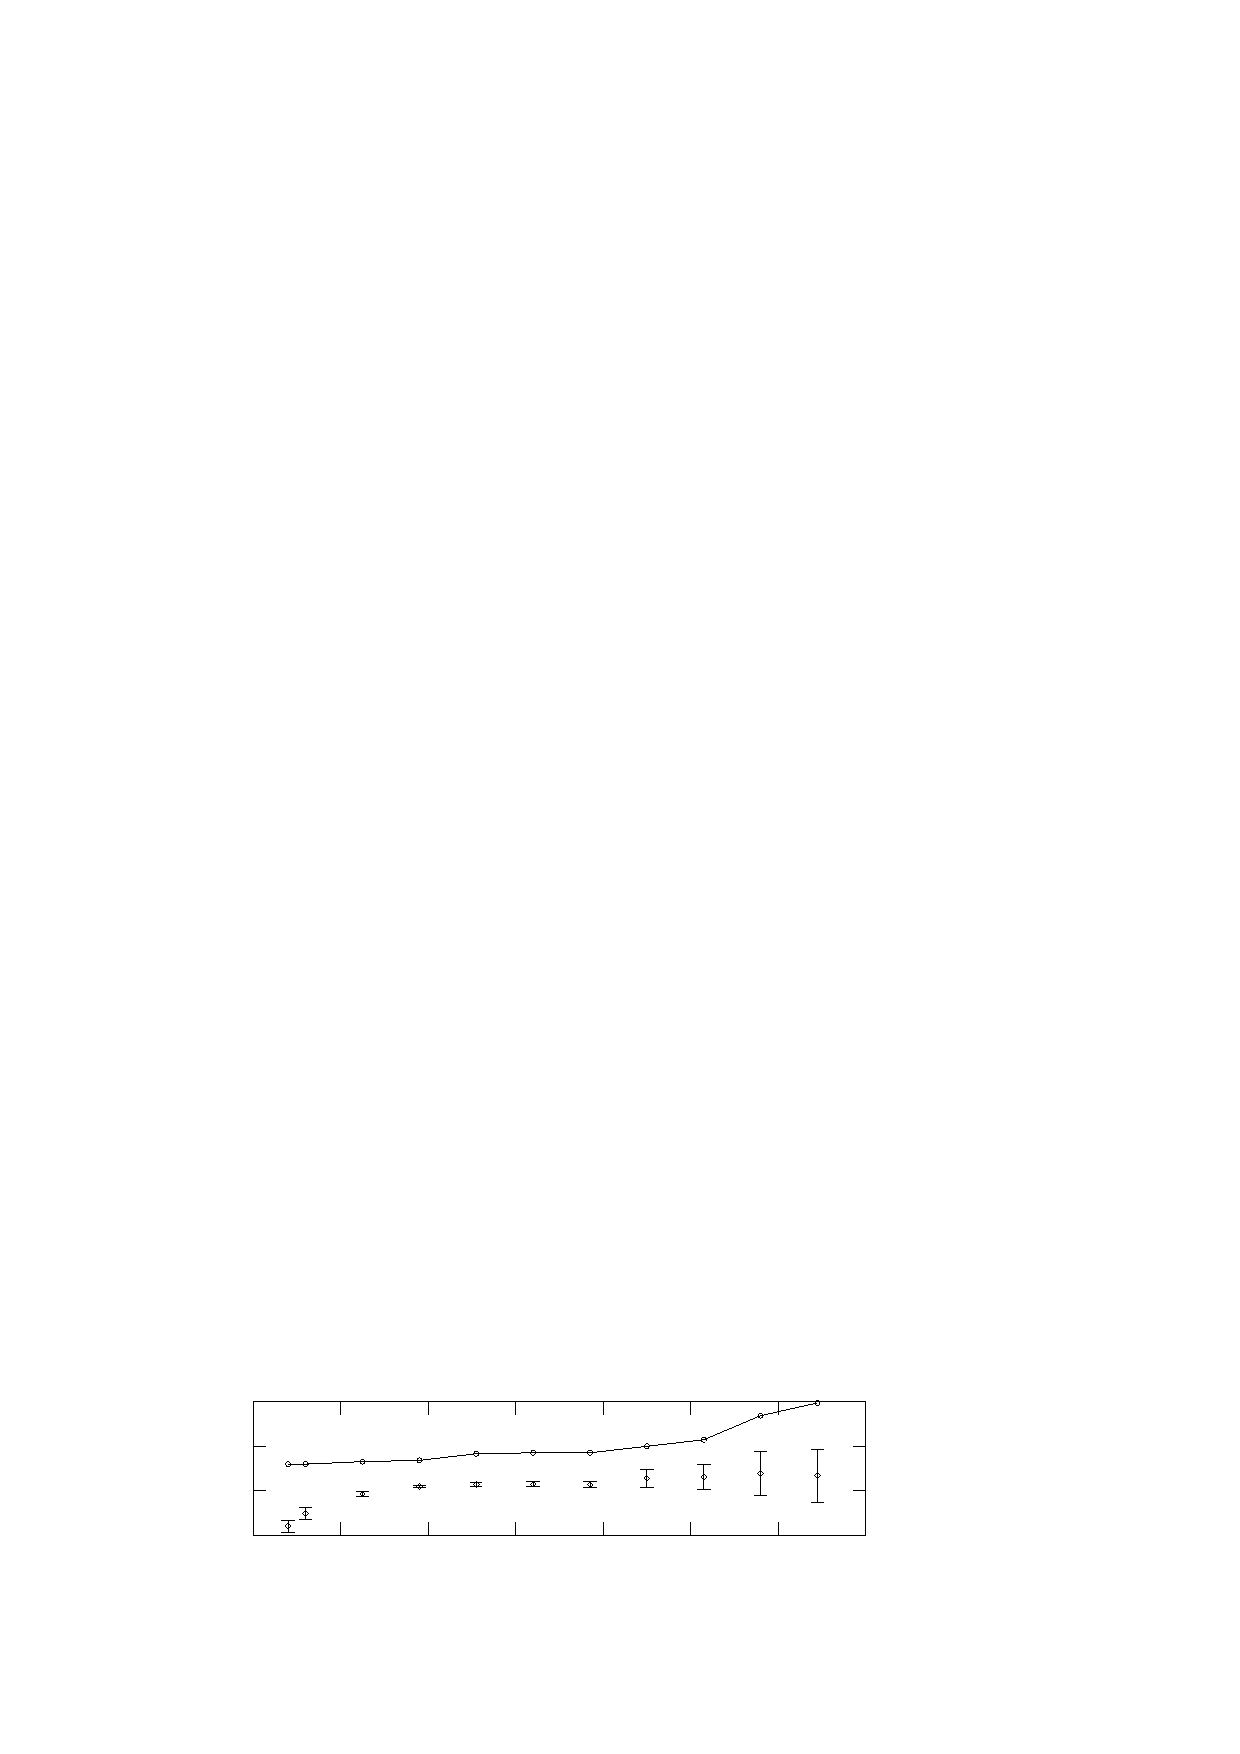
\includegraphics{Fo-equilibrium-amplitud-rounded}%
\end{picture}%
\begingroup
\setlength{\unitlength}{0.0200bp}%
\begin{picture}(18000,5400)(0,0)%
\put(2200,1650){\makebox(0,0)[r]{\strut{}1.05}}%
\put(2200,2717){\makebox(0,0)[r]{\strut{}1.40}}%
\put(2200,3783){\makebox(0,0)[r]{\strut{}1.75}}%
\put(2200,4850){\makebox(0,0)[r]{\strut{}2.10}}%
\put(2475,1100){\makebox(0,0){\strut{}0.000}}%
\put(4575,1100){\makebox(0,0){\strut{}0.001}}%
\put(6675,1100){\makebox(0,0){\strut{}0.002}}%
\put(8775,1100){\makebox(0,0){\strut{}0.003}}%
\put(10875,1100){\makebox(0,0){\strut{}0.004}}%
\put(12975,1100){\makebox(0,0){\strut{}0.005}}%
\put(15075,1100){\makebox(0,0){\strut{}0.006}}%
\put(17175,1100){\makebox(0,0){\strut{}0.007}}%
\put(550,3250){\rotatebox{90}{\makebox(0,0){\strut{}$y^\ast_{es}$}}}%
\put(9825,275){\makebox(0,0){\strut{}$P^\ast$}}%
\put(600,1000){\rotatebox{0}{\makebox(0,0){\strut{}(b)}}}%
\end{picture}%
\endgroup
\endinput

%%GNUPLOT: LaTeX picture with Postscript
%\begin{picture}(0,0)%
%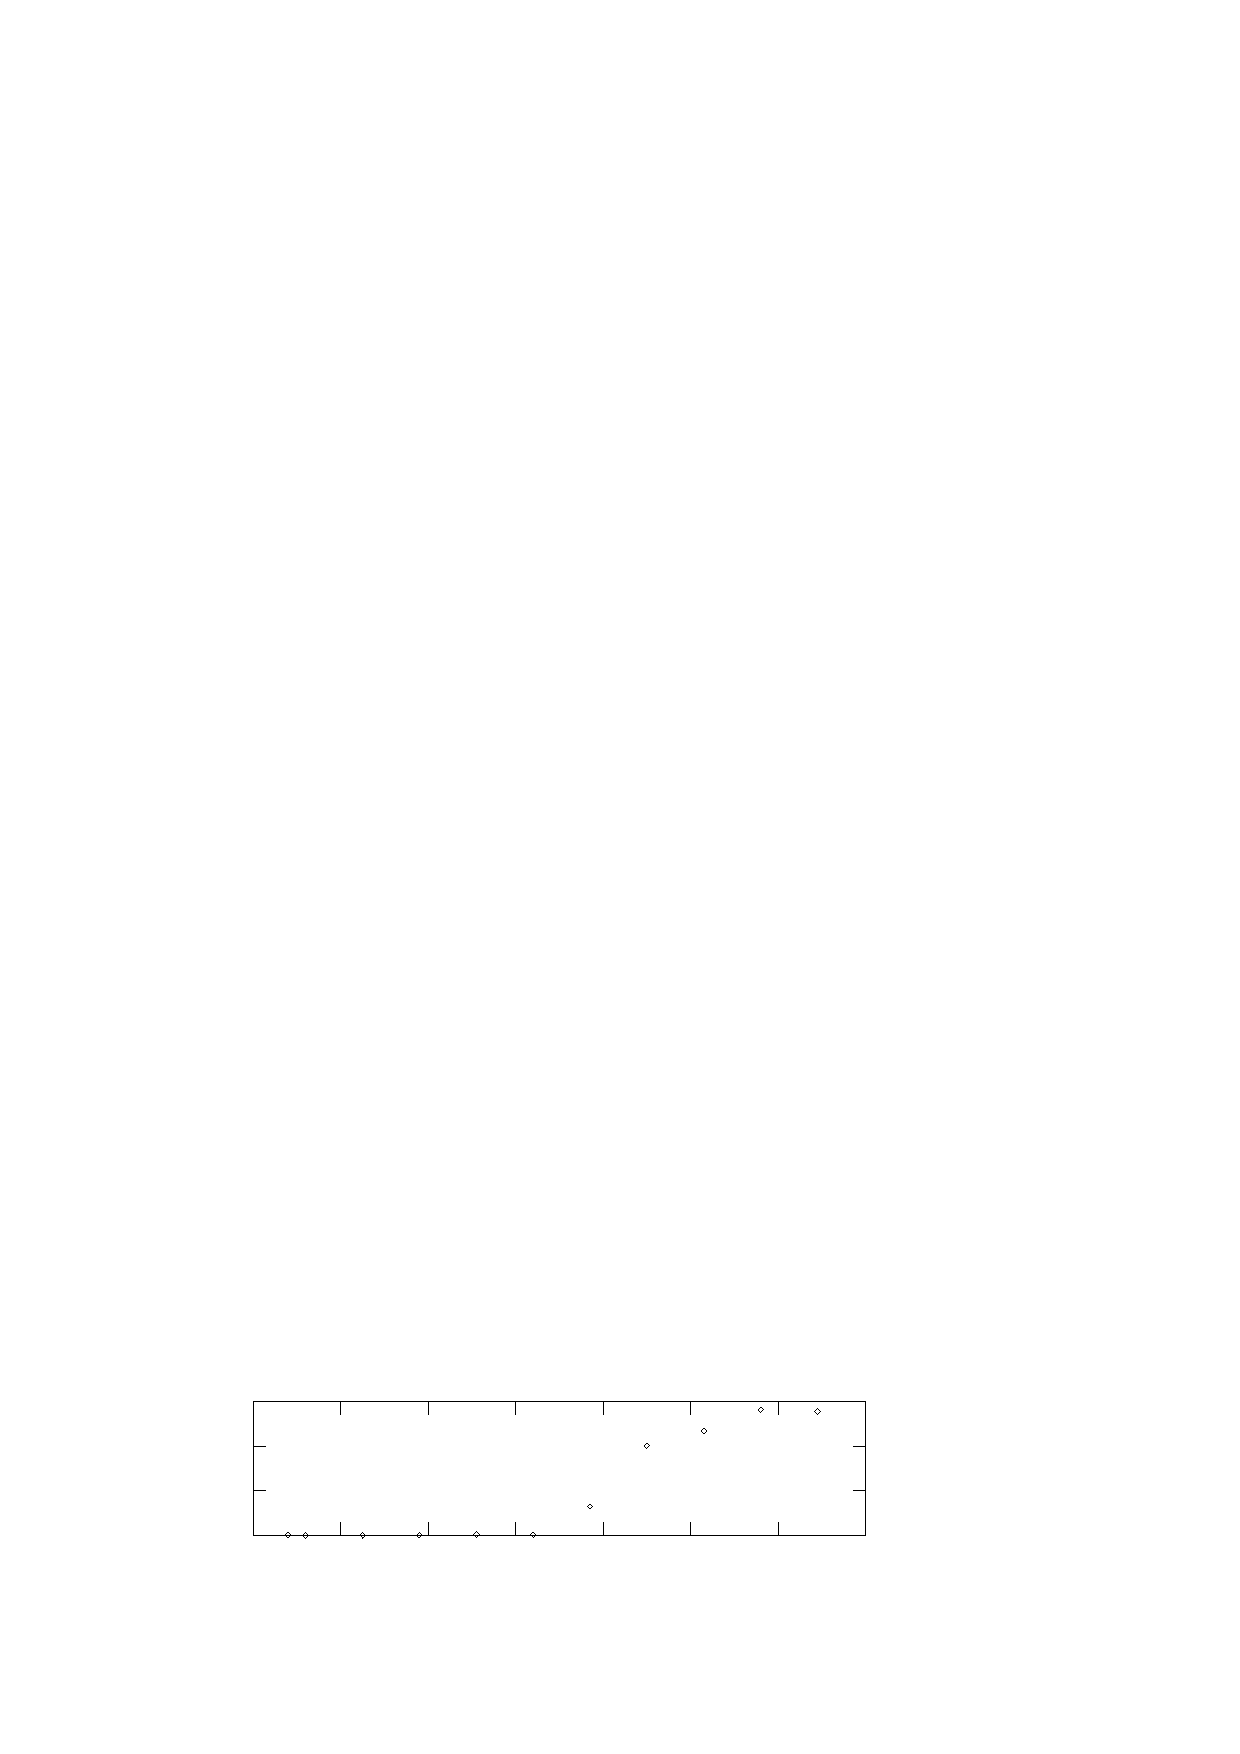
\includegraphics{Fo-equilibrium-amplitud-rounded-x}%
%\end{picture}%
%\begingroup
%\setlength{\unitlength}{0.0200bp}%
%\begin{picture}(18000,5400)(0,0)%
%\put(2200,1650){\makebox(0,0)[r]{\strut{}0.00}}%
%\put(2200,2717){\makebox(0,0)[r]{\strut{}0.50}}%
%\put(2200,3783){\makebox(0,0)[r]{\strut{}1.00}}%
%\put(2200,4850){\makebox(0,0)[r]{\strut{}1.50}}%
%\put(2475,1100){\makebox(0,0){\strut{}0.000}}%
%\put(4575,1100){\makebox(0,0){\strut{}0.001}}%
%\put(6675,1100){\makebox(0,0){\strut{}0.002}}%
%\put(8775,1100){\makebox(0,0){\strut{}0.003}}%
%\put(10875,1100){\makebox(0,0){\strut{}0.004}}%
%\put(12975,1100){\makebox(0,0){\strut{}0.005}}%
%\put(15075,1100){\makebox(0,0){\strut{}0.006}}%
%\put(17175,1100){\makebox(0,0){\strut{}0.007}}%
%\put(550,3250){\rotatebox{90}{\makebox(0,0){\strut{}$\sigma_x^\ast$}}}%
%\put(9825,275){\makebox(0,0){\strut{}$P_o^\ast$}}%
%\put(600,1000){\rotatebox{0}{\makebox(0,0){\strut{}(c)}}}%
%\end{picture}%
%\endgroup
%\endinput

\caption{\label{fig:barrido-momento}
Posici'on vertical y desviaci'on est'andar en la direcci'on vertical 
como funci'on de la cantidad de movimiento agregado  $P_o^\ast$ con 
$\rho_p/\rho_f=50$ para la cavidad  (a) plana  y (b) redondeada. Para  
$P_o^\ast>4\times 10^{-3}$ la part'icula comienza a oscilar horizontalmente, como mostramos en (c).
Para la cavidad plana, el nodo de presi'on se mantiene constante en 1.6 y para la cavidad
redondeada, indicamos la posici'on del nodo de presi'on por la l'inea con puntos en (b). 
}
\end{figure}

En el siguiente conjunto de simulaciones num'ericas mantenemos constante la
relaci'on de densidades en  $\rho_p/\rho_f=50$  en presencia de un campo
gravitacional externo y variamos la cantidad de movimiento
agregada por la fuente ac'ustica $P_o^\ast$  para la cavidad plana y
la redondeada. Como en el conjunto de simulaciones num'ericas anteriores, medimos
la posici'on vertical en el estado estacionario y las desviaciones est'andar en ambas direcciones.
En las figuras~\ref{fig:barrido-momento} (a) y (b) mostramos estas mediciones 
como funci'on de la cantidad de movimiento para la cavidad plana y la redondeada, respectivamente. 
En (b) se muestra tambi'en la posici'on vertical del nodo de presi'on para la cavidad redondeada
por la l'inea con puntos. Conforme aumentamos la cantidad de movimiento agregada 
por la fuente ac'ustica, la part'icula es desplazada hacia el nodo de presi'on, 
como observamos de la figura~\ref{fig:barrido-momento} (a), para
la cavidad plana. Tambi'en, conforme aumenta la cantidad de movimiento agregada aumenta
el valor de $\sigma_y$.  Para la part'icula en la cavidad redondeada,  la posici'on estacionaria de la part'icula
se desplaza hacia el nodo de presi'on conforme aumentamos la cantidad de movimiento
agregada, pero para $P_{o}^\ast > 4\times 10^{-3}$ el desplazamiento ya no sigue la misma tendencia
y al mismo tiempo la part'icula comienza a oscilar  en el eje horizontal y el nodo de presi'on
sufre un desplazamiento en el eje vertical, como podemos
ver de la figuras~\ref{fig:barrido-momento} (b) y (c).
Es el movimiento horizontal de la part'icula, que no estaba presente en las
simulaciones anteriores, el que nos da una clave para entender el movimiento de la part'icula
para valores altos de $P_o^\ast$ junto con la posici'on de los nodos de presi'on, 
como veremos m'as adelante. Podemos decir que existe un valor para la cantidad de 
movimiento agregada por la fuente ac'ustica  $0.003 < P_{o_C}^\ast < 0.0035$ en el cual la part'icula
comienza a oscilar en el eje horizontal.



\begin{figure} 
%\put(600,2550){\rotatebox{90}{\makebox(0,0){\strut{}(a)}}}%
%%GNUPLOT: LaTeX picture with Postscript
%\begin{picture}(0,0)%
%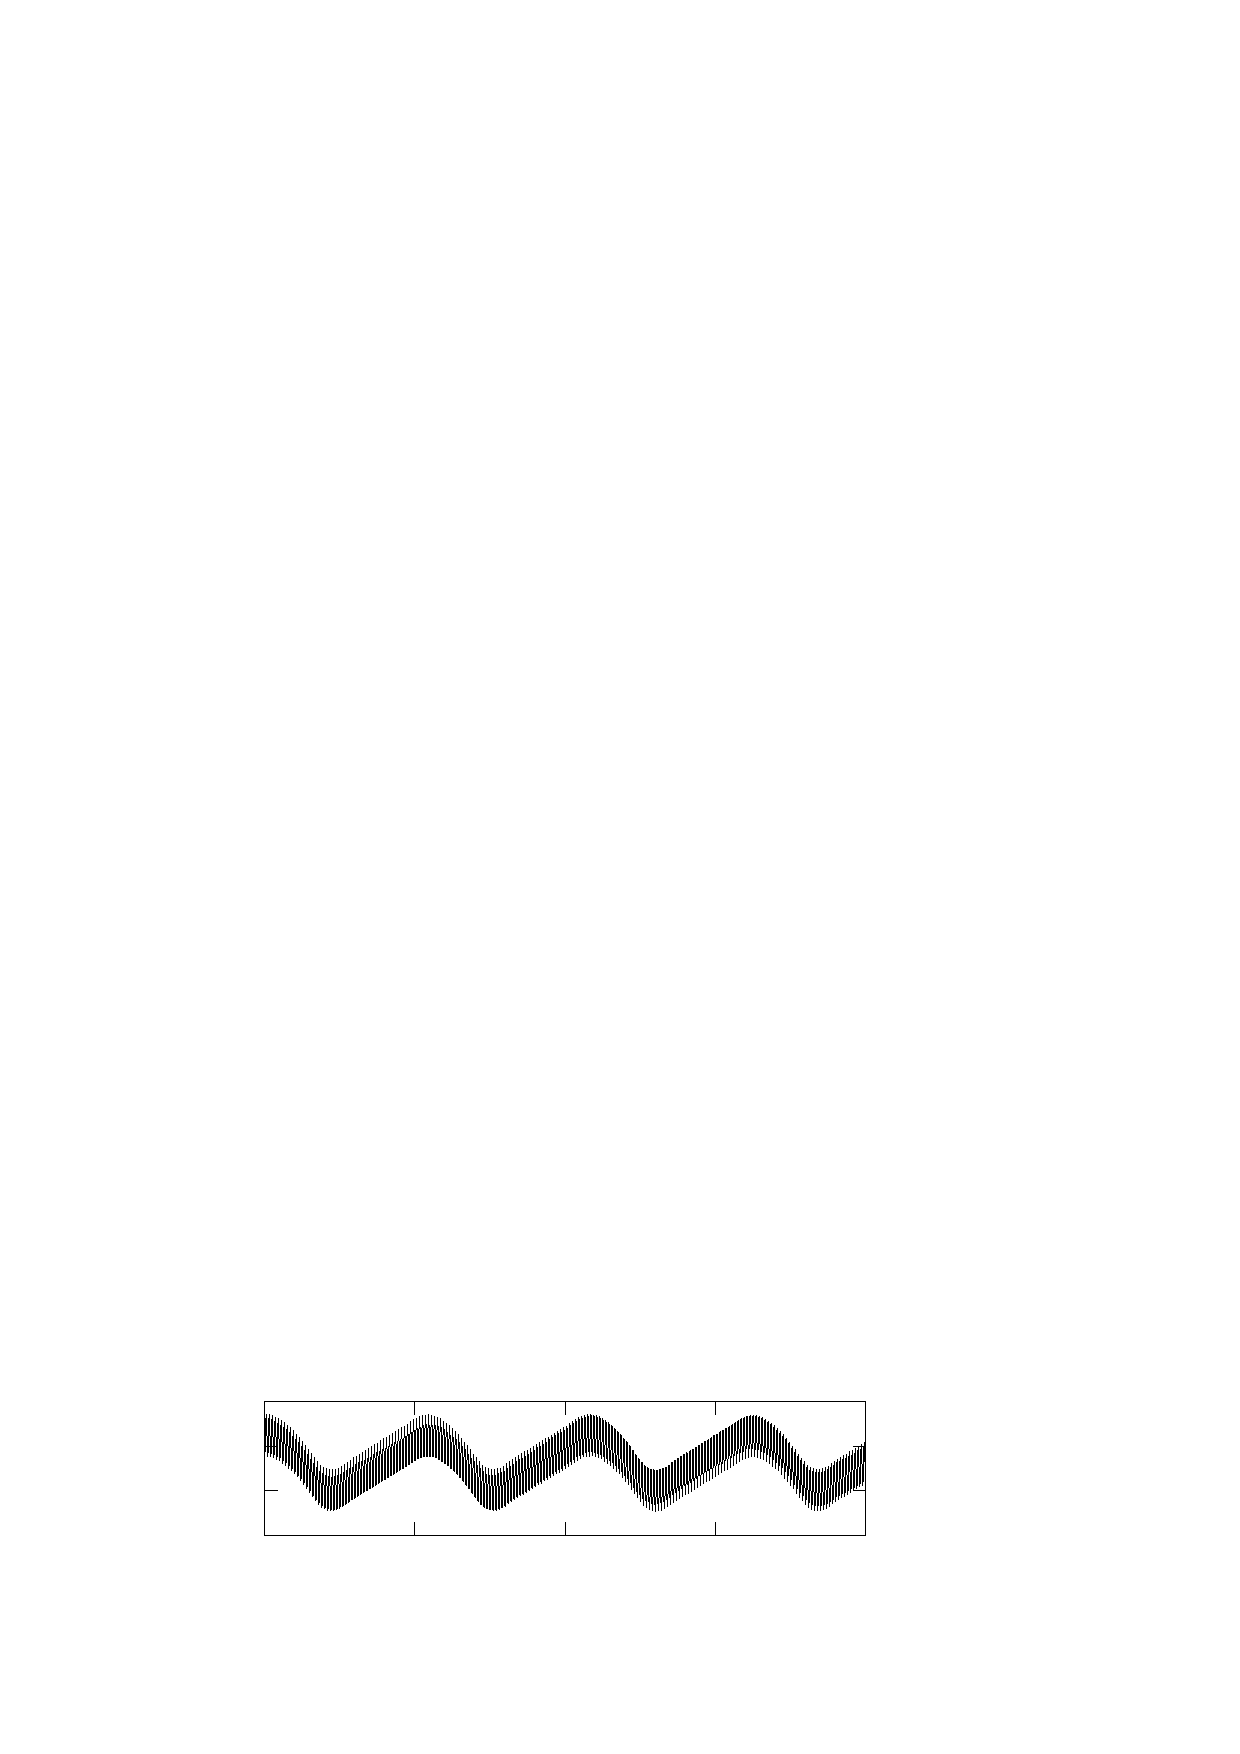
\includegraphics{flat-rho-30-Fo5_569e-02}%
%\end{picture}%
%\begingroup
%\setlength{\unitlength}{0.0200bp}%
%\begin{picture}(18000,5400)(0,0)%
%\put(2475,1650){\makebox(0,0)[r]{\strut{}1.179}}%
%\put(2475,2717){\makebox(0,0)[r]{\strut{}1.188}}%
%\put(2475,3783){\makebox(0,0)[r]{\strut{}1.197}}%
%\put(2475,4850){\makebox(0,0)[r]{\strut{}1.206}}%
%\put(2750,1100){\makebox(0,0){\strut{} 1600}}%
%\put(6356,1100){\makebox(0,0){\strut{} 1650}}%
%\put(9963,1100){\makebox(0,0){\strut{} 1700}}%
%\put(13569,1100){\makebox(0,0){\strut{} 1750}}%
%\put(17175,1100){\makebox(0,0){\strut{} 1800}}%
%\put(550,3250){\rotatebox{90}{\makebox(0,0){\strut{}$y^\ast$}}}%
%\put(9962,275){\makebox(0,0){\strut{}$t^\ast$}}%
%\put(600,1000){\rotatebox{0}{\makebox(0,0){\strut{}(a)}}}%
%\end{picture}%
%\endgroup
%\endinput

%%GNUPLOT: LaTeX picture with Postscript
%\begin{picture}(0,0)%
%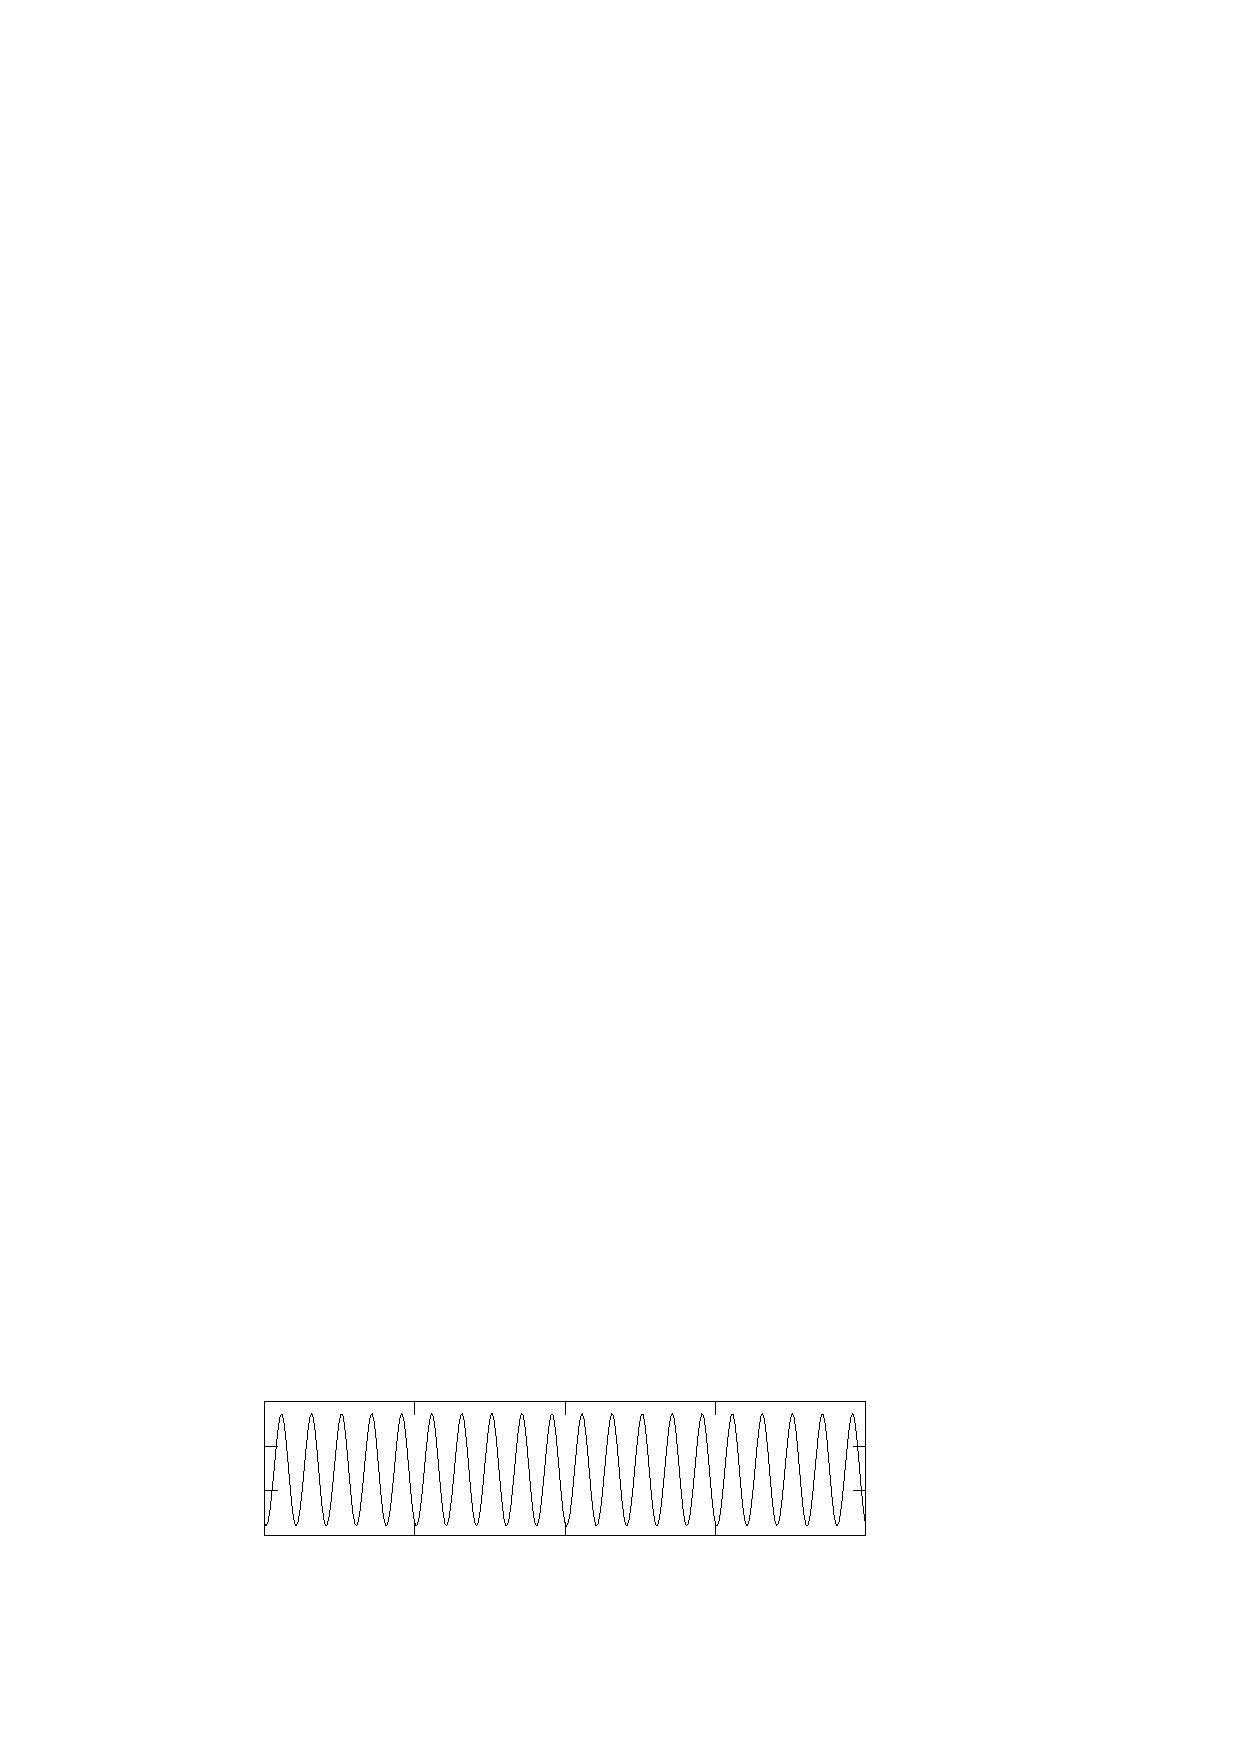
\includegraphics{flat-rho-30-Fo7_821e-02}%
%\end{picture}%
%\begingroup
%\setlength{\unitlength}{0.0200bp}%
%\begin{picture}(18000,5400)(0,0)%
%\put(2475,1650){\makebox(0,0)[r]{\strut{}1.400}}%
%\put(2475,2717){\makebox(0,0)[r]{\strut{}1.405}}%
%\put(2475,3783){\makebox(0,0)[r]{\strut{}1.410}}%
%\put(2475,4850){\makebox(0,0)[r]{\strut{}1.415}}%
%\put(2750,1100){\makebox(0,0){\strut{} 1000}}%
%\put(6356,1100){\makebox(0,0){\strut{} 1005}}%
%\put(9963,1100){\makebox(0,0){\strut{} 1010}}%
%\put(13569,1100){\makebox(0,0){\strut{} 1015}}%
%\put(17175,1100){\makebox(0,0){\strut{} 1020}}%
%\put(550,3250){\rotatebox{90}{\makebox(0,0){\strut{}$y^\ast$}}}%
%\put(9962,275){\makebox(0,0){\strut{}$t^\ast$}}%
%\put(600,1000){\rotatebox{0}{\makebox(0,0){\strut{}(b)}}}%
%\end{picture}%
%\endgroup
%\endinput

%%GNUPLOT: LaTeX picture with Postscript
%\begin{picture}(0,0)%
%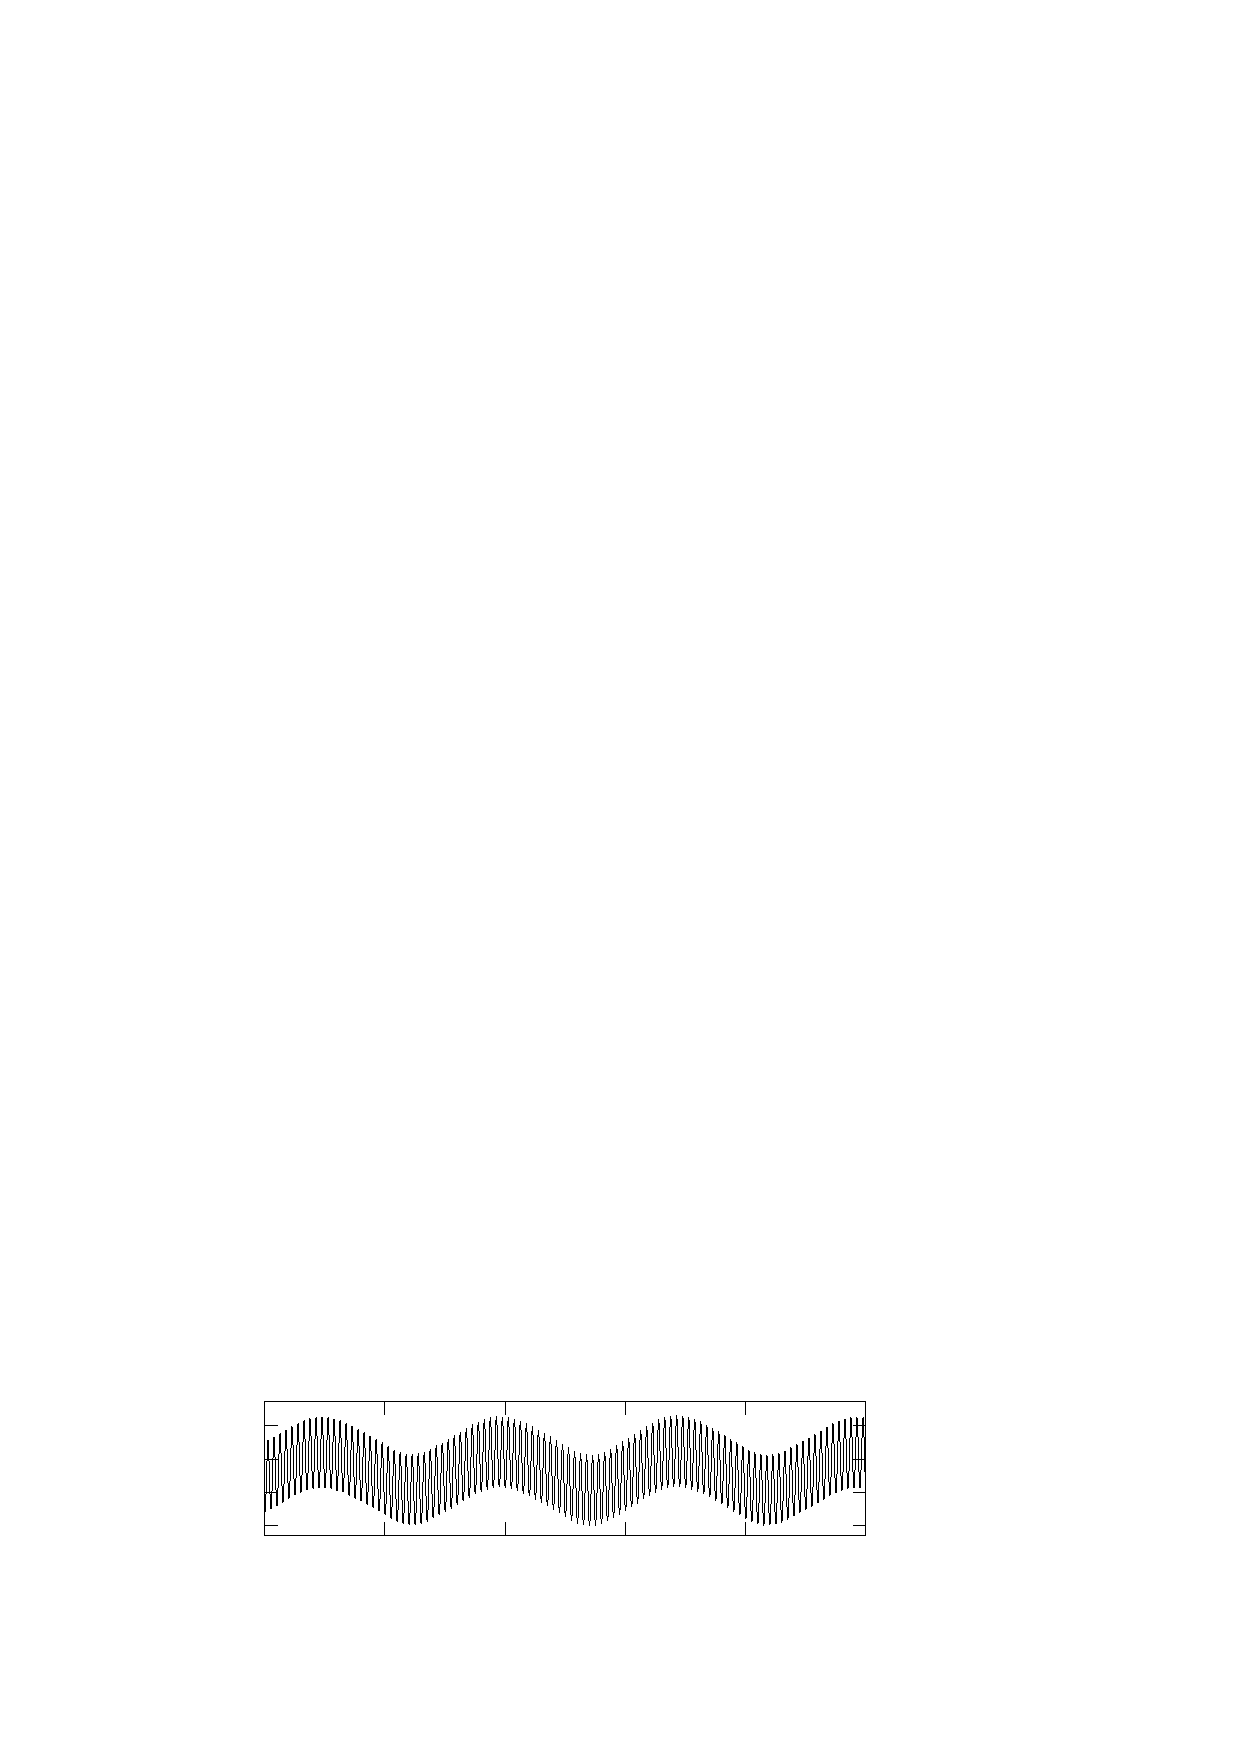
\includegraphics{flat-rho-30-Fo1_133e-01}%
%\end{picture}%
%\begingroup
%\setlength{\unitlength}{0.0200bp}%
%\begin{picture}(18000,5400)(0,0)%
%\put(2475,1879){\makebox(0,0)[r]{\strut{}1.488}}%
%\put(2475,2679){\makebox(0,0)[r]{\strut{}1.496}}%
%\put(2475,3479){\makebox(0,0)[r]{\strut{}1.505}}%
%\put(2475,4279){\makebox(0,0)[r]{\strut{}1.514}}%
%\put(2750,1100){\makebox(0,0){\strut{} 600}}%
%\put(5635,1100){\makebox(0,0){\strut{} 620}}%
%\put(8520,1100){\makebox(0,0){\strut{} 640}}%
%\put(11405,1100){\makebox(0,0){\strut{} 660}}%
%\put(14290,1100){\makebox(0,0){\strut{} 680}}%
%\put(17175,1100){\makebox(0,0){\strut{} 700}}%
%\put(550,3250){\rotatebox{90}{\makebox(0,0){\strut{}$y^\ast$}}}%
%\put(9962,275){\makebox(0,0){\strut{}$t^\ast$}}%
%\put(600,1000){\rotatebox{0}{\makebox(0,0){\strut{}(c)}}}%
%\end{picture}%
%\endgroup
%\endinput

%%GNUPLOT: LaTeX picture with Postscript
\begin{picture}(0,0)%
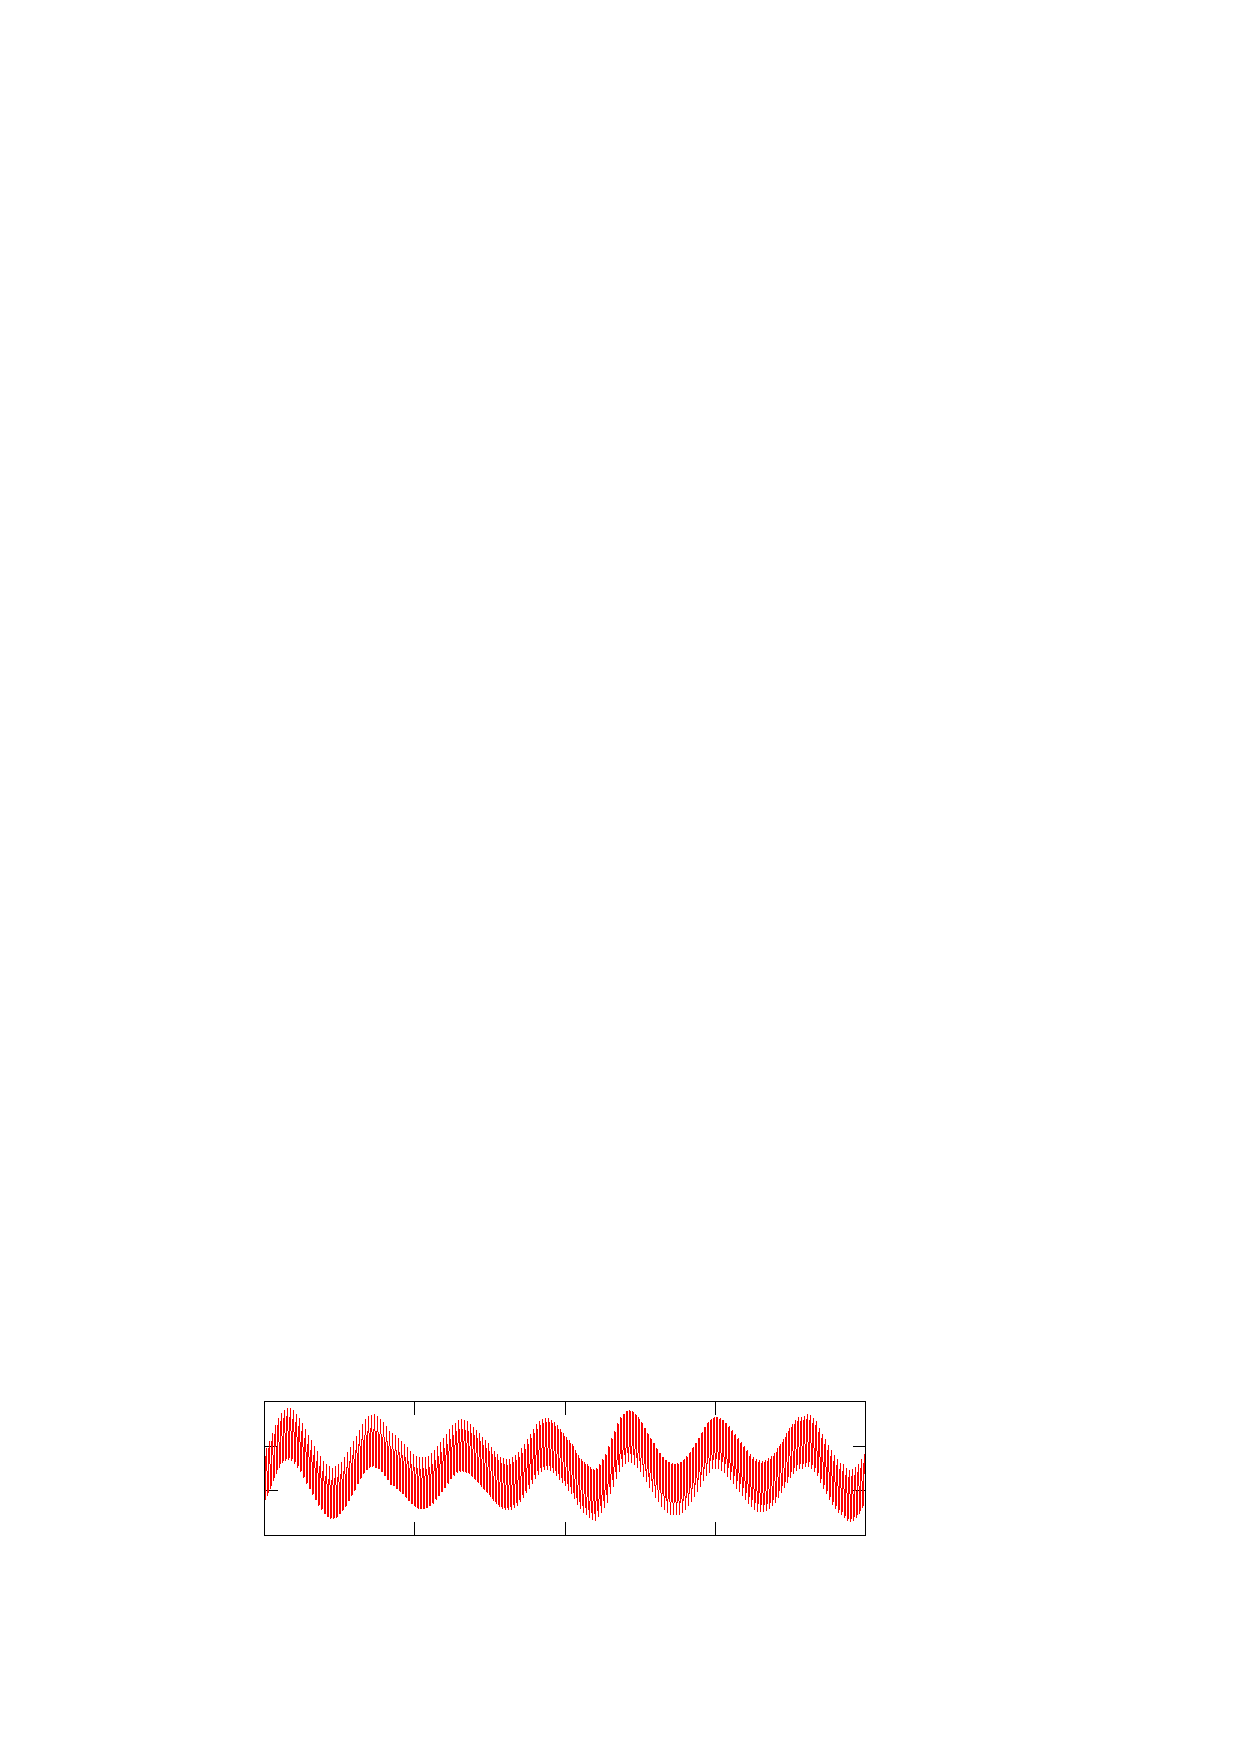
\includegraphics{flat-rho-30-Fo1_420e-01}%
\end{picture}%
\begingroup
\setlength{\unitlength}{0.0200bp}%
\begin{picture}(18000,5400)(0,0)%
\put(2475,1650){\makebox(0,0)[r]{\strut{}1.500}}%
\put(2475,2717){\makebox(0,0)[r]{\strut{}1.520}}%
\put(2475,3783){\makebox(0,0)[r]{\strut{}1.540}}%
\put(2475,4850){\makebox(0,0)[r]{\strut{}1.560}}%
\put(2750,1100){\makebox(0,0){\strut{} 1200}}%
\put(6356,1100){\makebox(0,0){\strut{} 1250}}%
\put(9963,1100){\makebox(0,0){\strut{} 1300}}%
\put(13569,1100){\makebox(0,0){\strut{} 1350}}%
\put(17175,1100){\makebox(0,0){\strut{} 1400}}%
\put(550,3250){\rotatebox{90}{\makebox(0,0){\strut{}$y^\ast$}}}%
\put(9962,275){\makebox(0,0){\strut{}$t^\ast$}}%
\put(600,2550){\rotatebox{90}{\makebox(0,0){\strut{}(d)}}}%
\end{picture}%
\endgroup
\endinput

%%GNUPLOT: LaTeX picture with Postscript
\begin{picture}(0,0)%
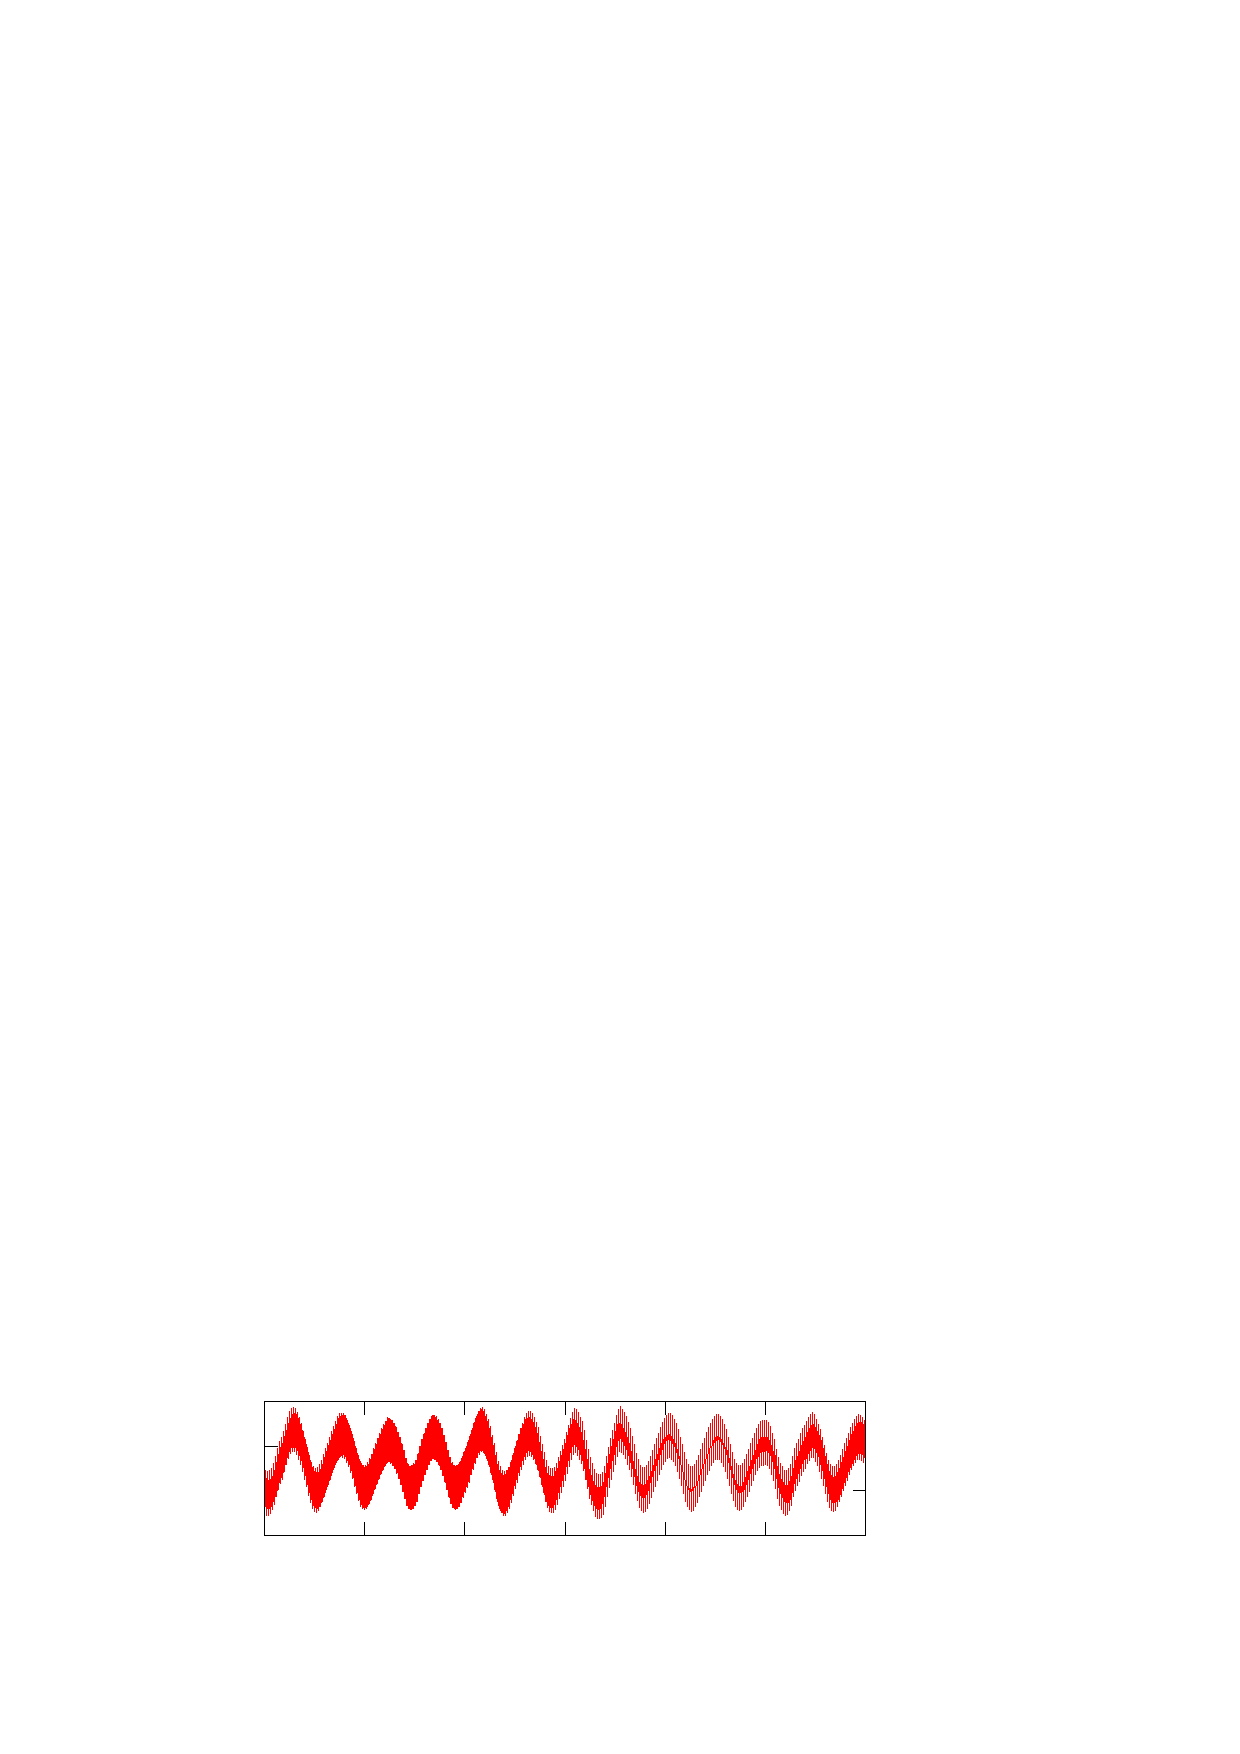
\includegraphics{flat-rho-30-Fo1_852e-01}%
\end{picture}%
\begingroup
\setlength{\unitlength}{0.0200bp}%
\begin{picture}(18000,5400)(0,0)%
\put(2475,1650){\makebox(0,0)[r]{\strut{}1.500}}%
\put(2475,2717){\makebox(0,0)[r]{\strut{}1.530}}%
\put(2475,3783){\makebox(0,0)[r]{\strut{}1.560}}%
\put(2475,4850){\makebox(0,0)[r]{\strut{}1.590}}%
\put(2750,1100){\makebox(0,0){\strut{} 1000}}%
\put(5154,1100){\makebox(0,0){\strut{} 1050}}%
\put(7558,1100){\makebox(0,0){\strut{} 1100}}%
\put(9963,1100){\makebox(0,0){\strut{} 1150}}%
\put(12367,1100){\makebox(0,0){\strut{} 1200}}%
\put(14771,1100){\makebox(0,0){\strut{} 1250}}%
\put(17175,1100){\makebox(0,0){\strut{} 1300}}%
\put(550,3250){\rotatebox{90}{\makebox(0,0){\strut{}$y^\ast$}}}%
\put(9962,275){\makebox(0,0){\strut{}$t^\ast$}}%
\put(600,2550){\rotatebox{90}{\makebox(0,0){\strut{}(e)}}}%
\end{picture}%
\endgroup
\endinput

\caption{\label{fig:paths-rho-30-flat}
Posici'on vertical de la part'icula s'olida $\rho_p/\rho_f=50$ sobre el tiempo en la cavidad plana para
(a) $P_o^\ast = 4.45\times 10^{-3} $, (b) $P_o^\ast = 6.25\times 10^{-3}$ y (c) $P_o^\ast = 9.05\times 10^{-3}$.
%(d) $P_o^\ast = 1.135\times 10^{-2}$ y (e) $P_o^\ast = 1.48\times 10^{-2}$.
}
\end{figure}
\begin{figure} 
%\put(600,2550){\rotatebox{90}{\makebox(0,0){\strut{}(a)}}}%
%%GNUPLOT: LaTeX picture with Postscript
%\begin{picture}(0,0)%
%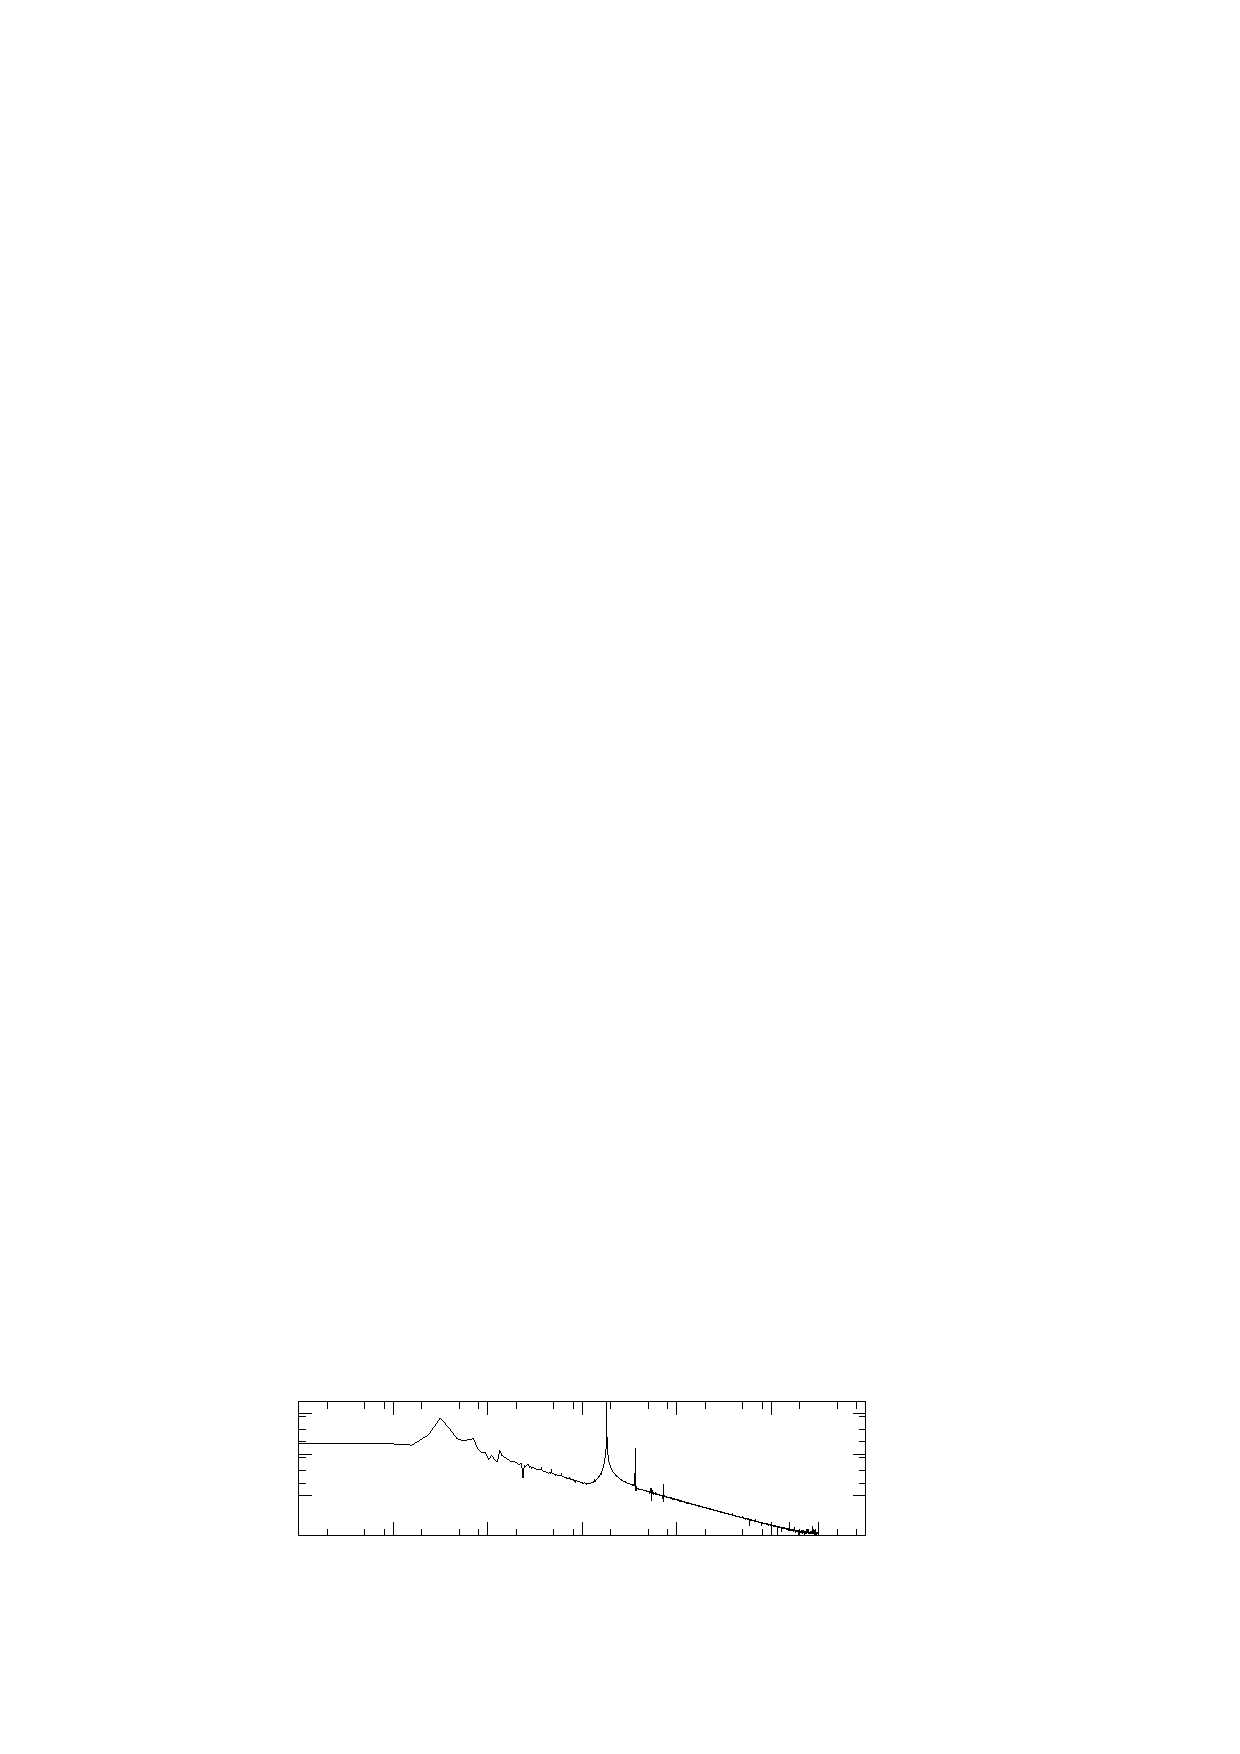
\includegraphics{flat-rho-30-Fo5_569e-02-spectrum}%
%\end{picture}%
%\begingroup
%\setlength{\unitlength}{0.0200bp}%
%\begin{picture}(18000,5400)(0,0)%
%\put(3300,2598){\makebox(0,0)[r]{\strut{}1.30e-13}}%
%\put(3300,3586){\makebox(0,0)[r]{\strut{}2.16e-10}}%
%\put(3300,4574){\makebox(0,0)[r]{\strut{}3.60e-07}}%
%\put(3575,1100){\makebox(0,0){\strut{} 1e-05}}%
%\put(5842,1100){\makebox(0,0){\strut{} 1e-04}}%
%\put(8108,1100){\makebox(0,0){\strut{} 0.001}}%
%\put(10375,1100){\makebox(0,0){\strut{} 0.01}}%
%\put(12642,1100){\makebox(0,0){\strut{} 0.1}}%
%\put(14908,1100){\makebox(0,0){\strut{} 1}}%
%\put(17175,1100){\makebox(0,0){\strut{} 10}}%
%\put(550,3250){\rotatebox{90}{\makebox(0,0){\strut{}$PSD$}}}%
%\put(10375,275){\makebox(0,0){\strut{}$\omega$}}%
%\put(600,1000){\makebox(0,0){\strut{}(a)}}%
%\end{picture}%
%\endgroup
%\endinput

%%GNUPLOT: LaTeX picture with Postscript
%\begin{picture}(0,0)%
%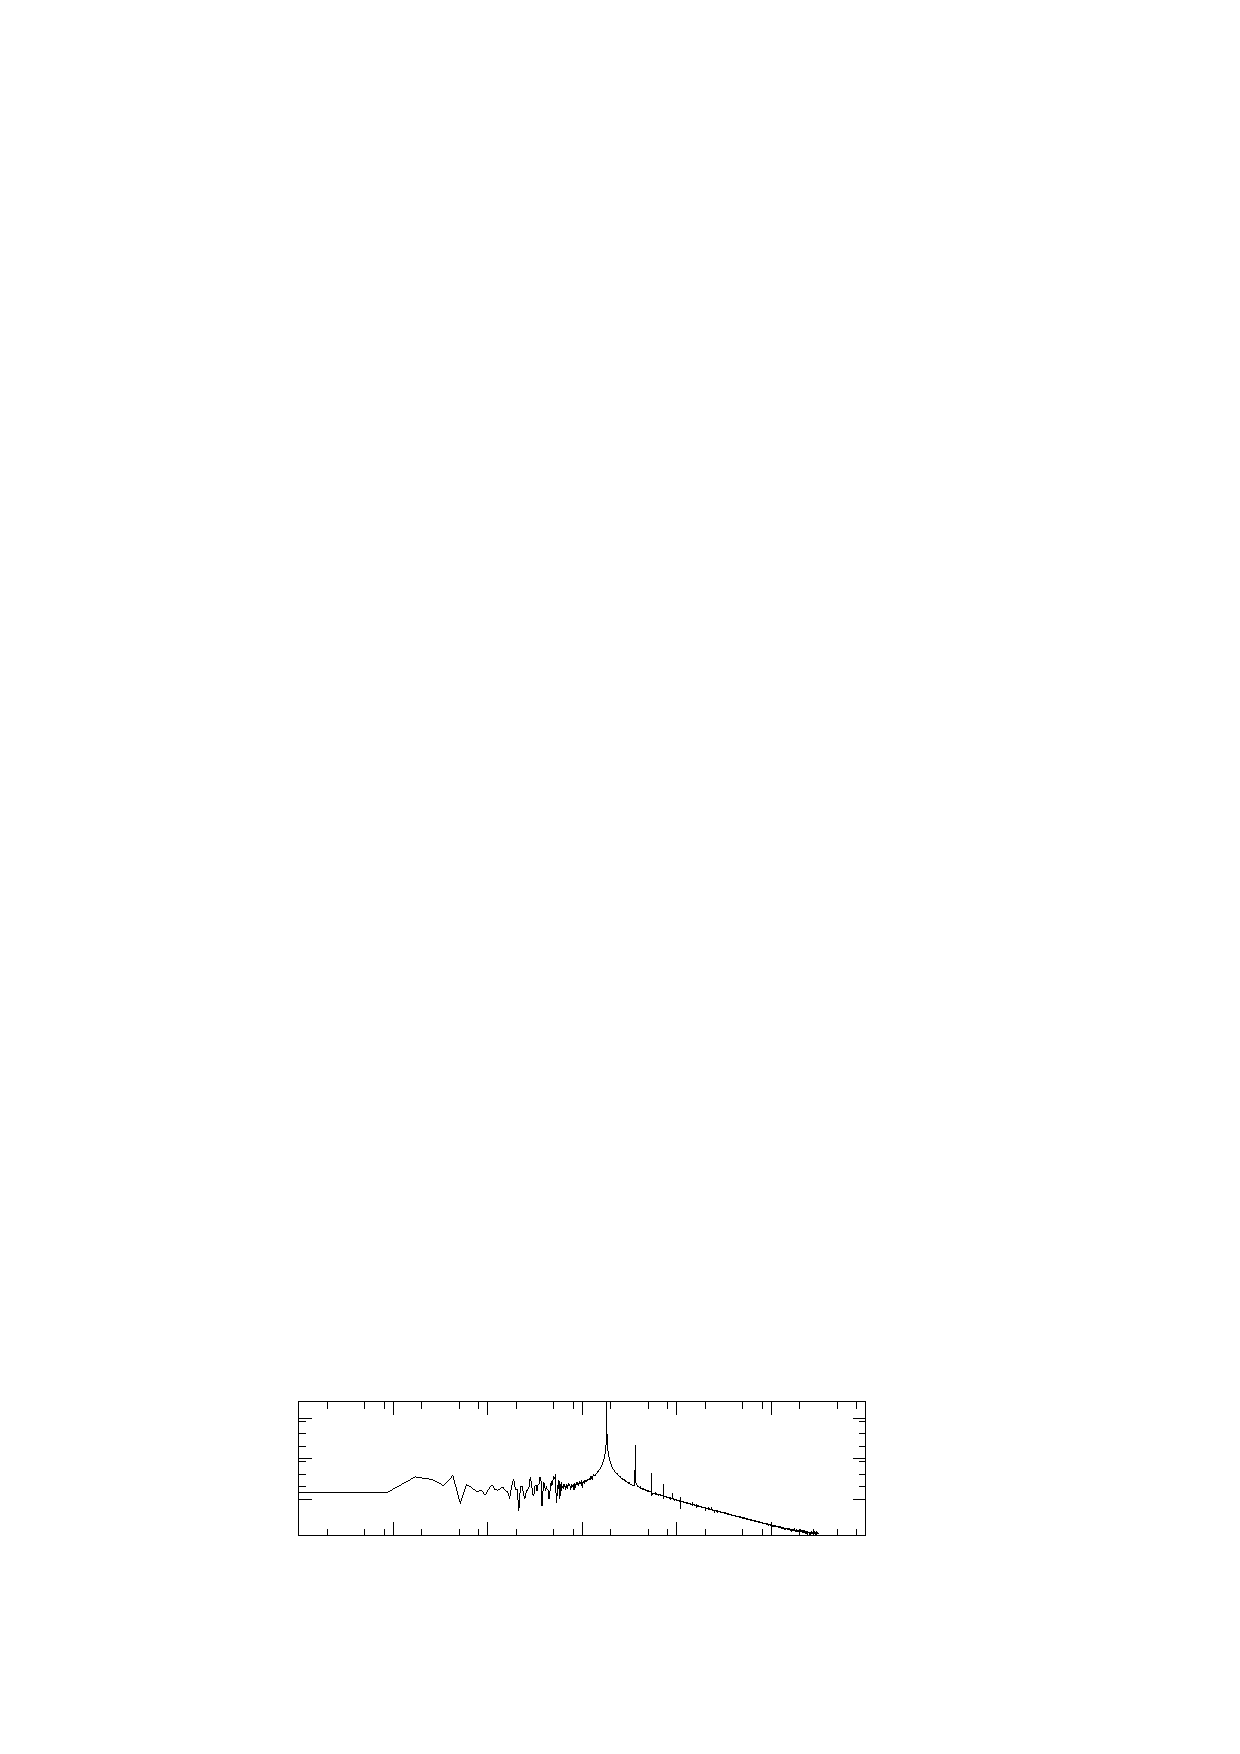
\includegraphics{flat-rho-30-Fo7_821e-02-spectrum}%
%\end{picture}%
%\begingroup
%\setlength{\unitlength}{0.0200bp}%
%\begin{picture}(18000,5400)(0,0)%
%\put(3300,2512){\makebox(0,0)[r]{\strut{}1.30e-13}}%
%\put(3300,3484){\makebox(0,0)[r]{\strut{}2.16e-10}}%
%\put(3300,4456){\makebox(0,0)[r]{\strut{}3.60e-07}}%
%\put(3575,1100){\makebox(0,0){\strut{} 1e-05}}%
%\put(5842,1100){\makebox(0,0){\strut{} 1e-04}}%
%\put(8108,1100){\makebox(0,0){\strut{} 0.001}}%
%\put(10375,1100){\makebox(0,0){\strut{} 0.01}}%
%\put(12642,1100){\makebox(0,0){\strut{} 0.1}}%
%\put(14908,1100){\makebox(0,0){\strut{} 1}}%
%\put(17175,1100){\makebox(0,0){\strut{} 10}}%
%\put(550,3250){\rotatebox{90}{\makebox(0,0){\strut{}$PSD$}}}%
%\put(10375,275){\makebox(0,0){\strut{}$\omega$}}%
%\put(600,1000){\rotatebox{0}{\makebox(0,0){\strut{}(b)}}}%
%\end{picture}%
%\endgroup
%\endinput

%%GNUPLOT: LaTeX picture with Postscript
%\begin{picture}(0,0)%
%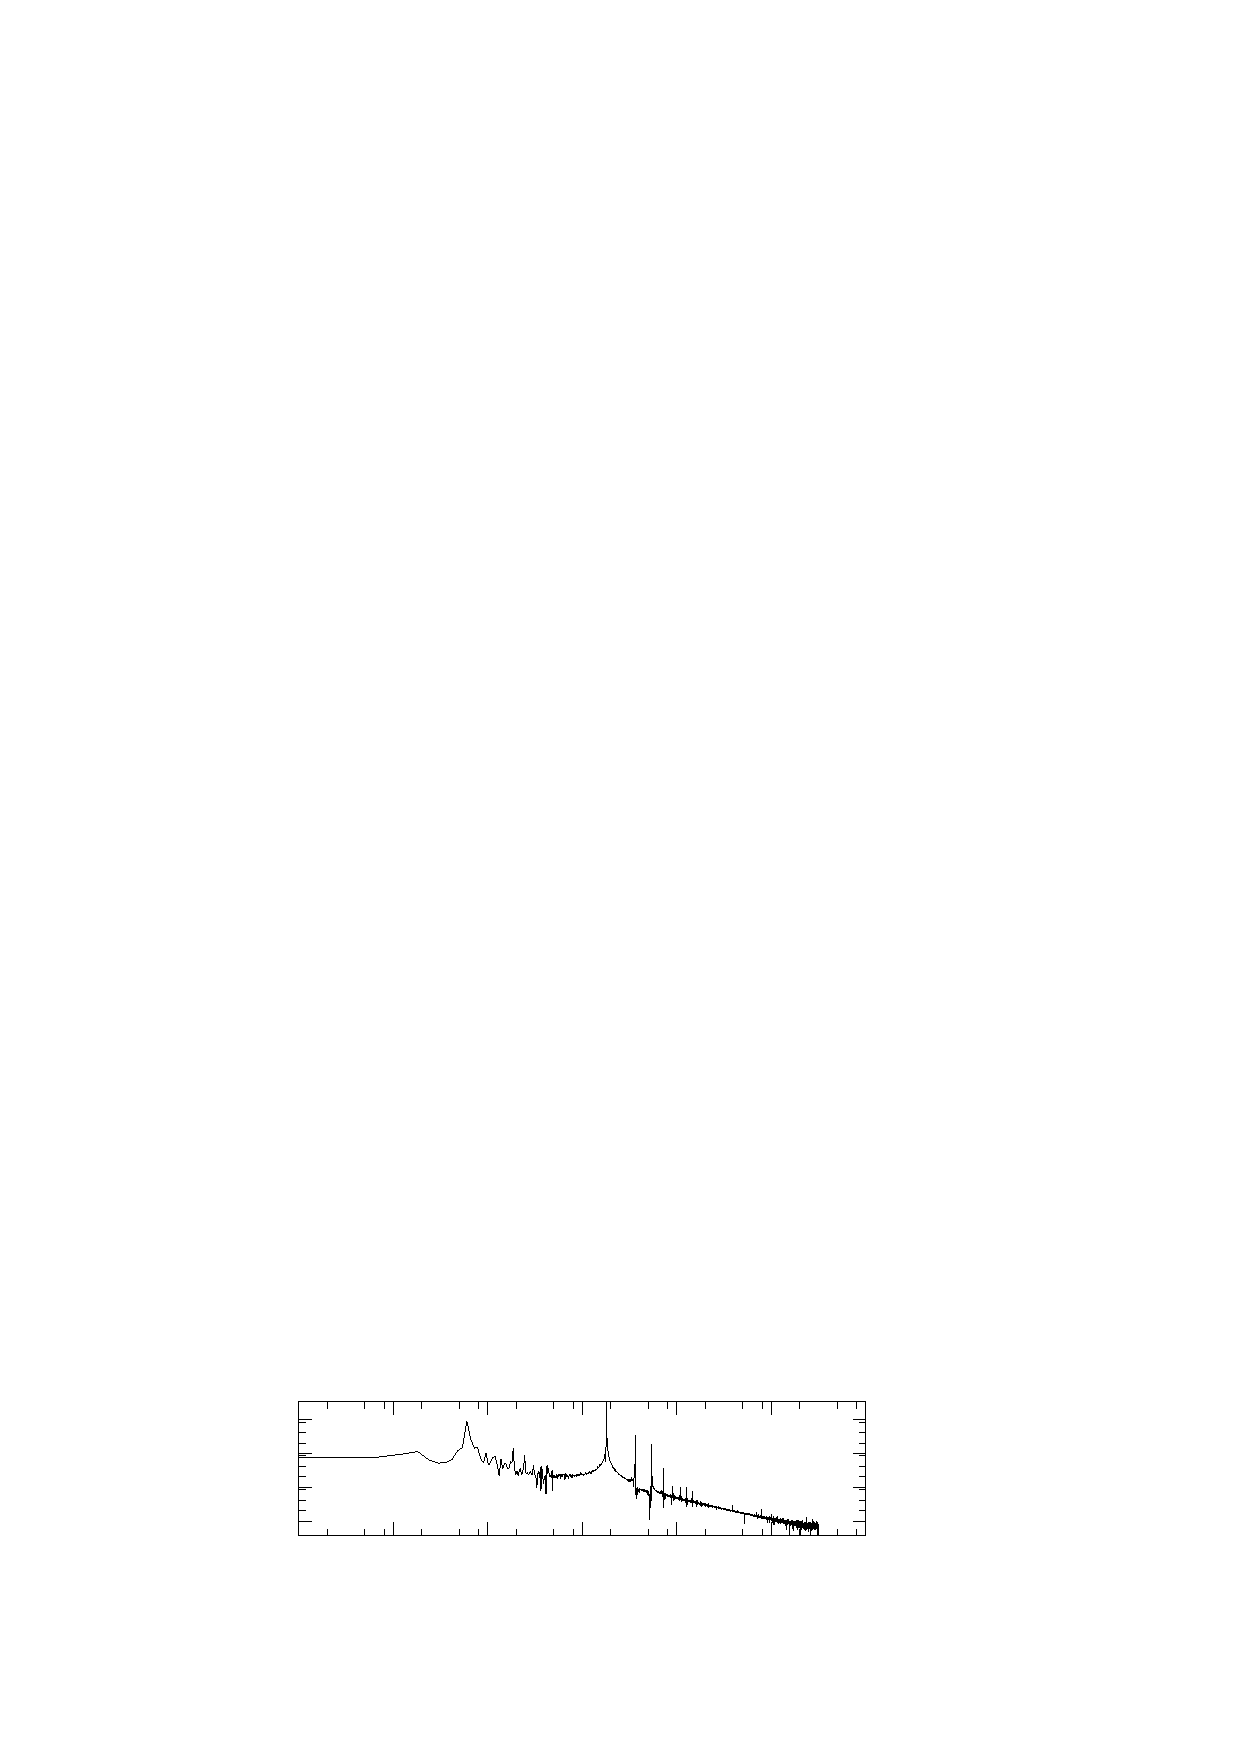
\includegraphics{flat-rho-30-Fo1_133e-01-spectrum}%
%\end{picture}%
%\begingroup
%\setlength{\unitlength}{0.0200bp}%
%\begin{picture}(18000,5400)(0,0)%
%\put(3300,1987){\makebox(0,0)[r]{\strut{}7.78e-17}}%
%\put(3300,2798){\makebox(0,0)[r]{\strut{}1.30e-13}}%
%\put(3300,3609){\makebox(0,0)[r]{\strut{}2.16e-10}}%
%\put(3300,4420){\makebox(0,0)[r]{\strut{}3.60e-07}}%
%\put(3575,1100){\makebox(0,0){\strut{} 1e-05}}%
%\put(5842,1100){\makebox(0,0){\strut{} 1e-04}}%
%\put(8108,1100){\makebox(0,0){\strut{} 0.001}}%
%\put(10375,1100){\makebox(0,0){\strut{} 0.01}}%
%\put(12642,1100){\makebox(0,0){\strut{} 0.1}}%
%\put(14908,1100){\makebox(0,0){\strut{} 1}}%
%\put(17175,1100){\makebox(0,0){\strut{} 10}}%
%\put(550,3250){\rotatebox{90}{\makebox(0,0){\strut{}$PSD$}}}%
%\put(10375,275){\makebox(0,0){\strut{}$\omega$}}%
%\put(600,1000){\rotatebox{0}{\makebox(0,0){\strut{}(c)}}}%
%\end{picture}%
%\endgroup
%\endinput

%%GNUPLOT: LaTeX picture with Postscript
\begin{picture}(0,0)%
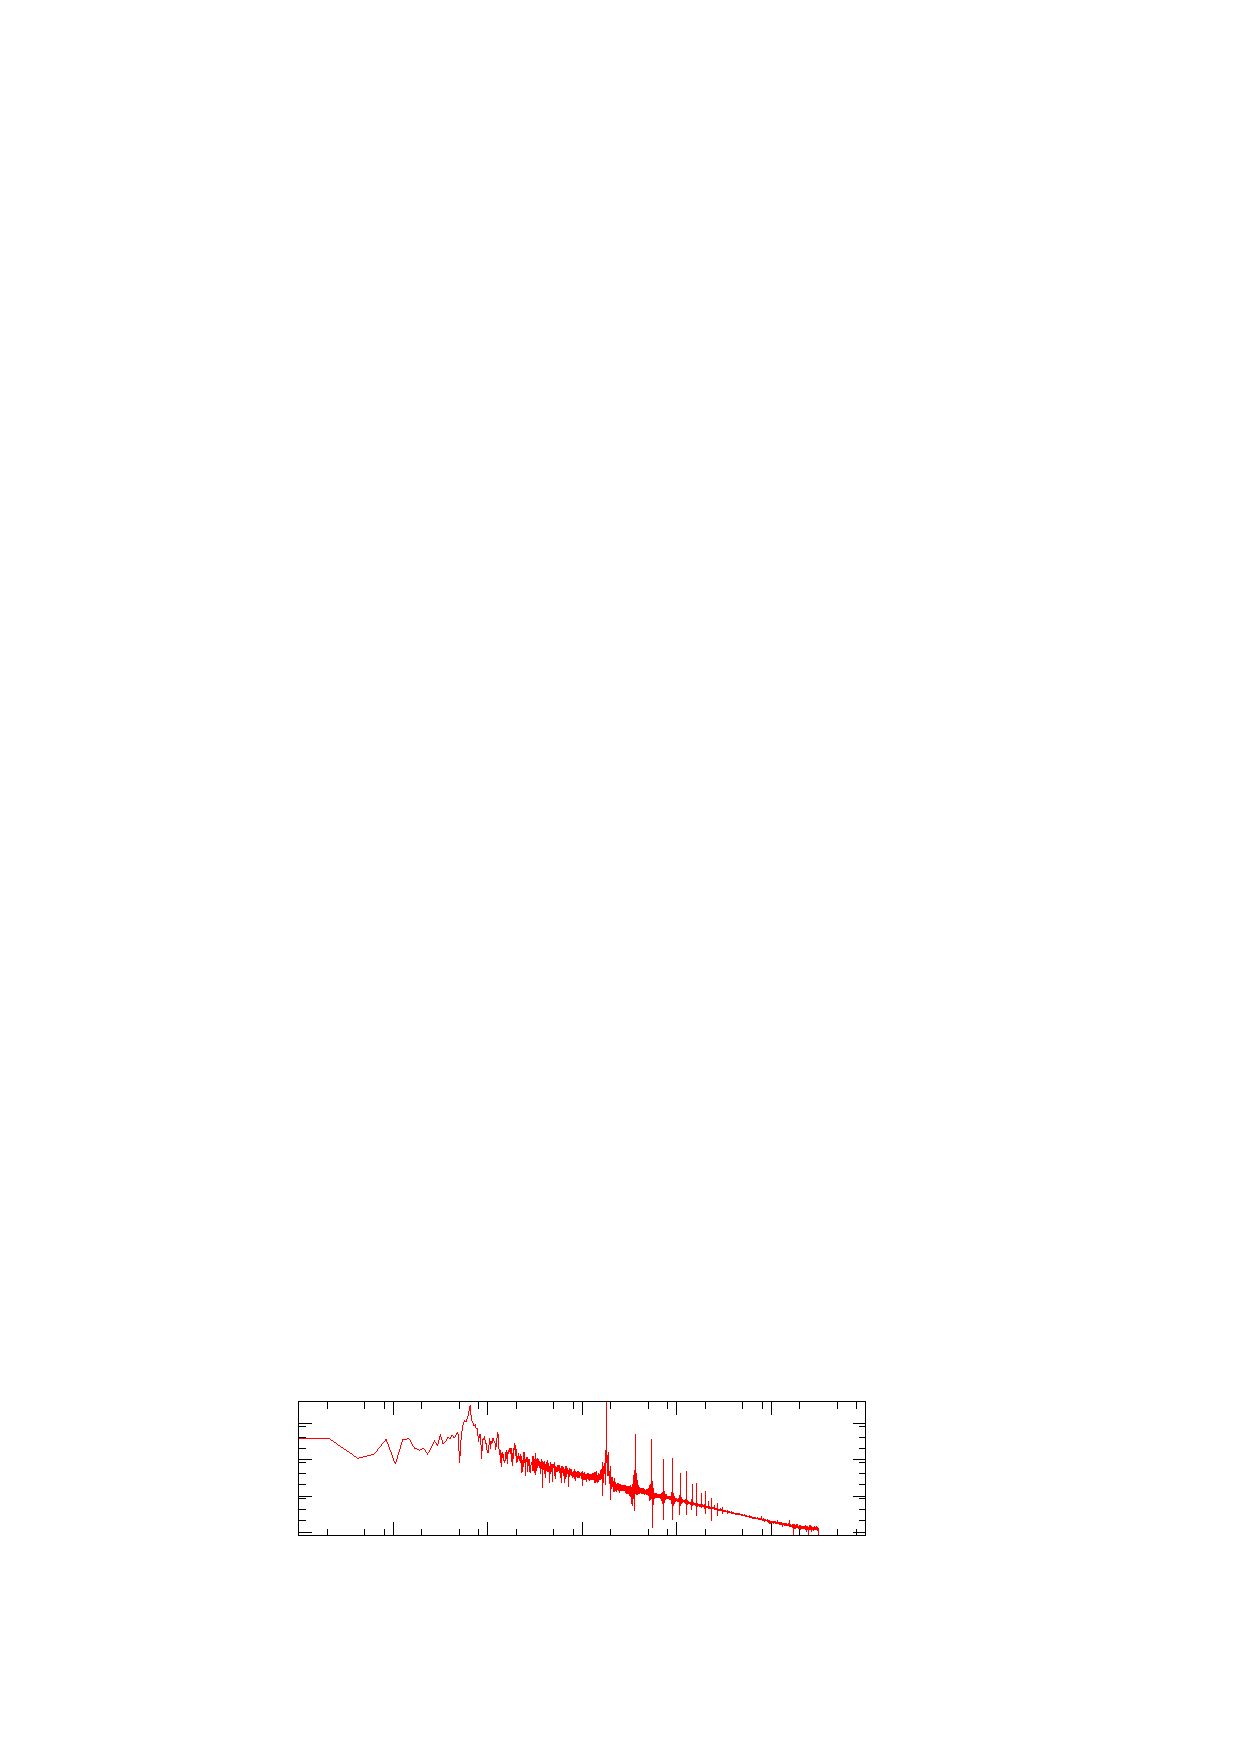
\includegraphics{flat-rho-30-Fo1_420e-01-spectrum}%
\end{picture}%
\begingroup
\setlength{\unitlength}{0.0200bp}%
\begin{picture}(18000,5400)(0,0)%
\put(3300,1724){\makebox(0,0)[r]{\strut{}7.78e-17}}%
\put(3300,2591){\makebox(0,0)[r]{\strut{}1.30e-13}}%
\put(3300,3457){\makebox(0,0)[r]{\strut{}2.16e-10}}%
\put(3300,4324){\makebox(0,0)[r]{\strut{}3.60e-07}}%
\put(3575,1100){\makebox(0,0){\strut{} 1e-05}}%
\put(5842,1100){\makebox(0,0){\strut{} 0.0001}}%
\put(8108,1100){\makebox(0,0){\strut{} 0.001}}%
\put(10375,1100){\makebox(0,0){\strut{} 0.01}}%
\put(12642,1100){\makebox(0,0){\strut{} 0.1}}%
\put(14908,1100){\makebox(0,0){\strut{} 1}}%
\put(17175,1100){\makebox(0,0){\strut{} 10}}%
\put(550,3250){\rotatebox{90}{\makebox(0,0){\strut{}$PSD$}}}%
\put(10375,275){\makebox(0,0){\strut{}$\omega$}}%
\put(600,2550){\rotatebox{90}{\makebox(0,0){\strut{}(d)}}}%
\end{picture}%
\endgroup
\endinput

%%GNUPLOT: LaTeX picture with Postscript
\begin{picture}(0,0)%
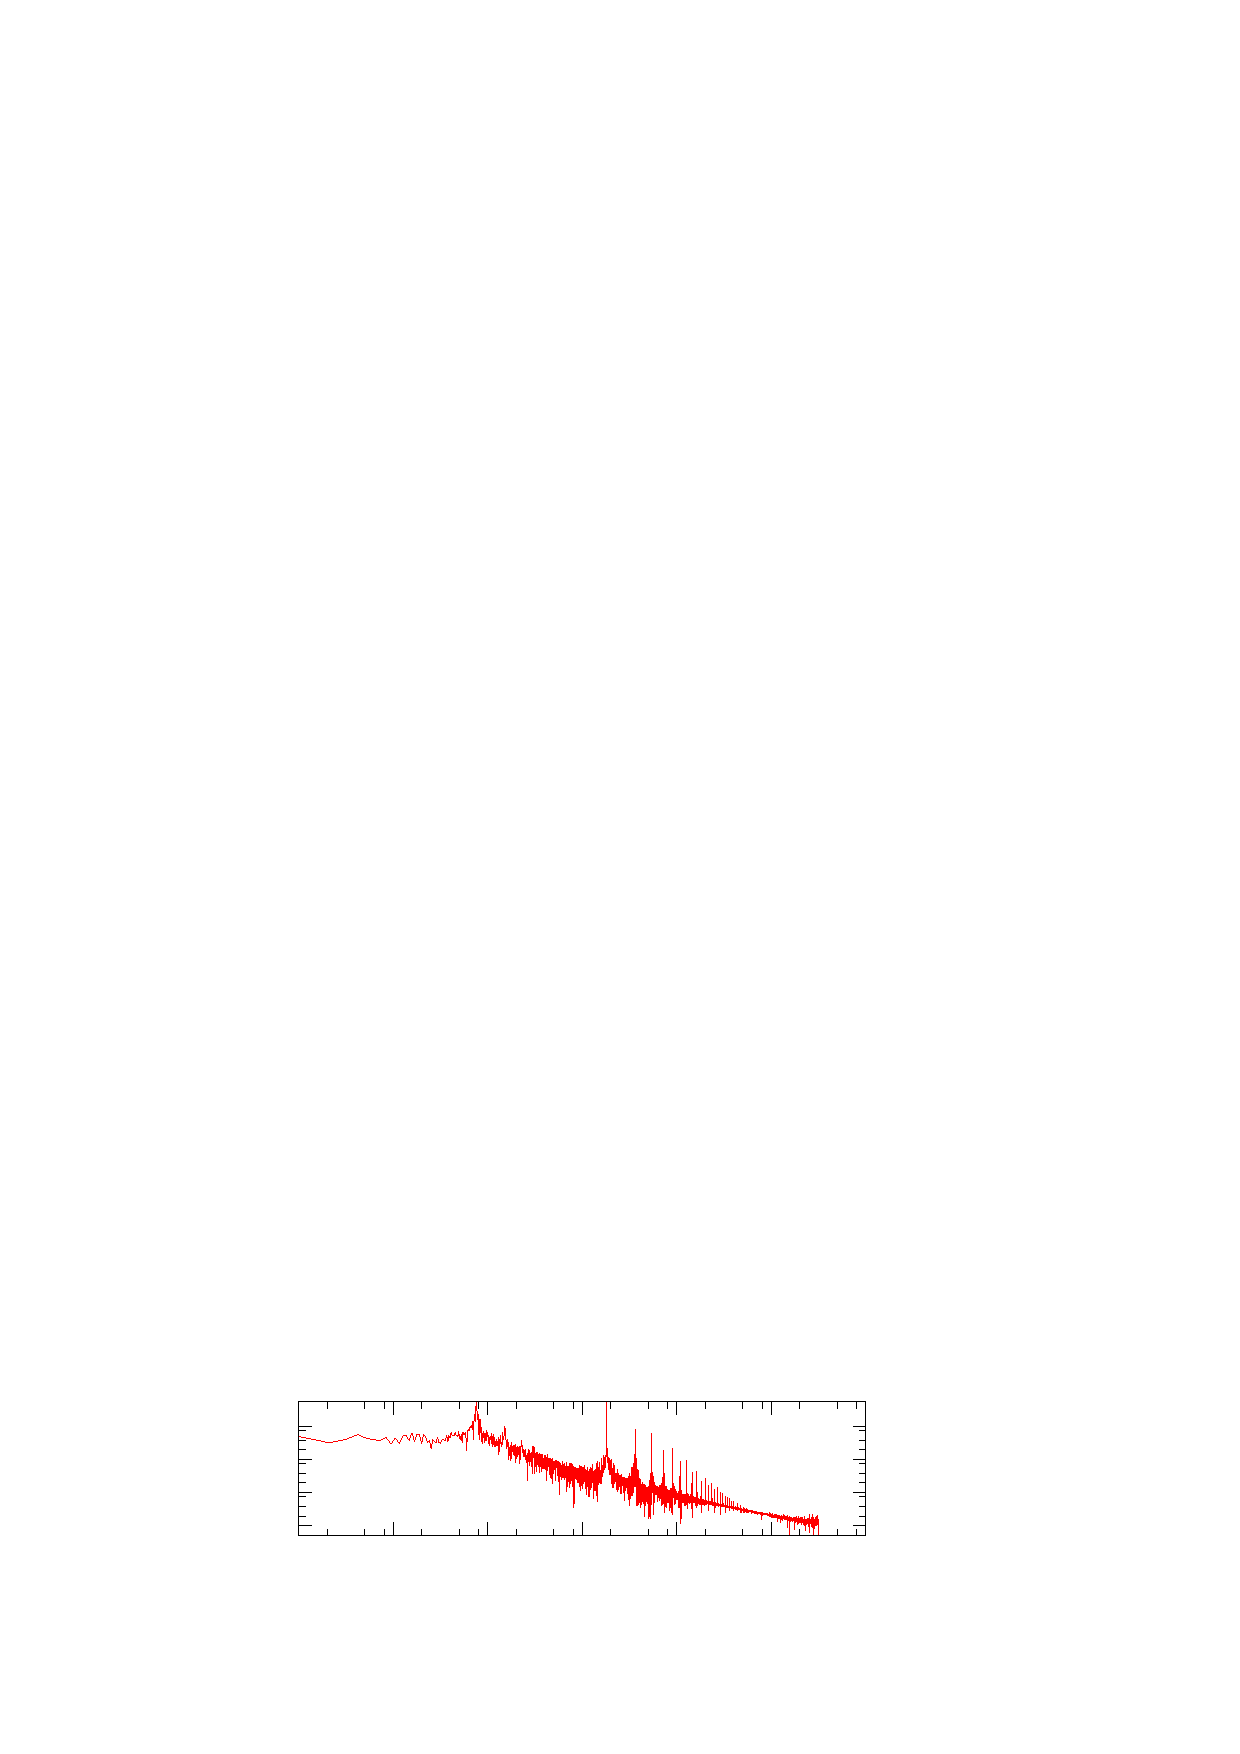
\includegraphics{flat-rho-30-Fo1_852e-01-spectrum}%
\end{picture}%
\begingroup
\setlength{\unitlength}{0.0200bp}%
\begin{picture}(18000,5400)(0,0)%
\put(3300,1878){\makebox(0,0)[r]{\strut{}1.02e-17}}%
\put(3300,2672){\makebox(0,0)[r]{\strut{}2.56e-14}}%
\put(3300,3466){\makebox(0,0)[r]{\strut{}6.40e-11}}%
\put(3300,4259){\makebox(0,0)[r]{\strut{}1.60e-07}}%
\put(3575,1100){\makebox(0,0){\strut{} 1e-05}}%
\put(5842,1100){\makebox(0,0){\strut{} 0.0001}}%
\put(8108,1100){\makebox(0,0){\strut{} 0.001}}%
\put(10375,1100){\makebox(0,0){\strut{} 0.01}}%
\put(12642,1100){\makebox(0,0){\strut{} 0.1}}%
\put(14908,1100){\makebox(0,0){\strut{} 1}}%
\put(17175,1100){\makebox(0,0){\strut{} 10}}%
\put(550,3250){\rotatebox{90}{\makebox(0,0){\strut{}$PSD$}}}%
\put(10375,275){\makebox(0,0){\strut{}$\omega$}}%
\put(600,2550){\rotatebox{90}{\makebox(0,0){\strut{}(e)}}}%
\end{picture}%
\endgroup
\endinput

\caption{\label{fig:paths-rho-30-flat-spectrum}
Espectro de potencia del movimiento vertical de la part'icula s'olida $\rho_p/\rho_f=50$ sobre el tiempo en la cavidad plana para
(a) $P_o^\ast = 4.45\times 10^{-3} $, (b) $P_o^\ast = 6.25\times 10^{-3}$ y (c) $P_o^\ast = 9.05\times 10^{-3}$. 
% (d) $P_o^\ast = 1.135\times 10^{-2}$ y (e) $P_o^\ast = 1.48\times 10^{-2}$.  
Los espectros de potencia corresponden  a las 
figuras~\ref{fig:paths-rho-30-flat} (a), (b) y (c).
}
\end{figure}

En las figuras~\ref{fig:paths-rho-30-flat} (a), (b) y (c) mostramos la posici'on vertical sobre el tiempo de la part'icula
s'olida en la cavidad plana para $P_o^\ast = 4.45\times 10^{-3} $, $P_o^\ast = 6.25\times 10^{-3}$ y $P_o^\ast = 9.05\times 10^{-3}$,
respectivamente. Al aumentar la cantidad de movimiento agregada, adem'as de aumentar la amplitud de la oscilaci'on
de la part'icula, tambi'en puede pasar por reg'imenes de oscilaci'on con una frecuencia o dos, como ha venido sucediendo
en las simulaciones num'ericas previas. Es curioso resaltar que para  $P_o^\ast = 6.25\times 10^{-3}$ el movimiento de 
la part'icula es m'as sencillo que para  $P_o^\ast = 4.45\times 10^{-3} $, que es un valor menor.
En las figuras~\ref{fig:paths-rho-30-flat-spectrum} (a), (b) y (c) mostramos los espectros
de potencia para las figuras mostradas anteriormente y observamos que  la presencia de arm'onicos de la frecuencia
de la fuente ac'ustica  ya es una constante.



\begin{figure} 
%\put(600,2550){\rotatebox{90}{\makebox(0,0){\strut{}(a)}}}%
%GNUPLOT: LaTeX picture with Postscript
\begin{picture}(0,0)%
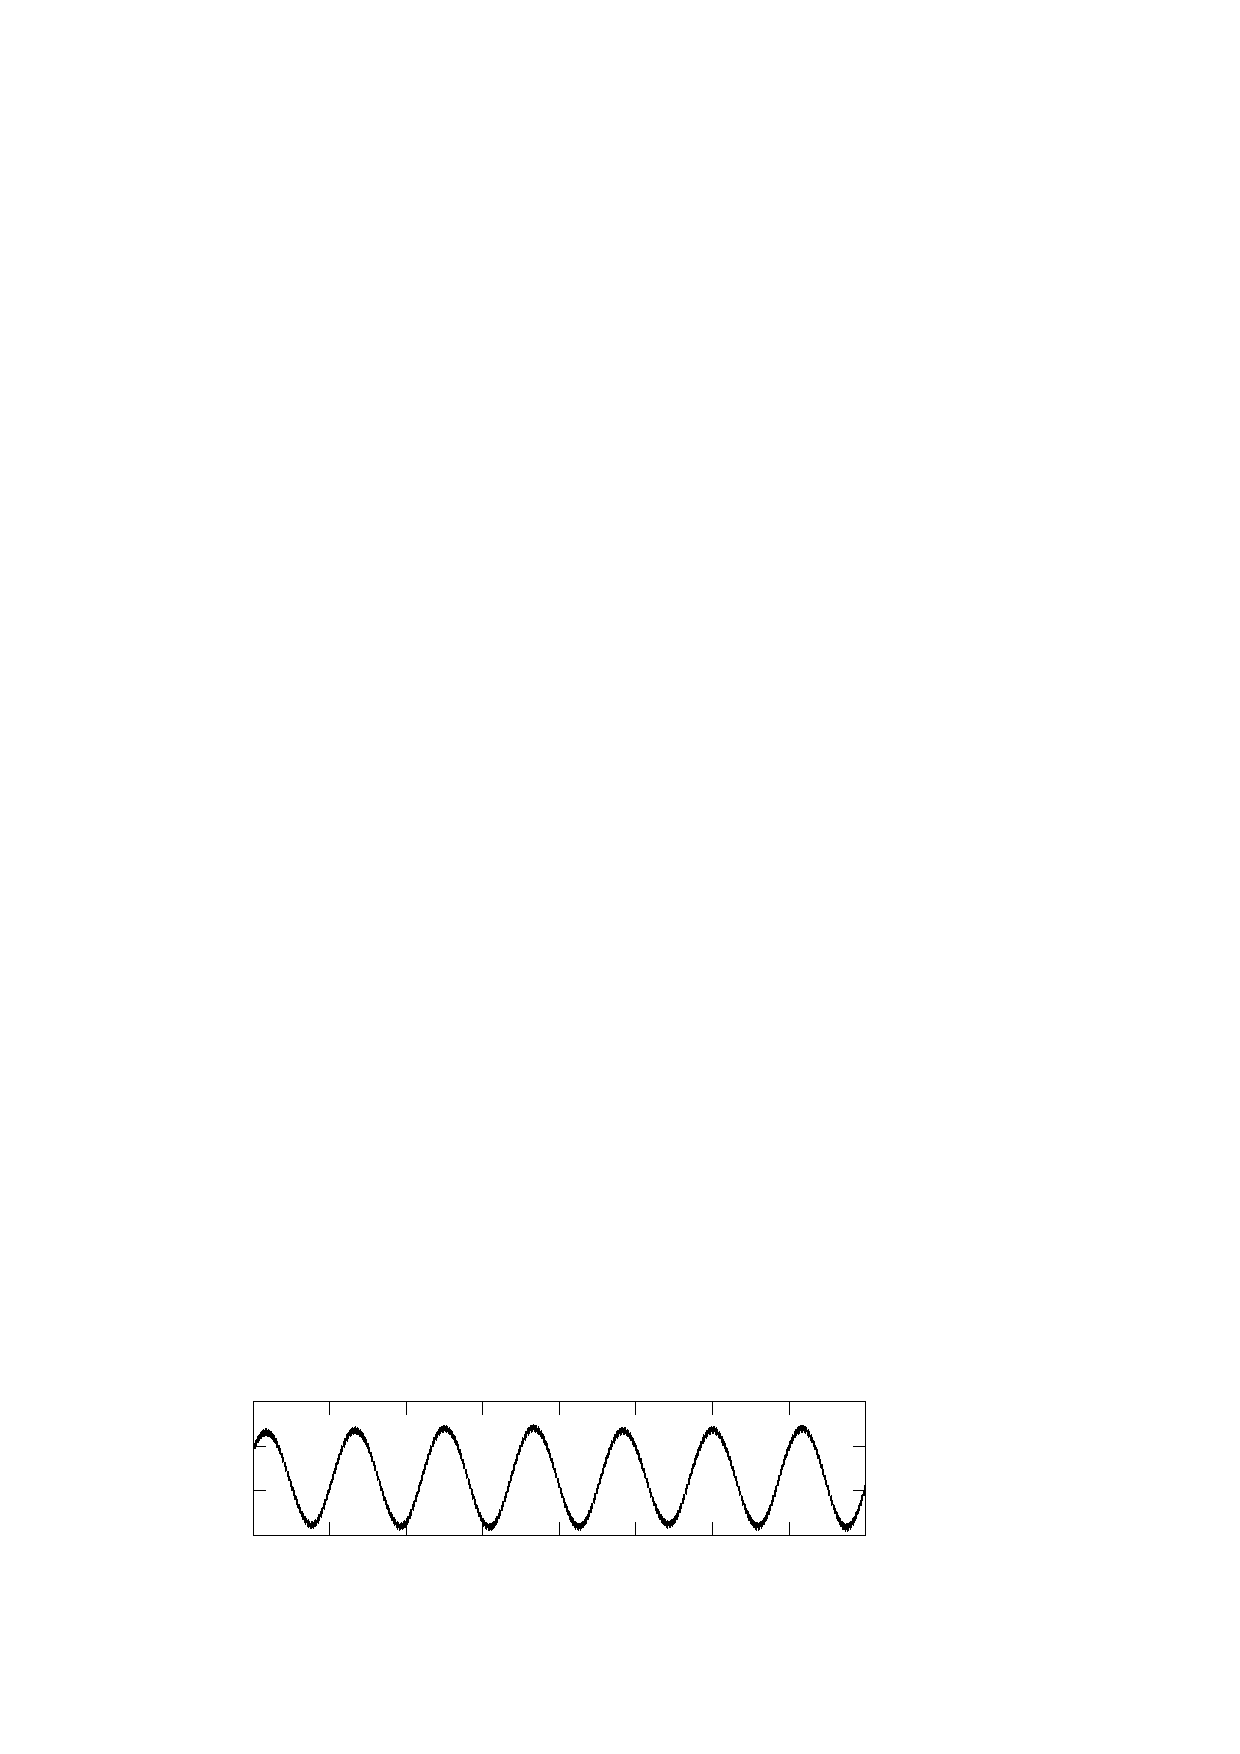
\includegraphics{rounded-rhop30-Fo7_508e-03}%
\end{picture}%
\begingroup
\setlength{\unitlength}{0.0200bp}%
\begin{picture}(18000,5400)(0,0)%
\put(2200,1650){\makebox(0,0)[r]{\strut{}1.14}}%
\put(2200,2717){\makebox(0,0)[r]{\strut{}1.20}}%
\put(2200,3783){\makebox(0,0)[r]{\strut{}1.26}}%
\put(2200,4850){\makebox(0,0)[r]{\strut{}1.32}}%
\put(2475,1100){\makebox(0,0){\strut{} 1800}}%
\put(6150,1100){\makebox(0,0){\strut{} 1850}}%
\put(9825,1100){\makebox(0,0){\strut{} 1900}}%
\put(13500,1100){\makebox(0,0){\strut{} 1950}}%
\put(17175,1100){\makebox(0,0){\strut{} 2000}}%
\put(550,3250){\rotatebox{90}{\makebox(0,0){\strut{}$y^\ast$}}}%
\put(9825,275){\makebox(0,0){\strut{}$t^\ast$}}%
\put(600,1000){\rotatebox{0}{\makebox(0,0){\strut{}(a)}}}%
\end{picture}%
\endgroup
\endinput

%%GNUPLOT: LaTeX picture with Postscript
%\begin{picture}(0,0)%
%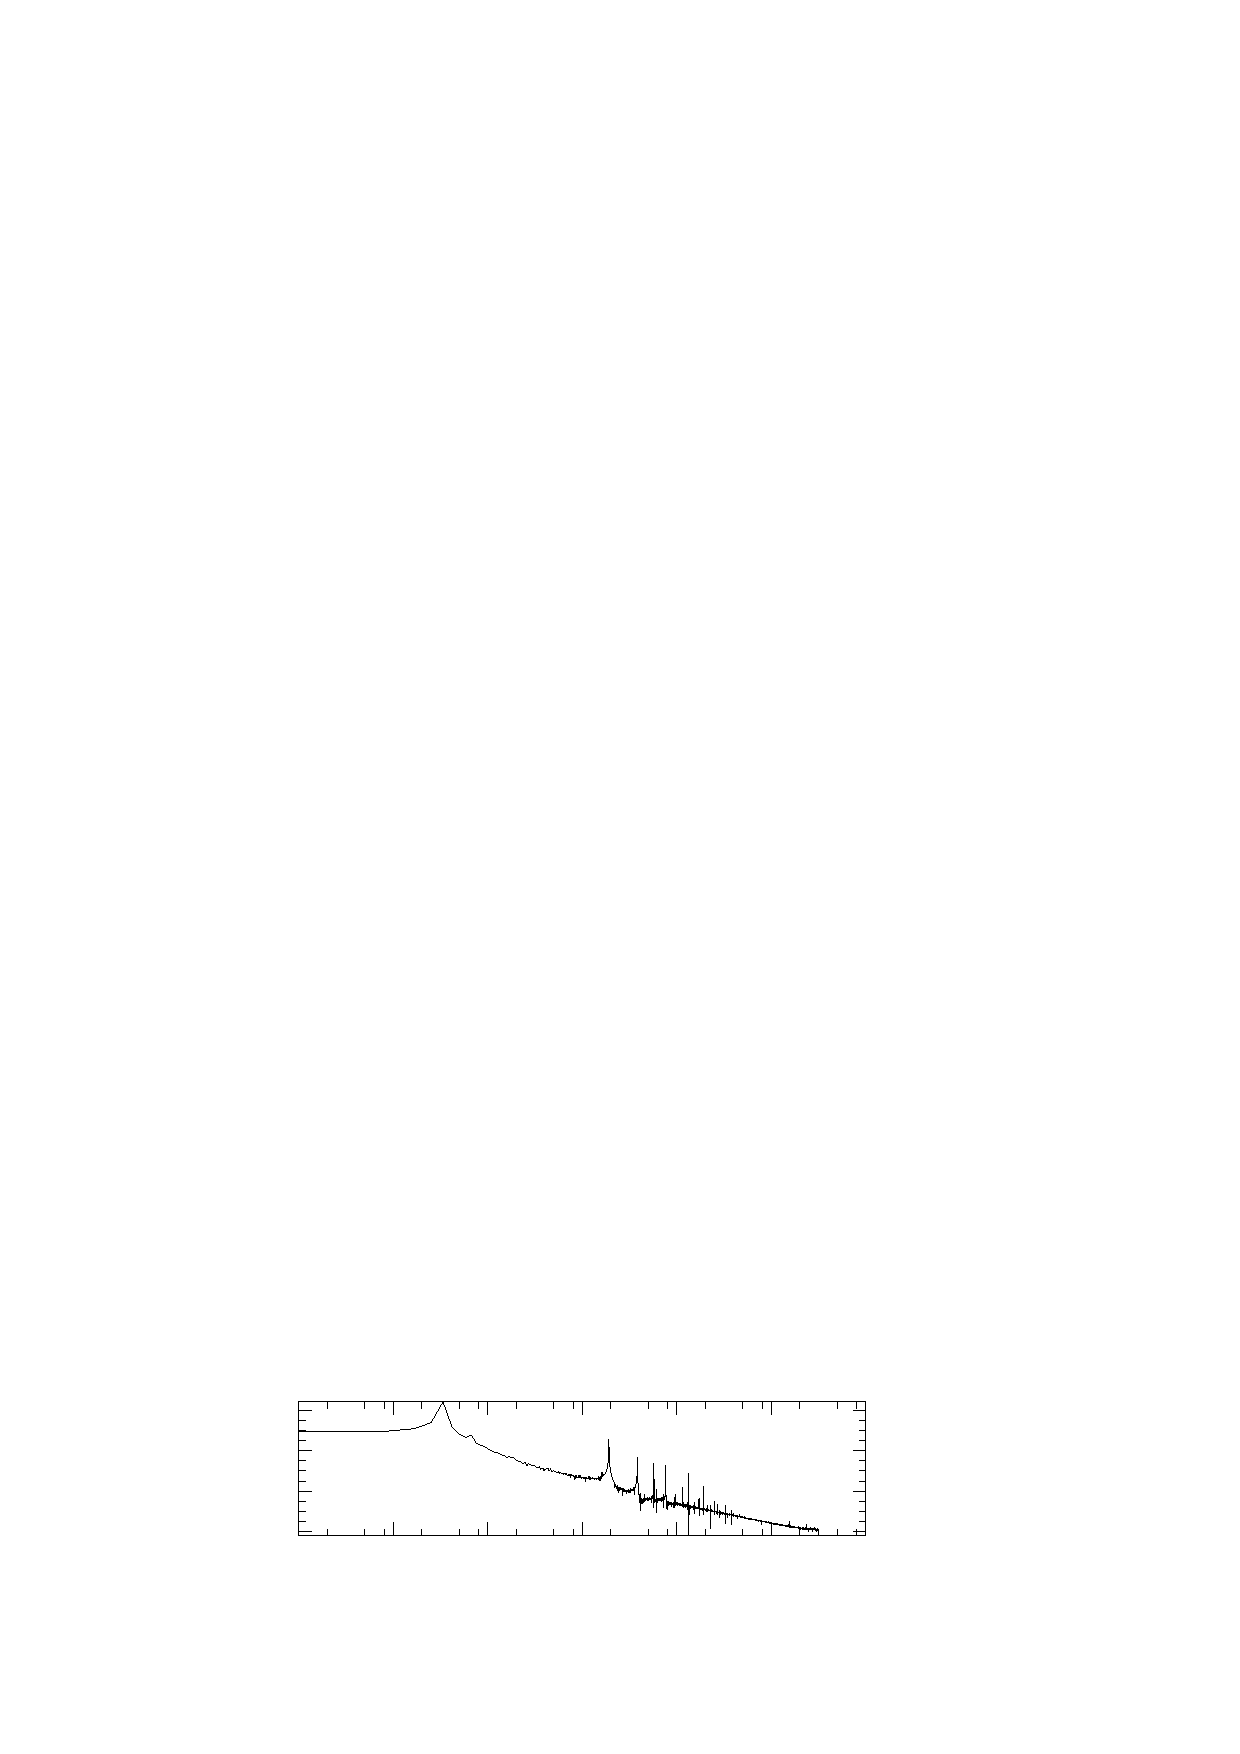
\includegraphics{rounded-rhop30-Fo7_508e-03-spectrum}%
%\end{picture}%
%\begingroup
%\setlength{\unitlength}{0.0200bp}%
%\begin{picture}(18000,5400)(0,0)%
%\put(3300,1750){\makebox(0,0)[r]{\strut{}1.00e-16}}%
%\put(3300,2712){\makebox(0,0)[r]{\strut{}1.00e-12}}%
%\put(3300,3674){\makebox(0,0)[r]{\strut{}1.00e-08}}%
%\put(3300,4636){\makebox(0,0)[r]{\strut{}1.00e-04}}%
%\put(3575,1100){\makebox(0,0){\strut{} 1e-05}}%
%\put(5842,1100){\makebox(0,0){\strut{} 1e-04}}%
%\put(8108,1100){\makebox(0,0){\strut{} 0.001}}%
%\put(10375,1100){\makebox(0,0){\strut{} 0.01}}%
%\put(12642,1100){\makebox(0,0){\strut{} 0.1}}%
%\put(14908,1100){\makebox(0,0){\strut{} 1}}%
%\put(17175,1100){\makebox(0,0){\strut{} 10}}%
%\put(550,3250){\rotatebox{90}{\makebox(0,0){\strut{}$PSD$}}}%
%\put(10375,275){\makebox(0,0){\strut{}$\omega$}}%
%\put(600,1000){\makebox(0,0){\strut{}(a)}}%
%\end{picture}%
%\endgroup
%\endinput

\caption{\label{fig:paths-rho-30-rounded}
Posici'on vertical de la part'icula s'olida $\rho_p/\rho_f=50$ sobre el tiempo en la cavidad redondeada para
(a) $P_o^\ast = 6.0\times 10^{-4} $ y (b) su espectro de potencia.
}
\end{figure}

\begin{figure}
%GNUPLOT: LaTeX picture with Postscript
\begin{picture}(0,0)%
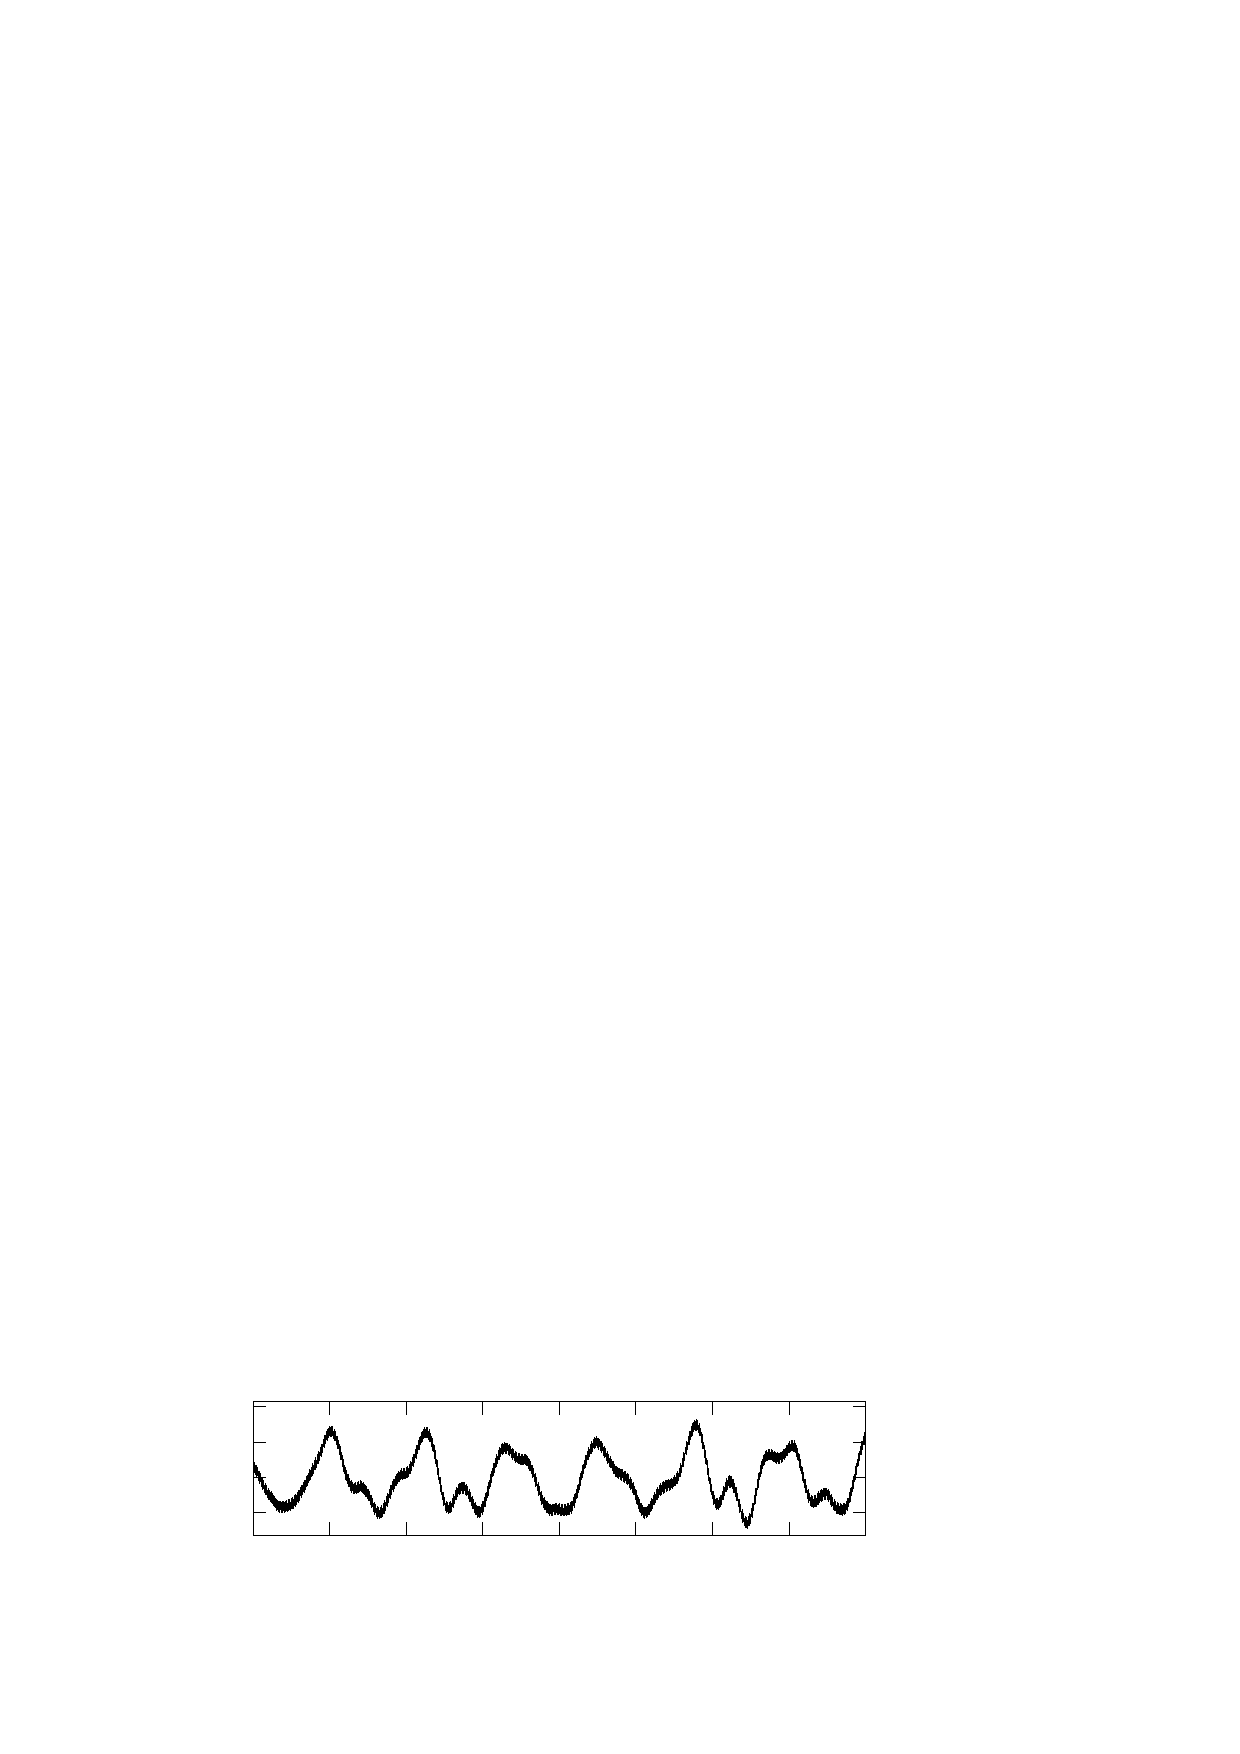
\includegraphics{rounded-rhop30-Fo5_631e-02}%
\end{picture}%
\begingroup
\setlength{\unitlength}{0.0200bp}%
\begin{picture}(18000,5400)(0,0)%
\put(2200,2193){\makebox(0,0)[r]{\strut{}1.40}}%
\put(2200,3040){\makebox(0,0)[r]{\strut{}1.50}}%
\put(2200,3887){\makebox(0,0)[r]{\strut{}1.60}}%
\put(2200,4734){\makebox(0,0)[r]{\strut{}1.70}}%
\put(2475,1100){\makebox(0,0){\strut{} 1600}}%
\put(4313,1100){\makebox(0,0){\strut{} 1650}}%
\put(6150,1100){\makebox(0,0){\strut{} 1700}}%
\put(7988,1100){\makebox(0,0){\strut{} 1750}}%
\put(9825,1100){\makebox(0,0){\strut{} 1800}}%
\put(11663,1100){\makebox(0,0){\strut{} 1850}}%
\put(13500,1100){\makebox(0,0){\strut{} 1900}}%
\put(15338,1100){\makebox(0,0){\strut{} 1950}}%
\put(17175,1100){\makebox(0,0){\strut{} 2000}}%
\put(550,3250){\rotatebox{90}{\makebox(0,0){\strut{}$y^\ast$}}}%
\put(9825,275){\makebox(0,0){\strut{}$t^\ast$}}%
\put(600,1000){\rotatebox{0}{\makebox(0,0){\strut{}(a)}}}%
\end{picture}%
\endgroup
\endinput

%%GNUPLOT: LaTeX picture with Postscript
%\begin{picture}(0,0)%
%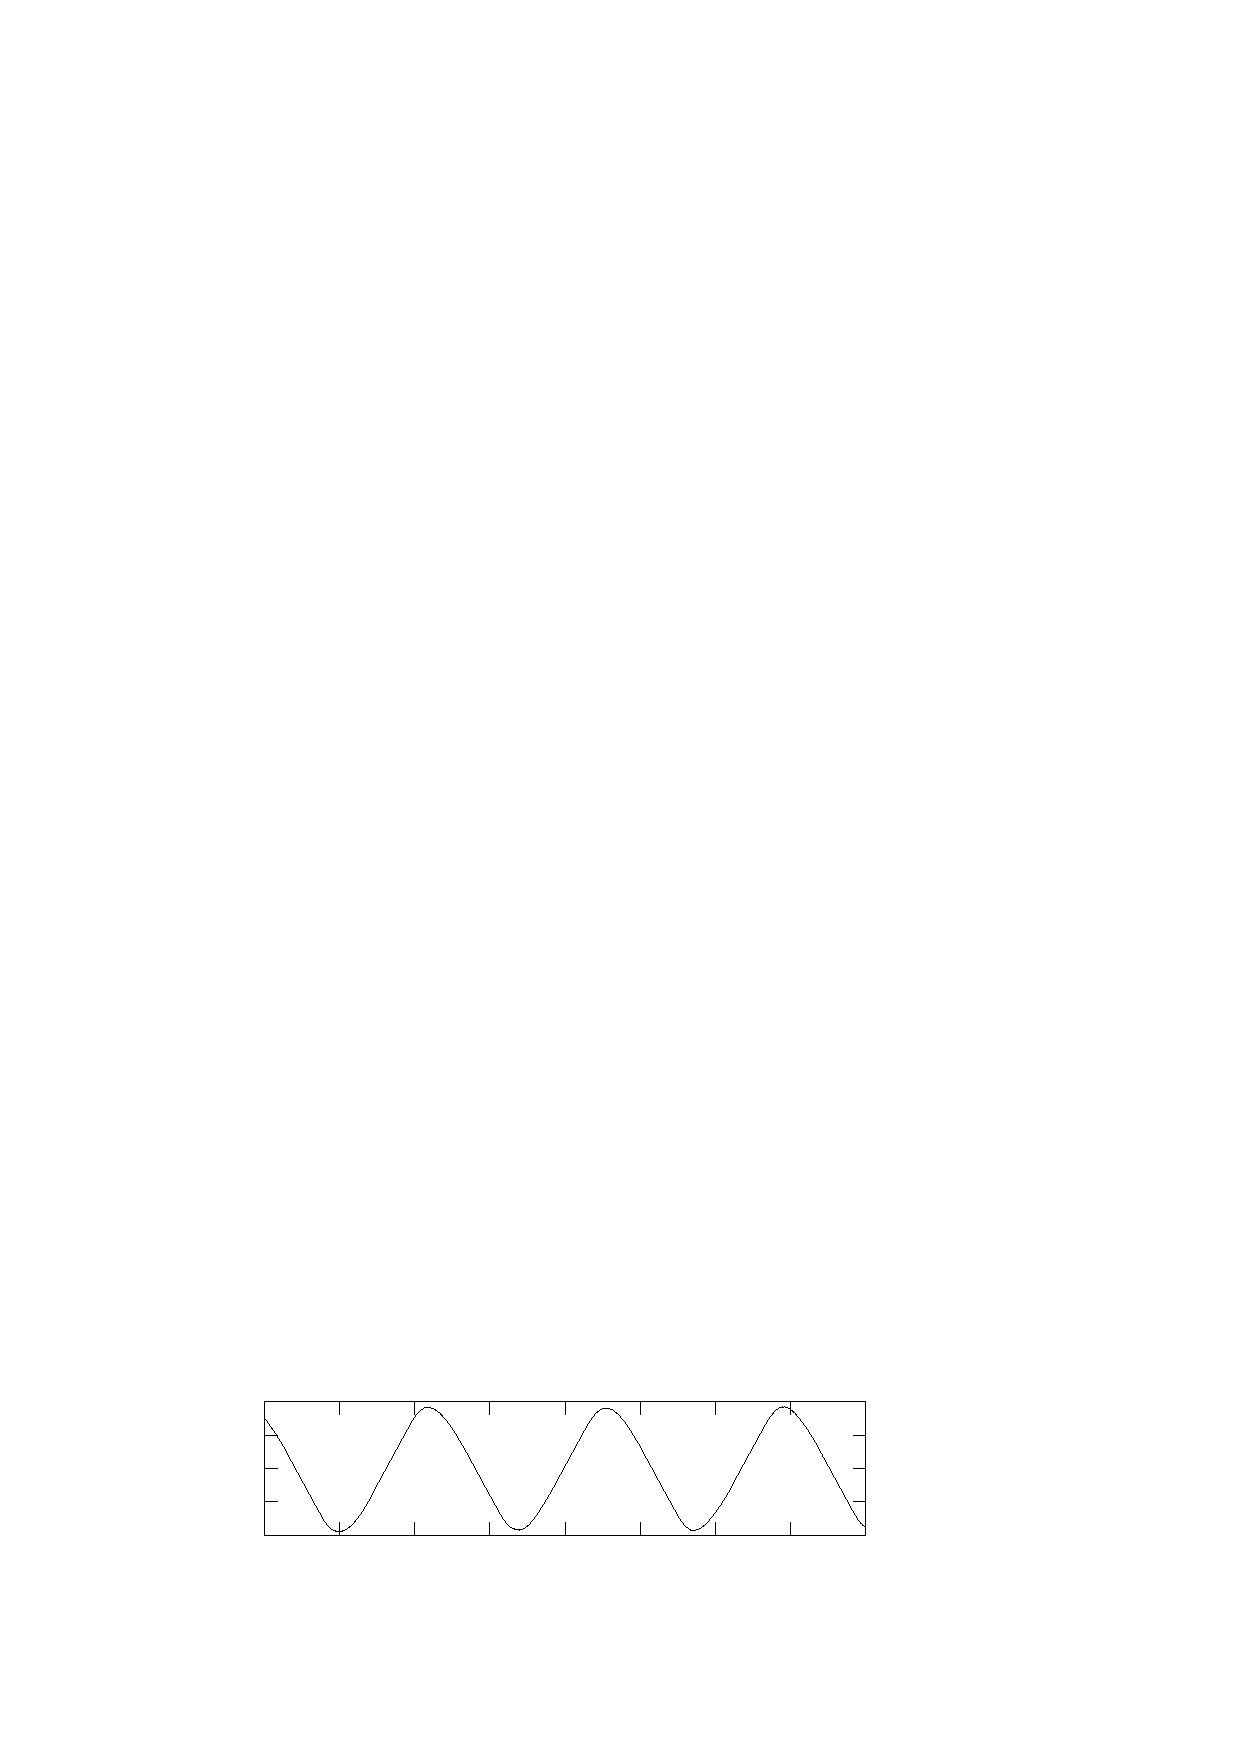
\includegraphics{rounded-rhop30-Fo5_631e-02-x}%
%\end{picture}%
%\begingroup
%\setlength{\unitlength}{0.0200bp}%
%\begin{picture}(18000,5400)(0,0)%
%\put(2475,1650){\makebox(0,0)[r]{\strut{}-1.60}}%
%\put(2475,2450){\makebox(0,0)[r]{\strut{}-0.80}}%
%\put(2475,3250){\makebox(0,0)[r]{\strut{}0.00}}%
%\put(2475,4050){\makebox(0,0)[r]{\strut{}0.80}}%
%\put(2475,4850){\makebox(0,0)[r]{\strut{}1.60}}%
%\put(2750,1100){\makebox(0,0){\strut{} 1600}}%
%\put(4553,1100){\makebox(0,0){\strut{} 1650}}%
%\put(6356,1100){\makebox(0,0){\strut{} 1700}}%
%\put(8159,1100){\makebox(0,0){\strut{} 1750}}%
%\put(9963,1100){\makebox(0,0){\strut{} 1800}}%
%\put(11766,1100){\makebox(0,0){\strut{} 1850}}%
%\put(13569,1100){\makebox(0,0){\strut{} 1900}}%
%\put(15372,1100){\makebox(0,0){\strut{} 1950}}%
%\put(17175,1100){\makebox(0,0){\strut{} 2000}}%
%\put(550,3250){\rotatebox{90}{\makebox(0,0){\strut{}$x^\ast$}}}%
%\put(9962,275){\makebox(0,0){\strut{}$t^\ast$}}%
%\put(600,1000){\rotatebox{0}{\makebox(0,0){\strut{}(b)}}}%
%\end{picture}%
%\endgroup
%\endinput

%GNUPLOT: LaTeX picture with Postscript
\begin{picture}(0,0)%
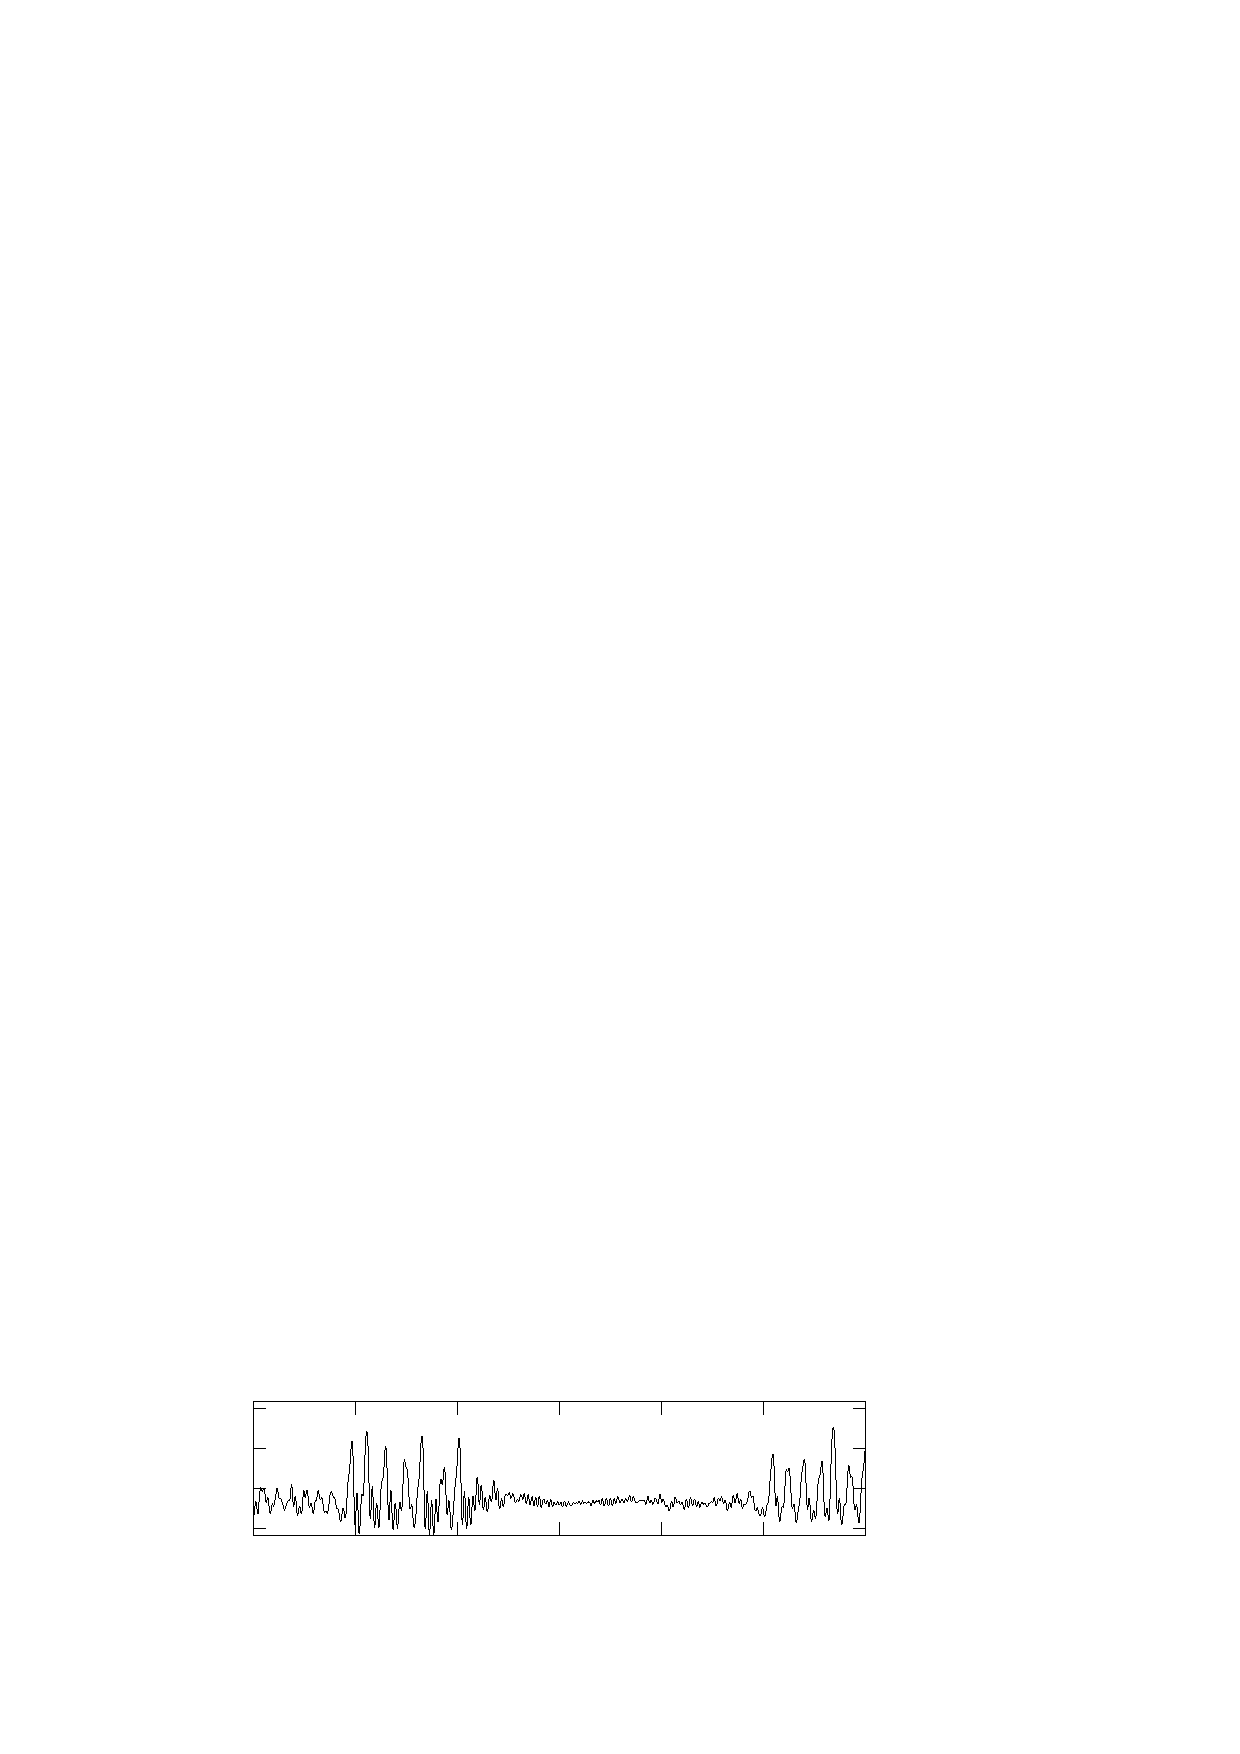
\includegraphics{rounded-rhop30-Fo8_072e-02}%
\end{picture}%
\begingroup
\setlength{\unitlength}{0.0200bp}%
\begin{picture}(18000,5400)(0,0)%
\put(2200,1805){\makebox(0,0)[r]{\strut{}1.20}}%
\put(2200,2765){\makebox(0,0)[r]{\strut{}1.60}}%
\put(2200,3725){\makebox(0,0)[r]{\strut{}2.00}}%
\put(2200,4685){\makebox(0,0)[r]{\strut{}2.40}}%
\put(2475,1100){\makebox(0,0){\strut{} 500}}%
\put(4925,1100){\makebox(0,0){\strut{} 1000}}%
\put(7375,1100){\makebox(0,0){\strut{} 1500}}%
\put(9825,1100){\makebox(0,0){\strut{} 2000}}%
\put(12275,1100){\makebox(0,0){\strut{} 2500}}%
\put(14725,1100){\makebox(0,0){\strut{} 3000}}%
\put(17175,1100){\makebox(0,0){\strut{} 3500}}%
\put(550,3250){\rotatebox{90}{\makebox(0,0){\strut{}$y^\ast$}}}%
\put(9825,275){\makebox(0,0){\strut{}$t^\ast$}}%
\put(600,1000){\rotatebox{0}{\makebox(0,0){\strut{}(c)}}}%
\end{picture}%
\endgroup
\endinput

%GNUPLOT: LaTeX picture with Postscript
\begin{picture}(0,0)%
\includegraphics{rounded-rhop30-Fo8_072e-02-x}%
\end{picture}%
\begingroup
\setlength{\unitlength}{0.0200bp}%
\begin{picture}(18000,5400)(0,0)%
\put(2475,1650){\makebox(0,0)[r]{\strut{}-2.80}}%
\put(2475,2450){\makebox(0,0)[r]{\strut{}-1.40}}%
\put(2475,3250){\makebox(0,0)[r]{\strut{}0.00}}%
\put(2475,4050){\makebox(0,0)[r]{\strut{}1.40}}%
\put(2475,4850){\makebox(0,0)[r]{\strut{}2.80}}%
\put(3652,1100){\makebox(0,0){\strut{} 500}}%
\put(5905,1100){\makebox(0,0){\strut{} 1000}}%
\put(8159,1100){\makebox(0,0){\strut{} 1500}}%
\put(10413,1100){\makebox(0,0){\strut{} 2000}}%
\put(12667,1100){\makebox(0,0){\strut{} 2500}}%
\put(14921,1100){\makebox(0,0){\strut{} 3000}}%
\put(17175,1100){\makebox(0,0){\strut{} 3500}}%
\put(550,3250){\rotatebox{90}{\makebox(0,0){\strut{}$x^\ast$}}}%
\put(9962,275){\makebox(0,0){\strut{}$t^\ast$}}%
\put(600,1000){\rotatebox{0}{\makebox(0,0){\strut{}(d)}}}%
\end{picture}%
\endgroup
\endinput

\caption{\label{fig:paths-rho-30-rounded-b}
(a) Posici'on vertical y 
(b) horizontal sobre el tiempo para  $P_o^\ast = 4.5\times 10^{-3}$
y
(c) posici'on vertical y 
(d) horizontal sobre el tiempo para  $P_o^\ast = 6.45\times 10^{-3}$.
}
\end{figure}

\begin{figure} 
%\put(15400,4350){\makebox(0,0)[r]{\strut{}(b)}}%
%estan ~gbv/doctorado/levitation/particle/flat-cavity/spectrum/barrido-rho
%%GNUPLOT: LaTeX picture with Postscript
%\begin{picture}(0,0)%
%\includegraphics{rounded-rhop30-Fo7_508e-03-spectrum}%
%\end{picture}%
%\begingroup
%\setlength{\unitlength}{0.0200bp}%
%\begin{picture}(18000,5400)(0,0)%
%\put(3300,1750){\makebox(0,0)[r]{\strut{}1.00e-16}}%
%\put(3300,2712){\makebox(0,0)[r]{\strut{}1.00e-12}}%
%\put(3300,3674){\makebox(0,0)[r]{\strut{}1.00e-08}}%
%\put(3300,4636){\makebox(0,0)[r]{\strut{}1.00e-04}}%
%\put(3575,1100){\makebox(0,0){\strut{} 1e-05}}%
%\put(5842,1100){\makebox(0,0){\strut{} 1e-04}}%
%\put(8108,1100){\makebox(0,0){\strut{} 0.001}}%
%\put(10375,1100){\makebox(0,0){\strut{} 0.01}}%
%\put(12642,1100){\makebox(0,0){\strut{} 0.1}}%
%\put(14908,1100){\makebox(0,0){\strut{} 1}}%
%\put(17175,1100){\makebox(0,0){\strut{} 10}}%
%\put(550,3250){\rotatebox{90}{\makebox(0,0){\strut{}$PSD$}}}%
%\put(10375,275){\makebox(0,0){\strut{}$\omega$}}%
%\put(600,1000){\makebox(0,0){\strut{}(a)}}%
%\end{picture}%
%\endgroup
%\endinput

%%GNUPLOT: LaTeX picture with Postscript
\begin{picture}(0,0)%
\includegraphics{rounded-rhop30-Fo3_191e-02-spectrum}%
\end{picture}%
\begingroup
\setlength{\unitlength}{0.0200bp}%
\begin{picture}(18000,5400)(0,0)%
\put(3300,2123){\makebox(0,0)[r]{\strut{}3.20e-14}}%
\put(3300,2997){\makebox(0,0)[r]{\strut{}1.60e-11}}%
\put(3300,3871){\makebox(0,0)[r]{\strut{}8.00e-09}}%
\put(3300,4745){\makebox(0,0)[r]{\strut{}4.00e-06}}%
\put(3575,1100){\makebox(0,0){\strut{} 1e-05}}%
\put(5842,1100){\makebox(0,0){\strut{} 1e-04}}%
\put(8108,1100){\makebox(0,0){\strut{} 0.001}}%
\put(10375,1100){\makebox(0,0){\strut{} 0.01}}%
\put(12642,1100){\makebox(0,0){\strut{} 0.1}}%
\put(14908,1100){\makebox(0,0){\strut{} 1}}%
\put(17175,1100){\makebox(0,0){\strut{} 10}}%
\put(550,3250){\rotatebox{90}{\makebox(0,0){\strut{}$PSD$}}}%
\put(10375,275){\makebox(0,0){\strut{}$\omega$}}%
\end{picture}%
\endgroup
\endinput

%%GNUPLOT: LaTeX picture with Postscript
%\begin{picture}(0,0)%
%\includegraphics{rounded-rhop30-Fo5_631e-02-spectrum}%
%\end{picture}%
%\begingroup
%\setlength{\unitlength}{0.0200bp}%
%\begin{picture}(18000,5400)(0,0)%
%\put(3300,1850){\makebox(0,0)[r]{\strut{}3.20e-14}}%
%\put(3300,2601){\makebox(0,0)[r]{\strut{}1.60e-11}}%
%\put(3300,3352){\makebox(0,0)[r]{\strut{}8.00e-09}}%
%\put(3300,4103){\makebox(0,0)[r]{\strut{}4.00e-06}}%
%\put(3575,1100){\makebox(0,0){\strut{} 1e-05}}%
%\put(5842,1100){\makebox(0,0){\strut{} 1e-04}}%
%\put(8108,1100){\makebox(0,0){\strut{} 0.001}}%
%\put(10375,1100){\makebox(0,0){\strut{} 0.01}}%
%\put(12642,1100){\makebox(0,0){\strut{} 0.1}}%
%\put(14908,1100){\makebox(0,0){\strut{} 1}}%
%\put(17175,1100){\makebox(0,0){\strut{} 10}}%
%\put(550,3250){\rotatebox{90}{\makebox(0,0){\strut{}$PSD$}}}%
%\put(10375,275){\makebox(0,0){\strut{}$\omega$}}%
%\put(600,1000){\makebox(0,0){\strut{}(b)}}%
%\end{picture}%
%\endgroup
%\endinput

%%GNUPLOT: LaTeX picture with Postscript
%\begin{picture}(0,0)%
%\includegraphics{rounded-rhop30-Fo8_072e-02-spectrum}%
%\end{picture}%
%\begingroup
%\setlength{\unitlength}{0.0200bp}%
%\begin{picture}(18000,5400)(0,0)%
%\put(3300,1692){\makebox(0,0)[r]{\strut{}3.20e-14}}%
%\put(3300,2476){\makebox(0,0)[r]{\strut{}1.60e-11}}%
%\put(3300,3260){\makebox(0,0)[r]{\strut{}8.00e-09}}%
%\put(3300,4044){\makebox(0,0)[r]{\strut{}4.00e-06}}%
%\put(3300,4829){\makebox(0,0)[r]{\strut{}2.00e-03}}%
%\put(3575,1100){\makebox(0,0){\strut{} 1e-05}}%
%\put(5842,1100){\makebox(0,0){\strut{} 1e-04}}%
%\put(8108,1100){\makebox(0,0){\strut{} 0.001}}%
%\put(10375,1100){\makebox(0,0){\strut{} 0.01}}%
%\put(12642,1100){\makebox(0,0){\strut{} 0.1}}%
%\put(14908,1100){\makebox(0,0){\strut{} 1}}%
%\put(17175,1100){\makebox(0,0){\strut{} 10}}%
%\put(550,3250){\rotatebox{90}{\makebox(0,0){\strut{}$PSD$}}}%
%\put(10375,275){\makebox(0,0){\strut{}$\omega$}}%
%\put(600,1000){\rotatebox{0}{\makebox(0,0){\strut{}(c)}}}%
%\end{picture}%
%\endgroup
%\endinput

\caption{\label{fig:paths-rho-30-rounded-spectrum}
Espectro de potencia del movimiento vertical de la part'icula s'olida $\rho_p/\rho_f=50$ sobre el tiempo en la cavidad redondeada para
(a) $P_o^\ast = 6.0\times 10^{-4} $,
%(b) $P_o^\ast = 2.55\times 10^{-3}$,
(b) $P_o^\ast = 4.5\times 10^{-3}$
y
(c) $P_o^\ast = 6.45\times 10^{-3}$. Los espectros corresponden al movimiento de las part'iculas mostradas en las 
figuras~\ref{fig:paths-rho-30-rounded} (a),~\ref{fig:paths-rho-30-rounded-b} (a) y (c).
}
\end{figure}
%
\begin{figure} 
%GNUPLOT: LaTeX picture with Postscript
\begin{picture}(0,0)%
\includegraphics{eps/rounded-rhop30-Fo5_631e-02-x-y}%
\end{picture}%
\begingroup
\setlength{\unitlength}{0.0200bp}%
\begin{picture}(18000,5400)(0,0)%
\put(2200,1650){\makebox(0,0)[r]{\strut{}1.30}}%
\put(2200,2450){\makebox(0,0)[r]{\strut{}1.40}}%
\put(2200,3250){\makebox(0,0)[r]{\strut{}1.50}}%
\put(2200,4050){\makebox(0,0)[r]{\strut{}1.60}}%
\put(2200,4850){\makebox(0,0)[r]{\strut{}1.70}}%
\put(2934,1100){\makebox(0,0){\strut{}-1.5}}%
\put(5231,1100){\makebox(0,0){\strut{}-1}}%
\put(7528,1100){\makebox(0,0){\strut{}-0.5}}%
\put(9825,1100){\makebox(0,0){\strut{} 0}}%
\put(12122,1100){\makebox(0,0){\strut{} 0.5}}%
\put(14419,1100){\makebox(0,0){\strut{} 1}}%
\put(16716,1100){\makebox(0,0){\strut{} 1.5}}%
\put(550,3250){\rotatebox{90}{\makebox(0,0){\strut{}$y^\ast$}}}%
\put(9825,275){\makebox(0,0){\strut{}$x^\ast$}}%
\put(600,1000){\rotatebox{0}{\makebox(0,0){\strut{}(a)}}}%
\end{picture}%
\endgroup
\endinput

%%GNUPLOT: LaTeX picture with Postscript
%\begin{picture}(0,0)%
%\includegraphics{rounded-rhop30-Fo8_072e-02-x-y}%
%\end{picture}%
%\begingroup
%\setlength{\unitlength}{0.0200bp}%
%\begin{picture}(18000,5400)(0,0)%
%\put(2200,1764){\makebox(0,0)[r]{\strut{}1.05}}%
%\put(2200,2564){\makebox(0,0)[r]{\strut{}1.40}}%
%\put(2200,3364){\makebox(0,0)[r]{\strut{}1.75}}%
%\put(2200,4164){\makebox(0,0)[r]{\strut{}2.10}}%
%\put(4575,1100){\makebox(0,0){\strut{}-2}}%
%\put(7200,1100){\makebox(0,0){\strut{}-1}}%
%\put(9825,1100){\makebox(0,0){\strut{} 0}}%
%\put(12450,1100){\makebox(0,0){\strut{} 1}}%
%\put(15075,1100){\makebox(0,0){\strut{} 2}}%
%\put(550,3250){\rotatebox{90}{\makebox(0,0){\strut{}$y^\ast$}}}%
%\put(9825,275){\makebox(0,0){\strut{}$x^\ast$}}%
%\put(600,1000){\rotatebox{0}{\makebox(0,0){\strut{}(b)}}}%
%\end{picture}%
%\endgroup
%\endinput

\caption{\label{fig:paths-rho-30-rounded-x-y} 
Trayectoria en el plano $x-y$ de la part'icula s'olida en la cavidad redondeada  para
(a) $P_o^\ast = 4.5\times 10^{-3}$
y
(b) $P_o^\ast = 6.45\times 10^{-3}$. Las trayectorias corresponden a las mostradas en las 
figuras~\ref{fig:paths-rho-30-rounded-b} (a) y (c), respectivamente.
}
\end{figure}


En la figura~\ref{fig:paths-rho-30-rounded} (a) mostramos la posici'on vertical de la part'icula
para la cavidad redondeada para  $\rho_p/\rho_f = 50$ y  $P_o^\ast = 6.0\times 10^{-4} $. De
esta figura observamos que la part'icula oscila con dos frecuencias, como lo
comprobamos en la figura~\ref{fig:paths-rho-30-rounded} (b), donde mostramos el espectro
de potencia para esa trayectoria. Para este valor de $P_o^\ast$ la part'icula sigue una 
trayectoria dominada por dos frecuencias y sus arm'onicos y no presenta movimiento en la
direcci'on horizontal. En las figuras~\ref{fig:paths-rho-30-rounded-b} (a) y (b) mostramos
el movimiento de la part'icula en la cavidad redondeada para el eje vertical y 
horizontal, respectivamente, para $P_o^\ast = 4.5 \times 10^{-3}$. Para este valor 
de $P_o^\ast$ la part'icula presenta un movimiento horizontal regular, como podemos observar
de estas dos figuras. De la figura~\ref{fig:paths-rho-30-rounded-spectrum} (b), que es el
espectro de potencia para la trajectoria vertical, observamos que el movimiento de la part'icula
sigue siendo dominado por dos frecuecias y sus arm'onicos, siendo una de ellas la frecuencia
de oscilaci'on de la fuente ac'ustica.
En las figuras~\ref{fig:paths-rho-30-rounded-b} (c) y (d) mostramos
el movimiento vertical y horizontal de la part'icula para $P_o^\ast = 6.45\times 10^{-3}$. 
El movimiento horizontal de la part'icula est'a fuertemente correlacionado con el vertical, como 
puede verse. La part'icula oscila horizontalmente cerca del
nodo de presi'on derecho, luego oscila entre los dos nodos para luego oscilar cerca del nodo de 
presi'on derecho. Correspondientemente, las oscilaciones verticales son peque~nas, se ampl'ian
cuando la oscilaci'on horizontal pasa del lado izquierdo al lado derecho de la cavidad y es peque~na
cuando la posici'on horizontal vuelve a oscilar alrededor de un nodo. Este comportamiento se repite
sin periodicidad aparente, y sabemos que un comportamiento ca'otico se caracteriza por su
aperiodicidad y su sensibilidad respecto a condiciones iniciales~\cite{strogatzbook}. La primera
caracter'istica se cumple y la sensibilidad respecto a condiciones iniciales puede establecerse
del c'omputo num'erico del exponente de Lyapunov, que se obtiene de la serie temporal de la
posici'on horizontal o vertical de la part'icula~\cite{kantzbook}. Encontramos que el exponente de Lyapunov
tiene un valor de $0.05$ que es demasiado peque~no para concluir con certeza que el movimiento de la part'icula
en este caso es ca'otico. Lo que podemos afirmar, es que se trata de una oscilaci'on compleja y que
puede existir un caos transiente~\cite{strogatzbook} o un comportamiento complejo a'un cuando el exponente
de Lyapunov sea cero.
En la   figura~\ref{fig:paths-rho-30-rounded-spectrum} (c) mostramos el espectro de potencia
de la oscilaci'on vertical para $P^\ast_o=6.54\times 10^{-3}$, donde podemos identificar
la frecuencia de la fuente ac'ustica y sus arm'onicos y no es posible identificar una 'unica frecuencia
menor que la de la fuente ac'ustica como en muchos de los resultados anteriores.


En las figuras~\ref{fig:paths-rho-30-rounded-x-y} (a) y (b) mostramos las trayectorias en 
en plano $x-y$ para $P^\ast_o=4.50\times 10^{-3}$ y  $P^\ast_o=6.45\times 10^{-3}$.
La primera es una trayectoria regular, mientras que la segunda parece ca'otica. 
Vemos unas manchas oscura en la  figura~\ref{fig:paths-rho-30-rounded-x-y} (b) 
donde la part'icula permanece m'as tiempo, ubicadas en $(-1.4,1.5)$ y  $(1.4,1.5)$.

\begin{figure} 
\hskip -3.cm
%%GNUPLOT: LaTeX picture with Postscript
%\begin{picture}(0,0)%
%\includegraphics{variaciones-P-rho-30-Fo7_5e-03}%
%\end{picture}%
%\begingroup
%\setlength{\unitlength}{0.0200bp}%
%\begin{picture}(14400,8640)(0,0)%
%\put(10336,4426){\makebox(0,0)[l]{\strut{}1.000}}%
%\put(10336,5092){\makebox(0,0)[l]{\strut{}1.003}}%
%\put(10336,5757){\makebox(0,0)[l]{\strut{}1.005}}%
%\put(10336,6423){\makebox(0,0)[l]{\strut{}1.008}}%
%\put(9038,2206){\makebox(0,0){\strut{}-6}}%
%\put(8426,2206){\makebox(0,0){\strut{}-4}}%
%\put(7812,2206){\makebox(0,0){\strut{}-2}}%
%\put(7200,2206){\makebox(0,0){\strut{} 0}}%
%\put(6587,2206){\makebox(0,0){\strut{} 2}}%
%\put(5974,2206){\makebox(0,0){\strut{} 4}}%
%\put(5361,2206){\makebox(0,0){\strut{} 6}}%
%\put(5086,3063){\makebox(0,0)[r]{\strut{} 0}}%
%\put(5086,3676){\makebox(0,0)[r]{\strut{} 2}}%
%\put(5087,4289){\makebox(0,0)[r]{\strut{} 4}}%
%\put(5087,4901){\makebox(0,0)[r]{\strut{} 6}}%
%\put(5087,5514){\makebox(0,0)[r]{\strut{} 8}}%
%\put(5087,6127){\makebox(0,0)[r]{\strut{} 10}}%
%\put(7200,1206){\makebox(0,0){\strut{} $x^\ast$}}%
%\put(4087,4289){\makebox(0,0)[r]{\strut{} $y^\ast$}}%
%\put(12000,206){\makebox(0,0){\strut{} (a)}}%
%\end{picture}%
%\endgroup
%\endinput
 
\hskip -3.1cm
%%GNUPLOT: LaTeX picture with Postscript
%\begin{picture}(0,0)%
%\includegraphics{variaciones-U-rho-30-Fo7_5e-03}%
%\end{picture}%
%\begingroup
%\setlength{\unitlength}{0.0200bp}%
%\begin{picture}(14400,8640)(0,0)%
%\put(10336,4054){\makebox(0,0)[l]{\strut{}0.00}}%
%\put(10336,4646){\makebox(0,0)[l]{\strut{}0.25}}%
%\put(10336,5238){\makebox(0,0)[l]{\strut{}0.50}}%
%\put(10336,5830){\makebox(0,0)[l]{\strut{}0.75}}%
%\put(10336,6422){\makebox(0,0)[l]{\strut{}1.00}}%
%\put(9038,2206){\makebox(0,0){\strut{}-6}}%
%\put(8426,2206){\makebox(0,0){\strut{}-4}}%
%\put(7812,2206){\makebox(0,0){\strut{}-2}}%
%\put(7200,2206){\makebox(0,0){\strut{} 0}}%
%\put(6587,2206){\makebox(0,0){\strut{} 2}}%
%\put(5974,2206){\makebox(0,0){\strut{} 4}}%
%\put(5361,2206){\makebox(0,0){\strut{} 6}}%
%\put(5086,3063){\makebox(0,0)[r]{\strut{} 0}}%
%\put(5086,3676){\makebox(0,0)[r]{\strut{} 2}}%
%\put(5087,4289){\makebox(0,0)[r]{\strut{} 4}}%
%\put(5087,4901){\makebox(0,0)[r]{\strut{} 6}}%
%\put(5087,5514){\makebox(0,0)[r]{\strut{} 8}}%
%\put(5087,6127){\makebox(0,0)[r]{\strut{} 10}}%
%
%\put(7200,1206){\makebox(0,0){\strut{} $x^\ast$}}%
%\put(4087,4289){\makebox(0,0)[r]{\strut{} $y^\ast$}}%
%\end{picture}
%\endgroup
%\endinput
 

\hskip -3.cm
%%GNUPLOT: LaTeX picture with Postscript
%\begin{picture}(0,0)%
%\includegraphics{variaciones-P-rho-30-Fo5_6e-02}%
%\end{picture}%
%\begingroup
%\setlength{\unitlength}{0.0200bp}%
%\begin{picture}(14400,8640)(0,0)%
%\put(10336,4623){\makebox(0,0)[l]{\strut{}1.016}}%
%\put(10336,5219){\makebox(0,0)[l]{\strut{}1.039}}%
%\put(10336,5815){\makebox(0,0)[l]{\strut{}1.061}}%
%\put(10336,6410){\makebox(0,0)[l]{\strut{}1.084}}%
%\put(9038,2206){\makebox(0,0){\strut{}-6}}%
%\put(8426,2206){\makebox(0,0){\strut{}-4}}%
%\put(7812,2206){\makebox(0,0){\strut{}-2}}%
%\put(7200,2206){\makebox(0,0){\strut{} 0}}%
%\put(6587,2206){\makebox(0,0){\strut{} 2}}%
%\put(5974,2206){\makebox(0,0){\strut{} 4}}%
%\put(5361,2206){\makebox(0,0){\strut{} 6}}%
%\put(5086,3063){\makebox(0,0)[r]{\strut{} 0}}%
%\put(5086,3676){\makebox(0,0)[r]{\strut{} 2}}%
%\put(5087,4289){\makebox(0,0)[r]{\strut{} 4}}%
%\put(5087,4901){\makebox(0,0)[r]{\strut{} 6}}%
%\put(5087,5514){\makebox(0,0)[r]{\strut{} 8}}%
%\put(5087,6127){\makebox(0,0)[r]{\strut{} 10}}%
%
%\put(7200,1206){\makebox(0,0){\strut{} $x^\ast$}}%
%\put(4087,4289){\makebox(0,0)[r]{\strut{} $y^\ast$}}%
%\put(12000,206){\makebox(0,0){\strut{} (b)}}%
%\end{picture}%
%\endgroup
%\endinput
 
\hskip -3.1cm
%%GNUPLOT: LaTeX picture with Postscript
%\begin{picture}(0,0)%
%\includegraphics{variaciones-U-rho-30-Fo5_6e-02}%
%\end{picture}%
%\begingroup
%\setlength{\unitlength}{0.0200bp}%
%\begin{picture}(14400,8640)(0,0)%
%\put(10336,4054){\makebox(0,0)[l]{\strut{}0.00}}%
%\put(10336,4646){\makebox(0,0)[l]{\strut{}0.25}}%
%\put(10336,5238){\makebox(0,0)[l]{\strut{}0.50}}%
%\put(10336,5830){\makebox(0,0)[l]{\strut{}0.75}}%
%\put(10336,6422){\makebox(0,0)[l]{\strut{}1.00}}%
%\put(9038,2206){\makebox(0,0){\strut{}-6}}%
%\put(8426,2206){\makebox(0,0){\strut{}-4}}%
%\put(7812,2206){\makebox(0,0){\strut{}-2}}%
%\put(7200,2206){\makebox(0,0){\strut{} 0}}%
%\put(6587,2206){\makebox(0,0){\strut{} 2}}%
%\put(5974,2206){\makebox(0,0){\strut{} 4}}%
%\put(5361,2206){\makebox(0,0){\strut{} 6}}%
%\put(5086,3063){\makebox(0,0)[r]{\strut{} 0}}%
%\put(5086,3676){\makebox(0,0)[r]{\strut{} 2}}%
%\put(5087,4289){\makebox(0,0)[r]{\strut{} 4}}%
%\put(5087,4901){\makebox(0,0)[r]{\strut{} 6}}%
%\put(5087,5514){\makebox(0,0)[r]{\strut{} 8}}%
%\put(5087,6127){\makebox(0,0)[r]{\strut{} 10}}%
%
%\put(7200,1206){\makebox(0,0){\strut{} $x^\ast$}}%
%\put(4087,4289){\makebox(0,0)[r]{\strut{} $y^\ast$}}%
%%\put(7200,1206){\makebox(0,0){\strut{} (a)}}%
%\end{picture}%
%\endgroup
%\endinput



\hskip -3.cm
%%GNUPLOT: LaTeX picture with Postscript
%\begin{picture}(0,0)%
%\includegraphics{variaciones-P-rho-30-Fo8_1e-02}%
%\end{picture}%
%\begingroup
%\setlength{\unitlength}{0.0200bp}%
%\begin{picture}(14400,8640)(0,0)%
%\put(10336,4530){\makebox(0,0)[l]{\strut{}1.012}}%
%\put(10336,5125){\makebox(0,0)[l]{\strut{}1.040}}%
%\put(10336,5719){\makebox(0,0)[l]{\strut{}1.068}}%
%\put(10336,6314){\makebox(0,0)[l]{\strut{}1.095}}%
%\put(9038,2206){\makebox(0,0){\strut{}-6}}%
%\put(8426,2206){\makebox(0,0){\strut{}-4}}%
%\put(7812,2206){\makebox(0,0){\strut{}-2}}%
%\put(7200,2206){\makebox(0,0){\strut{} 0}}%
%\put(6587,2206){\makebox(0,0){\strut{} 2}}%
%\put(5974,2206){\makebox(0,0){\strut{} 4}}%
%\put(5361,2206){\makebox(0,0){\strut{} 6}}%
%\put(5086,3063){\makebox(0,0)[r]{\strut{} 0}}%
%\put(5086,3676){\makebox(0,0)[r]{\strut{} 2}}%
%\put(5087,4289){\makebox(0,0)[r]{\strut{} 4}}%
%\put(5087,4901){\makebox(0,0)[r]{\strut{} 6}}%
%\put(5087,5514){\makebox(0,0)[r]{\strut{} 8}}%
%\put(5087,6127){\makebox(0,0)[r]{\strut{} 10}}%
%
%\put(7200,1206){\makebox(0,0){\strut{} $x^\ast$}}%
%\put(4087,4289){\makebox(0,0)[r]{\strut{} $y^\ast$}}%
%\put(12000,206){\makebox(0,0){\strut{} (c)}}%
%\end{picture}%
%\endgroup
%\endinput
 
\hskip -3.1cm
%%GNUPLOT: LaTeX picture with Postscript
%\begin{picture}(0,0)%
%\includegraphics{variaciones-U-rho-30-Fo8_1e-02}%
%\end{picture}%
%\begingroup
%\setlength{\unitlength}{0.0200bp}%
%\begin{picture}(14400,8640)(0,0)%
%\put(10336,4054){\makebox(0,0)[l]{\strut{}0.00}}%
%\put(10336,4646){\makebox(0,0)[l]{\strut{}0.25}}%
%\put(10336,5238){\makebox(0,0)[l]{\strut{}0.50}}%
%\put(10336,5830){\makebox(0,0)[l]{\strut{}0.75}}%
%\put(10336,6422){\makebox(0,0)[l]{\strut{}1.00}}%
%\put(9038,2206){\makebox(0,0){\strut{}-6}}%
%\put(8426,2206){\makebox(0,0){\strut{}-4}}%
%\put(7812,2206){\makebox(0,0){\strut{}-2}}%
%\put(7200,2206){\makebox(0,0){\strut{} 0}}%
%\put(6587,2206){\makebox(0,0){\strut{} 2}}%
%\put(5974,2206){\makebox(0,0){\strut{} 4}}%
%\put(5361,2206){\makebox(0,0){\strut{} 6}}%
%\put(5086,3063){\makebox(0,0)[r]{\strut{} 0}}%
%\put(5086,3676){\makebox(0,0)[r]{\strut{} 2}}%
%\put(5087,4289){\makebox(0,0)[r]{\strut{} 4}}%
%\put(5087,4901){\makebox(0,0)[r]{\strut{} 6}}%
%\put(5087,5514){\makebox(0,0)[r]{\strut{} 8}}%
%\put(5087,6127){\makebox(0,0)[r]{\strut{} 10}}%
%
%\put(7200,1206){\makebox(0,0){\strut{} $x^\ast$}}%
%\put(4087,4289){\makebox(0,0)[r]{\strut{} $y^\ast$}}%
%%\put(7200,1206){\makebox(0,0){\strut{} (a)}}%
%\end{picture}%
%\endgroup
%\endinput
 

\caption{\label{fig:potentials-rounded-rho-30}
Amplitud de las oscilaci'ones en la presi'on y la velocidad de izquierda a derecha para
(a) $P_o^\ast = 6.0\times 10^{-4} $,
%(b) $P_o^\ast = 2.55\times 10^{-3}$,
(b) $P_o^\ast = 4.5\times 10^{-3}$
y
(c) $P_o^\ast = 6.45\times 10^{-3}$.
}
\end{figure}
\begin{figure} 
%GNUPLOT: LaTeX picture with Postscript
\begin{picture}(0,0)%
\includegraphics{bifurcacion-rounded}%
\end{picture}%
\begingroup
\setlength{\unitlength}{0.0200bp}%
\begin{picture}(18000,5400)(0,0)%
\put(1650,1970){\makebox(0,0)[r]{\strut{}-2}}%
\put(1650,2610){\makebox(0,0)[r]{\strut{}-1}}%
\put(1650,3250){\makebox(0,0)[r]{\strut{}0}}%
\put(1650,3890){\makebox(0,0)[r]{\strut{}1}}%
\put(1650,4530){\makebox(0,0)[r]{\strut{}2}}%
\put(1925,1100){\makebox(0,0){\strut{}0.000}}%
\put(4104,1100){\makebox(0,0){\strut{}0.001}}%
\put(6282,1100){\makebox(0,0){\strut{}0.002}}%
\put(8461,1100){\makebox(0,0){\strut{}0.003}}%
\put(10639,1100){\makebox(0,0){\strut{}0.004}}%
\put(12818,1100){\makebox(0,0){\strut{}0.005}}%
\put(14996,1100){\makebox(0,0){\strut{}0.006}}%
\put(17175,1100){\makebox(0,0){\strut{}0.007}}%
\put(550,3250){\rotatebox{90}{\makebox(0,0){\strut{}$x^\ast$}}}%
\put(9550,275){\makebox(0,0){\strut{}$P_o^\ast$}}%
\end{picture}%
\endgroup
\endinput
 
\caption{\label{fig:bifurcacion-rounded}
Posici'on de los nodos de presi'on como funci'on de la cantidad de movimiento agregada por 
la fuente ac'ustica $P_o^\ast$ para la cavidad redondeada.
}
\end{figure}


Para identificar el origen del movimiento horizontal de la part'icula, mostramos las variaciones de las oscilaciones
en la presi'on y la velocidad en la cavidad redondeada.
En las figuras~\ref{fig:potentials-rounded-rho-30} (a), (b) y (c) mostramos la amplitud de las oscilaciones  locales
de la presi'on y velocidad para $P_o^\ast = 6.0\times 10^{-4} $, $P_o^\ast = 4.5\times 10^{-3}$
y $P_o^\ast = 6.45\times 10^{-3}$, respectivamente, donde nos interesa fundamentalmente 
el nodo de presi'on inferior. Al aumentar el valor de $P_o^\ast$, el nodo de presi'on inferior
se alarga horizontalmente (figura~\ref{fig:potentials-rounded-rho-30} (b)) para separarse en
dos (figura~\ref{fig:potentials-rounded-rho-30} (c)).	
 A pesar de la formaci'on de dos nodos de presi'on, no ocurre lo mismo con el antinodo de velocidad, 
sin embargo, las zonas donde se localizan los nuevos nodos de presi'on son zonas de alta velocidad. La aparici'on de estos
dos nodos de presi'on explica el movimiento irregular de la part'icula para $P^\ast_o = 6.45 \times 10^{-3}$.
En la figura~\ref{fig:bifurcacion-rounded} mostramos las posiciones horizontales de los
nodos de presi'on como funci'on de la cantidad de movimiento de la fuente ac'ustica. Vemos que podemos
identificar $P_{o_C}^\ast$ mencionada antes con el valor para el cual aparecen los dos nodos de presi'on.
Es la aparici'on de los dos nodos de presi'on lo que tambi'en propicia el complejo movimiento de la
part'icula en la cavidad redondeada.


\section{Conclusiones}
\label{sec:conclusiones}

La conclusi'on m'as importante es que el m'etodo de la ecuaci'on de Boltzmann en redes (EBR)
es capaz de resolver problemas de interacci'on de part'iculas s'olidas con fluidos compresibles,
en particular, el problema de la levitaci'on ac'ustica. Tambi'en, el m'etodo demostr'o ser capaz
de simular problemas con geometr'ias complicadas. En simulaciones num'ericas en ausencia de
un campo gravitacional externo, las part'iculas se dirigieron a los nodos de presi'on, tanto 
para la cavidad plana como para la redondeada.  Al agregar el campo gravitacional externo, la
part'icula en la cavidad plana tuvo un desplazamiento en su posici'on estacionaria
 mientras que la part'icula en la cavidad redondeada apenas si fue
notorio el desplazamiento. Esta diferencia se debe a que la fuerza ac'ustica en la cavidad
redondeada es mayor que en la cavidad plana.


Al mantener fija la cantidad de movimiento agregada por la fuente
ac'ustica y variar la relaci'on de densidades, la posici'on estacionaria de la part'icula se desplaz'o
linealmente en ambas cavidades aproximadamente entre $50< \rho_p/\rho_f <200$ con una pendiente
de $-0.001677$ para la cavidad plana y $-0.002274$ para la cavidad redondeada, por lo que
se concluye que la fuerza ac'ustica crece de manera lineal en una
peque~na zona. En la cavidad plana, la 
oscilaci'on vertical de la part'icula, medida con la desviaci'on est'andar, decrece al aumentar la relaci'on de
densidades. Para la cavidad redondeada, la oscilaci'on vertical de la part'icula decrece entre
 $2< \rho_p/\rho_f <50$, para luego incrementar su valor hasta alcanzar valores de $\sigma_y=0.36$.
Junto con el aumento de la oscilaci'on vertical, aparece un aumento en el valor de la 
velocidad m'axima del fluido dentro de la cavidad, evidencia de un  desplazamiento de la
frecuencia de resonancia debido a la presencia de la part'icula. Para el movimiento de la part'icula
en ambas cavidades hay dos tipos de movimiento de la part'icula. En el primero, la part'icula
oscila con la misma frecuencia de la fuente ac'ustica  y sus arm'onicos 
y con amplitud constante. En el segundo comportamiento, la part'icula oscila con frecuencia 
de la fuente ac'ustica y sus arm'onicos y aparece otra frecuencia mucho m'as baja. Cada frecuencia
tiene asociada una amplitud de oscilaci'on del movimiento de la part'icula, raz'on por la cual calculamos 
la desviaci'on est'andar del movimiento de la part'icula sobre el tiempo.


Al mantener fija la relaci'on de densidades de la part'icula en $\rho_p/\rho_f=50$ y variar la 
cantidad de movimiento agregada por la fuente, la part'icula se desplaz'o hacia el nodo de presi'on 
y aument'o el valor de la oscilaci'on vertical. En la cavidad redondeada, para $P_o^\ast >4\times 10^{-3}$, 
el valor de la oscilaci'on vertical $\sigma_y$ aument'o bruscamente y a la par, la part'icula comenz'o a presentar
un movimiento oscilatorio en el eje horizontal. Este comportamiento se debe a la divisi'on del nodo de 
presi'on. Para valores menores de la cantidad de movimiento agregada por la fuente ac'ustica, el nodo de presi'on
se encontraba en el centro horizontal de la cavidad, y para valores $P_o^\ast >4\times 10^{-3}$ existen dos
nodos de presi'on, ubicados en $(-2,1.5)$ y $(2,1.5)$. En todos los experimentos anteriores, la part'icula
hab'ia sido colocada en el centro de la cavidad $(0,1.5)$ para que alcanzara su posici'on estacionaria
r'apidamente.  Dado que la posici'on inicial es un punto inestable, la part'icula se movi'o entre un nodo de
presi'on y otro sin permanecer en alguno de los dos de manera preferencial. Sin embargo, el movimiento de la part'icula es inestable
independientemente de su posici'on inicial. Cuando la colocamos en uno de los nodos de presi'on $(-2,1.2)$ tambi'en
present'o movimientos oscilatorios en el eje horizontal y vertical alrededor de ambos nodos de presi'on.
El movimiento de la part'icula, para ambas cavidades, es funci'on de la cantidad de movimiento agregada 
por la fuente ac'ustica $P_o^\ast$ y la relaci'on de densidades entre la part'icula y el fluido $\rho_p/\rho_f$.
De los experimentos realizados al mantener fija la cantidad de movimiento y variar la relaci'on de las densidades
calculamos que la cavidad redondeada es m'as de cinco veces m'as efectiva que la cavidad plana para levitar
part'iculas m'as pesadas. Sin embargo, esta eficiencia tiene una consecuencia directa en la amplitud de la oscilaci'on
ya que las oscilaciones mayores se presentaron tambi'en en la cavidad redondeada. La aparici'on de los pares de 
nodos de presi'on es funci'on de la cantidad de movimiento agregado por la fuente ac'ustica y es exclusivo para 
la cavidad redondeada.

Al introducir la part'icula s'olida dentro de la cavidad redondeada, 'esta se sale de resonancia. La resonancia
es ahora funci'on no solo de la geometr'ia y frecuencia, sino del tama~no y posici'on de la part'icula s'olida.
En presencia de part'icula  el valor de la velocidad m'axima puede ser hasta 20\% m'as grande que en ausencia
de la part'icula. En las simulaciones presentadas en esta tesis se levitaron part'iculas con una relaci'on
m'axima de densidades de $\rho_p/\rho_f = 256$. La relaci'on de densidad entre el poliestireno y el aire
es $\rho_p/\rho_f=83$.

Para concluir, hacemos notar que hemos estudiado un peque~no espacio de par'ametros al variar la cantidad
de movimiento agregada por la fuente ac'ustica y la relaci'on de densidades entre la part'icula y el fluido.
El radio de la part'icula es tambi'en un par'ametro de gran importancia, sin embargo lo mantuvimos constante
en todas las simulaciones, as'i como los par'ametros geom'etricos de la cavidad redondeada. Demostramos 
que el m'etodo de la EBR es una herramienta 'util para estudiar num'ericamente una cavidad y optimizar el
par'ametro que se desee. Dado el peque~no espacio de par'ametros que hemos estudiado, encontramos que la
trayectoria de la part'icula puede ser muy compleja y encontramos evidencia de que puede ser ca'otica.

%\chapter{Conclusiones}


En esta tesis se presentamos la simulaci'on num'erica usando el m'etodo de la ecuaci'on
de Boltzmann en redes (EBR) de la levitaci'on ac'ustica de una part'icula s'olida circular
bidimensional en una cavidad con un reflector plano y otra con un reflector redondeado 
y concluimos que el m'etodo de la EBR es capaz de 
simular correctamente el problema de levitaci'on ac'ustica de una part'icula s'olida.

En el cap'itulo 2 presentamos como llegar a la ecuaci'on de Boltzmann en redes
para la malla $D2Q9$  a partir de la ecuaci'on de transporte de Boltzmann. Tambi'en
obtuvimos las ecuaciones hidrodin'amicas para un fluido compresible a partir de la 
EBR usando una expansi'on de Chapman-Enskog. Presentamos brevemente
la t'ecnica desarrollada por Aidun {\it et al}~\cite{aidun98} para la interacci'on
de part'iculas s'olidas con el m'etodo de la  ecuaci'on de Boltzmann en redes. Adem'as,
describimos el rebote hacia atr'as y el rebote hacia atr'as a mitad del camino para
recrear la condici'on de no deslizamiento en las paredes as'i como la manera
de agregar cantidad de movimiento para despu'es simular una fuente ac'ustica. 
Ambas condiciones de frontera  las utilizamos para la simulaci'on de la levitaci'on ac'ustica.
La validaci'on del m'etodo de la EBR se present'o en el ap'endice A, donde estudiamos tres
problemas y comparamos los resultados de las simulaciones num'ericas con los reportados
en la literatura.


En el cap'itulo 3 presentamos los antecedentes de la levitaci'on ac'ustica y resultados
de las simulaciones.
Los trabajos de King~\cite{king34} y Gor'kov~\cite{gorkov62} fueron la base 
para el comienzo del desarrollo de la teor'ia de la fuerza ac'ustica actuando
sobre una esfera. Realizamos simulaciones num'ericas de la levitaci'on 
ac'ustica en dos cavidades, una con un reflector plano, y la otra con un reflector
redondeado optimizado para aumentar la fuerza del campo ac'ustico~\cite{xie01}.
Encontramos los dos primeros modos resonantes para la cavidad redondeada monitoreando
el valor de la velocidad m'axima. Todos los experimentos para ambas
cavidades los realizamos en el segundo modo resonante. Los valores de las frecuencias de resonancia 
encontrados difieren a los reportados por
Xie {\it et al}. Esta diferencia es porque las simulaciones num'ericas las realizamos
en dos dimensiones mientras que lo reportado por Xie {\it et al} es para una cavidad
en tres dimensiones. Comprobamos
que en ausencia de gravedad, las part'iculas se dirigen al nodo de presi'on en ambas
cavidades, donde la
sumatoria de fuerzas ac'usticas es cero. En el segundo conjunto de simulaciones
mantuvimos constante la cantidad de movimiento agregada por la fuente ac'ustica
y variamos la  relaci'on de densidades entre la part'icula y el fluido. 
La posici'on de equilibrio de la part'icula, para ambas cavidades,
se fue desplazando hacia abajo. En una peque~na zona, el desplazamiento de la 
posici'on de equilibri'o sigui'o una l'inea recta. En la cavidad plana, las oscilaciones en el eje vertical
disminuyen conforme la relaci'on de densidades aumenta, pero para la cavidad 
redondeada, hay una zona donde la oscilaci'on de la part'icula en el eje vertical aumenta.
Este comportamiento se debe a un desplazamiento en la frecuencia de resonancia debido
a la presencia de la part'icula s'olida~\cite{leung82}. En el tercer conjunto
de experimentos mantuvimos constante la densidad y variamos la cantidad de movimiento
agregada por la fuente ac'ustica. Conforme aumentamos la cantidad de movimiento, la
posici'on de la part'icula se desplaza hacia el nodo de presi'on m'as cercano. 
Existe un valor cr'itico en la cantidad de movimiento para la cavidad redondeada  a
partir del cual se forman dos nodos de presi'on a la misma altura. La aparici'on de los dos
nodos de presi'on a la misma altura, coincide con un movimiento irregular en el eje
vertical. La part'icula
oscila horizontalmente alrededor de estos dos nodos presentando un comportamiento 
complejo. Medimos el exponente de Lyapunov buscando que el sistema fuera sensible
a las condiciones iniciales, pero el valor del exponente fue tan bajo que no nos permite
decir de manera concluyente que el movimiento de la part'icula es ca'otico. Es posible
que la trayectoria de la part'icula presente un caos transiente, sin embargo es necesario
realizar m'as simulaciones para estudiar con detalle este fen'omeno.
Todas las trayectorias 
presentaron un movimiento oscilatorio con frecuencia de la fuente ac'ustica y sus arm'onicos.
Bajo ciertas condiciones, aparece una segunda frecuencia m'as baja que la de la fuente
ac'ustica tambi'en con sus arm'onicos.


El espacio de par'ametros que estudiamos en este trabajo se redujo a la variaci'on
de la cantidad de movimiento agregada por la fuente ac'ustica para un valor de la relaci'on
de densidades de la part'icula y el fluido. En otro conjunto de simulaciones num'ericas
estudiamos el comportamiento de la part'icula al variar la relaci'on de densidades y mantener
fija la cantidad de movimiento agregada por la fuente ac'ustica. Existen al menos dos par'ametros
importantes que son el radio de la part'icula s'olida y los par'ametros geom'etricos de la cavidad
redondeada, los cuales se mantuvieron fijos. Con los resultados que hemos presentado, podemos concluir
que el m'etodo de la ecuaci'on de Boltzmann en redes simula de manera correcta
la interacci'on de una part'icula s'olida en un fluido compresible.

Durante los estudios de doctorado se presentaron los siguientes trabajos en congresos:
\begin{itemize}
\item  	G. Barrios, R. Rechtman, Lattice Boltzmann equation for natural 
	convection inside a partially heated cavity, Statistical Mechanics, 
	Chaos and Condensed Matter, Roma, Italia, 22 al 24 de septiembre del 2004.

\item  	G. Barrios del Valle, R. Rechtman, J. Rojas, R. Tovar, Convecci'on 
	Natural en una Caja Parcialmente Calentada Usando el M'etodo de 
	la Ecuaci'on de Boltzmann en Redes, X Congreso Nacional 
	de la Divisi'on de Din'amica de Fluidos de la Sociedad Mexicana de
	F'isica, Hermosillo Son., 25 al 29 de octubre del 2004.

\item  G. Barrios, R. Rechtman, Levitaci'on Acu'stica usando el me'todo 
	de la ecuacio'n de Boltzmann en redes, XI Congreso de la Divisi'on 
	de Fluidos y Plasmas de la Sociedad Mexicana de F'isica, 
	Guadalajara, Jal., 17 al 20 de octubre del 2005.
\item  G. Barrios, R. Rechtman, Interacci'on de plumas t'ermicas 
	usando el m'etodo de la ecuaci'on de Boltzmann en redes, 
	XI Congreso de la Divisi'on de Fluidos y Plasmas de la Sociedad 
	Mexicana de F'isica, Guadalajara, Jal., 17 al 20 de octubre del 2005.
\item   G. Barrios, R. Rechtman, Formaci'on de Plumas T'ermicas 
	usando el M'etodo de la Ecuaci'on de Boltzmann en Redes, 
	XXI Congreso de la Divisi'on de Fluidos y  Plasmas 
	de la Sociedad Mexicana de F'isica, San Luis Potos'i,
	San Luis Potos'i, 19 de octubre del 2006

\item 	G. Barrios, R. Rechtman, Natural Convection using the Lattice Boltzmann
	Equation, 2006 APS Division of Fluid Dynamics 59th Annual Meeting, Tampa,
	Flo., E. U., 19 al 21 de noviembre del 2006.
\end{itemize}

Tambi'en se escribi'o un art'iculo y se envi'o para su publicaci'on al 
{\it Journal of Fluids Mechanics}, dicho art'iculo se encuentra
en el ap'endice~\ref{articulo}.


%
%
\appendix
\chapter{Overleaf}
\label{chap:overleaf}

 
 
 \section{Introducción}

%
%
\backmatter
\bibliographystyle{unsrt} %unsrt,alpha,abbrv,plain
\bibliography{bibliografia}
%
%
\end{document}
